% wfbook
% wfbook.tex

\documentclass[12pt,UTF8]{ctexbook}

% 设置纸张信息。
\usepackage[a4paper,twoside]{geometry}
\geometry{
	left=25mm,
	right=25mm,
	bottom=25.4mm,
	bindingoffset=10mm
}

% 图片相关设置。
\usepackage{float}
\usepackage{graphicx}
\graphicspath{{Images/}}

% 设置字体,并解决显示难检字问题。
%\xeCJKsetup{AutoFallBack=true}
%\setCJKmainfont{SimSun}[BoldFont=SimHei, ItalicFont=KaiTi, FallBack=SimSun-ExtB]

% 目录 chapter 级别加点(.)。
\usepackage{titletoc}
\titlecontents{chapter}[0pt]{\vspace{3mm}\bf\addvspace{2pt}\filright}{\contentspush{\thecontentslabel\hspace{0.8em}}}{}{\titlerule*[8pt]{.}\contentspage}

% 设置 part 和 chapter 标题格式。
\ctexset{
	part/name= {第,卷},
	part/number={\chinese{part}},
	chapter/name={第,篇},
	chapter/number={\chinese{chapter}}
}

% 注脚每页重新编号,避免编号过大。
\usepackage[perpage]{footmisc}

\title{\heiti\zihao{0} wfbook}
\author{WangFei}
\date{\today}

\begin{document}

\maketitle
\tableofcontents

\frontmatter

\chapter{前言}

有问必答

Q:是否应该跟伴侣分享性幻想的内容?

A:分享性幻想可以让两人的关系更加亲密,并有可能增添床上
情趣,但刚开始要慢慢来,不要一下就分享太过冒险的性爱幻想内容,并思考那些情节是否真的是自己想要体验的,这样才能有助两人的情感进展。

爱抚的手技

阴茎又叫“屌”,代表男人的自信,炫耀。女人的核心性感带有阴蒂、阴道、乳头三处,男人的主要性感带則只有阴茎一处,所以女人想要享用男人、挑逗男人,激起他的性欲望,让阴茎勃起供你享受,你就必須把注意力集中在挑逗男人的阴茎及睪丸,我把这两件称之为“阳物”。

男性受到性刺激时,神经末稍会释放出氧化氮,阴茎海绵体产生一种化
学物質,使海绵体平滑肌放松,血管擴张,血流增加,致阴茎勃起,西地那非
促成勃起的药理作用即是如此。
你的巧手就是天然西地那非
你必須把男人的阳物当作寶贝,想想平日你是如何对待心爱的寵物?让
它依偎在你身边,经常抚摸它,轻轻把玩它,捧起来亲吻它,整理它的毛,
仔细端詳它,温和地对它说話,它就会慢慢勃起,而当男人感觉很愉快,你

也会跟着兴奋起来。当阴茎充血勃起,他就会迫不急待想要做爱,这时,做爱的节奏掌握在你的手中,你就是这场戏的編劇、導演兼女主角。

双手万能,我们的手可以灵活的在对方的身体甜言蜜语,弹奏优美的乐
章,要怎么做呢?以下我告訴你用手爱抚的诀窍:
1.轻轻抚摸,让对方舒服,触动对方的情欲;用力抚摸,表露自己迫不急
待的情欲。
2.脂肪越薄的部位越敏感,越容易挑逗,比如手背与足背、耳朵、耳后、
脖子、阴茎包皮、阴蒂包皮、乳头、锁骨、鼠蹊部等。
3.挑逗用手指,抚慰用手掌,手指尖轻巧灵活接触皮肤成点,轻触皮肤可
挑动情欲,手掌面贴着对方的皮肤缓和爱抚,给人疼惜体贴的感觉。
4.用脚趾头挑弄别有一番情趣。女人可用脚大拇趾和第二趾,轻轻夾玩
男人的阴茎、乳头,也可以用两脚脚趾合十,捧起阴茎揉搓把玩,或是用足
掌前三分之一缓缓踩揉男人的睾丸、阴囊及阴茎包皮,男人会立刻魂飞九重
天,高喊:“天啊,这女人怎么这么騷!”其实心里又惊又喜!
阴茎是所有男人的阿基里斯腱(英雄的弱点),女人只要用心在此,随
时可以探囊取物,男人就如同你捧在手掌心的鳥,任你把玩。

女人爱抚男根技巧大放送
随时随地用你的目光注视男人的下体,找機会把手伸进他的裤襠!
1.在公園幽会,两人深情拥吻时,你悄悄的伸出右手,拉下男人裤子的拉
鍊,把手伸进去,用手指温柔的探索阴茎和阴囊,你会发现男人温热的阴茎
逐渐勃起,心脏撲通撲通地大力撞击着,一场热情的约会就此展开。
2.在电影院,燈光一暗,你就可以把靠近男人的那支手悄悄移到他的裤
襠,隔着裤子用手指或控、或用手掌覆盖住男人的襠部,或索性把手伸入他的
裤子里,用手贴在他發热的阳具上。直到电影结束,燈光即将亮起前才把手抽
!两人在看电影的黑暗中摸索,秘密地进行着快乐的事,是很刺激的享受。

阿基里斯腱
在希腊神話里,阿基里斯是个半神(demigod),也是古希腊第一勇
士,他出生时母亲将他浸泡在冥河(即斯堤克斯河,River Styx)吸收神力,
让他能刀枪不入,但因为母亲倒提他的双足将他浸入河中,因此他的足踵
并未吸收到神力,使得足踵(跟腱)部位成为他的弱点。之后在特洛伊战
爭中,阿基里斯被毒箭射中足踵而死亡,因此跟腱(calcaneus tendon)又
称为阿基里斯腱(Achilles Tendon),而“阿基里斯腱(Achilles'heel)”这个
词就被用来指称某人的“弱点”。

3.清晨时分,前一天的疲憊经过一个晚上的睡眠,清晨时体力已经大致
恢复,你若先醒来,可把他的睡裤缓缓拉下,用一手托起阴囊,用嘴轻吹阴
茎,再慢慢把龟头含进嘴里,用舌头溜龟头,阴茎会很快勃起,此刻该是你
准备好坐上去享受性交的时刻了!
4.当男人坐在沙發上看报纸或是看电视时,你依偎在他身边,一边交谈劇
情,一边把靠近男人的那支手伸向他的阴茎,像抚摸小寵物般,不经意把玩
他的“鳥”!
以上几个情况,主要在告訴你性爱的起手式可由你主动發起,最佳方式
是善用你的手,绝不要放过任何玩“鳥”的機会!把男人的“鳥”随时随地
放在你的手中,掌握住他的命根子,等同掌握了他性欲的出口,男人怎能不
为你神魂顛倒呢?
女人啊,只要善用你的手,習慣且自然地把玩男人的阳具,你就可以随
心所欲要男人配合你的需求做爱,不必退居守势等待男人的恩賜,懂吗!

吟叫与扭动
是做爱时必要的对話!
一首小提琴协奏曲必須有钢琴与它相呼应,打棒球击出全壘打时需要观眾
奋力喝采,男人性交时奋力抽送的当下亟需女人的呻吟声加持。做爱时,女人
应该用热情的叫床声回应男人的努力,女人的反应越激烈,表示她的感觉越兴
奋,男人当下会越有自信,也会越给力,因为这表示自己的付出很值得!

女人都应该明白男人的用心,在做爱时要完全放开自己,在不干擾他人
的情況下,尽情的放声大叫,男人都喜欢女人这样,男人需要听到女人兴奋
的声音回应,他们需要知道正在做爱的对象“很爽”!

你千万不要武断地认为A片女演員在高潮时大叫是装出来、是假的,但即
使这是装出来的,也是有必要的,你可以想像一下,如果你看到的A片画面中
女演員像死魚一样,不吭声,你会有兴趣看下去吗?
你也可以設想一下,如果你是那位像死魚般的女人,你自己会喜欢吗?
如果你跟男人的角色互换,你会比较喜欢和哪一种女人做爱呢?

如果你不習慣“叫床”,想要尝试突破一下,不妨试着这样做。当男人舔
你的阴部时,你可以很自然的喘息呻吟,臀部及大腿很自然的配合男人舌头的
好女孩也该享受狂野的性
节奏轻轻扭动,肚皮颤抖,眼睛闭上,表情陶醉,男人会因为能够替你製造快
乐而产生莫大的成就感;在他舔你的乳房、脖子时,喘息、呻吟、身体扭动必
須同时出现,用身体语言告訴他,你收到了他爱的服务,而且很满意。
当然,他最终一定要把阴茎插入,在他插入的那一刹那,你一定要像被
餵食的海豹吞入一条美味的魚一样,放开怀地惊呼出声!

接下来,每当他抽送一回,配合节奏深浅,你必須一再的發出声音,并且
让男人看到你的表情,依照你的感受,或喘息,或呻吟,或蹙眉,或惊呼,爱
怎样都可以,就是不可面无表情,闷不吭声!还有,切忌發笑。很奇怪的,在
任何性爱享乐的过程中,只要任何一方發出笑声,都会把气氛破坏殆尽。
做爱的全程,都得保持如宗教莊严的气氛,双方保持在这种专注虔誠的
心境之下,才能获得最高境界的享受,一旦出现笑声,快感会驟然消逝,所
有的努力化为轻佻的玩弄,另一方必然顿感性趣全无!

做爱时为什么不能笑?

你听过隔壁夫妻的叫床声吗?是开怀大笑的方式吗?绝对不是,应该是呼天抢地且类似痛苦的嚎叫声。在影片中你看女性闭着眼呻吟,头左右摇摆,脸部表情看似痛苦,但内心的感受却是无限愉悦。而男人在射精的当下都是眉头深锁,大喊一声并在声嘶力竭后,如灵魂出窍般顿时瘫软在床。

所有感人的歌劇,最深刻甜美的爱情都是历经千辛万苦才得以开花结果,诸多的喜劇反而没有给人留下深刻的印象。“在最激情的时候,呈现最痛苦的表情;最享乐的同时,却發出淒厲的嚎叫声!”水火同源,冰火相伴,是上帝特别安排给人类的某种啟示吧!

声音与身体扭动都是增加性爱情趣的身体语言当你把性愉悦的快感透过自然發出或大或小的音量、或高或低的节奏变化表达出来,男人接受到这些訊息,心神領会后便知道如何调整动作的快慢和轻重,增进琴瑟协调。

当男人居上位抽送时,你的双腿可以向上挺,臀部可以往上承接,相应
迎合阴茎插入的动作,可快可慢,让男人感受到做爱的出發点和过程不只是
他单方面的享受与付出,而是两人一同创造的神圣乐章。
你的身体语言,包括声音、动作,宣告你主动参与性爱的过程,让男人
为你的享乐而做爱,为双方的快乐而做爱,有了女人主动、主導的过程,性
爱必然更加快乐、刺激且令人兴奋。

叫床何妨弄假成真!
誰都不能否认的事实是:男人几乎都喜欢女人叫床!
有不少人会轻蔑的批判A片中女生叫床是装的、假的,但她们为什
么要装呢?难道不是因为男人喜欢,是投男人之所好吗?如果叫床可以
助长男人做爱的激情,女人何乐而不为呢?事实上,大多数女生平时小
至皺眉摇头呻吟扭动,大至大声尖叫,情緒表达的方式因人而異,是天
生就会的,所以不必特别去假装。
回想一下你做爱时是否闷不吭声?如果是,建议你不妨从假装做
起,先学習配合男人阴茎插入的节奏开始呻吟,三个月后,你会发现原
来自己已经習慣叫床了!

男人应该叫床吗?

是的,女人也喜欢男人叫床!
叫床即是叫好,表示他很爽,
做爱时女人当然喜欢看到男人很
爽,所以男人当然也要叫床!
其实大多数男人在射精的当下
都会出声,且往往像馬一样嘶声嚎
叫,是精疲力尽之前彷彿自雲端垂
直墜下的呼救声。这种叫声,绝对
不可能是假装的,这由阴茎迅速软
掉可以证明,从身体立即瘫软也可
以证明。
这样的嚎叫及身体语言会深深
打动女人的心,因为男人把精液全
部倾出给了她,此刻,她独得男人的精液、精力、精神,男人在任何时
刻从来没有这么专注在一个人身上,女人当然感激涕零。当然,女人在心底深处也得到相当大的满足!
男人叫床的声音不似女人娇嗔,那太肉麻,且声如破鑼不会好听,
所以A片几乎不会出现男人的叫床声;另一个因素就是A片的观眾绝大多
数都是男人,他们不喜欢听男人的声音。
我持平来说,男人在做爱时边抽送边叫床是必須给他肯定及鼓励
的,管他声如破鑼,女人闻之兴奋就好。不过我建议不妨只大呼“好
爽!好爽!”即可,这样就满分了!

男女性感带大不同!
上帝的确厚爱女人,因為祂給女人比男人多很多的性爱享受,除了阴部
以外,女人还有五大性感带:乳头、耳朵、脖子、大腿内侧、背脊骨。
你必須主动告訴男人,你最喜爱他触摸舔吻你的哪个性感带,事實上,
女人的身体只要乐在被触摸的时刻,全身到处都可以是性感带。更奇妙的
是,男人只要有技巧的挑逗这几处性感带,都可能触發女人的性高潮!
好女孩也该享受狂野的性
男人可就沒有这么被上帝厚爱了,说起男人的性感带,中肯的说,只
有阴茎一个部位,在经过挑逗后可以瞬间射精达到高潮,但如果要举出男人
喜欢哪几个部位被挑逗,也就是男人有哪几个地方被舌舔、被爱抚可以很舒
服、很兴奋,我依照兴奋度排出的順序是:
1.阴茎包皮
2.阴囊的皺褶
3.会阴
4.两侧腹股溝
5.乳头

男人的这几个地方被舔吻会很舒服,但是能够达到高潮的部位只有阴茎
一处!
性爱小知識
做爱要专心,做爱的过程越专心,感觉
越敏锐,快感的程度越高,越是享受,越容易
达到高潮!

到戏院看电影容易入戏,能快乐的享受劇情,是因為全場漆黑,你
的注意力全集中在銀幕上,心无旁騖;你打电动时很快乐,因為你全神
貫注。做爱也是一样的道理,你越专心做爱,領受到的快感程度越高!
当男人在上位努力抽送的同时,你必須专注在享受上,不可以心不在焉,千萬不要突然冒出题外話,譬如说:「老公,我们下个月去日本賞櫻好不好?」男人当下不会想和你討論的,不僅如此,还可能因為思緒被打断使得阴茎中途疲软下来,当然,你更不应该一邊做爱一邊拿手機發line或与人对話。

女人这里最性感

前面说到女人身上有几处性感带,那是从女人对性反应的角度来看,如果从男人的眼光来看女人,他们最觊觎女人身上的哪些部位呢?

1.耳朵:向耳朵里轻轻吹气是一种极好的性暗示,它能够充分刺激耳朵内部的敏感神经,并且触及深处的粘膜组织,这种感觉能让你痒到心坎里,它的促性作用非常强,你的感受不只在耳朵,而是整个身体的欲求都被激活了。

用湿湿的舌头热吻耳朵内部,让舌头在耳朵里不断搅动,轻柔或热烈,可依伴侣的反应调整。亲吻或轻咬耳垂也很有感觉,有些人被亲吻耳垂时,身体会有一种酥软的感觉。当双方还不确定是否要做爱时,亲吻耳朵能让人迅速兴奋起来。让他先凑近你的耳朵,情意绵绵地低语,再轻抚耳廓,然后轻舔、吹气,接着亲吻、吸吮,甚至将舌头伸入耳洞内,绝对会引起女性从心底窜起一股热流。

2.嘴唇:嘴唇可说是人类接收性爱讯号的第一站,这不只是意象的说法,而是有科学根据的,人类嘴唇上的皮肤黏膜有个专有名称叫「mucosa」,而私密部位也有这种黏膜构造,且嘴唇跟乳头一样,拥有密度极高的末梢神经。

接吻就是接收性爱讯号最直接的方式,它的方式简单来说有两类,一种是轻吻,一种是深吻,也就是「喇舌」。怎么做呢?先闭着双唇,嘟着嘴会更性感,让他用唇轻触你的唇,当你开始有反应时,让他加大力度,然后慢慢进入法式深吻。来一个缓慢而充满激情的深吻,是亲密、浪漫,甚至是性爱不可缺少的前戏。

凡吻过必留下痕迹

要谈接吻就不能不谈吻痕。吻痕大多是吸吮而非轻咬造成的轻微瘀血现象:《金赛性学报告》指出,接受调查者有一半以上能从性交时的轻咬获得快感。现在很多年轻情侣喜欢在对方身上烙印吻痕及齿印,宣示其占有欲与所有权,而外露在脖子的痕迹,更无疑是向外人昭告彼此间亲密关系的证据。

吻在哪里最有感觉?从头到脚,嘴唇、耳垂、脖子、背部、乳头、手指及脚趾、腋窝及大腿内侧、手肘及膝关节内侧柔软处、生殖器等部位,只要双方不排斥,乐在其中,吻在哪里都好。

3.脖子:女性白皙纤细的脖子和锁骨线条,对很多男性来说是无法招架的魅力来源!亲吻伴侣的脖子是一种表达爱意的方式,也是进一步亲密接触的暗示,用指尖轻柔地滑过伴侣的脖子,可激起对方的性致,甚至可让她因兴奋而惊呼连连。在亲吻的空档,可对着伴侣的脖子呼气,这样做会让她更兴奋。除了亲吻,也可以轻吸她的脖子,一次只需一两秒钟,记得別太用力不然会留下吻痕,就是俗称的「种草莓」。在亲吻一阵子后,可以轻柔的咬她脖子上的肌肤,稍稍往上提起,再放下,记得,做这个动作时一定要小心,若是不慎咬伤可就不好玩了。

4.乳房:乳房作為性感带已无庸贅述,但其實女性的乳房并不那么敏感,
重点还是在「乳头」。爱抚乳房可以用手或用口,若用手爱抚,可先用手包
覆整个乳房,然后揉、搓、捏、摇晃等,既可用单手或双手爱抚单侧乳房,
也可用双手分別爱抚双侧乳房,也可把乳头夾在手指间,轻轻地牽拉,給乳
头较集中的刺激。轻轻按压或揉捏乳头,或者用指头摩擦乳头前端,会使乳
头勃起,乳头勃起是因乳头海绵体充血的緣故,爱抚乳头时应注意不要太过
用力,否則会有不舒服的感觉。

亲吻乳房的方法也很多样,如大口吸吮整个乳房、用口唇和舌头舔乳

头,或者用舌头在乳头周邊做圓周轻舔,切记不要用牙齿啃咬乳房。
爱抚乳房和乳头可以口手并用,用手爱无一侧乳房,另一侧用口唇
爱抚;还可用阴茎爱抚乳头,把勃起的阴茎夾在两乳中间摩擦,称為「乳
交」。

5.腰/背:夏天一到,美眉们喜欢換上露背裝,除了消暑,还有一个很重
要的作用,就是吸引男人的目光,当男人看到女人的美背、腰线,就会情不
自禁陷入遐想!
背部的敏感带主要集中在脊柱那条线,以及頸背附近的皮肤,当伴侣拥
抱时,让他的手指从下到上順着你的背部触碰,也可让他尝試一邊把手放在

你的腰上抚摸,一邊热情擁吻,调情效果一級棒。有一些女人说,做爱时,当她们采取女上位时,如果男人用手抚摸她们的腰部,会使她们更亢奋。

6臀部:男人都喜歡女人的臀部,可能因為臀部是女人身上最具动物性的
部位,自古以来,飽满的臀部被视為女性生殖力旺盛的標誌。男人可以通过
轻拍、轻咬、抚摸等多种方式刺激,这些都是很好的前戏;或是在做爱时爱
无她的屁股,拍拍它,让它發出清脆的響聲,让她知道你很享受跟他做爱,

她会更放鬆身体及情緒。

7.腿:女人的腿绝对是性感的象徵符號,台灣跨年晚会女神謝金燕,就因
為一双美腿使其年过40地位仍屹立不摇,男人对女人穿迷你裙的腿肯定会盯
着不放。美腿給男人的誘惑力绝对不亚于胸部,其中的原因不正是因為腿的
根部连着阴部,让男人忍不住有性的聯想。
纤细白皙的美腿固然能吸引男人的眼光,但千萬不要以為男人都喜欢纖
細的腿,其實摸起来结實有肉的腿,才称得上是「极品」,尤其是在床上,
如果你有着结實的大腿,代表着你的肌肉發达、更有力量,也代表着你更有
持久力及爆發力,美国歌壇女神級的碧昂丝就是这种典型。
如果你沒有纤细的腿,別再自怨自艾了,用你獨特的優勢,让另一半享
受你的爆發力,尝試別的女生做不到的高难度姿勢,那么你就会是他床上的
女王。

8.阴部:阴蒂自然是阴部最敏感的部位,从外观上看,它是个很小的结节样组织,很像阴茎,位于两侧小阴唇之间的顶端,像黄豆般大小。想进攻这里,要先以轻轻按摩的方式抚弄外阴部,然后慢慢找到阴蒂,这个地方非常敏感,当它有感觉充血时,会和男人阴茎勃起的情况相似。掰开阴部时记得动作要轻柔,不要用太干的手指侵入,可以稍微沾点口水或润滑液,可帮助进入。

多数女人都喜欢阴部被抚摸的感觉,只要触碰这里,大脑会接收到与阴道相同的刺激。亲吻阴蒂时,力道要视女方的反应随时调整,不要太过粗鲁,如果像饿狼般,那只会破坏气氛。


\mainmatter

\part{生殖器官}

\chapter{女性生殖器官}

女性的生殖器官包括外生殖器官和内生殖器官两部分。外生殖器主要是指阴阜、大阴唇、小阴唇、阴蒂、阴道前庭、尿道口、阴道口、处女膜、前庭大腺和前庭球,而内生殖器则包括阴道、子宫、输卵管和卵巢。

\section{外生殖器官}

\textbf{阴阜}

为耻骨联合前方隆起的部分,由皮肤及很厚的皮下脂肪层构成。到性成熟期常有阴毛,分布呈倒三角形。

\textbf{大阴唇}

外阴靠近两股内侧的一对长圆形隆起的皮肤皱襞。前连阴阜,后连会阴大阴唇。由阴阜起向下向后伸张开来,前面左、右大阴唇联合成为前联合,后面两端会合成为后联合。后联合位于肛门前,但不如前联合明显。

外面长有阴毛,皮下是脂肪组织、弹性纤维及静脉丛。

在生育前,大阴唇自然合拢,遮盖阴道口及尿道口。生育后向阴阜两侧分开。

\textbf{小阴唇}

大阴唇内侧有一对小阴唇,是一对黏膜皱襞,表面湿润,有丰富的神经分布,因而感觉敏锐。

小阴唇左右两侧上端分叉相互联合,其上方的皮褶称为阴蒂包皮(作用为保护阴蒂),下方的皮褶称为阴蒂系带,阴蒂就在其中。

小阴唇的下端在阴道口底下会合,称为阴唇系带。

\textbf{阴蒂}

阴蒂位于两侧小阴唇之间的顶端,在阴道口和尿道口的前上方,是一个长圆形的小器官,末端为一个圆头,内端与一束薄薄的勃起组织相连接。勃起组织为海绵体,有丰富的静脉丛和神经末梢,是女性最重要的性感区,对其进行爱抚会引起强烈的性反应。

阴蒂很像阴茎,功能如同男性阴茎的龟头。阴蒂在胚胎学上是与男性阴茎相同的器官,在人体解剖学上也有头部、体部、包皮,甚至可随性兴奋而充血勃起,只是它的体积较男性阴茎小,也不具备直接生殖与排尿的功能,属退化器官。

\textbf{阴道前庭}

两侧小阴唇之间的凹陷区域,表面有黏膜遮盖,形似一个三角形,三角形的尖端是阴蒂,底边是阴唇系带,两边是小阴唇。前半部有尿道开口,后半部有阴道开口。此区域内还有尿道旁腺、前庭球和前庭大腺。

\textbf{阴道口}

被一块不完全封闭的黏膜所遮盖,即处女膜。处女膜的正反两面都是湿润的黏膜,黏膜之间有结缔组织、微血管和神经末梢,中间的小孔即处女膜孔,经血即由此流出。处女膜孔的大小和膜的厚薄程度因人而异。处女膜破裂后,黏膜变成许多小圆球状物,成为处女膜痕。

\textbf{前庭球}

是一对海绵体组织,又称球海绵体,有勃起性,位于阴道口两侧。前与阴蒂静脉相连,后接前庭大腺,表面覆盖球海绵体肌。

\textbf{前庭大腺}

又称巴氏腺,位于阴道下端,大阴唇后部,也被球海绵体肌覆盖,如蚕豆般大,左右两边各一个,它的腺管很狭窄,开口在小阴唇下端的内侧,腺管表皮大部分为鳞状上皮,仅在最里端由一层柱状细胞组成。性兴奋时会分泌黄白色黏液,有滑润阴道的作用,平常检查时摸不到此腺体,如有感染时则会肿大。

\textbf{前庭小腺}

又称史氏腺,位于阴道后壁的后方,尿道口底部附近,女性在性兴奋时此处会充血。

\textbf{尿道口}

位于耻骨联合下缘及阴道口间,为一不规则的椭圆小孔,尿液由此排出。其后壁有一对腺体,称为尿道旁腺,开口于尿道后壁,常为细菌潜伏之处。

\textbf{会阴}

为阴道口和肛门间的薄膜部分,分娩时能有非常大的延展,让胎儿的头部能顺利露出阴道口。

\textbf{G点}

它是一个海绵状、像核桃般大小的组织,在阴道前壁约2.5--7.5公分处,以手指伸入阴道内做勾手指动作,可摸到G点。

\begin{figure}[H]
	\centering
	
\includegraphics[width=0.7\linewidth]{1}
	\caption{}
	\label{fig:1}
\end{figure}

\begin{figure}[H]
	\centering
	
\includegraphics[width=0.7\linewidth]{2}
	\caption{}
	\label{fig:1}
\end{figure}

\begin{figure}[H]
	\centering
	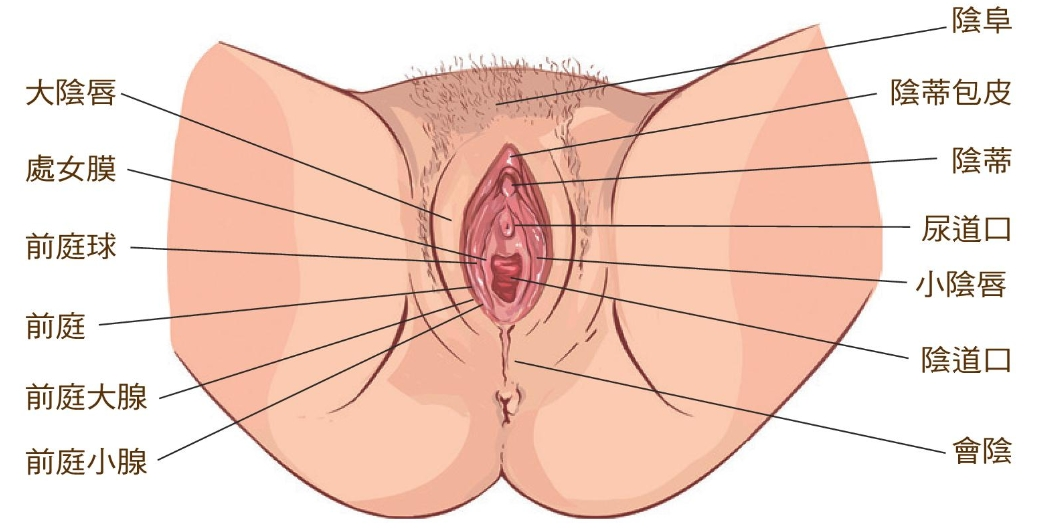
\includegraphics[width=0.7\linewidth]{7}
	\caption{}
	\label{fig:1}
\end{figure}

\begin{figure}[H]
	\centering
	
\includegraphics[width=0.7\linewidth]{8}
	\caption{}
	\label{fig:1}
\end{figure}

\section{内生殖器官}

\subsection{卵巢}

卵巢呈卵圆形,位于盆腔内子宫的两侧,左右各一。卵巢发育成熟后,能产生成熟的卵子,并分泌雌性激素,维持女性特征。在一个月经周期中,卵巢内常有几个甚至十几个卵泡同时发育,但一般只有一个发育成卵子。

\subsection{输卵管}

输卵管位于子宫两侧,是输送卵子进入子宫的弯曲管道。输卵管内端与子宫腔相通,外端游离。输卵管管壁由黏膜、肌层及外膜三层组成。黏膜上皮为单层柱状纤毛上皮。纤毛具有摆动功能。肌层的蠕动及纤毛的摆动,有助于受精卵进入子宫腔内。

\subsection{子宫}

子宫位于骨盆腔内,在膀胱与直肠之间,形状似倒置的梨子,前后略扁,分宫底、宫体、宫颈三部分,上通输卵管,下接阴道。

子宫是孕育胎儿的器官,又是产生月经的场所。子宫壁共分三层,由外向内为外膜、肌层和内膜。

很多女生在怀孕时会频尿,就是因为子宫变大,压迫到膀胱的缘故;也有女生在怀孕时痔疮发作,也是因为子宫变大,腹部压力变高,导致肛门和直肠附近静脉曲张所造成的。

\subsection{阴道}

阴道是一种收缩性很强的肌性管道,上通子宫颈管,下开口于阴道前庭,阴道前壁紧贴膀胱和尿道,后壁与直肠相邻。阴道为性交器官,又是月经排出和胎儿娩出的通道。

\begin{figure}[H]
	\centering
	
\includegraphics[width=0.7\linewidth]{3}
	\caption{}
\end{figure}

\textbf{阴道分泌物}

巴氏腺(大前庭腺)位在阴道口附近,会在性刺激时分泌一些黏液状的物质,而子宫颈和阴道内也有一些腺体会产生分泌物,让阴道保持正常湿润。

阴道分泌物在不同的生理周期会产生变化,例如在排卵期,分泌物通常会变得比较黏稠,有时会像生蛋白样。如果在小阴唇的皱褶上看到一些白白的碎屑状物质,这也是阴道的分泌物,如果不觉得痒,属正常现象。另外,在怀孕期间、生产后、停经前后等,分泌物的状态也会有所不同。

很多私密处用品厂商会告诉你,分泌物产生变化就是有问题,要你赶快去买这些东西来排除困扰,这完全是销售话术。其实在正常范围内的分泌物变化是不用担心的,但必须懂得分辨分泌物是否为正常状态,可依以下条件判断:

1.有一点味道是正常的,女性阴道的分泌物口交时尝起来稍微酸酸的,但不应该有强烈的味道。

2.经期之外,除了透明或淡白色,阴道分泌物不会呈现其他颜色。

如果只是感觉分泌物较多,有点不舒服,通常不会有什么问题,但如果是出现搔痒、痛感,或者是颜色和味道有明显的变化,那就应该去看医生,确认有没有感染,而不是私自购买那些宣称有疗效的私密处保养品来用,以免耽误治疗!

\textbf{阴道内的正常菌丛有助维持健康}

阴道内的环境不单纯只是由人体的分泌物构成,还有许多细菌也在里面扮演了重要的角色,这些细菌被称作“共生菌”,也就是正常状态下自然存在阴道内的多种细菌,如果没有它们的存在,阴道也没办法保持健康、正常的运作,多数情况下,这些细菌的存在对人体无害,甚至是有助平衡阴道的 pH 值,让阴道的菌落维持健康。

阴道内的正常菌丛还可防止入侵的细菌附着在阴道壁上,进而防止坏菌入侵。如果阴道内正常细菌的平衡状态被破坏了,就可能会导致感染和发炎。

常见的阴道共生菌,包含了厌氧性的革兰氏阴性杆菌和球菌,乳酸杆菌则会让阴道的 pH 值维持在正常浓度(正常阴道内酸碱度范围在3.8--4.5之间,为弱酸性),这能防止其他有机体在阴道内生长。

如果阴道的 pH 值增加,变得比较不酸,乳酸杆菌的质或量就会下降,让其他细菌有孳生的机会,进而导致感染,例如常见的细菌性阴道炎或念珠菌阴道炎,这些疾病可能造成搔痒、刺激或是导致分泌物异常。

\textbf{紧不紧,很要紧?}

很多对性知识好奇的人心里都抱着一个疑问,那就是女人阴道的松紧度与性爱满意度有没有关系?经过研究显示,女性的外阴构造与男女之间的性满意度没有多大关联,女人阴道的性功能主要是由心理因素决定,而非生理因素。

女性的阴道长度有7--12公分,宽度可容纳两根手指,阴道壁有许多橫行的皱壁,有较大的伸缩性和弹性,兴奋时阴道深度会增加1/3,宽度也会增加,所以一般不会出现男女性器官无法配合的情形。未生产过的女性,阴道通常不至于太宽松。

女性分娩时,直径达10公分的胎儿头部也能通过阴道,这就可以证实女性阴道有很大的弹性,所以这方面的担心是完全没必要的。

但初夜性交时女性下体会疼痛,大多是由于心理紧张、经验不足等其他因素导致,和器官本身通常没有直接关系。

有些女性则在生产过后会有阴道松弛的现象,造成性生活满意度降低,若有这种情形,可透过阴道紧缩手术来改善。阴道紧缩可使男性在性交时较有快感,女性也能藉此达到高潮,增进夫妻情感。

女性性高潮来源于阴道括约肌强烈收缩,继而刺激性感带,若是耻骨尾骨肌收缩不够强烈,或是在生产时受到创伤又没有修补,就不太容易在性交时享受到高潮了。

\textbf{“高潮”来袭,耻骨尾骨肌会出现规律性收缩}

女性性高潮来袭时,耻骨尾骨肌会以每0.8秒的频率收缩一次,产生反应后,子宫也会以每0.8秒的频率上下“抖”动(子宫高潮),这一系列的收缩抖动就是高潮来临。女性性高潮的享受感比男人强许多,男性性高潮的时间约只有8秒,女性可达20秒以上,女性之所以能在短时间内享受极致的性高潮,耻骨尾骨肌的功能很重要。

女性性爱时若没有高潮的感觉,可以做以下练习:把3支手指头放入阴道内,收缩阴道,使手指可以感受到收缩的力量,尤其是30岁以上的女性,1天做2次,1次15下,连续两周。但有一些年纪较大的女性,即使每天练习也无法自主控制肌肉的收缩,若想恢复功能,就需要借助“阴道整型术”了。

阴道紧缩整形手术一般分为三种:

1.后阴道壁整形术:强化直肠脱出与阴道松弛,这也是一般夫妻因为抱怨阴道松弛最常做的手术,做法是先把阴道壁黏膜分开,接着把提肛肌强化缝合,切除多余的阴道黏膜,再根据自然生产的会阴缝合术,重建强韧的阴道壁。

2.前阴道壁整形术:可同时改善膀胱脱垂的症状,手术把前阴道壁黏膜分开,接着把子宫膀胱筋膜韧带加缝一层,再强化膀胱底部及尿道的支撑力量,最后把多余的阴道黏膜切除再缝合就可以了。

3.生产时顺便做会阴整形术:修补会阴缺口处再重新缝合,此时可以同时把阴道内部松弛的表皮切除一部分,再拉回缝合,使阴道回复产前的紧实状状态。

阴道整形手术对妇产科医师来说是简单、快速的手术,过程只要20--30分钟,如果你有这方面的困扰,只要一个简单的手术,就能改变夫妻间的性生活与互动关系,千万不要讳疾忌医。

\textbf{蒙娜丽莎之吻私密雷射}

怀孕、生产,乃至更年期变化,是多数女人一生都不可避免的历程,但随着生产伤害、荷尔蒙变化及人体正常的组织老化,会使阴道出现松弛、干涩、易感染、漏尿等问题,不仅让自己性趣缺缺,也影响另一半的“性”福。

对于这样的困扰,医界过去多是建议患者做凯格尔运动,情况严重的只能直接以手术处理。近年来,美容医学界发展出私密处紧实雷射,不需动刀或住院,便可有效改善上述症状。它的原理类似运用在脸部的飞梭雷射,只是将施打的位置转换为阴道内/外阴部等地方。将雷射探头置入阴道后,运用雷射的光热效应,汰换老发黏膜,刺激胶原蛋白重组新生,黏膜增厚,可达到让阴道环境年轻化、健康化,并能提升湿润度、包覆感,及对尿道支撑度。改善漏尿等效果,对于性生活满意度也有很大的帮助。

\textbf{有问必答}

Q:哪些人适合做阴道紧缩术 ?

A:
1.生产过的女性(无论用哪一种方式生产)。

2.阴道曾经有过撕裂伤。

3.性伴侣阴茎尺寸较小。

4.想要借阴道紧缩提升性交满意度。

5.阴道松弛状况严重者。

6.40岁以上因为胶原蛋白流失,阴道壁变薄,阴道变松、变宽。

\section{护理}

私密处的清洁

女性对于脸部、身体、四肢的保养通常都很在行,但对于私密处的清洁与保养就没那么清楚了,以下是照顾私密处的要诀:

1.每日清洗:女性外阴部由于油脂、汗液及阴道分泌物较多,加上阴道口、尿道口和肛门紧邻着,尿液、阴道分泌物和粪便容易交叉污染,且外阴的皮肤皱褶比较多,这些特点有利于病菌滋生、寄居和生长繁殖,因此一定要做好外阴的清洁卫生工作,正常情况下每日清洗1--2次,在做爱前尤其必要再清洗一次,因为男人口交时会一再重复舔舐女人的阴部。

2.使用温水:不能用过热的水清洗,热水会造成局部的刺激和损伤,最好也不要使用冷水,冷水会让外阴部感到不适,也不容易将分泌物洗干净。外阴皮肤是女性最娇嫩的皮肤之一,非常敏感,人体会分泌油脂来保护它,经常使用清洁剂洗去这些油脂,容易引起外阴皮肤干燥,甚至发炎,加上清洁剂若为碱性,经常使用就有可能会破坏阴道的酸碱平衡,导致阴道炎等疾病发生。

3.清洗顺序:清洗外阴前应先洗净双手,然后从前向后清洗大、小阴唇,最后洗肛门周围及肛门;不能从后向前洗,以免将肛门部位的细菌带入阴道。

4.清洗方式:最好淋浴,如果无法淋浴可用盆浴代替,但要使用专用的浴盆。

5.挑对清洁用品:阴道内的 pH 值大概在3.8--4.5,外阴部的 pH 值则在5左右,有些清洁用品会标榜弱酸性,接近阴道的 pH 值,事实上,外阴部的洗剂不用这么酸,因为外阴部其实也没有这么酸。阴道及外阴部有自我调节 pH 值的能力,就算用偏碱一点的洗剂,身体很快就会调节到正常的 pH 值。所以,只要不是刻意用特别酸或特别碱的产品,且长期、频繁地使用,原则上是不必太过担心的。

照顾私密处的注意事项

每天好好清洁私密处其实已经够了,但如果希望给外阴部什么特别的保养,基本上只要挑选成分不要太花俏,不要有香精、色素、刺激性成分,或者含有容易产生粘膜刺激性防腐剂的产品就可以了。

一般的清洁用品多不会有什么问题,除非你是特别敏感的人,会因为使用一般产品而感到干燥、干痒或是其他不适,否则不需要使用特别的清洁产品。

另外,太过闷热的环境容易造成外阴搔痒,甚至是起疹子,因此穿着比较通风的裙装,避免穿材质对外阴部容易产生摩擦的内裤,也是做好外阴部保养的基本工作,挑选内裤时以纯棉材质为优选。

很多女生觉得经血脏,因此在月经期间会特别冲洗阴道,甚至买一些灌洗用具,例如阴道冲洗器,其实这是没有必要的。月经其实就是子宫内膜剥落后的产物,它和子宫颈分泌物及其他阴道内分泌物,都是人体正常代谢的物质。经血从阴道被排出的过程,其实就是人体在做自我清洁了。

还有一些女生会担心自己下体的味道不好,但正常人的阴道分泌物,本来就会有淡淡、酸酸的味道,如果想要追求无味或是香香的气味,通常只会弄巧成拙。具有香氛的产品对阴道保健完全没有帮助,反而可能破坏阴道的自然平衡。

想做好私密处保养,还需要注意以下几点建议:

1.与不甚熟悉的、或有多位性伴侣的男性性交应全程使用保险套:这能保护自己也保护别人。有些病毒和细菌在性交时会进入阴道,包括造成衣原体感染、淋病、生殖器泡疹、尖锐湿疣、梅毒和 HIV 的细菌和病毒,性交时戴保险套可防止这类感染发生。

2.定期体检:如果发生过性行为或是30岁以上的女性,建议定期做子宫颈抹片及性病系列检查。

3.规律的作息与运动:规律的作息可确保身体有正常的免疫能力,让阴道内菌丛维持好的平衡;规律的运动可强化骨盆底肌肉,对整体健康有帮助,而要锻炼骨盆肌,可尝试走路、跑步、游泳等运动。

4.选用正确的清洁用品:选用温和、不刺激、不添加香精的清洁用品,有些产品宣称草本、天然、无毒,不一定比较好。

5.不需过度清洁阴道:不必使用任何阴道内灌洗用品,也不必特别清洁阴道内的月经血块,如果因为感染有必要特别清洁,医师会开立药品,不要自行灌洗,避免因此破坏阴道内正常的菌丛生态。

6.如厕后不建议使用湿纸巾:这类产品可能含有较高浓度的防腐剂或香精,长期使用对身体不好,用卫生纸就可以了,还要保持外阴部通风、凉爽、不潮湿。

\chapter{男性生殖器官}

男性生殖器官分为外生殖器官和内生殖器官两部分。外生殖器包括阴阜、阴囊和阴茎,而内生殖器由睾丸、附睾、精索、输精管及射精管、精囊腺、前列腺、尿道球腺、尿道等组成。

\begin{figure}[H]
	\centering
	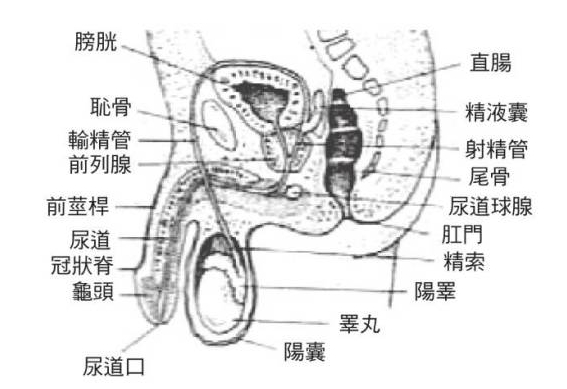
\includegraphics[width=0.7\linewidth]{4}
	\caption{}
\end{figure}

\begin{figure}[H]
	\centering
	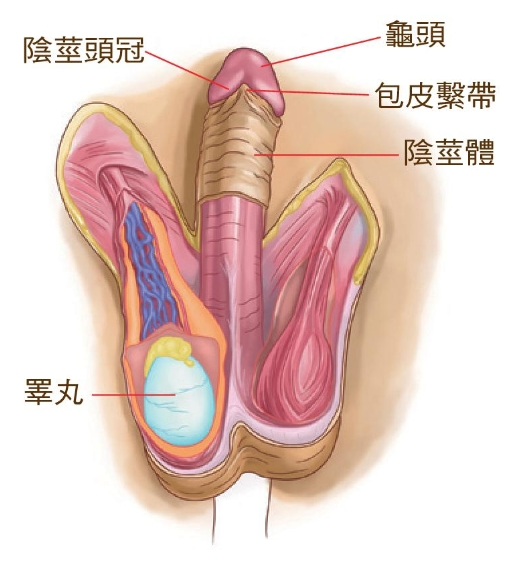
\includegraphics[width=0.7\linewidth]{13}
	\caption{}
\end{figure}

\section{外生殖器官}

阴阜为耻骨前方的皮肤和丰富的皮下脂肪组织。青壮年时阴阜显著隆起,中年以后脂肪组织减少下陷,老年则萎缩变平。

阴囊是由皮肤、肌肉等构成的柔软而富有弹性的袋状囊,里面有睾丸、附睾、精索,主要功能有保护睾丸、调节温度、有利于精子的产生和贮存等。阴囊内有阴囊隔,将阴囊内腔分成左右两部分,各容纳一个睾丸和附睾。阴囊皮肤薄而柔软,并有很多的褶皱。阴囊皮肤有明显的色素沉着,长有稀疏的阴毛。

阴茎后部为阴茎根,中部为呈圆柱形的阴茎体,其前端膨大部分为阴茎头(俗称“龟头”)。阴茎轴与阴茎头之间是冠状沟,阴茎头与冠状沟含有丰富的神经末梢,对刺激是很敏感的,而冠状沟处神经分布最丰富,敏感性最高。阴茎体由阴茎海绵体和尿道海绵体组成,具有丰富的血管、神经、淋巴管。从外形上看,阴茎有松弛和勃起两种状态,具有排尿、性交、射精三大功能。

\subsection{阴茎}

\subsubsection{阴茎多大才算正常}

阴茎大小存在着明显的年龄差异。儿童期男性的阴茎较小,到了青春期阴茎开始长大,且颜色加深,成年后相对稳定,但其长短不一、粗细不等属正常生理现象。阴茎大小有一定范围,但多大才算正常,这并没有一定的医学标准,一般通过测量阴茎长度(自阴茎根部到尿道外口)和阴茎周径来衡量。泌尿外科专家曾对一百例进行婚前体检的正常男性青年做了常态下阴茎测量,其测量结果发现,阴茎长度在6--9公分的人共93人。一家医院泌尿科测量结果证实,一般青年男性的阴茎平均长度为6.55公分(未勃起状态下)。一般认为,我国男性的阴茎长度多在6--9公分之间,阴茎周径多在7--9公分之间。但这并不是评定阴茎大小是否正常的标准,也不能说明不在此范围内的阴茎就一定不正常。一般情况下,阴茎的大小对性生活不会产生实质性的影响,除非过大或过小。

阴茎大小存在个体差异,能够影响阴茎大小的因素有很多种,包括身体脂肪过多、天气过冷、压力等,但与身高没有直接关系。性医学专家认为,阴茎大小主要与种族和遗传有关。一般认为同等身高,白种人与黑人的阴茎要大于黄种人。阴茎大小也受遗传因素的影响。

\section{内生殖器官}

睾丸是男性生殖腺,呈卵圆形,左右各一,由精索将其悬吊于阴囊内,长约4--5公分,厚约3--4公分,约重15克左右。睾丸是产生雄性生殖细胞(即精子)的器官,也是产生雄性激素的主要内分泌腺体。

附睾位于睾丸的后外侧,外形细长,似半月形,左右各一,长约5公分。附睾有储存和排放精子、促使精子成熟及供给精子营养的作用。

精索位于睾丸上端至腹股沟管腹环之间,左右各一,全长约14公分。精索是睾丸、附睾及输精管血液、淋巴液循环的通路,也是保证睾丸的生精功能及成熟精子输送的主要途径。输精管是精索内的主要结构之一,其末端与精囊腺的排泄管汇合成射精管,穿过前列腺,开口于尿道,全长约40--46公分,直径约2--3公厘。

输精管是精子从附睾被输送到前列腺部尿道的唯一通路。射精管是输精管壶腹与精囊管汇合之后的延续。射精管很短,长仅为2公分左右,管壁很薄。

精囊腺为一对扁平长囊状腺体,左右各一,表面凹凸不平呈结节状,其末端细小为精囊腺的排泄管,与输精管的末端汇合成射精管,在尿道前列腺部开口于尿道。精囊长4--5公分,宽约2公分,容积约4C.C。精囊为屈曲状的腺囊,其分泌液主要为精浆液,占精液的70\%左右,对精子的存活有重要作用。

前列腺为一个栗子状的腺体,平均重量约20克,是男性最大的附属腺体,能分泌前列腺液,组成精浆液。前列腺还被认为是一个性敏感部位,对其进行适当刺激时,可以引起性兴奋。

尿道球腺左右各一,位于尿道生殖隔上下筋膜之间的会阴深囊内,开口于球部尿道近端,可分泌少量液体,为精浆的成分之一。

男性尿道长12--20公分,既有排尿功能,又有排精的功能。其中有尿道球腺,可分泌液体,参与精液的组成,性交时有润滑阴茎头的作用。

\part{性欲}

简单地说,性欲就是对性生活的一种欲望,它既受体内激素水准的调节,也受社会、家庭等周围环境因素的影响。同时存在比较大的个体差异,即使是同一个人,性欲的高低也随年龄、心理状态、患病状况、生活品质、工作环境、婚姻状态等不同而表现不同。

一般情况下,性欲源于性心理的驱动,比如对异性的爱慕可以诱发性欲。男女之间建立美满家庭以及夫妻间的亲昵,都会产生性交的欲望。性欲产生的另外一个原因与内分泌有关。青春期过后,骤然提高的人体性激素分泌水准会驱动性欲。男性精囊、前列腺等性腺内分泌物的增加与淤积,女子外阴前庭大腺等分泌物的过多贮存,都可诱发性刺激和促进性欲。此外,既往性生活的愉快感受,或者男女之间身体接触产生的性刺激等,也可以诱发性欲。所以,性欲是多方面因素综合作用的结果,不但思维、意识、情感、环境等因素与性欲相关,而且语言、文字、图画、音乐等,也会给性欲带来举足轻重的影响。

\chapter{男人的性欲和女人的性欲一样吗?}

从表面上看,男人的性欲似乎比女人强,因为在性生活中居于主动地位的女性比较少,这里面既有生理上的因素,但主要还是心理因素的影响。许多女人习惯于压抑自己的性需求,所以,在多数情况下,男人的性欲表现得比女性主动,但这不证明男人的性欲就比女人的性欲强。

处于青春期的男性比女人更富于性幻想,并容易将感情需要和性需要混为一谈。成年以后,工作的压力和家庭的负担,会使青春期旺盛的性渴望减弱,但仍有少数人性欲一直比较强烈,在这一点上,女人和男人是一样的。男性的性欲在某些年龄阶段表现得要比女人强,但在另一些年龄阶段却可能完全相反。在性生活不和谐的夫妻中,产生性欲低下的一方往往是丈夫,其中年龄是个重要因素,男人的性欲高潮期通常在30岁以前,而女人则是在40岁左右,才对性活动表现出浓厚的兴趣。

\chapter{为什么有的人性欲强,有的人性欲弱}

性欲是有很大的个体差异的。性欲的强弱程度与下列因素有关:

1.遗传因素:性欲的强弱程度受遗传因素的影响,一个家族的成员,往往表现出类似的性欲倾向。

2.激素水准:人体中有多种激素,男女皆然。在多种激素中,雄性激素对性欲的影响最大。雄性激素水准高,性欲就强,雄性激素水准低,性欲就弱,无论男女都一样。

3.感觉刺激:在多种刺激下,人体就会产生各种各样的感觉,如视觉、味觉、听觉、嗅觉、触觉等,这些感觉可以激起性欲,在这一点上男性和女性没有明显差异。

4.性体验和性经验:如果以往性体验顺利并且性经验丰富,性唤起就比较容易;反之,性欲的产生就比较困难。

5.环境因素:人体会对外界环境的刺激作出多种反应,所以生活环境中的光照、温度、湿度、季节、饮食等因素,都会影响性欲的产生。

6.文化因素:性欲的产生是一种个人行为,但性欲也与文化因素有关,在某种程度上它必须接受伦理、法律、道德,甚至医学的约束。

7.情绪变化:心理状态影响着性欲的产生,比如当人们被忧虑、恐惧、愤怒、抑郁、疼痛、痛苦所困扰的时候,一般是很难产生性欲的。

8.年龄因素:人的性欲会随着年龄的变化而变化。就一般规律而言,男性的性欲高峰在30岁之前,而女性则是在40岁以后性欲最为高涨。随着年龄的增加、内分泌的改变,体内雄性激素的减少,人体感觉会变得迟钝,导致性器官血液循环不良,再加上来自事业、生活及社会交往等方面的压力,这些因素都会使人的性欲减退。

9.健康因素:健康的生理状态是维持性欲的基础。人体的各种疾病,如内分泌、生殖器官、代谢系统、肿瘤及其他消耗性疾病,都会影响性欲的产生。

总之,性欲是人的生理本能之一,它受多种因素的影响。

\chapter{不要将性欲望和性功能混为一谈}

现实生活中,不少人对性都存在认识上的误区,将性欲望和性功能混为一谈即是其中之一。实际上,这两者还是有区别的。

所谓性欲望是对性的一种要求、一种渴望的心情,而性功能则是将欲望化做具体行为的能力,完美和谐的性生活,需要性欲望和性功能的协调和统一。如果能将性欲望和性功能协调于一身,就能充分享受性所带给自己的愉悦;但是要想实现这个愿望,需要不断地摸索和探寻,如果没有完成这种转化,就会导致性的各种不和谐和性功能障碍。

实际上,性欲望和性功能分离的情况是很常见的,常见原因有生理性的,也有精神心理性的,还有疾病等因素。比如,进入青春期的青少年,开始出现朦胧的性意识,也具有了阴茎勃起的能力,但他们对性的欲望还没有建立起一个明确的概念;一个习惯自慰的青年,有可能担心自己患了阳痿,怀疑自己的性能力;老年男性,尽管岁月的磨练使他们更加珍爱生活、珍爱爱情,对于性的要求(欲望)也很高,但是性功能却在慢慢地减退,直至消失;患有某些疾病的男子,尽管主观上很想“要”,但实际能力却不行;某些传染病患者,尽管性功能很好,但为了疾病的康复,必须抑制自己的性欲望。

\part{性生活}

\chapter{性生活不仅仅意味着性交}

性生活是夫妻间表达感情、传递爱意的重要手段。在正常的夫妻性生活中,即使男性最终出现了高潮和射精,但这也并不是性生活的全部内容,更不是它的首要目的,性生活还包括夫妻双方的精神交流、性生活中的默契配合和性交后的恩爱,性生活的品质,在很大程度上,取决于全部过程的圆满程度。

有些人常把性交过程看做是第一位的,于是导致了性生活的过于急切、粗暴和简单的程式化。丈夫容易忽视妻子的情感需求,把性生活简化成一系列的动作,甚至有人为了显示自己“性能力强”,而粗暴地强迫妻子与自己过性生活,极大地伤害了妻子的人格与情感。这种“性”多、爱少的方式,只会给对方带来痛苦和厌恶,而不是身心愉悦。其实多数女性最看重的并不是性交的过程,而是相互温存的感觉与感情交流。

有关调查显示,夫妻中大约有四分之一的人几乎从不相互亲吻;差不多有一半的男性很少抚摸妻子,但他们均认为自己的婚姻生活是和谐美满的,或者是比较满意的。由此可见,多数男人往往是过分地偏爱最终的性交过程,这种现象在乡下更为普遍,有些人只是把性看作是一种生活内容,是必须履行的义务,而不是为了传递爱。

现实生活中,家庭、职场有很多问题都要面对,身心疲惫的情况会时有发生。如果夫妻中的一方想要过性生活,而另一方则状态不好只是勉强为之,那么性生活结束之后,不仅主动的一方会觉得毫无兴致,而被动的一方也会更加难过甚至痛苦,长期下去会形成恶性循环。事实上,越是突发地匆匆行事,就越是极其狭隘地理解性生活的内容,也就越缺乏交流和深切感受,身心疲劳也就越是加重,结果把性生活变成消极、冷漠和缺乏激情的“机械化运动”,夫妻双方难以体会性生活带来的愉悦感,甚至出现性功能障碍和性冷淡,并由此丧失了爱心、情趣及性的和谐之美。过去这种情况在中年男人身上比较多见,但近些年一些年轻人,甚至新婚不久的男性也抱怨“没意思”,其实是同样的原因所导致。因此,无论男人还是女人都应该切记:为了爱而性交,而不是为了性交而性交。把握好这个基本点,一切的问题也就顺理成章地容易解决了。

\chapter{性生活的几个阶段}

性生活大体有四部分的内容,即性交的预备、性器的交合、性行为的运动、性交的结束。这个过程又可以分为兴奋期、平台期、高潮期和消退期。

\begin{figure}[htbp]
	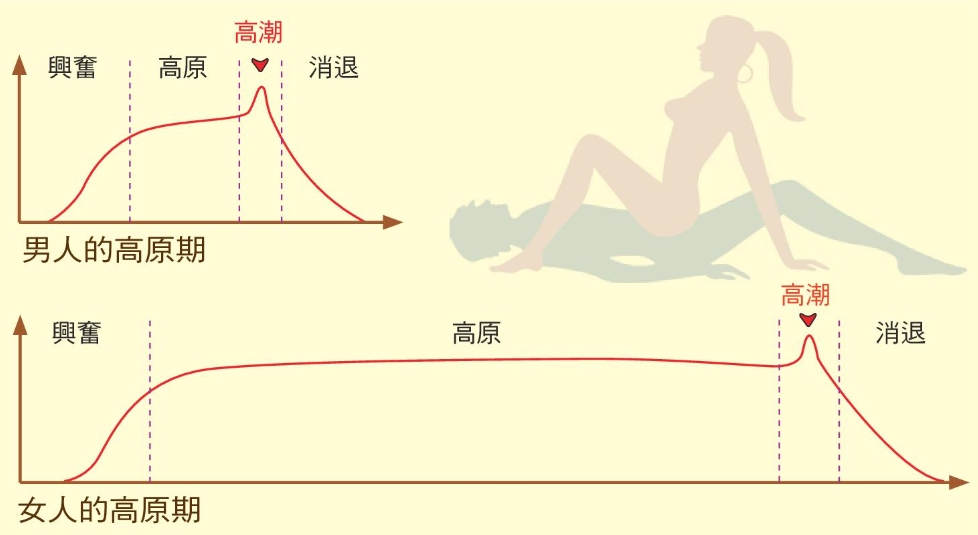
\includegraphics[width=1\linewidth]{6}
	\caption{}
	\label{fig:1}
\end{figure}

1.兴奋期:在肉体或精神上的性刺激下,性欲被唤起,身体开始处于紧张阶段。

性交是夫妻生活的重要内容,关关到夫妻感情的和谐与否,所以夫妻双方不应草率从事或敷衍应付,在性交前要做好充分的准备工作。在性刺激下,男女双方的性器官都会逐步处于充血状态,男性阴茎膨大了,女性阴道也有变化,但这些变化所需的时间,男女有很大的差异。当男性的性欲达到一定的程度,阴茎勃起变硬时,多数男人着急要进入下一步工作,但女方性欲的激发,往往需要一定的时间,短的需要几分钟,长的可在半小时以上。当然,有性交经验以后,夫妻之间的差异会缩短,并基本保持一致。

性交时男女双方的体内,都会分泌出具有润滑作用的液体,有助于激发性兴奋。此时男性阴茎上端的阴茎头被润滑的液体所滋润,女性阴道外及阴道内壁也都分泌着这种物质,男性阴茎靠着这些润滑的液体,插入女性阴道会变得容易,但是如果男性性急,在这种润滑的液体分泌之前,便要插入女性的阴道,再加上动作粗暴,不但容易使女性受伤,也会使女性产生恐惧性交的心理,还会给自己的性器官带来明显不适(疼痛甚至损伤),给以后的性生活造成障碍。所以在性交前做充分的准备工作是非常重要的。

2.平台期:即性高潮前期,在这个阶段的基础上,身体的性紧张逐渐到达顶峰。

3.高潮期:持续时间很短,大约只有几秒钟的时间,高度紧张的肌肉经过痉挛,处于放松的状态,使人获得快感。

首先是宣泄后的轻松感。男性在性刺激下产生性兴奋,阴茎勃起,产生交媾的欲望,达到射精。射精之后恢复平静,心境弛缓,获得宣泄后的满足,这是性快感的内容之一。

女人的高潮和男人不同,首先她的优势是不必有压力,性交时阴道以逸待劳,阴蒂也不如阴茎勃起有时间的压力,女人可以放松享受一段相当长的高原期,男人的高原期可就没有那么长,且在过程中精神是十分紧繃的。

一般来说,如果直接刺激女性阴蒂,平均要花20分钟能让女人达到高潮,而男人大概只需要刺激阴茎2--5分钟即可达到高潮。

4.消退期:身体由紧张逐步松弛和消散的过程。

性生活的不同阶段,男女双方的身体都会出现相应的生理变化,但是这种变化是存在很大的个体差异的。

男女在做爱过程的享受主要是高潮前这段高原期,所有的姿势变换、技巧施展、情趣製造、高潮蘊釀,都宜在高潮前这段时间。

男人做爱时若想持久一些,就会拼命想扼止高潮射精的冲动,相反地,女人这方是一心一意想要向高潮推进,到高潮之前不希望停下来,如果男人太早射精,无异宣告做爱结束,会令她大失所望。

若要分析男人做爱时的心理,勃起愈久愈能满足他的自信心,因为这表示他在床上有足够的能力让自己心爱的女人感到满足,如果总是草草结束,老是让女人失望,他会深深觉得对不起女伴。

也许女人一般不太了解男人,男人把性的成就和事业的成就同样列在人生至高的位階,即使古代的皇帝也不例外。皇帝在事业的地位居于人群顶峰,在性事上也享有绝对的优势,但仍然上窮碧落下黄泉要寻找壮阳药,这么做在于他不单要享受与更多女人做爱,更重要的是,他要让每个女人与他做爱时都得到满足。看吧,连贵为皇帝都需要拥有性的成就感!

但在性爱享受这件事,上帝真的是比较厚爱女人,女人全身无一处不能成为男人眼中的性感誘惑,主要原因在于男人对性的感觉是经由视觉而起,有一句成语说“秀色可餐”,或可把它理解成“女人身体的任何一个部位,都可能在男人的惊鴻一瞥之下成为性感带”!

日本知名作家川端康成在小说《伊豆的舞孃》中,有一段描写女人在雨中的街道行走,露出一双被雨淋湿的小腿,显得格外白皙细嫩,所以男人很自然的在做爱开始时就迫不急待又舔又吻女人的身体。

另外在日本着名漫画家弘兼信史的暢销作品《課长島耕作》系列漫画中,有一段描述某知名跨国大企业老社长特别喜爱吃女人的小腿,他每次下班后便去銀座的居酒屋,她寵爱的女人会把双足洗得干干净净,让老社长把她的腿当珍饈吃,甚至可以把五个脚趾及半个脚掌全含进嘴里。乍听之下頗让人难以置信吧!不过請各位女士们用心了解,这些都是男人真誠表现性欲的不同面相。

性爱是人类生活的重要组成,它在很大程度上影响着人们的身心健康。

国外一项对37500个成年人性生活的调查显示:性生活主动活潑的人较少焦虑,不常出现暴力和敌意,也更少抱怨,更少把不幸、不快乐的责任推到别人身上,因而也就更少和人们处在冲突和紧张的关系中。研究还发现,性生活对人体免疫系统有支援作用,有助减缓疼痛,调节内分泌,改善精神状态,且很多益处只有在长期拥有良好的性生活后才得以逐渐体现。

以下列举几项性爱的好处:

1.可以减轻压力:如果你工作了一整天,或觉得有点喘不过气,性行为可
以帮助你放松并减轻压力。在性爱过程中,我们的身体会释放出多巴胺、内
啡肽跟催产素,帮助我们对抗压力,提升快乐与热情。

2.燃烧热量,有助瘦身:说到“运动”,很多人都会提不起精神,但做
爱其实就是一项很好的运动。透过性交,我们的身体不断经历跟运动一样的
过程,例如提升呼吸率、燃烧卡路里(2500卡路里/次),一周若有三次性行
为,可燃烧7500卡路里,这相当于跑了75公里!

3.可提升免疫力:美国宾州威尔克斯大学的
学者发现,一周有两次性行为的人比起完全无性生活的人,身体里含有较多的特定抗
体。在性行为的过程中,可对抗一般感
冒与流感的免疫蛋白球A会被释放,更
好的是,性行为越频繁,免疫蛋白球会
释出越多,你就会变得越健康。

4.可降血压:英国佩斯利大学研究发
现,性行为可降低舒张压,让人更健康。

5.让心脏更健康:当人体燃烧脂肪时,我们的心脏会变得更健康。新英格
蘭研究机构发现,有规律性生活的男性,得到心血管疾病的机率比没有规律
性生活的男性减少了45%。

6.能止痛:如果你的身体有一些不明的疼痛或偏头痛,性行为可能比止痛
药更有镇痛效果。关节炎专家尔利奇(GeorgeErlich)医生研究发现,没有
性生活的病患比有性生活的病患更常感觉疼痛。

7.帮助月经周期更规律:如果你的月经周期不太穩定,有可能是你的生活
充满压力,而性行为能帮助降低压力,所以对你的月经保持规律有益。

8.训练骨盆肌:不止四角肌、背肌与核心肌群,性行为还能训练你的骨盆
肌。英国国民保健署(NHS)指出,有了更强健的骨盆肌,你能更容易达到
性高潮。NHS还表示:对女性来说,强健的骨盆肌可减缓尿失禁的症状,同
时可增加敏感度,带来更强烈的性高潮。骨盆运动也有助男性解决性功能障
碍与尿失禁的问题。

9.降低罹癌风险:规律的性生活可降低罹癌风险,尤其是男性。在一项由
美国医学协会執行的研究中,一个月至少做爱21次的男性,罹患前列腺癌的
风险降低很多。

10.增进睡眠品质:就像运动一样,性行为能增强你的心肺功能,让你更
容易放松;另外,做爱还有舒眠效果,对此,加州西好萊塢心理医师安巴德
( Sheenie Ambardar)说,“性高潮后人体会释放催乳素,它能让你感到放
松,并有睡意。”

11.让你更显年轻:一周有3次性行为可以让你看起来比实际年龄少10
岁!性爱貧乏的女人因为缺少雌激素作用,脸色和肤质会相对显得暗沉,气
色也没有那么红润。

12.让你更长壽:美国加州大学旧金山分校(UCSF)的研究显示,女性
定期享受性爱可保护体内DNA,进而延年益壽。研究人員针对129名年龄介
于20~50岁的女性进行调查,訪问她们的性生活概况,并对她们进行血液測试,结果发现,有规律性生活的女性体内“端粒”(Telomere)较长,亦即
老化较慢,预期壽命也比较长。

“端粒”是染色体末端的DNA重复序列,和细胞老化有关。
通常,细胞愈老“端粒”愈短,细胞愈年轻“端粒”愈长。

性交可提高免疫机能
性交是一种很好的松弛剂,能使人安定下来,帮助入睡,是一种很好
的安定剂和失眠治疗剂。
美国紐约大学医学中心莫斯柯维茲(Reed Moskowitz) 博士认为:
“性行为是对现代文明生活中各种挫折的矯正剂。”当人处在紧张情境
之中,腎上腺素会大量分泌,然后进入全身,使肌肉紧张、血压升高、心跳加速,而这些紧张反应会損害身体的免疫系统,导致各种失常的情况出
现,例如感冒、高血压、胃溃瘍等。在性交开始的上升階段雖然有腎上腺
素分泌升高和肌肉收缩的情形,但高潮一来到就会使全身松弛下来。
尽管性高潮的松弛作用只能维持几个小时,但若是你有规律的性生
活,就会较少处于紧张状态,免疫系统的功能就能得到全面发挥。
另外,一项针对乳腺癌的研究显示,当性生活得到满足时,女性便能
进入一种生物化学上的快乐状态,此种状态可使人体释放出内腓肽,而内
腓肽具有很明显加强免疫功能的作用,还能提高T细胞浓度,T细胞正是免
疫功能的承担者;而且,仅仅是单纯的抚摸也能有助健康,爱抚可以提高
人体内5-羥色胺的浓度,而5-羥色胺可触发身体对抗疾病的细胞释放。

用进发退,
愈做愈爱
女性若长期缺乏正常的性生活或者性压抑,会导致性功能的发用性萎
缩,阴道分泌物减少或停止分泌,使得抗病能力下降,从而可能引起阴道感
染性疾病、子宫颈炎和盆腔炎等。近年来,乳腺疾病的高发人群也开始向年
龄较大、未婚、未生育的女性转移,而这与这类女性长期处于性压抑的状态
不无关系。
长时间没有性生活的女性容易对性产生淡漠的情緒,使得性功能下降,
甚至会提前进入更年期。人的生理功能都遵循着自然规律,当身体觉得这种
机能是不需要的,那么它就会结束使命。
性是女性身体里最晚成熟的生理系统,同时也是最早衰退的系统,人或
者动物,总是在性欲最旺盛、繁殖力最强的时候能力最强、最有创造力,这
是自然赋予生物的一种繁衍特性,当人的性能力衰退,人也就衰老了,各脏
器功能都会进入衰退期。

一般来说,女性长期缺乏性生活对身体的危害包括:
1.做妇科检查时会比其他同龄女性更加困难,同时疼痛感也会更明显。
2.会使性情较为压抑,而当人的心緒较为抑郁,就会导致睡眠品质不好,
睡眠品质差就会使人容易老化。
3.阴道分泌物减少或停止分泌,使得抗病能力下降,从而可能引起妇科相
关疾病。
4.容易对性产生淡漠的情緒,使得性功能下降,甚至提前进入更年期。
5.女性在节欲几个月之后性欲就会完全消失,要重新恢复性生活,喚醒性
欲的过程会愈来愈长。即使重新恢复性生活,也会出现因阴道分泌物减少而
有疼痛的感觉,同时还可能会有性高潮障碍的问题。

你可能不知道
根据《The Journal of Sex Research》杂识2018年5月公布“不同年龄层
性爱次数统计报告”显示:
30岁以下的人性生活频率是每周2.15次,每年约112次;
30~39岁的人性生活频率降到每周约1.6次,一年约86次;
40~49岁之间的人每年只有69次性生活。

迷思一:经常自慰容易导致性功能障碍
其实是这样:
自慰行为本身是无害的,真正会影响人们健康的,是因为自慰所产生的
自责、罪恶感、焦虑和恐惧的心理!
自慰是正常又能缓解性欲的方式,与性功能障碍没有因果关系。但因为
每个人的情欲高低不同,无法量化去制定所谓的“标准性爱次数”,所以,
只要不影响生活、工作、身体或精神状态,想自慰几次就自在享受。
迷思二:每次做爱时间至少要30分钟,才能使女人达到高潮
其实是这样:
有些男性为了要证明自己拥有极佳的性能力,拼了命去“做”,却忘了
对方的感受,殊不知,没有感觉的性,怎么能说是享受呢?做爱时间如果拖
得太长,反而像是在运动,不仅耗费体力,累死自己也弄痛伴侣,一点品质
也没有。要享受愉悦的性爱,建议多花点时间满足伴侣其他感官的享受,也
许在探索身体的过程中,就能开发新的愉悦体验。

有问必答
Q:做爱时间越长越好吗?
A:不一定!研究指出,一般男性大多
在5~9分钟就会达到高潮射精,而女性的性
满足也并非与性交时间长短成正比,性交时
间太长反而容易引起女性泌尿道感染,若男
性遇到迟泄或难以射精等困扰,建议立即就
医,寻找正确的治疗方式。

迷思三:女人都喜欢做爱过程中快、猛、用力撞击的感觉
其实是这样:
每个人都有自己喜欢的性爱嗜好与模式,刚开始交往的两人,需要从多
次的性爱交流来了解与熟悉彼此,因为你可能不清楚对方喜欢什么,所以学
習当个贴心的伴侣,试着引导对方说出什么方式、哪些技巧、力道如何最能
让她感觉舒服,只有充分沟通,才能让双方同享高潮。
迷思四:女人都喜欢“大老二”,太小、太细会被嫌
其实是这样:
从医学角度来看,阴茎完全勃起的长度如果小于7公分,就要检查是否有
包茎或萎缩等问题,如果没有,就不需要过度烦惱,因为女人阴道前段1/3靠
近阴道口处神经丛比较多,容易有快感,后段神经较少,因此阴茎长短或粗细跟高潮没有直接相关,最重要的是找对女人喜欢的方式与敏感带,才能享
受完美性爱。
有些男性受A片误导,认为影片里男演員的阴茎尺寸是“正常值”,相
比之下让自己很泄气,进而影响了性爱表现。事实上,影片中的男演員为了
让阴茎外观“好看”,付出了不少钱吃药或做整形手术,这样做雖然让阴茎
“中看”,但其实不一定“中用”。其实,男人阴茎在做爱时坚挺持久最重
要,这样才能提供女人最大的享受。
迷思五:每天都要“打手枪”就是性爱成癮
其实是这样:
性爱成癮的医学名称为“强迫性性行为”,指的是患者会无法抑制性
欲,而使生活失去控制的状态。如果你没有因为每天都要“打手枪”(男性
自慰),而造成身心灵失衡是不需要担心的,适当的“宣泄”(射精)其实
有利身体健康,研究显示,男性每个月射精次数超过21次,罹患前列腺癌的
机率少33%。

迷思六:女性胸部愈大,性爱完美度愈高
其实是这样:
一直以来,男人喜欢私底下討论女人胸部的大小,亦有资料显示,性爱
中男人最想亲吻女人身体的哪个部位?2%选择大腿,3%选择背部,4%选择
腰部,5%选择头发,7%选择腹部,8%选择双脚,9%选择臀部,10%选择私
处,12%选择手部,40%选择胸部。但是,已逝的文学大师李敖的意见是,
男人愈成熟,欣赏女人身体的注意力愈往下面部位移动,比如李敖挑女人首
先看她的小腿,他说年纪小的男人专看脸部,大一点、年轻的看女人的胸
部,成熟的男人喜欢看小腿。

正因为如此,让不少人以为,女性
的胸部越大,对性刺激的反应越强烈。
事实上这种观点是完全错误的,没有证
据证明女性胸部大小跟性反应的程度有
关。实际上,女性在胸部被人抚摸的时
候,胸部大或小的反应并没有差别。由
此可见,胸部大小其实是无须太过在意
的,罩杯大小,其实只是满足男人的视
觉感官,但在男人心中未必胸部大就性
感,适中而坚挺反而比较重要。
有问必答
Q:女人的阴道会不会因纵欲而松弛?
A:不会。女人阴道弹性限度远远大于男性阴茎的直径,不会因为做
爱的次数多而松弛,反而做爱次数愈多阴道会愈敏感。

Q:网路上说早上做爱比较好,是吗?
A:不一定!做爱的时间应该
挑在做之前不会过度劳累,且做之
后能充分休息的时间,不一定要在
什么时段,而是应该配合双方的时
间、精神和体力,但是男人在清晨
最容易勃起,所以利用清晨做爱是
最佳时刻。

做爱在于享受过程,
不必强求高潮
男人做爱真正的享受在过程,真正爽的地方在阴茎,阴茎抽送的时
间越久,男人享受的时间越长,做爱的姿势变化多一些,带给女人的快
乐更丰足。
男人一旦高潮射精,就好像戳破胀得满满的气球,顿时消气萎缩,
情緒随之跌落谷底!所以做爱时女人其实可以只管自己的享受,不必体
贴地担心他不射精,因为大多数男人要持久不易。当然,若是基于以下
两点理由,那就另当别论:
1.期待男人把精液射在自己体内。
2.有征服这个男人的满足感。

增强女人性欲的超級荷尔蒙DHEA
DHEA (Dehydroepiandrosterone,去氫皮质酮)的作用包括强化肌
肉、穩定产生性荷尔蒙、维持礦物质平衡、擴张血管、预防老化等,和雌
激素、雄激素一样,有回复青春的功能,因此有“抗老仙丹”、“荷尔蒙
之母”、“超級荷尔蒙”、“青春激素”等别名,它不但能提升更年期停
经女性心理及生理对性的渴望,同时也能提高阴道壁伸缩脈冲及阴道的血
流量,改善女人性冷感、增强女人性欲,且可长期服用。此外,它对人体
也有其他好处,例如,防止骨骼老化和动脈硬化、促进输卵管发育,对腰
痛、膝痛也有一定的改善效果。

别只是羞怯的
当个被动者

女人,当你想对男人表达温柔与爱意时,可透过亲吻对方的性器官与爱

抚,这么做,胜过千千万万句“我爱你”喔!记住,在性爱这件事情上,别
只是羞怯的当个被动者。
性器官一般都被称做耻部,因此不论男女,当自己的性器官被别人的嘴
唇或舌头触碰时,都会感到羞怯。而正因为这个因素,所以不管是亲吻别人
或是被人亲吻私密部位,都能让心理及肉体获得异常兴奋的性爱满足感。
但有很多女生抱怨:“雖然我亲吻了他的阴茎,但他却一点也不兴
奋!”其实,光只是亲吻阴茎是无法让他满足的。要知道,经由阴茎所带来
的高潮,技法不同,感受就会有天壤之别。为了加深彼此的性爱感受,互相
爱抚彼此的性器官时,应该先了解每个人不同的性感部位,这是很重要的,
然后再针对那些部位加以爱抚,这样一定能让两人的性爱越来越激情。
阴茎是让男人达到性高潮的部位,亲吻时要从最敏感的阴茎内侧包
皮系带开始,龟头冠、龟头沟等处的
感应最为强烈。女人亲吻勃起的阴茎
时,大部分都只是亲吻阴茎的前端而
已,其实这个前端部位,即使加以捏
按、吸吮,也不会有感觉,所以如果
女生要向男生表示对这个部位特别的
爱意时,光是吸吮前端部位,只会给
对方带来疼痛的感觉而已!

你必须知道,男性的性兴奋来源是集中在以龟头为中心的单点上。另
外,男性性器官还包括了睾丸和阴囊,这里的构造细致,所以很害怕受到撞
击,但是若能轻柔地拨弄爱抚的話,也是极易感受快感的部位,这个部位与
肛门间还有会阴部,此间密佈着精囊腺、前列腺等男性生殖神经系统,所以
只需用手指轻按、搓揉,就会很有感觉。
为什么男人都希望阴茎勃起更长久 ?
“早泄”指提早射精,换句話说,是勃起的时间太短暂,一般的医学论
述把早泄定义为“在阴茎插入阴道2分钟内即射精”。其实,2分钟对男人的
要求太宽容了!硬挺2分钟即射精,然后萎缩疲软,草草结束,女人的心理都

还没准备好,来不及享受就结束,好比看戏,才开始奏乐,主角还没出場,
幕就落下收場了,我想没有女人会满足的!

如果想让伴侣充份享受性爱,甚至进一步达到高潮,我认为需要20分
钟,但也许有人认为久一点更好,所以我想在多数女人心中,更适切的定义
应该是:在女人心满“欲”足达到高潮前,男人忍不住射精銘谢收场,都算
是早泄!
女人的呼喊:男人坚挺到我满意为止!
男人的希望:在我能够坚挺到女人满足之前,要忍住不射精!
其实在心理上,男人与女人对性爱的期待是殊途同归,互相契合的!
很多女人喜欢看男人高潮射精在自己的阴道中,这样可以感受到阴茎倏
忽间的膨胀,温热的精液喷在阴道里,那样的心理感受能带来无限的兴奋和
满足,两人常常能因此同步达到高潮!
但要怎么能达成这般完美的境界呢?前提是男人的阴茎必须能硬挺,且
维持足够久的时间,还要能抑制延迟产生高潮的冲动,但这个过程在男人心
里存在着双重矛盾。
女人啊,既希望自己的男人做爱时能达到高潮,可是又不愿意他太快射精,于是男人就必须压抑快感,但一直令女人困惑不解的是,男人在做爱过
程中的快乐到底来自哪里?
原来男人在勃起时心理上就会产生快感,这种快感会很快地进入高原
期,阴茎坚挺的时间越长,则男人和女人享受性爱的时间越久,一直到瞬间
冲到快感的最高点,这时的感受好比煙火射向天空的最高处,精液则好似火
花迸出喷向阴道。
射精之后,男人的性欲也瞬间消退,全身瘫软,体力耗尽,心情也在突
然放空后降至最低点,情緒进入低潮期,好比自雲端跌落谷底,而这个现象
和女人高潮之后的情况是迥异的。
一般女人认为,男人做爱时喜欢尽快达到高潮,其实恰恰相反,男人
做爱时会想办法不要太快达到高潮,总希望硬挺持久的时间能多一些,男人
的享受则是停留在高原期,想尽办法不要太快射精,因为只有硬挺的时间够
久,性爱过程才有足够的时间做变化。男人都知道,女人需要经过一段时间

的刺激后才能逐渐累积达到高潮的能量,多数的男人皆是如此,希望能尽量
满足伴侣,关于这一点用心,我想女人应该要多多肯定男人,是不是呢!
还要告诉你一个男人的小秘密,那就是:较多变换性交姿势,能让男人
保持较长时间不射精!
男人最害怕的事是在女人情欲正酣之际忍耐不住射精了,显得英雄气
短,所以在性交时,男人突然停住,抽出,要求改变体位,你应该要体谅
他,给他喘息一下,冷静一下,甚至体贴的问他要不要喝一口水,歇一下再
战,如果他很快就要求换体位,那你应该接纳他的意见,配合他,因为你的
性感使然,他可能一开始就太激动了,需要缓一缓!
有问必答
Q:女性在高潮时有极快乐和极度宣泄的感觉是怎么形成的?
A:由于前戏的性接触刺激,使神经冲动逐渐累积高漲,到最高点时如
河水决堤宣泄而出,这时女性的阴蒂会略微向上回缩,由于阴蒂此时极度
敏感,回缩可以闪避进一步的直接刺激,同时阴道底部鼓胀,呼吸急促,
脸頰及上身泛红,这在瘦削的人身上尤其易见。
女性在达到性高潮时,阴道肌肉会节奏性地每0.8秒收缩一次,但这种
反应的程度因人而异。在达到性高潮状态时,有些女性觉得每一条肌肉都
繃紧了,骨盆腔内充满了热血,全身舒暢无比,但也有些女性反应并不是
如此,她们只有一些温暖的感觉伴随着局部的肌肉收缩。
阴道这种每0.8秒节奏性的收缩也会受其他因素影响,如对性行为观念
的开放程度、专心程度、对环境安全度的感受、性行为频度、年龄及健康
状况等都有相关。
女性的高潮消逝得比较慢,如果再加以刺激,可连续出现高潮,不像男
性,必须要等数分钟、数小时,甚至数天(因人而异),才可以再射精。

掌握性事主导权

女人想要掌握性事主动权,可藉由挑逗男人开始,这很容易做,任何时间都可以,例如:

1.洗澡时:在男人洗澡时,你可以卸下全身衣物,悄悄潜进浴室,用香皂
抹他的肩、背、臀,及会阴、肛门,让男人先享受被服务的快感。然后从背
后将双手环绕至他身前,用香皂抹他的胸部、两乳,双手再顺势往下滑到男
人的阴茎,藉着泡沫的滑润,运用双手温柔灵巧的揉搓他的阴茎及阴囊,但
是不能按压,睾丸会痛,这些举动的目的是在挑逗他,也同时在享受玩弄男

人身体的乐趣,记得要轻声温柔地问他:“舒服吗?”

千万不要突然停下动作,因为你的目的不是替男人洗澡,而是在享受玩
弄男人身体的乐趣,要让他有足够的时间意识到你的用意,一旦他意识到你
的动机,男人必然会春心蕩漾!

\begin{figure}[htbp]
	\centering
	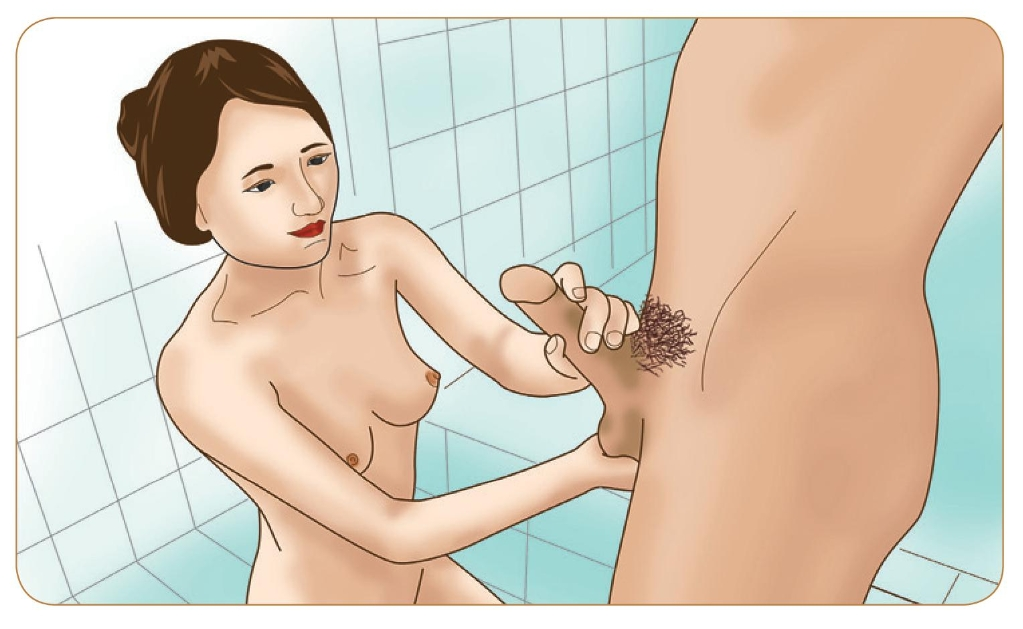
\includegraphics[width=0.7\linewidth]{14}
	\caption{}
	\label{fig:1}
\end{figure}

这时,你可以转到他面前,把自
己的乳房抹上滑润的沐浴乳,紧抱
住他,用双乳摩擦男人的胸部,并
且让一支手顺势滑下,男人的阴茎此
刻可能已经勃起,你可以用手指拾起阴
茎,用他的龟头碰触揉搓你的阴蒂、前庭
阴唇,千万要记住,你此刻的心态是在享用男
人,得到性快感,不必单纯只是在討好男人,所以维持多久由你决定!
接下来你可以面对他,蹲下,用手指拎起阴茎,开始含、舔,好似享用
美食一样,反覆舔舐龟头及阴茎干,同时要舔他的阴囊,提醒你,用舌头舔
舐阴囊给男人的快感胜过用口含着龟头,当然,当你把龟头含在口中时,务
必同时用舌头灵巧的绕着舔。
上帝把女人的身体塑造成凹凸有致是有意义的,因为女人好似花朶,
必须藉由芬芳的气味及繽紛的色彩来招蜂引蝶,让男人自投罗网,因此,挑
逗、引誘是女人采取主动性行为的极佳方式!

\begin{figure}[htbp]
	\centering
	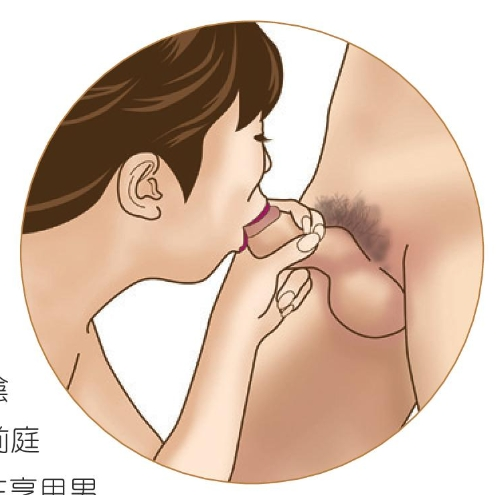
\includegraphics[width=0.7\linewidth]{15}
	\caption{}
	\label{fig:1}
\end{figure}

2.清晨:男人在清晨时分,阴茎常常会自动勃起,这叫“晨勃”,如果前
一天晚上女人想做爱,老公却推託说工作一整天身体很累,那么就让他好好睡上一觉,翌日清晨,你不妨悄悄的把手伸进他的裤襠,让手指有如对待小
寵物般轻抚他的阴茎,很快地,它就会悄悄勃起!
此时你不要只是见獵心喜,要记得先把自己的阴道口及前庭抹上足够的
润滑液,然后用手指托起阴茎,缓缓地坐上去,让阴茎插进你的阴道,在他

半梦半醒之间,两人一起享受一顿丰盛的早餐!但如果男人上午必须要开长
途車或从事重劳务则不宜,否则他很容易因为疲累而在工作时打瞌睡!
挑逗会让男人意识到你的情欲需求,但记得提醒他,满足你的性需求是
他责无旁貸的义务,他必须耗费一部份精神与体力和你共享性爱的欢愉。从

另一个角度看,也让他深深感受到你对他的爱,这样一来,除非他有过人的精力和体力,否则很少会有外溢的力气再
去分享给其他女人。

3.車上:車内的小小空间是两人的
私密園地,也是女人上下其手挑逗彼此
情欲的好地方。通常在男人开車时,你可
以先轻轻地吻一下他的脖子,让他砰然心
动,然后悄悄地将身体靠过去,双手轻轻的拉
下他裤子的拉鍊,松开他的裤襠,右手缓缓的滑进去,直到你温暖的手轻巧
地握着他迅速膨胀的阴茎,这时,你必须适时提醒他专心开車!随后把你的
头埋在他的双腿间,恣意享用一顿阴茎大餐。
尽管車上的挑逗可以很激情,不过还是要善意的提醒各位:禁止在高速
公路及快速道路上进行,只能在市区及郊区限速50公里以下的道路,且車輛
行駛中只限于口交,如果想替他手淫,务必把車子停在路边,才能避免行車
失控,危害安全,也坏了兴致!

4.野外“偷情”:说是“偷情”,其实是光明正大,但因为是光天化日,
天地无盖,怕人看见,格外紧张,頗有“偷”的气氛,所以用“偷情”来形容。要享受这种乐趣,我建议由你来“偷吃”男人,跳脱在野地让女人局部

卸去衣物,由男人吸吮乳房玩弄私处的傳統戏碼,你可以让男人背倚着樹干

站立,由你解开他的裤襠,掏出他的阴茎,连同睪丸,像老饕享用垂涎已久
的山珍美味般。此刻,男人因为在野外曝露自己的私处,同样会充满着不安
全感,因此能感受到更强烈的刺激,对于你和当下的情景,会永久且深刻地
烙印在他的脑海中!
女人把玩男人的阴茎,用嘴巴、舌头、乳房、手、脚都可以,但是我严
格反对用手替男人手淫!因为男人勃起的每一分一秒都如黄金般寶贵,应该
把它放进你的嘴里或是阴道里尽情享受,如果要让手来,他自己关在厕所就
可以了,某些A片做这样的动作只是表演罷了,千万不能学習!

女人把玩男性的生殖器,对男人来说也是一樁新奇刺激的事。男人过去
一向认为是他主动要求女人宽衣解带,且在他提出需求后女人才会应要求吸
吮他的阳具,如果你采取主动,他会对你有新的认识,会增加日后和你玩性
爱游戏的欲望。
以上几个调情方式供你参考,其实玩弄男人性器官在任何适合的地方、
适当的时间都可以尽情发挥你的创意,譬如在电影院,过去也许是男人主动
伸出手来抚摸你的私密处,现在不妨改由你来出手暗中抚摸他的私密处,他
会既惊訝又兴奋,保证会更加爱你!
除了用手,还可以用脚趾头来挑逗男人的下体!比如在多人聚餐的场
合,如果男伴坐在你的对面,你可以出其不意的脱掉鞋子,伸出右脚在桌面
下用脚趾头去拨弄男伴的下襠,再正视他的表情,对他展现一丝神秘的微
笑,他会巴不得在饭局结束后找你做爱,不信你找机会试试看!
医师的叮嚀:要享受高品质的做爱快感,进而获得极致高潮的快乐,你
做爱时必须心无旁鶩,专心一意地享受当下!

有问必答
Q:为什么高潮时女人比男人更享乐?
A:根据对大脑神经生理的研究,高潮时,男性大脑的其他部位仍然
保持低度活动,但女性正好相反。女性在高潮时,大脑很多地方的活动会
突然停止,好像突然熄燈了,几乎没有任何活动,因为女性在性高潮时会
将情緒的意识、判断和推理统统关掉,以便让自己更能享受这个愉悦。
性欲中心在下视丘,雖然通常是生殖器官被刺激后才会达到高潮,但
是在被充份挑逗的情况下,有些女性在被持续以舌头舔吮乳头、足踝、大
腿内侧等性感带,甚至被男人吸吮手指时也会达到高潮!有些女性的高潮
来得非常容易,但这必须要配合心理因素。
如果你在做爱时分心想做爱以外的事情,或者你当时只是抱着应付男
人的心情,便不容易达到高潮;相反地,如果你和自己所爱的人做爱,或
是做爱时想着心中的偶像、想像A片的情节,即藉由性幻想,便能很快达
到高潮。

Q:淫水越多越好吗?
A:当然,淫水跟着女人的快感走!性
交时如果女性的阴道很干涩,那是因为她的
大脑还没有产生足够的欲念,情欲越高漲,
淫液分泌会越旺盛,女人的心理或生理受到
刺激时,在短暂几秒内阴道便会充满淫液。
那么淫液是从哪里来的呢?它来自阴道
口两侧的腺体及阴道壁,在女性兴奋充血时
分泌,性交时用来润滑阴道,成份类似组织
液,透明带点微酸的气味,男性口交时可以
品尝看看,有助增加情趣!

不只G点
女性高潮还有A点、C点
《做爱一整夜》(How to Make Love All Night)一书作者芭芭拉·凱丝
琳(Barbara Keesling )表示:“只要你曾经有过高潮,你就能享受多次高
潮。”由于男女生理结构的差异,对男性而言,高潮是一种无意识的反射行
为,但对女人来说,高潮绝对可以随心所欲地一再出现。
人们谈论女性的性高潮,一般常会提及“G点”,也就是当触及到女性体
内的这个点,便会让她达到性高潮,但其实不只“G点”,女性体内还有其他
几个地方能有如探触“G点”的效果,来看以下的介紹。

G点高潮(阴道高潮
在阴道前壁约5~7公分处,那个地方就叫“G点”,刺激G点可唤起性高
潮,且会分泌出体液。要怎么找到G点呢?把手指头伸进阴道后再往上勾,会
碰到一块如钱幣大小的皱褶区域,那便是G点,如果碰到G点,高潮便会从那
一点擴散开来。
A点高潮(子宫颈高潮
它的位置在子宫颈跟阴道壁的前穹窿,大概在距离阴道口12公分处。A点
因为比G点更深入、更隐密,且一般男人的阴茎长度不容易到达,也可能因为
做爱时姿势不对,所以A点比较容易被忽略,且A点高潮的特点是只有G点达
到充分高潮后才能找到它。要怎么找到A点呢?如果要自己练习,除非你的手
指头够长,或是透过情趣用品是可以做到的,不过要小心,慢慢来,太过粗
鲁会使阴道前穹窿受伤,若因此造成大出血就麻烦了。
至于什么姿势最能让女伴达到A点高潮呢?1.女上男下;2.男上,把女生
的腿抬高;3.“传教士”体位。

\begin{figure}[htbp]
	\centering
	
\includegraphics[width=0.7\linewidth]{16}
	\caption{}
	\label{fig:1}
\end{figure}

传教士体位(missionary position )
为男性在上面的性交体位,这个称呼源自19世纪,当时的基督教传教
士认为男性在上的体位,是最自然且最适合性交的姿势,这些传教士们也
劝其他国家的信教者,不要使用类似其他动物交配的姿势进行性行为,因
而得名。
此性交姿势是女方平躺,两腿分开且弯曲,男方趴下将阴茎置入女方
阴道,女性可将双脚围绕在男性的背部、臀部,或是举至男性的肩膀,不
同的位置会影响男性阴茎进入的深度。男性可直接趴在女性身上,或是以
手、手肘将身体半支撑起来,或
是采跪坐姿。采这样的体位,男
性可用单臂支撑,空出来的手可
抚摸女性身体,且可尽覽女性全
身。以此种体位性交,双方都容
易有性快感。

C点高潮(阴蒂高潮)
根据现代生物学对女性阴蒂的研究显示:阴蒂大约有8千多个神经末梢,
是女性身体里最敏感的组织,要实现阴蒂高潮是很容易做到的。建议刚开始
从内裤外面抚摸就好,中间隔着一层阻隔,先给予适度的刺激;若已经全裸
要直接上阵,可以用按压的方式,揉摸整个阴部以刺激阴蒂,等阴蒂稍微膨
胀后,将手指放在阴蒂上方,轻轻地拨开阴道口,这时阴蒂头的前端会露出
来,只要轻轻抚摸这里,很快就能被快感貫穿。

各个高潮点比一比
G点的神经丛比较多,较容易引起性高潮,以这一点来说,A点高潮
强度的确不如G点。但A点高潮是一种舒缓的愉悦感,不用太大的刺激,还
能有多次的高潮,不像C点高潮是从全身紧繃到放松的感觉,但A点高潮需
要比较深入,对阴茎长度有所限制。女性采坐姿在上位,可补男性阴茎短
的不足,因为采用这个姿势子宫颈可以自动往下碰触男性的阴茎龟头。

善用阴蒂享乐
许多男人都认为阴道是女
性享受性爱乐趣的主要器官,因
为在性爱过程中,男人用勃起的
阴茎插入女性的阴道,这给男人
的印象是“阴道与阴茎是对等
的”,且绝大多数人从小即被教
育:两性的区别在于男人有“小
雞雞”(阴茎),而女人相对于
男人的身体差异则是阴道。
不论任何文化,在成长过
程中,人们受到的家庭及社会教
育大抵皆是如此,说到女人的性
特征,通常只专注在阴道,阴蒂总是被忽略了!事实上,在性
爱这件事情上,对绝大多数女人
来说,阴蒂才是最主要的感受器官,雖然阴道经常抢走阴蒂的风采,但事实
上,大多数女人初次性高潮是来自阴蒂的自慰!
阴蒂是人体内唯一纯粹以性快感为目的而存在的器官,阴蒂就像男人的
阴茎,不过男人的阴茎兼有排尿的功能。阴蒂又称为“阴核”,雖然它的大
小只像一颗豆子,可说是阴茎的缩小版;埋在包皮里的是“阴蒂柱”,如同
男性包着包皮的阴茎,阴蒂喜欢被触摸,非常敏感,容易兴奋,当女性性兴
奋时,阴蒂柱会迅速膨胀勃起!

阴蒂位在阴道口和尿道之上,构
阴蒂
造与男性阴茎相似,由勃起组织构
成,头部在小阴唇形成的阴蒂包
尿道
皮下突出,柱部则被阴蒂包皮覆
盖,柱体的根部呈左右分开,像
分开的双脚环绕在阴道外侧,并
有肌肉覆盖其上。阴核富有血管
和神经纖维,海绵体亦可膨大,是
女性全身对触觉最敏感的地方,它在
性兴奋及高潮时扮演着重要的角色。
阴蒂柱的根部埋在耻骨前的肌肉里,许多男性以为女性自慰主要是触摸
阴蒂,这是不对的,女人手淫的动作通常是用两至三根手指的指尖揉搓阴核
上部的包皮,先是做绕圆圈的动作,接近高潮时则快速左右揉搓包皮,这个
过程和男人手淫的动作完全一样。
男人手淫是用手指环握着阴茎,快速做上下揉搓的动作,把包皮推到
上方,用包皮揉搓龟头,并以重覆的动作逐渐累积快感,至抵达临界点时射
精,此时能把紧张的情緒完全释放!

女性要享受阴蒂高潮并不是直接用手去碰触阴核头,粉嫩的阴核头露出
在包皮外,因为没有坚实的角质,如果用手指直接触摸,易感觉疼痛,也容
易受伤,所以只能把包皮往前推去碰触,这么做时手指头记得要多抹上一点
润滑液。
“阴核”就是外露的阴蒂头,应该让男人用柔软的舌尖去舔,加上反覆
温柔的按摩,就好像女人帮男人口交时用舌头舔龟头,替男人手淫时用手握
阴茎“柱”,动作为上下推动揉搓包皮是一样的。
大多数女人发现阴蒂并初尝性愉悦,是在青春期从偶然触及阴蒂,或是
在洗澡时用手揉搓时发现的,从此秘境现蹤,在暖暖的被窝里,就不由自主

地把手伸到胯下,开始自慰起来,很多人因此养成无法戒掉的習慣。在寂寞
空虛的夜晚,或是独处的白天,都是行乐的时刻。
有位女士在健康网站问我,她已经养成手淫的習慣,至少两天自娱一
次,结婚半年以来她仍然维持手淫的習慣,她和先生在性交时阴道无法达到
高潮,总是在先生射精后休息睡着时自己再手淫一次。
我建议她和先生沟通,指导先生在性交时可一边抽送阴茎,一边用手轻
揉她的阴蒂,或是她也可以自己用手揉搓阴蒂。经我这么一说,未几时,她
上网欢呼,说她初次尝到了阴道加阴蒂双重高潮的刺激!
医师的叮嚀:每一次做爱,你都不要放棄享受阴蒂高潮的机会!

Q:真的有“潮吹”这回事吗?
A:假的,真实中根本没有潮吹
这回事,它纯粹是日本A片挖空心思
製造出来的名词。潮吹是影片刻意
设计女性在性交过程中喷尿的誇张
动作,因为阴道分泌的淫液顶多是
绵延不绝渗流出来,绝对不可能像
排尿般用喷的!

口舌、手指、阴茎
的三点应用
性交当下,主战场当然在阴茎和阴道,主要快感点自然也相同。但我要
教你,在双方性器交合的同时,不要让手和口舌闲着!
女人这一方,当男人俯身抱着你阴茎努力抽送的同时,你可以激情吻他
的颈部和胸部,甚至轻咬,双手可以绕到他背后,以手指轻捏男人的背,适
时表达激情;也可以一手绕到男人背后,轻握并抚摸他的睾丸。

男人这一方,一手务必去爱抚女人的阴蒂,阴蒂绝对是你每次做爱不
能忽略的小宇宙!双唇可不断热吻她的颈、胸、乳头,甚至可以吸吮她的手
指,绝对可以让她很快就欲火焚身!
如果男人在上位,两人身体成90度垂直,则男人可以边抽送边用舌头舔
女人的足踝或是白晰性感的小腿,甚至把她的脚趾头含进口中吸吮,再一手
握她的乳房,轻轻捏住乳头不
要放开,让女人的脚、乳头、
阴道三点同时享受男人的激情
服务。
若女人在上位,坐着推动阴
茎时,一支手一定要绕到背后,
边抚弄男人的睾丸及阴囊,另一
支手的食指及中指则像夾雪茄一
样夾住阴茎的根部,则是阴茎、
阴囊及阴茎根部三处都能同时感
受到刺激!至于舌头呢,可以微
微露出,并发出喘息或惊呼声。

\begin{figure}[htbp]
	\centering
	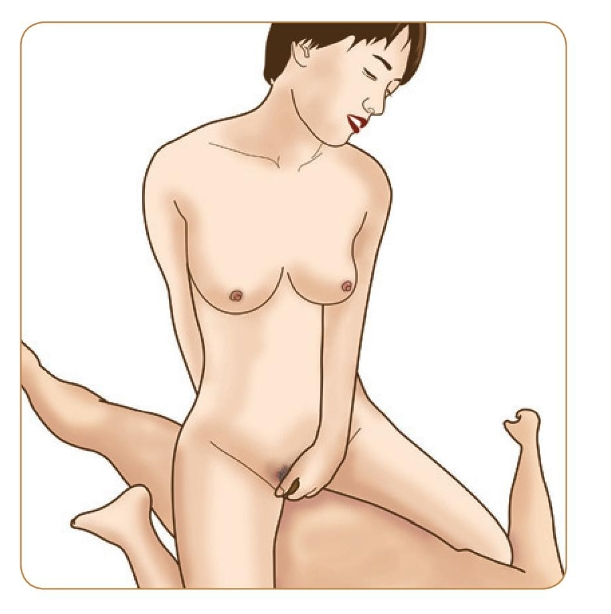
\includegraphics[width=0.7\linewidth]{17}
	\caption{}
	\label{fig:1}
\end{figure}

\begin{figure}[htbp]
	\centering
	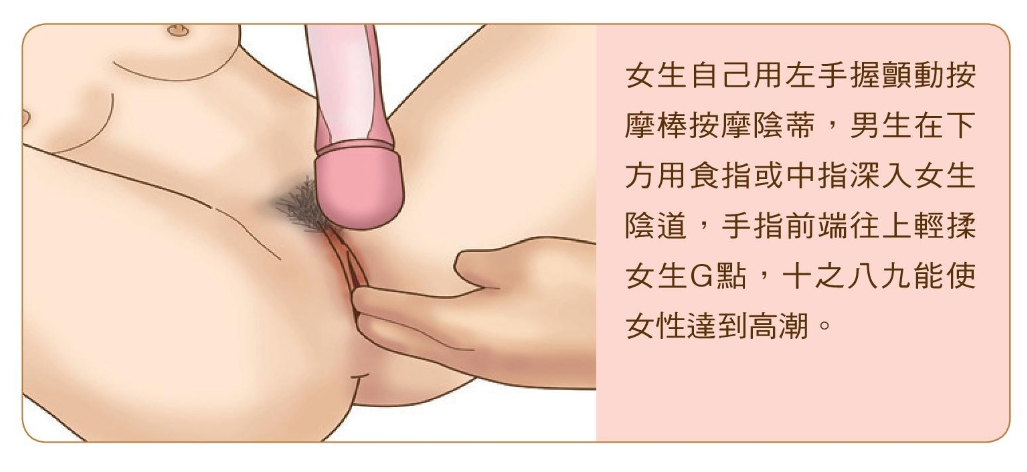
\includegraphics[width=0.7\linewidth]{18}
	\caption{}
	\label{fig:1}
\end{figure}

品玉吹簫说口交
“玉”指女性的阴部,“簫”指男性勃起的阴茎,“品玉吹簫”就是指
口交。这当然是含蓄的说法,其实,口交是完美性爱很重要的一部份,通常
男人帮女人口交是用来作为性交的前戏,让她兴奋,并接近高潮,或是在男
人高潮射精之前,先让女人达到高潮。或许你没尝试过,抑或是你没经验过
甜美的口交,想要试试,以下我就来告诉你一场美好的口交儀式需要具备哪
些要件。

1.要慢慢来:性学博士说:“兴奋时,我们的脑袋会变得很猴急,身体
则会生硬地四处乱摸,以满足当下的生理需求。在欲火焚身的时候,我们的
爱抚像单纯的猥褻,欲求不满的亲吻则淪为劣质爱情小说的描写。”也就是
说,男人这时要留意你不安分的身体的所有动作,对女人抚摸要温柔、要到
位,而不是对着胸部、臀部一阵乱抓乱捏。
2.用一点润滑液:借着润滑液的作用,试着让鼻子滑到她的阴部中心,绕
着圈圈在阴唇边缘滚动,或是像点头一样上下前后滑进滑出。深吸气、让自
己自然的发出声音,让她知道你正在享受这个过程。
3.用力吸:将嘴巴张大,盖住她的整个阴部,往外吸的同时把舌头绕圈
转,并且像吸盘那样,把嘴巴营造成一个真空状态,再用点力吸住她的阴部,
最好趁她还没看着你的时候这样做,因为这个动作看起来似乎不是很优雅。
4.轻揉她的私密部位:用一支手掌掌面抵住她的阴部,像揉麵一样轻揉她
的阴部,这时需要借助大量润滑液。
5.用舌尖挑逗:用你的舌尖去挑弄她的阴唇,在她接近高潮的时候,把你
的舌头从阴蒂头直接往下舔到阴唇系带,同时把你的拇指压在她的阴唇上,
这样才有比较多的肌肤表面可以摩擦来产生快感。

大多数伴侣在进行口交时,被服务的一方多半都平躺在床上,这不只限制
了性爱上的深度连结,千篇一律的动作也会让最火热的性事变得无聊。如果你
要改变这种情况,可以尝试布置不同的情境、尝试不同的角色扮演,或是换一
换做爱的地点,女生甚至可以不需宽衣解带,只需脱下内裤,若地点够隐蔽,
随时都可进行。总之,只要用心,一定能激盪出光热交織的性爱火花。

口交实战技巧
按着步驟来,一次就上手:
1.男性慢慢地把头移到女性的双腿间。
2.持续上下亲吻她的阴蒂,这样可引起她的性兴奋。
3.用舌尖轻柔地舔过她的阴阜、阴唇和阴蒂。
4.让舌尖硬挺一些,重复一次舔过她的敏感带。
5.轻轻地吸吮她的阴蒂,用舌尖绕着整个阴部舔。
6.暂停吸吮的动作,用舌面舔舐阴蒂头。
7.交替用唇舌爱抚她的阴部,直到她达到高潮。

\begin{figure}[htbp]
	\centering
	
\includegraphics[width=0.7\linewidth]{19}
	\caption{}
	\label{fig:1}
\end{figure}

善用口交技巧征服男人
不像女人的阴蒂只像豆子般大小,
男人的阴茎是一支有温度、可伸缩的
肉棒,吃起来很有口感,握着很有手
感,抚摸很有触感。你可以用嘴把他的
龟头含入口中,像吃棒棒糖一样在口中
滚动,也可以用舌头顺着长长的茎部,从冠
状沟开始,像舔冰棒般来回反覆从包皮舔到根
部,也可以用牙齿轻咬勃起坚硬的阴茎,口感绝佳!如果你要让男人印象更
深刻,不妨口中含着温茶水,再把龟头含入口中,缓缓的漱口,男人的心必
定会感受到你给他的无限温暖。
俗話说,“女人经由满足男人的胃,擄获男人的心”,在现今开放的社
会,这已经不流行了,如今多数女人已经不在家煮饭,所以这句話要改成,
“女人经由口交,擄获男人的心”!
美国前总统柯林顿与白宫实習生李文斯基在白宫椭圆形办公室的口交事
件就是举世皆知的例子;已经退休的美国籃壇巨星麥可喬登在球赛中场进化妝室时屢次被多名女性冲进去拉下短裤,瘋狂爭食他的阴茎;歌壇天后瑪丹
娜甚至在电影“真实与挑战”(Truth or Dare)中秀了一段绝佳口技;某位好
萊塢着名女星也曾公开说她喜爱品尝男人的软屌,“屌”就是男人的阴茎。
可以说,天下男人无不喜爱女人为他们口交,女人们,要收服男人,就
放开心尽情享用男人的阴茎吧!
但我也要提醒女人们,男人胯下的佳餚豈止是阴茎,还有两个像滷蛋的
小菜一一睾丸,也是相当美味可口的。当你要享用时,用拇指及食指把阴茎
往上提起,再用舌头舔遍阴囊,这时你的阴道会不知不觉渗出汨汨的爱液,
而男人在此刻早已神飞九霄!

\begin{figure}[htbp]
	\centering
	
\includegraphics[width=0.7\linewidth]{19}
	\caption{}
	\label{fig:1}
\end{figure}

交可以让女人在做爱这件事上和男人主客位互换,要为他进行口交,
女人甚至可以不脱半件衣物,只要动手解开男人的裤头就可以开始,也不必
局限空间,可以在室内或户外,在浴室洗澡时可以玩,在户外任何角落,如
樓梯间转角、郊外樹林中隐蔽处,或是在車上、电影院,只要你把头放低,
埋在男人两腿间即可开动。
趣味小知识
口交算不算性交?
答案是肯定的,口交在法律上算是性交,一方强迫另一方替他口交
算是性侵,而不只是猥褻!若两情相悦而替对方口交就是性交行为。
《史塔报告》透露了美国前总统柯林顿与白宫实習生李文斯基两
人的性关系,包括她多次为这位三军统帥口交的事,柯林顿总统说:
“我没有和那个女人发生性关系!”不过在法律上总统的说法是不成
立的,但该行为若为两愿就不构成犯罪,不过在报告中提到柯林顿想
替李文斯基口交,却因为她当时月经来而被拒绝了,真不凑巧。这个
事件给女人们一个提示:天下男人几乎不会拒绝女人替他口交!
美国没有通姦罪,而我国刑法第10条第5项:称性交者,谓非基
于正当目的所为之下列性侵入行为:1.以性器进入他人之性器、肛门
或口腔,或使之接合之行为。2.以性器以外之其他身体部位或器物进
入他人之性器、肛门,或使之接合之行为。

女人为男人口交这件事完全没有时空限制,不管是在臥房、入住旅店,
当你想要,随时都可以。口交的程序可以由你主动,让男人随你起舞,他绝
对会惊訝且惊喜地拜倒在你灵动的唇舌之下!
女人要主动享受性爱,就从擅用口技、享受口交开始吧!

以下介紹几个常见的口交招式:
嘴唇对阴唇的“传统式”
女人仰臥,两腿张开,建议
用枕头垫高臀部,男人开始轻舔
阴蒂、阴唇、阴道口,接着舌头
伸入阴道浅部伸缩捲绕着舔,这
时你大可闭着眼睛好好享受,但
要提醒你注意以下几件事:
1.专心享受,但要随着男人
舌头转绕自然呻吟、蹙眉,并轻缓的扭动腰身。
2.微微往上挺高你的臀部,就对方的舌头,但是切忌动作太大,否则男人
的舌头会追不上。
3.你必须指引男人舔哪里,力道轻或重,频率快或慢,如果很爽,要高声
惊呼继续,要他舔遍你的阴部!但男人果真认真这样做,不出3分钟,他就会
开始脖子酸痛,脑袋渾沌,如果此时你欲罷不能,不妨用双手扶住他的头,
且把爽叫的音量提高,这对男人有绝佳的激励效果!
4.别让男人的手闲着,提醒男人用食指或中指伸进你的阴道,手指稍微往
上屈,轻抵住G点;或伸入两支手指,中指顶着子宫颈,食指微屈,可触及G
点。

\begin{figure}[htbp]
	\centering
	
\includegraphics[width=0.7\linewidth]{21}
	\caption{}
	\label{fig:1}
\end{figure}

超推荐“骑馬式”
男人躺平,女人面对男
人,跨跪在男人身上,将阴
部对准男人的嘴,男人的头
部最好用小枕头垫高。这叫
“以阴就口”,男人可轻松
恣意品尝美味如生鮮鮑魚的
阴部,这个姿势男人的身体
较不会劳累,所以舌头可以
很灵活的运用,无论阴蒂、
大小阴唇、会阴,都可加长
时间尽情享用,当然,舌头也可不断伸探阴道的深处。
在你尽情享受的同时,男人也别闲着,除了可看着你不断变化表情的
脸,两手别忘向上搓摸你的双乳。

\begin{figure}[htbp]
	\centering
	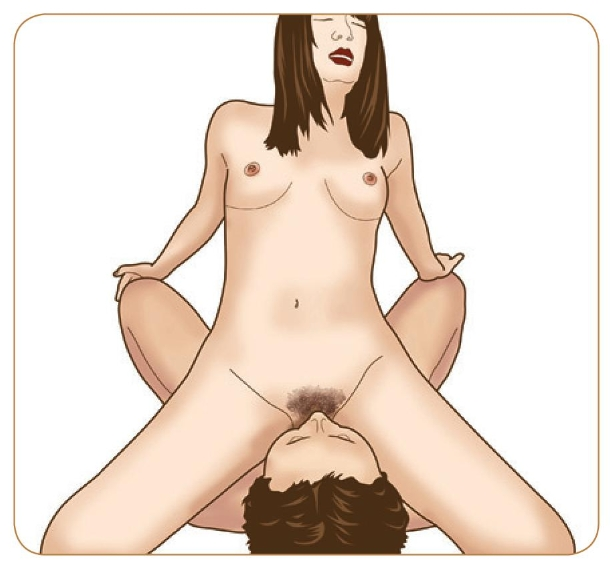
\includegraphics[width=0.7\linewidth]{22}
	\caption{}
	\label{fig:1}
\end{figure}

床(桌)缘式
日常洗澡后,或是假
日的早晨,女人可以很有情
调的在餐桌舖上浴巾,踩上
椅子,自然地躺在餐桌上,
头舒服地垫着枕头,两脚跨
开,把阴部推向桌缘,男人
抓一把椅子,坐到女人如蘭
花展开的阴部前,用手温柔
的把阴唇向两边掰开,开始
用唇舌大啖宛如无花果的阴部,吸吮它的汁液,轻咬阴唇的嫩肉,好似享用一顿精致早餐!这样做的优
点是男人的颈部不会累,且头部及下巴活动不受限制,想吃多久就吃多久。
若想加点特别的,可巧妙的使用身旁的工具,把奶油、果醬、蜂蜜等塗
在阴部,再用舌头去舔食,可以不停变换口味,随意吃个过癮!
再次提醒,过程中你务必让呻吟声尽情表露出来,把快乐传进他的心坎
里。

\begin{figure}[htbp]
	\centering
	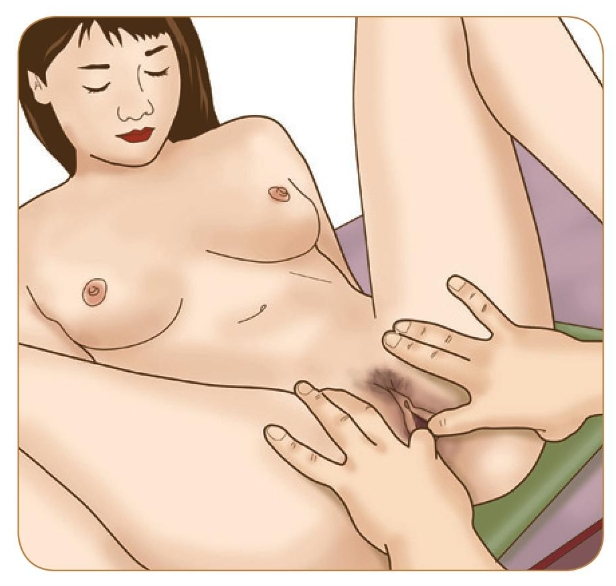
\includegraphics[width=0.7\linewidth]{23}
	\caption{}
	\label{fig:1}
\end{figure}

早餐菜单加点:
女人站立,上身趴在桌面,两腿张开,让男人把你的底裤拉下,掰开你
的双臀,露出两片可口如淡菜的大小阴唇及櫻桃般的阴道小口,加上前端贴
在桌面黝黑如海草的性感阴毛,男人正面坐在矮凳舔食享用,等到女人情欲
高张再高举阴茎插入,享用时别有一番风味。

有问必答
Q:口交会不会传染性病?
A:当然会,而且许多人都是因为
口交而传染上性病。有多种疾病/病原体
都可通过口交传染,如衣原体、梅毒、
淋病、单纯皰疹病毒和HPV等,如果有
以下这些情况,还会增加口腔传染的可
能:牙齦出血、牙齦疾病或口腔健康状
况不佳、口腔溃瘍或生殖器溃瘍等,即
使是受感染的伴侣的尿道球腺液(又名
预射精液)也可能传播疾病,所以,要
避免被传染性病,安全性行为很重要。

男人舔阴技巧大放送:
女人仰躺在床上,先用小枕头把女生臀部垫高,这样做的好处是可以充分
曝露阴蒂的构造,且男人的脖子比较不会酸,过程可以持久些,方法如下:
1.男人伸出舌头,用舌尖快速左右点触阴蒂,好似电动按摩棒,这会激起
女人快速升高的快感,所以称为“舌尖闪电颤动法”,但是用此法男人最多
持续几分钟舌头就累了,所以要接着做以下的步驟!
2.用舌面由阴道口往上贴着前庭舔到阴蒂,重复进行约1分钟,舌头累了再接下一个步驟。
3.嘴巴张开成魚嘴状,覆盖住整个阴部,用舌头在阴道里左右上下舔阴
蒂,约1分钟。
如此由方法1、2、3循环重覆,两人都不会疲累,直到心满意足。
地点可以随机改变,如女人躺在餐桌上、办公桌上,甚至在户外无人
处,可躺在岩石上、汽車引擎盖上,这样做格外有一种紧张的气氛与情趣!

古人的房中术
古人性爱时的爱抚技巧,是从手指尖到肩
膀,足趾尖到大腿,彼此轻缓地爱抚。脚,先从
大拇趾及第二趾开始,而后逐渐向上游移,这是
因为腿部的末梢神经是由上往下分佈的。指,则
由中指开始,接着是食指与无名指,再是三指交
互摩擦。手,先摩擦手背,而后进入掌心,由掌
心向上游移,用四指在手臂内侧专心爱抚,渐渐
上移至肩膀。
手跟脚的爱抚动作完成后,男人的左手就紧抱女子的脊背,右手再向女子的
阴部爱抚,同时进行接吻。接吻也必须依序渐进,先亲脖子,再亲額头。男人也
可以亲吻对方的喉头、颈部和乳头,并用牙齿轻咬耳朵等女人的性感带。
经过上述程序,充分爱抚女子身体的各主要部位后,再慢慢进行“九浅一
深”或“八浅二深”的交合,双方就能得到十分快感。
俗云:“九浅一深,右三左三,摆若鰻行,进若蛭步。”这几个字说的是:
阳具先浅进九次,使女子春意蕩漾,心猿意馬,然后再做很深入的一进,是谓“九浅一深”。因为在九次浅进时,女子能感受温柔摩擦的快感,然后又受到狠命的一进,心动气颤,男人的龟头直抵阴户深处,
女子即刻陷入极度的兴奋状态,阴道发生反覆膨胀
及不断紧缩的现象。
除了“九浅一深”,阳具还需左冲右突,摩擦
女子阴户右边、左边各三次,此时,女子复又感受
到来自阴道两壁不同的快感,使性欲更是高漲,不
能自己。
男人阳具在进出阴道时,不可呆板地一抽一
送,必须像鰻魚游水,橫向摆动身体,以使女子阴
道两壁都能感受到阳具的冲击。或是在进出阴道
时,采用像蛭蟲走路一般,一上一下拱着身体前进。如此女子的阴道上下壁也能
明显感受到阳具抽插的快感,终而神魂顛倒,乐不可支而达到高潮。
九浅一深也好,八浅二深也好,指的都是性交的韻律,同时限制深入的次
数,除非很特殊的情况,女子才需要每次的插入都直抵阴道最深处,因为每次都
深入这种强烈的快感,极易导致性感知觉麻痺,反而弄巧成拙,且若是过于用力
及次数太多,易使女性感觉疼痛。
《玉房秘诀》、《素女经》,及所有性古籍,都主张男人应尽量理智,延后
射精,以配合女子高潮的到来。这种原则,直到今日仍是医界的一致主张,男性若能按上述方法经常鍛煉,必能增强交合的持续力,使夫妻同登欲望之巔

\chapter{性交礼仪}

性交是一件愉快的事,但如果因为一些琐事坏了兴致,真是会令人扼腕,所以,关于性交的一些基本礼仪,不能不知道。

1.事先征求对方同意。

“女人说不要就是要?”那可不见得。有些大男人几杯黄汤下肚,就强迫老婆或女友配合上床办事,完全不管人家愿不愿意。霸王硬上弓的结果,衍生出许多夫妻间的强暴罪,这属于犯罪行为,因此女生若说不要,最好先判断是真拒绝还是说假的,千万别勉强。

2.不可视为理所当然。

虽说夫妻有同居义务,但若对方无意亲热,就该考量可能是时机不对,不妨花点时间取悦对方,比如,女生可以穿上性感内衣,或者喷点香水,男生可以用音乐、美酒来制造美好气氛,让对方心情好转,两情相悦才能让性爱更甜美。

3.尊重对方。

如果今晚你没有性致,不能拖到上床那一刻才宣布“今天休兵”,要对方紧急刹車,这种沟通方式可能会让对方不高兴。若身体真的不舒服,双方可以思考替代方案,比如以口交或情趣用品等方式来替伴侣宣泄,才不会因床事坏了两人的关系。

4.把身体洗干净。

建议性交前先刷牙、洗澡,尤其双脚应该认真刷洗到没有一丝味道为止,阴道及阴部自不待言,女人该将阴道及外阴都清洗到没味道为止,口臭、汗臭、狐臭也都应该先处理,这是卫生问题,即使是平常,女性的阴部、男性的阳具都应保持干净。

5.使用避孕套。

很多年轻人经常换性伴侣,基于安全性行为考量,在新关系开始的前半年内,从事性行为一定要戴避孕套,因为你无法预知你的新伴侣或对方的旧伴侣有没有性病,所以与新伴侣上床半年内或长期使用避孕套是必需的。

6.在乎对方是否快乐。

性交时不可只顾自己是否达到高潮,却疏忽对方的感受,有些行为粗暴的男生,以为女人在床上的叫声愈大愈愉快,有人为此去入珠,其实那是痛而不快,要真心愉快,两人才能幸福长久。

7.勿苛求对方。

不要因为对方一次表现不好,就给她/他贴上标签,严格要求对方与自己同步产生高潮,这样反而会造成双方的压力,要相互体谅,感情好,高潮自然水到渠成。

8.不要比较性伴侣。

千万不要拿前任男友的床上功夫跟现在的伴侣比较。这是伤感情并损自尊的事,也是非常不礼貌的行为,男性若谨记在心,极可能会产生心因性阳萎,损失的是自己。

9.记得赞美对方。

一场美好的性爱后要记得赞美或道谢,告诉他:“你真的好棒,好厉害!”或“谢谢你让我这么舒服”,适时的赞美可鼓励对方让他的表现愈来愈好。

10.保守性伴侣的秘密。

绝对不要公开性伴侣身上的特征,或对他人谈论自己与性侣伴的私密行为,帮对方维护隐私是成熟人格一定要的,若以炫耀的心态向他人述说伴侣的隐私,只会降低自己的品味,让人对你望之却步。

\chapter{情趣用品}

情趣用品也称成人玩具(adult toys)、性玩具(sex toys),是帮助性行为所使用的器具,它对于患有性冷感的女性和性功能障的男性,抑或是中年对性事疲乏的夫妻等,都有改善的效果,也是年轻夫妇、情侣性爱游戏的玩具,能帮助提高性爱情趣、辅助治疗性冷感,简单地说,就是增加性爱情趣的用品。

在性学专家眼里,双方藉由辅助品的帮助来解决生理需求,不但可以DIY不求人,更不会影响或是强迫他人行事;从另一个角度说,它还能为夫妻生活注入情趣,有助爱情更保鮮、更持久。

当人们因为心理、生理等问题无法正常完成性交时,不常以消极的、无做为的熊度来回避这种需求,而是应该借助生殖器之外的身体部位、药物或性用具等来帮助完成性活动。所以,正确使用情趣用品,可以到自慰、自疗的作用。

情趣用品的主要作用:

1.治疗及提高性能力。

2.增加性生活情趣。

3.满足特殊情况下的性需求。

在生殖学上,性病恐惧者、未婚者、长期外出或独居者、性欲较强者或是夫妻性生活未能尽兴时,如男性阳痿、女性性冷淡患者,或夫妻一方有病或致殘而无法进行性生活者,都可借助性器具的刺激来达到性高潮,以获得性满足。

也有人购买性玩具是因为他们想尝试新鲜的性爱花样,在性爱情趣中去发掘自己和伴侣的性潜能,这多与疾病无关,所以,只要不濫用,偶尔使用情趣用品来点刺激,也未曾不可。

现代社会生活节奏越来越快,很多人被工作、生活压得喘不过气,性生活成了可有可无,使得夫妻感情日渐淡去,这时,成人用品的出现很好的改变了这一情况。

成人用品其实有很多种类,如各式自慰用品、情趣内衣、游戏服、跳蛋以及功能性保险套等,在无聊的夜晚,在伴侣没有兴致的时刻,可以扮成温柔护士、狂野海盜、可爱女僕……总有一款能提起他的兴致;或者来个跳蛋,跳蛋是非常好的性爱前戏用具,也是女性朋友自己可单独使用的好玩具,它可以极佳的刺激女性阴蒂等性敏感带,还可选择自己喜欢的频率与强度,让身心快速调整到性爱模式,加快高潮到来,夫妻如果一起使用,还有增添性爱情趣的作用!

由于女性享有在短时间内享受多次高潮的生理特点,所以情趣用品多数都是为女性需求而设计。情趣用品使每个女人在没有性伴侣的情况下,可以利用它享受性快感!它让女人享受性爱可以不必靠男人,不只能满足性自主,且有方便性,包包里放个小玩具,在自己的房间、公室的洗手间,或是百貨公司的五星級厕所,都可以自己来上一段。

情趣用品对身体健康有没有坏处?没有,非但没有坏处,可以舒压、解郁、消火气,对身心健康绝对有益;更好的是,情趣用品不必勉强男人配合,让两性关系更自在。

常见情趣用品依照用途可分为以下几类:

1.阴蒂自慰用。主要是按摩棒、跳蛋,这类用品的功能是能高速震动,目前进化版的跳蛋或按摩棒震动速度有分級,还有各种震动花样,有由弱转强的,或是强弱搭配的,高速震动雖能带来高速刺激,但常会嚇到初使用者。它和自己用手指缓缓按摩不同,但只要多试几次,很快就能学会如何使用。建议使用震动器时最好在隐蒂、阴唇及前庭上塗抹润滑液,不但能增加快感,且能避免因快速摩擦而受到伤害。

2.假阳具。多为长条型与阴茎擬真,使用时放入女性阴道,进階版有电动,可震动、伸缩,甚至旋转龟头,其功能远超过实际阴茎,对女人的阴道做到极尽討好之能事!还有些假阳具在根部多出一段如小指的阴蒂按摩器,在假阴茎插入阴道时透过震动来按摩阴蒂,使阴道及阴蒂能同步达到高潮。

3.乳头震动按摩器。有专门设计罩着两个小乳头的按摩器,但因为有震动功能的跳蛋已经足够用来刺激乳头,大可不必多此一举!

4.加强性刺激类。如龟头冠状沟环(带有突起刺激物的弹性环,固定在头下的冠状沟)、带突起刺激物的保险套(多为硅胶材质,能加大、加长阴茎)等,这些用品的作用都是为了加强对阴道的刺激,使女性更容易达到高潮。

5.润滑剂类。这类情趣用品适合于性兴奋不足、或是绝经期后的女性,它能润滑女性阴道,减少性交的不适及疼痛感,性经验不足、精神过于紧张、难以充分性兴奋的女性也适合使用,它能让女性容易习惯、适应阴茎的插入。

6.情趣内衣。它是内衣的衍生物,重点在于“性感”,透过视觉来达到生理感官的各种刺激,情趣内衣如今已是非常普遍的生活用品。

7. SM用品。如皮鞭、蠟燭、手銬、眼罩等。

有些论点认为女人不要太常使用情趣用品,会因为太刺激而取代对男人的性趣,甚至沉溺其中。我认为这实际上是不会发生的事,试问男人会因为养成了手淫的習惯而裵失和女性性交的欲望吗?不会,这种事从来都没有发生过!

使用情趣用品的时机,往往是在以下几种状况:

1.身边没有男性伴侣,如单身,或是想要享受性爱而不方便找到男人的时候。

2.男人提供的性交无法满足女人的需求,如早泄、不能勃起,或是男人的性技巧不够好,女人无法尽兴时,后续使用跳蛋按摩或假阴茎来满足性欲,这样反而可以帮助男人取悦女人,有益维护两人的性关系及感情,尤其是夫妻关系!所以,女人使用情趣用品并没有沉溺的问题存在,反而有益身心健康,帮助穩定情緒。

男人应该鼓励女人使用情趣用品,除了可用来补救自己体力的不足,还可减轻来自女性性生活需求的压力,甚至可以当成两人性交时的辅助用品,使女人在每一次性活动都很舒服很满意,反而有助提升两人的感情,女人若因此感受到男人对她的体贴、宽容和善意,必然会心存感激。

多年夫妻,或同居多时,有穩定性关系的伴侣,鼓励两人把情趣用品经常摆放在床头,当男人提早射精,女人意猶未尽时,女人可以继续玩到尽兴,不要让男人对你有愧疚!

男人买情趣用品给誰用?女朋友或是老婆?

根据情趣商品业者说,到店里买按摩棒者八成是男人,两成是女人,且近年来购买使用情趣用品的人口有快速增加的趋势。

通常,男人都是单独走进店里,东看西看后再表示要买哪一种按摩棒,店員通常会进一步介紹各种型式的产品,譬如按摩阴蒂的电动跳蛋,或是按摩阴道的假阴茎,假阴茎又分电动及非电动、可伸缩、前段龟头部分可转动等,各式各样。

店老閪看顾客观看的表情和眼种,就可猜出誰是新手谁是老手。如果是新手,他会善意的建议顾客先选择简易型的产品,循序渐进,如果顾客是有使用经验的老手,就介紹他进階版,如可电动兼震动速率可分段、可自动变换方向的假除茎等,有些假阳具根部有可同步高速震动按摩隐蒂的小突出物,让女人阴道与阴蒂同时享受,一阵阵令人无法控制的快感,把女人一步步推向极乐天堂!

业者表示,过去男人购买情趣用品几乎都是给女朋友、情妇或小三使用,目的在討好对方,让女人得到更刺激的性爱享受。从性行为论,这样的用心应该受到肯定。不过最近几年来,越来越多男人表示购买按摩棒是给老婆用!这状况表示,最近男人已经逐渐正面关心和老婆的做爱品质,开始替另一半的性生活快感着想,这是很重要的进步,值得肯定和鼓励!

许多男人不能接受自己的女人,尤其是老婆,在和自己性交时同时使用阴蒂按摩棒,辩称那只是A片的演出,其实单纯是自尊心作崇,因为他不能面对自己性能力不足的真相,或根本忽略了女人欲望的深淵。

何不换个角度想:如果按摩捧可以让A片中的女人兴奋到如痴如醉,为什么不能让自己的女人或老婆享受更高度的性愉悦呢?

如果男人能敞开心胸,做爱时用人工性器,包括按摩棒或是假阴茎,当成做爱的好帮手,让女人每次做爱都能达到高潮,或是趨近高潮,不但可大大减少自己做爱时坚挺持久的压力,且必定会让女人打内心爱死你!成功不一定要自己独力完成,不是吗?

另外,从女性购买情趣用品自娱的人数日渐增加,显示女人性自主意识逐渐抬头;而男人购买情趣用品给女人使用的比例也有增加的趨势,表示男人已渐渐正视且尊重女人的性需求,更懂得如何在性爱中满足女人,这是男女关系的一大进步!

有人担心,若女人使用按摩棒或人工性器成瘾,会不会减低与男人性交的欲望?答案是不会的,女人的性欲和性满足感仍以心理层面为主,男人的阴茎真实插入自己的阴道,和拥抱有温度的男人肉体的满足感,仍旧是人工性器无法取代的,即使是女同性恋人做爱时使用人工性器辅助,也无法取代两人拥抱亲吻舔舐肌肤时具肉体温度的快感。

情趣用品业者透露:经濟越不好,景气越差,按摩棒销售的业绩越好!他们的解讀是:心情越苦闷,经由性爱寻求生活中的小确幸,是最经濟、简便,又最有效率的事!

\chapter{阴毛与腋毛的性感媚力}

在古代,或至少50年前,女人的毛,包括阴毛与腋毛,一直被男人视为不可或缺的性感象征。旧社会时,流传着男人嫖妓嫖到“白虎”会走霉运的说法,而女人被“青龍”嫖到也会有厄运!

什么是“青龍”、“白虎”?

没有阴毛的女人被称为“白虎”,没有阴毛的男人叫“青龍”。常然,上面提到的传言不会是事实,但可以确定的是在当时,阴毛对男人或女人激起性欲有很重要的意义!

如果你曾经看过30年前8釐米的A片影带,见到女主角都是阴毛茂密黝黑,两腋下体毛也是又长又多,也许因为那时的影片是黑白片,所以阴毛及腋毛的性征特别明显,今日再观之,只令人感觉触目惊心,印象深刻。猶记得当年男同学间也是常拿女人的阴毛来討论与分享,当时流行的黄色小书,对女人阴毛是否性感优美、浓密、长短、颜色深浅、形态分佈等,总是极尽描繪之能事!

自从1910年香奈儿在巴黎成立时装店,并开始演变成举辩时装秀来展现季节新装,引領流行时尚历经一世纪,她们由经验归纳出模特儿的选拔原则是:胸部不可以丰满,腋毛必须剃除干净。为什么要如此?因为丰满的乳房及裸露的腋毛这两个性感要素,会转移观眾对服装的注意力。

从此以后,所有出现在公眾面前展示最新时装的女模,皆必须把腋毛剃除,经过时代演变,越来越多女性也自动模仿,当夏天来临前即剃光腋毛理由是穿着无袖上衣露出腋毛会显得不雅观。换个角度想,该是认为腋毛太性感,外露出来给人看不好意思,有些人则不知所以然只是跟着流行。我给女人们一个誠心的建议,别盲目跟随流行,若不是有严重狐臭,建议为了让你在男人眼中更加性感,最好不要剃光腋毛!

我曾经看过一则报导,知名的好莱坞男星布萊德彼特曾说,他喜爱舌舔女人的腋下,因为他觉得女人的腋毛很性感!

回想20世纪60年代中期,比基尼泳装、内衣等轻薄短小的衣着开始在大部分西方国家流行,在健美活动上也十分常见,这虽然风行,但一小块布实在无法把阴部完全遮盖,使得阴毛经常外露,令自己感到难堪,使得日后许多女性干脆把外露在比基尼布料之外的阴毛修剪掉。

近几年来,西方国家的女性开始流行剃除毛的风气,在欧洲裸体模特儿的照片中,常常看到阴毛全部被剃光,也有部分人把毛剃短并做造型。她们会找美容师或是妇产科医师,替她们把阴毛剪成小三角形、心形、长方形,或仅在顶端留下一个小方块等各式造型,煞是有趣!

国内最近有些女性也开始追逐这种流行,到诊所来要求把阴毛全部剃除,问她为什么?得到的答案非常简单:比较衞生。针对个回答,我要告诉你,阴毛的存在和卫生没有关系,只有一种情况是长阴虱,它会躲在阴毛的根部,治疗期间必须把阴毛剃除,在其他正常情况下,阴毛并不会有任何卫生问题。

根据一项非正式的调查,90\%的男人认为看到女人的阴毛会立即产生性欲,并且认为阴毛越浓密越好。所以,奉勤追求性感的你,在剃光阴毛前要三思,因为剃了阴毛即是剃掉了性感,最近甚至还开始流行女人到植发診所植阴毛哩!

关于植阴毛

在东方人眼中,毛发是性感的象征,长出腋毛、阴毛,代表着女性成熟、拥有生育力,但人类约十分之一患有“耻毛缺損症”,即阴部完全没有毛发或较为稀疏的女性,会因此有“发育不全”的信心危机,这问题在医学尚不发达的时代可说是无解,但如今,整型医学发展日新月异,植发(毛)轻轻松松就能完成。而且除了天生的“耻毛缺損症”,现代女性也有纯粹不满意私密部位毛发太细,或对形状、毛发生长方向有意见,希望透过植发(毛)来改善。

探究女性植阴毛背后的原因,终归是考量性交时伴侣的感受,但功能面来看,阴毛可让男女在性交时减少皮肤摩擦,对阴部有保护作用。

告诉你一个有趣的知识

植在阴部的毛从哪里来?答案是:头发,很令你惊訝吧!

你是不是会疑惑:用头发来植除毛,将来是不是会一直长?其实是不会的。植阴毛后的前三个月,种植的阴毛如原来的头发会长,三个月后这些被植入的毛发掉了,自毛根重新长出的则和原生的阴毛完全一样,具有柔软捲曲的毛质,且长到如原有阴毛的长度就不会再长了,很种奇吧!

玩阴毛的无限乐趣

女人的阴毛可以有很多种玩法,每一种都可以让男人神魂颠倒。比如洗澡时用泡沫抹在黝黑柔软的阴毛,让它看起来好像黑色漩涡,十足性感!或是在性爱高潮后,让男人用梳子帮你梳理阴毛;睡前可以要男人用润滑液塗抹在你的阴毛,让烏黑的阴毛如羽毛散开,平贴在白皙的下腹;也可以要男人用吹风机把你的阴毛吹得四散飄逸,这等性感和情趣,一定会让男人倾倒。

看截至目前日本和韓国的A片,演員全都保留完整的阴毛,一丝未刮除,美国和欧洲最近的A片则大部分将阴毛剃光,有些则刮除部分或经过修剪,但西方的A片会特别把镜头聚焦在隐蒂,把阴唇翻开,外露阴道的肉体。我认为,少去阴毛的魅力,把埋藏在里面的秘密赤裸的展现出来,成了另外一种不必要。试想,如果阴毛不见了,日后合法的A片就没必要再在第三点打上馬赛克了。

比基尼线

指女性在穿上比基尼泳裤后,泳裤下方两侧与皮肤交界的线。由于女性阴部正常的毛发生长常会使阴毛露出在比基尼泳裤之外,为了避免露毛的尴尬,于是整型医学兴起了“比基尼线除毛”,常见的方式有:

1.美式:仅除去露出在泳裤外部的阴毛,以这种款式脱毛后,所剩阴毛形状为倒三角形,又称“倒三角式”。

2.法式:完全去除包括阴唇在内的毛髪,仅在外阴上方留下一条约4公分宽的垂直带(被戏称为“飞机跑道”,或“花花公子带”),这种脱毛方式在那些必须穿着襠部区域非常窄的衣着的模特儿行业中很流行。

3.巴西式:指去除盆骨区正面和背面的所有毛发,用于穿着丁字裤的人。此式脱毛能使成年女性看上去像女孩,在性行业中颇为流行,但这种脱毛方式不自然,且免疫系统差的人在施作过程中会有感染的风险。

\chapter{前戏}

前戏要怎么进行?

1.发动温柔攻势:我们不妨将男女的身体当成乐器,男性在弹奏女体时,請轻捻慢揉,温柔以待。女性需要情緒和精神上双重的爱抚与逗弄才能挑起情欲,所以請男士们放慢速度,手口并用,亲吻爱抚她的身体,从最远的肢体向胸乳及阴蒂等重点部位慢慢接近。

<<<<<<< HEAD
2.吻她/他千遍都不厌倦:親吻是最普遍的前戏,两性都需要伴侣主动、温柔的探索他们的身体,男人除了可親吻唇舌、耳垂、脖子、背部、乳头、会阴、阴蒂等一般人熟知的敏感部位之外,也别忽略手指、脚趾、腋窝、大腿内侧、手肘及膝關节内侧等部位,可尝试舔舐、吸吮、轻咬等方式,能激起女伴不同的反应;女人也可以反过来做出和男人一样的动作,主动去探索他的身体。
=======
2.吻她/他千遍都不厌倦:亲吻是最普遍的前戏,两性都需要伴侣主动、温柔的探索他们的身体,男人除了可亲吻唇舌、耳垂、脖子、背部、乳头、会阴、阴蒂等一般人熟知的敏感部位之外,也别忽略手指、脚趾、腋窝、大腿内侧、手肘及膝关节内侧等部位,可尝试舔舐、吸吮、轻咬等方式,能激起女伴不同的反应;女人也可以反过来做出和男人一样的动作,主动去探索他的身体。
>>>>>>> 5ab1aa26d2f60189e2188622658785c9dc1de2d6

3.动口也动手:在这个亲密时刻,千万别让手闲着,用指腹轻轻抚摸、用指尖转圈圈、指头轻轻按压等变化多端的“指技”,可运用在所有能想像到的和有待开发的敏感带上;同时,别忘了拥抱是最简单的亲密接触,它每每能使男性汗毛豎起,心跳加速。在亲吻的同时,女人可以动手探索男人的下体,主动抓住男人的手,引导他的手来到你的阴部,他肯定会受寵若惊。

4.尽情驰骋性幻想:女生可以藉由自慰探索自己的敏感带,因为这时候你可以无所限制,如果你想要請周湯豪、金城武、李敏鎬等男神来出任虛擬男主角,也没什么不可以?而这也证明大脑是最重要的性器官,因为高潮不仅源自生理反应,也来自心理感觉,不过虛擬男主角最好是遥不可及的人物,若你幻想的是闺密的男朋友,那就是精神出轨喔!

5.享受性交前高潮:男生也可以用女生自慰的方式帮她自慰,让她在前戏时达到第一次高潮,这不但能延长性交的时间,也能使女生在性爱活动中享受多次高潮。

6.抓准时机停止前戏:何时該停止前戏呢?从女生咬嘴唇、挥舞双手、扭动身体、双腿及阴部的收放、急促的喘息、分泌的爱液,都可得知这时就該停止前戏,开始办正事,此时的享受真是一刻值千金。


\chapter{姿势}

\section{女上男下}

这是女人不能错过的做爱体位,极力推荐这种性交姿势,因为这才是女人能够真正主控性交过程的姿势,让自己满足且能随心所欲。

女人坐在男人身上做爱的好处,首先是可以“把男人的阴茎整支没入阴道”,那种饱足实在的快感,绝非言语所能形容。

\subsection{招式1:前后扭动}

两膝外张,两腿放松,可以把全部重量直接坐实在男人身上。

1.以一前一后的方向扭动,这时阴道的表面紧贴包覆着雄壮坚挺的阴茎,阴道每一寸肌肤、每一个细胞,都深刻感受到阴茎的温热,那样的享受自不待言!

2.先缓缓的前后挪动,试着让阴茎摩擦阴道前壁并停驻在G点片刻,像是吞入整根热狗但暂不嚼它。

3.让阴道紧含着阴茎,吸它的美味,享受口感。动作的方向,可时而做圆周回转,时而上下抽送,速度或快或慢,全凭心意调节变化。

4.女生在上位可随己意在男人的耻骨上前后磨蹭阴蒂,这种美妙的感觉胜过自己用手指按摩,尤其此刻能兼有阴道及阴蒂同步产生的快感,这是你单独一个人做不到的,因为只有当男人直挺的阴茎插进你的阴道里,才能达到此境地。

5.当你面对着男人,男人可以逸待劳,无疑是对他最好的体贴,男人可以观看你销魂享乐的表情,欣赏你晃动的双乳,对他而言是极为刺激的情趣!

6.你的臀部前后挺退的频率,可随着快感逐渐升高而自动加快速度,不断上升直到高潮喷出!

7.男人的阴茎一柱擎天,龟头可直抵子宫颈,给你带来很具体的感受。

关键技巧:女性下体摆动的方向、力道轻重、速度快慢、深浅,可随自己的意,更能恰到好处触及阴道的痒处,包括按摩G点。这是女人在玩阴茎,且充分按照自己的快感需要随心所欲。这样的玩法如果是男人在上位,由男人主动抽送,无论他多么努力、技巧多好、如何用心,绝对是做不到的!

\begin{figure}[htbp]
	\centering
	
\includegraphics[width=0.7\linewidth]{24}
	\caption{}
	\label{fig:1}
\end{figure}

\subsection{招式2:上下抽送}

女生在上位,两膝张开,蹲跨在男生的阴部上,主动抬起屁股上下抽送男人的阴茎。女人坐在上位除了如“技巧1”前后扭动之外,也可主动抽送,深、浅、快、慢、轻、重由你决定,可精准地搔到自己的痒处;或是你可以尝试改变方向,采取背向男人坐在他身上的方式。

无论前后推扭,或上下抽插,可以面对男人,也可背对男人,两种方式都可边性交边用手指抚弄男人的睾丸,会让自己更兴奋。

\begin{figure}[htbp]
	\centering
	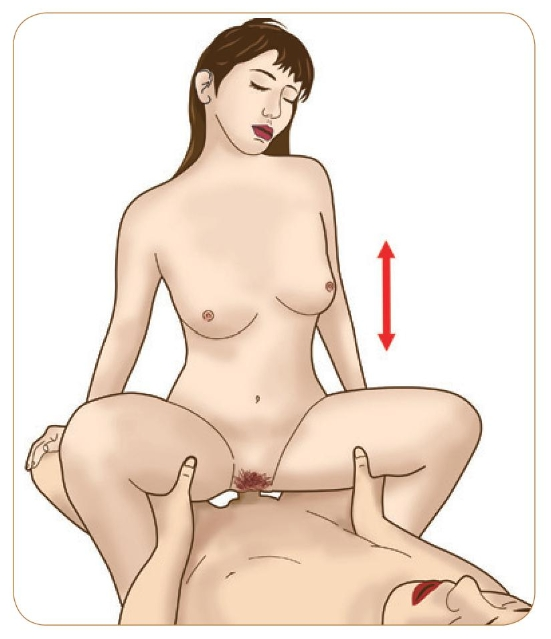
\includegraphics[width=0.7\linewidth]{25}
	\caption{}
	\label{fig:1}
\end{figure}

背向式关键技巧:

两膝张开,背对男人,挺身坐在他的耻骨上把臀部前后推动,此时阴茎偏重抽动阴道前壁,紧紧压住G点,快感不言可喻。可以一手扶住男人的膝盖,一手抚摸他的阴囊,饶富趣味。

侧转式关键技巧:

坐在男生身上,向左/右侧转90度左侧坐,两脚跨开,把男人的左脚放在你的两腿间,扭动抽送;再改换右侧坐,方法相同。你会发现,同样的动作只是转换不同的方向,会使阴茎碰触的角度不同,感受千遍万化。

\subsection{招式3:坐在男人耻骨上身体前倾或后仰}

你坐在上面,身体可以向前倾,这时龟头会把子宫颈向后顶,硬挺的阴茎可施压摩擦阴道后壁,饶富趣味!

也可以换成身体后仰,这时硬挺的阴茎整个压迫在阴道前壁,顶住G点,可恣意地抽动扭拐,保证让你爽到极点!

特别提醒你:

别把阴蒂冷落在一旁!

你要好好利用他的双手,不要让它们闲着。你可以把他的右手拉到你的胯下,反手垫在他的耻骨上,这么一来,每一次你撞击男人的当下,你的阴蒂就在男人的指尖摩擦一次,如同同步手淫阴蒂一回,一举两得,很不错是吧!

\begin{figure}[htbp]
	\centering
	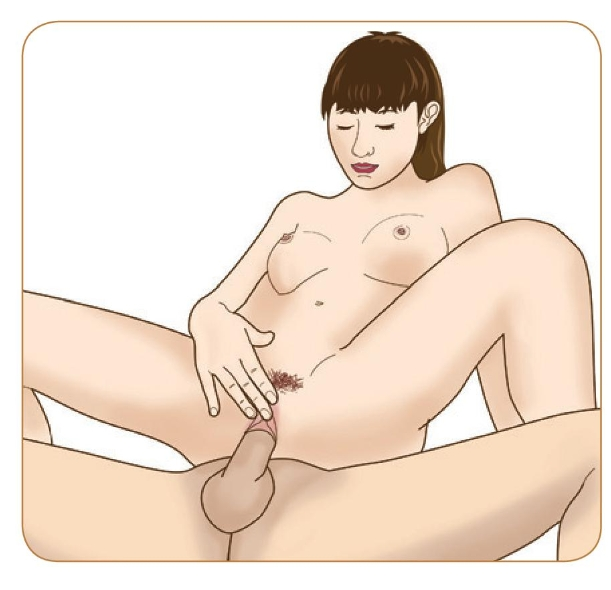
\includegraphics[width=0.7\linewidth]{26}
	\caption{}
	\label{fig:1}
\end{figure}

关键技巧:

你知道为什么每一种姿势我都教你要把身体换个方向,同样的动作再来一次吗?那是因为男人的阴茎不像热狗,不是笔直光滑头尾围径一致,360度都长一样,事实上,阴茎的龟头稍扁,阴茎干呈香蕉状弧度微弯,所以只要转个方向,阴道的感觉就会截然不同,快感也大大不同。

女人主动“骑”男人的优点

做爱时采坐姿是女人“骑”男人,躺着是“被骑”,而女人“骑”男人的优点包括:

1.男人躺平,以逸待劳,可以比较持久不射。

2.男人可以欣赏女人陶醉的表情,此刻的表情最美,会让男人惊奇的发现女人内心深处潜藏的欲念,激起他更炽烈的性欲!这情境会常留在男人心中,使你成为他每次想做爱时的首选对象,且长久延续与你做爱的热情。

3.女人可以把男人的阴茎整根没入阴道,做爱节奏可以完全依照你的需求,或抽、或扭、或转,深浅、速度、力道,全视你的需要调整。

4.好似搔痒,你自己来绝对可以搔到痒处,抓到尽兴为止!如果男人在上位,好像要他人替你抓后背的痒,你说左说右,费尽口舌,终究很难随心所欲!

\section{男上女下}

\subsection{正面插入式}

人类是唯一可以面对面做爱的脊椎动物,可喜。但采取这种做爱方式时,在下位的人记得要善用枕头。无论在任何情况,第一个动作记得顺手把枕头抓过来垫在臀部。

男上女下正面插入式有以下几个好处:

1.把女性阴部如蘭花綻放般完全呈现,表露在男生面前,两片肥厚且较深
色的大阴唇,边緣充满皺褶如蘭花瓣,阴蒂如花蕊,层层叠叠完全攤开,让
人饱覽无遗,男人看了誰不心动!
2.男人的阴茎可以顺利插入,而龟头滑动的路径偏重阴道前壁,频频在G
点附近摩擦,一开始即有快感,女人可以很快进入快感高原期。
3.可以相互看到对方享乐的表情,这是莫大的喜悦。
4.男人在抽送阴茎的同时,可用手指轻轻撩拨按摩她的阴蒂。女人应该
用手指把阴蒂的包皮往上稍微提拉,使阴蒂头充分突出外露,让男人轻触按
摩,做爱时千万别冷落阴蒂一分一秒!

我还要教男士一个重要技巧:将右手大拇指指腹轻轻放在女人的阴蒂
上,然后把前臂固定贴在下腹部,当你往前推送阴茎时,小腹同时推动前
好女孩也该享受狂野的
臂,把你的大拇指也往前推动按摩伴侣的阴蒂,抽出时顺势把指腹往后撤,
如此一抽一送,使指腹一前一后揉搓阴蒂,女人可同步享受阴蒂加阴道的双
重快感,很快就能把女人推向高潮!(如下图)男人这样做既有效果又省
力,且可以持续不停直达高潮。
这个方法类似假阳具前通常有一个突出物,可以在假阳具插入时产生震
动以刺激阴蒂,不过我提供的方法更自然,能给女人更好的享受。

再次提醒你,任何一次性交,绝对不能忽略爱抚阴蒂!
你应该告訴男人的秘密:在性交过程中,要让女人达到高潮,男人最
大的武器不是阴茎,而是耻骨。让男人用耻骨碰撞你的阴阜,就是微微隆起
长阴毛的地方,耻骨压迫,摩擦阴核,会使女人在阴茎插入的同时升高兴奋
度,更快达到高潮!所以在两人性器接合后,男人就要以耻骨压迫阴核的包
皮,巧妙的刺激阴核,努力碰触阴阜,让她更快乐。
同样的,女人骑坐在男人身上时,不管方向如何转,角度都要随之调
整,让你的阴阜顶住男人的耻骨,让他的抽送动作时时摩擦你的阴蒂,好似
在手淫时能同步享受阴道及阴蒂的高潮!

\begin{figure}[htbp]
	\centering
	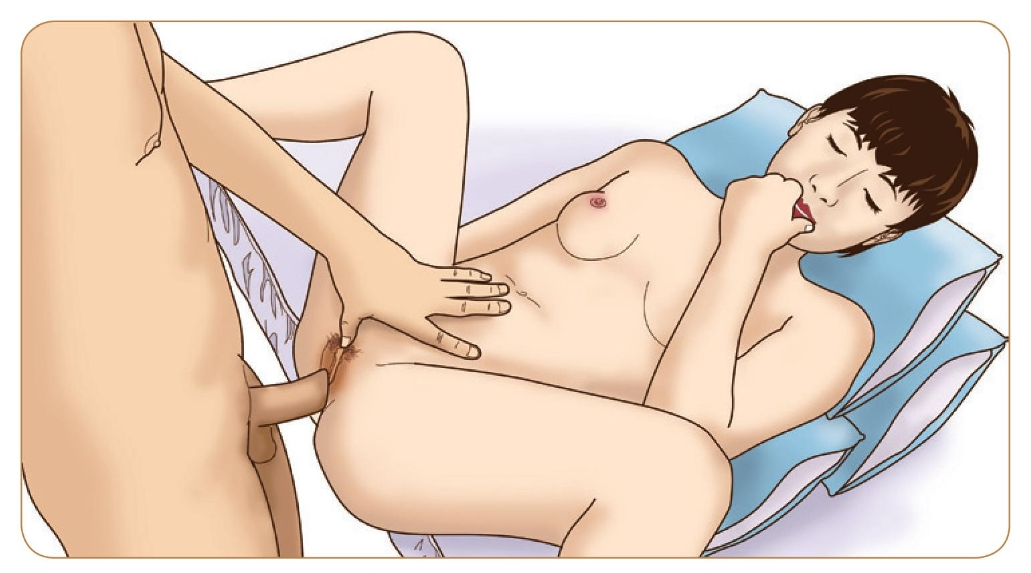
\includegraphics[width=0.7\linewidth]{27}
	\caption{}
	\label{fig:1}
\end{figure}

\subsection{男上女下,传统体位式}

这是个简单易行且有创意的做爱方法,这招不必我教,是很自然大家都
会的姿势,但我要告訴你的是,如何運用这个平凡的姿势做各种变化,使性
交不会淪为例行公事,日久失去激情。

\begin{figure}[htbp]
	\centering
	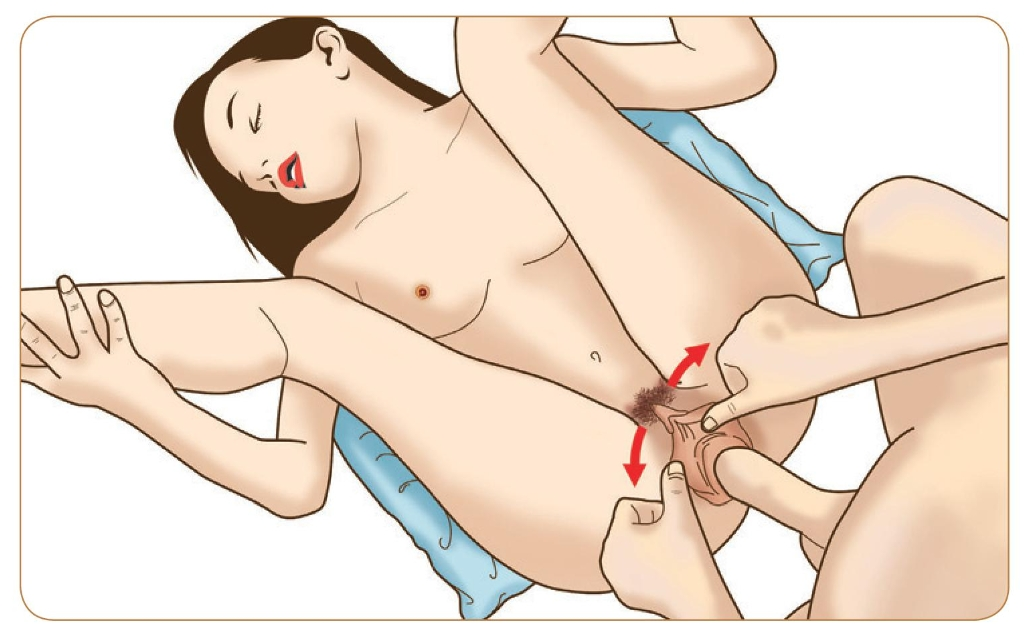
\includegraphics[width=0.7\linewidth]{28}
	\caption{}
	\label{fig:1}
\end{figure}

首先,你必須先把姿势调整好:
1.把臀部垫高到男人阴茎插入最适当的高度。
2.两膝弯曲,尽量向外张开,两手从外绕过大腿,同时把臀部向两边掰
开,充分暴露阴部,让他可以轻易地长驱直入,男人在此性欲高漲之际,一
定会对你的体贴感激涕零。
以这个姿势做爱,不必老是躺在床上做,你可以在男人抽送一阵子后,
主动建议把位置移至床緣,这时男人可以改成站姿,这样比较省力气,如果
射精在即,也可以延缓射精。

这个招式的基本动作为:女生的臀部垫枕头,双腿向外展,男人面对女
人站立,双手扶住女生的膝盖,交合时可有以下的招式变换:

\begin{figure}[htbp]
	\centering
	
\includegraphics[width=0.7\linewidth]{29}
	\caption{}
	\label{fig:1}
\end{figure}

\begin{figure}[htbp]
	\centering
	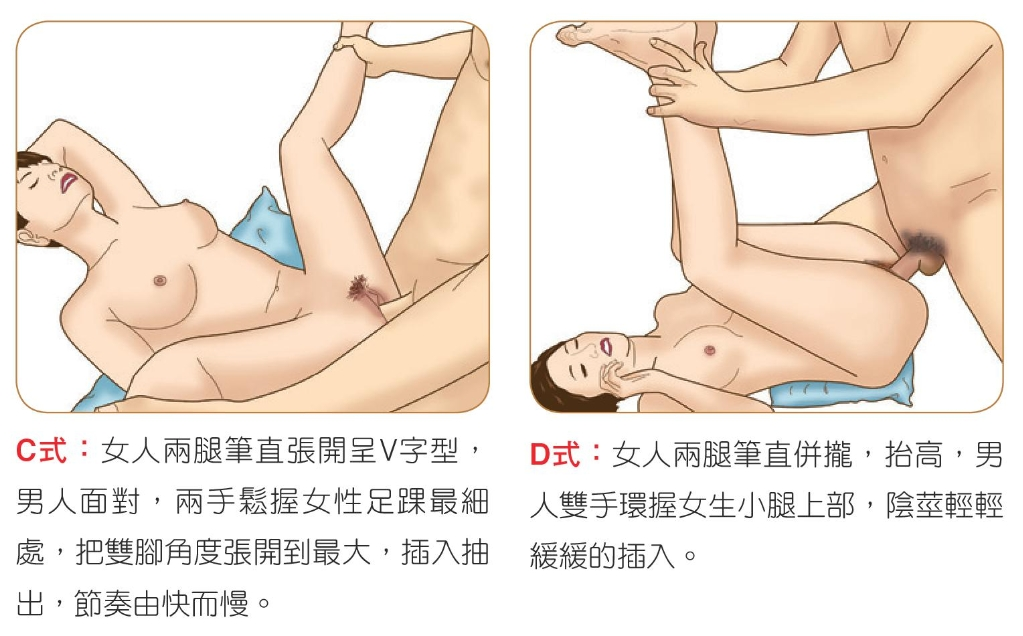
\includegraphics[width=0.7\linewidth]{30}
	\caption{}
	\label{fig:1}
\end{figure}

这个招式的关键技巧,说明如下:
1.女人阴道有紧抱阴茎的实体感,因为紧,所以动作宜慢,每一次插入深
入到底,可直顶到子宫颈。
2.男人面对女人站定不动作,女人双腿仍然并拢,但双膝可以稍微弯屈,
双脚脚底板平踩在男人胸部,脚掌顶着用力,女人臀部主动往上抬,阴道含
着长又硬的阴茎,不爽也难!
3.相对位置不变,女人右腿向右伸直平贴在床緣,左脚垂直朝天,两脚呈
L型,男人抱着一条修长美腿,阴茎平行插入,会非常滑顺,可以长驱直入,
每插至最深处,龟头碰触子宫颈那一刻,激情的快感会让女人觉得心脏像是
要从口中跳出一样,必定使她惊呼连连。
4.相对位置不变,女人改成右脚垂直朝天高举,左脚平放,男人站立,用
右手抱住小腿,阴茎轻缓地插入又抽出,左手大拇指指腹轻按在她的阴蒂,
跟随阴茎插入抽出的节奏按摩阴蒂,男人可欣赏女人脸上销魂的表情,女人
則可領受最高品質的性爱。

\begin{figure}[htbp]
	\centering
	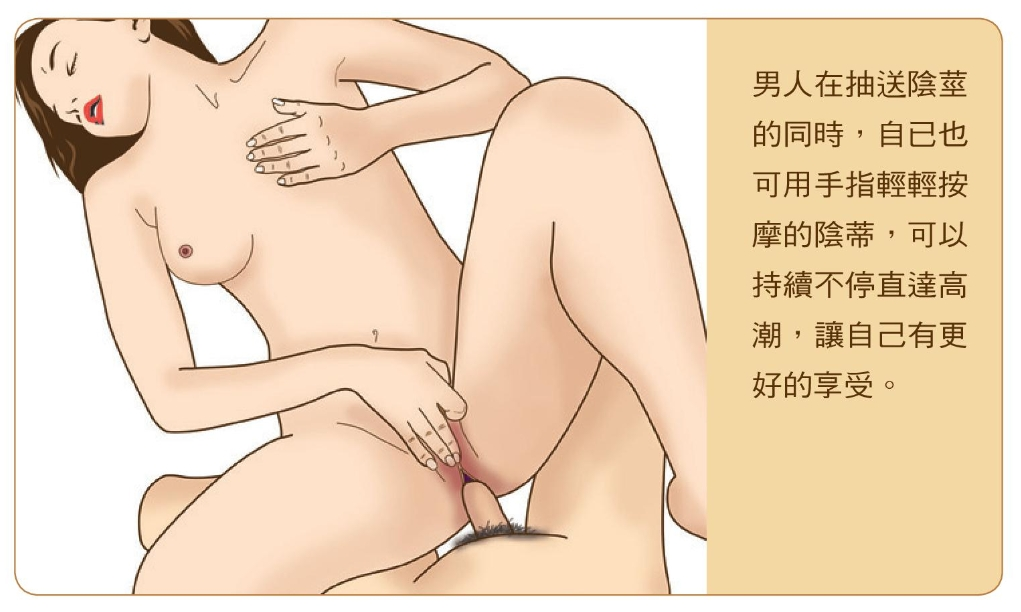
\includegraphics[width=0.7\linewidth]{31}
	\caption{}
	\label{fig:1}
\end{figure}

这个招式的优点:
1.阴茎插入的角度让龟头摩擦的重点在阴道前壁,没有停歇的连续刺激G
点,让女性的激情很快上升到最高点,一直維持在快感高原期。
2.每次抽送阴茎,男人的耻骨充分撞击裸露外现的阴蒂,一次接着一次,
把女人很快推向高潮。
3.男人阴茎的根部刚好卡在女人阴道后壁出口及会阴,不会摩擦到尿道
,阴茎抽送再久、次数再多,都不会造成尿道疼痛發炎。
4.女生把屁股垫高,会使子宮朝腹腔往后陷入,把阴道拉长变窄,宛如
一道长廊,可增长1/3的阴道深度,缩小1/2的阴道宽度,且使阴道表面积增加
1/3,整个性交快感指数至少飆升三倍。
5.男人阴茎没入阴道时有无限暢快的感觉,女人有一口含入整支美味香肠
的满足,阴茎每次顶至尽头,女人的心脏就有如欲从口中冲出一回的快感!
再次提醒,做爱时别忘了身边最简单好用的情趣用品一一枕头。

枕头的妙用
男上女下时,拿枕头垫在女生臀部,
女生两膝尽量向外张,充份露出阴部,大小
阴唇、阴蒂、阴毛全都如蘭花綻放,层次
分明,历历在目,阴道口也微微张开,
阴道皺褶若隐若现,令男人垂涎欲滴。这时,男人可趴下先用舌头舔食一
顿生鮮美味,品尝汩汩渗出的淫水瓊汁,而后再提起早已漲到欲爆裂的阴
茎,毫无阻力便能顺暢插入淫液已充分润滑的阴道,两人即可进行一场欲
死欲活的拼斗!

\subsection{剪刀式}

这也是性交时常見的体位,不管两人是面向、同向,或两人是头脚同
向、头脚反向,都可以,随你们喜欢。
招式1
女人右侧躺,左脚举起放轻鬆,男人把女人的左脚轻轻握着,举高,把
自己的脚跨跪在女人左大腿的两侧,这样能使阴茎很容易插入女性的阴道。
这个姿勢的優点在于,不論女人的阴道口朝哪一个方向,阴茎的角度都
可以自在调整,让整个阴茎沒入阴道,男人的大腿根部則在每一次抽送都会
撞击女性的阴蒂;也可以右手扶着女性的腿,邊抽送时邊以左手大拇指按摩
阴蒂。男人此时可以观賞女人欢愉的表情,会越加兴奋!

招式2
女性維持以上侧躺姿勢,屈膝,阴茎轉个角度从背后插入,每插入一
,女人的心脏就如同被撞向口中一次,够刺激吧!
招式3
上一个姿勢告一段落后,再轉向左侧躺,女人抬起右腿,男人抱着抬起
的腿繼续插抽,很奇妙的,女人的感受与躺右侧时完全不一样,是种全新的
快感!
关鍵技巧:交合时男人把女人的腿往上抬高并拉直,阴道的感觉与把膝
蓋弯曲的姿勢又有所不同。

最自然的姿勢,从背后插入
人类真是神奇!所有生活在陸地的脊椎动物,性交时都是从背后插入,
包括羚羊、斑馬、狗、猩猩、人猿等,人类是陸地上唯一可以面对面做爱的
哺乳动物。
此外,女人也是唯一可以天天做爱的雌性脊椎动物,其他的雌性动物只
有在固定的發情期间才会接受雄性的性交邀請。在發情的这段期间,雌性动
物会發散出味道能远播千里的濃烈荷尔蒙,雄性动物闻到气味时,才会追逐
并与之交配,其他时间,雄性动物不会主动找未發情的雌性动物性交!
由此可見,上帝是何等地寵爱女人!因此,就动物生殖的天性而論,
从背后插入式性交其實是物种最本能的姿勢,甚且我还要告訴各位,性交时
从背后插入是最合乎生理构造的正确姿勢。理由是,女性阴道的直线和脊椎的直线呈现锐角,采取从背后插入式性交,当女人趴着張开双腿,阴道的方
向与男人在后面阴茎往上翹起来的角度刚好平行,好比长劍入鞘,能长驱直
入,毫无阻碍。
以这种方式性交,绝对不会因為角度問题过度摩擦女性尿道口而造成蜜
月病(新婚时因性交頻繁,女性尿道口过度摩擦造成的尿道發炎)。所以,
当男人突然性欲大發,而你毫无心理准備时,可以趴下,把阴道口塗满润滑
液,然后把阴茎当成按摩棒,把性交当成舒服的阴道按摩,经过几次抽送暖
身之后,很快就会產生性快感,点燃欲火,加入战局;或是,当男人从正面
抽送一阵子后你仍然达不到高潮,可以翻身要男人从后面插入。以下介紹几
个性交时从背后插入的关鍵技巧:
1.洗澡完后,男人坐在沙發上看电视,你可以悄悄靠过去,跪在沙發上,
臀部朝向男人,让男人坐着,用手把你的两片大阴唇掰开,让他舔食你的阴
道、阴蒂、阴唇,也可以让他用食指或中指伸入阴道,自然弯曲轻扣G点,让
你為之銷魂。
2.当阴茎勃起时,男人立即站起来,让阴茎笔直插入阴道,在阴茎插入的
当下,你会倒吸一口气,简直爽斃了!
3.两人轉換体位。男人仰身躺坐,女人坐在男人的阴茎上,两人同向,女人双足踩地,可以前后扭动、左右摇摆,也可以抬起屁股上下抽动,享受激
情!
4.当男人口中有酒气让你不舒服,但他又欲火焚身时,你可以主动跪趴
下,让男人从背后插入。
这个招式的優点:
1.男人从女人背后口交舔阴的優点是可采坐姿,时间久了脖子也不会酸,
且轉舔各方向都格外灵活。舔阴时要把阴唇尽量掰开,使舌头能更深入阴
道,舌头舔的走向和从正面时相反,給女人的爽快感觉也不同。
2.阴茎可以整根都插入阴道,女人会感觉阴茎特別长,特別爽。

蜜月期从后面插入
可避免尿道炎
其實「蜜月病」不是单指新婚初期,应当包括「性交頻繁期」,因
為頻繁性交摩擦阴道及尿道口会造成尿道發炎,尿道炎的症状為排尿疼
痛、排尿困难、頻尿、血尿、轻微發烧、畏寒、全身倦怠。
造成的原因是尿道夾在阴道和恥骨中间,恥骨是硬的,男性从上位
正面插入会把尿道夾在中间摩擦,容易红肿破皮。若从后方插入阴道,
阴茎进出的摩擦着重在阴道口的后部,压力会轉向会阴及肛門,这里的

组织柔软有彈性,且因為角度的关系,阴茎进出时不会卡在尿道口摩
擦,大大减少尿道炎發生的情況。

特别提醒:
1.你可以先把内褲脱掉,撩起裙子,把臀部抬高,胸部趴在椅背,两脚跨
开,两手往后把双臀掰开,露出毛絨絨如熟透爆开的无花果,男人此时绝对
是見獵心喜。
2.我建議男人先用手技替女人暖身,用食指及中指,微曲轮流探入阴道,
挑逗G点,或在阴道口用手指绕着圈轉,或轻轻抚弄她的阴蒂,再起身站立,
把挺直的阴茎轻轻地推进阴道,先浅后深,先缓后急。
3.在做爱的过程中,你可以是導演、主角兼编劇,所以你千萬要随着男人
抽送的深浅、快慢节奏,惊呼出声,与男人的动作相呼应!你必須要把握整
个做爱的过程,用心掌握节奏,藉由吟叫的音量大小、音韻高低,好似电影
的配乐,来誘導劇情的鋪陈!
4.性交时若是采背后插入式,我建議女性还是趴跪在床緣比较理想,因
為如果两人皆趴跪在床上,两人的腿长短不同,
若女人的腿短、阴道口低,男人腿长、阴茎
高,姿勢会对不上,做起来很不順暢。若
女人跪在末緣,男人站立,男人的阴
茎可以调整高低,且男人站
立时使用髋关节和膝蓋
两个关节推动抽送,不
但姿勢變化的弧度加
大,也可以更加持久
不累!

再教你一个小绝招:
男人用两手把女人两邊臀部向外掰开,再行插入抽出的动作,此时阴道
]被拉成扁圓状,而被压扁的阴道前后壁夾住进出的阴茎,是另外一种超绝
的爽!
如果是站立,則女性張开双腿,上身趴在书桌或餐桌,或廚房的流理
台,都是很理想的地点,其他技巧同上。
在車内,男人坐在座椅上,女人叠坐在男人身上插入也是很好的姿勢,
但开始时男人先把女人双臀往外掰开是必要的动作!
有問必答
Q:身高较高的男人阴茎也比较长,对吗?
A:錯,男人的阴茎和身高归不同的基因管,
是单獨的遗传因素,就好比女人胸部的罩杯和身高
不相干,不是身材高大的女生乳房罩杯就比较大,
相反的,有許多身材矮小的女性是D罩杯,也经常
見到許多身材高大的女性是扁平胸部!
但阴茎的长短和种族是有关系的,譬如白种人的阴茎平均长度為15
~25公分,黑种人平均也有20公分以上,黄种人平均為10~15公分;
至于粗細,則大抵是越长者相对粗一点。
阴茎长度超过15公分其實对女人性交快感并沒有太大帮助,因為阴
茎较长者通常比较软,且性交时一段阴茎留在阴道外面,不能全根尽沒
入,性交时反而缺乏男人恥骨碰撞女人阴蒂的快感!

两人共浴,洗澡兼享乐
洗澡是每个人一天中身体最放鬆,心情最舒坦的时刻,女人怎能錯过每
天这个最好貼近男人的时刻呢?
日本人一直有男女共浴的传统,这是值得学習的。一般而言,日本女性
的身材不是特別火辣,肉体卻是特別性感,性生活自古特別精采,这与她们
習慣与男人共浴的習俗有绝对的关系!
羨慕吗?其實你也可以。每天你都有一次这样的機会,把你性感雪白的
身体裸露在男人面前,这是让男人很自然对你垂涎產生性欲的機会,何乐而
不為?心理学大师佛洛依德認為,任何感情皆起因于性的冲动,而人们每天
都有一次让双方自然点燃一次欲火,也為相互间感情添加柴火增溫的機会,
不是男女之间最美好的事情吗!
女人的肉体在水中顯得特別細嫩白晰,任何一处皆令人感觉可口欲食,
其實男人的肉体不也是一样。女人淋浴时,水珠成串汨汨自雪白的頸項延着
乳房流到肚臍,再流经黝黑的阴毛,延着毛尖如溪流、如雨滴,男人看了必
然情不自禁想把唇舌貼在你的乳房,舔吮你的乳头,蹲下来吸食如生鮮鮑魚
的阴唇及阴蒂,你当然也可以恣意舔食男人的阴囊,大口吞食他的阴茎!
关鍵技巧:
1.每天替男人的阴茎抹香皂是你特有的权利,把他的阳物当成你的小寵
物,溫柔的清洗阴毛,順手把玩它,亲吻它,吃它。
2.也授权給你的男人,替你全身抹上香皂,你的肩頸、乳房、背部及臀
部,最重要的当然是阴毛、阴唇、阴道前庭,男人必須仔細轻柔翻开清洗,
他有权利順勢用唇舌舔食享用一番!
沐浴时,不管是在浴缸泡澡,或用花灑淋浴,都是很美很性感的事情。
如果你爱这个男人,乐于和她共享性爱,快点把两人共浴變成每天类似宗教
禱告的必要儀式吧!

Q:阴茎的长、短、粗、細,哪种做爱比较爽?
A:长、短、粗、細并不重要,堅硬比较重要,持久更重要!
「產品」好不好,应该从使用者这一方的需求来看。女性阴道长度
平均為8~10公分,最深可彈性延展至12公分;台灣男性阴茎勃起时平均
為12~17公分,以长度而言,插入女性的阴道綽綽有餘,所以长短不是
問题。
女性的阴道有极大彈性,寬度从平常静止状態的0.2公分,可轻易被
撐开到4公分,而男人的阴茎勃起时直徑約為2~5公分,插入阴道时足够
让女性有塞满的感觉。所以,对女人的性满足感而言,男人阴茎的长短粗
細不是重点,硬不硬才是「硬道理」。
首先,因為阴茎硬够,才能轻易插入阴道;其次,阴茎够硬,才能
在任何姿勢用不同角度順利插入阴道;再者,最重要的是女性阴道对于阴
茎的硬度很敏感,硬度越高,女人越有感觉、越爽。
至于阴茎能够堅挺多久也很重要,因為要有足够的时间才能做各种
角度變換。对大多数女人而言,可以确定的是,阴茎勃起越持久做爱时越
爽,而最好的时间长度是能够堅挺到女人高潮為止。



\chapter{避孕}

猶太裔化学家翟若适(CarlDjerassi)与米若孟次(Luis E.Miramontes)、若森昆茲(George Rosenkranz)在1951年发明口服避孕药,对女性欲追求“性自主”而言,可说是历史上最伟大的发明了。在此之前,没有任何避孕的方法,女人若是未婚怀孕或是寡居怀孕,在当时保守的社会无疑会受到来自四面八方的严厲指责,自从避孕药问世后,它拯救并改变了许多女性的命运,促使女人的性意识得到进一步的解放。

作为一名妇产科医师,关于避孕,推荐最有效的方式是口服事前避孕药。育龄女性如果每天按时吃事前避孕药,成功避孕的机率几乎达到百分之百,但有些人懶得每天吃,以致避孕效果不佳,为此,医药市场近期又推出了新产品——事后避孕丸。

现代年轻人经常因为一时精子冲脑,在没有安全措施的情况下做了爱做的事,情急之下会去买事后避孕丸,希望让自己不会幸运“中獎”,而这样做对避孕确实是有效的。事后丸的作用机转是让子宫内膜起变化,而妨碍受精卵着床,但这也会扰乱卵巢分泌荷尔蒙和子宫内膜的相对应关系,造成子宫内膜不穩定崩落,出现月经不规则性出血。

事后丸偶尔一用无妨,但不建议经常使用,原因有二:

其一,它有时效性,必须在性交后72小时内使用,有效性达84\%,若是受精卵已经着床就
无效。

其二,它存在着会使经期大乱的副作用!

以下这两句話说出了很多人的心声:

对想要快点怀孕的人,排卵日是高掛红燈笼的好机会;对不考虑怀孕的人,排卵日是十字路口禁止闖越的红燈。

享受性爱必须排除后顾之憂,若不想怀孕,就要懂得如何避孕,所以要正确计算排卵日!

许多人普遍认为排卵日是“两次月经中间那天”,其实这并不正确!

卵子排出后,卵巢会分泌黄体素长达14天,黄体素有安胎的作用,但是只有14天的期限,如果受精卵没有成功着床,14天后黄体素就会立刻停止分泌,子宫内膜即会全部崩落,成为月经。

所以正确计算排卵日的方法是:

下次月经来那天的日期往前减去14天,即,原来月经周期是28天来一次,则28天-14天=第14天排卵。若周期为30天,则30天-14天=第16天排卵。周期是35天的则是,35天-14天=第21天排卵。周期25天的是,25天-14天=第11天排卵。

要从月经来的第一天算起,才能确认正确的排卵日。

\section{避孕套}

\subsection{历史}

亚洲在15世纪以前就有关于保险套的记錄,中国当时称为“阴枷”,由丝綢纸浸油或羊肠衣做成;日本的“头盔”则是由烏龟壳或其他动物的角製成。

欧洲于14世纪末梅毒大爆发时出现了关于使用保险套的描述,它是一片缝成龟头大小的亚麻布,用系带固定在阴茎上,这款保险套经证明能预防梅毒。

荷蘭商人在16世纪早期以上好的皮革製成保险套,这款保险套不同于“头盔”,是把整根阴茎都套进去。

18世纪的保险套市场持续蓬勃发展,不同尺寸的产品琳瑯满目,但材料依然是加入化学药剂的亚麻布及经碱液和硫磺软化处理的动物膀胱或肠子,由于当时社会低下階层普遍欠缺相关的卫生知识,且负担不起高昂的费用,所以只有中上階层才会使用保险套。

1839年人类发现了製作天然橡胶的方法,并将其用于製造保险套,第一个橡胶保险套于1855年被成功製造出来。

19世纪初保险套首次被推广至低下階层,目的是用于避孕;到19世纪末,保险套已成为西方最受欢迎的避孕工具。

1920年代开始,乳胶被用于製作保险套,它因为不容易破裂且更薄、保存期限更长而大受欢迎。

20世纪初,因为广告加持,全球保险套销售量快速翻升;在80年代确认爱滋病能经由性接触传播以来,医界鼓励人们使用保险套来预防疾病。

现今,全球每年賣出几十億个保险套,样式也不断翻新,兼具功能与乐趣。

\section{性交时应适时插入}

性交是夫妻生活的重要内容,关系到夫妻感情的和谐与否,所以夫妻双方不应草率从事或敷衍应付,在性交前要做好充分的准备工作。在性刺激下,男女双方的性器官都会逐步处于充血状态,男性阴茎膨大了,女性阴道也有变化,但这些变化所需的时间,男女有很大的差异。当男性的性欲达到一定的程度,阴茎勃起变硬时,多数男人着急要进入下一步工作,但女方性欲的激发,往往需要一定的时间,短的需要几分钟,长的可在半小时以上。当然,有性交经验以后,夫妻之间的差异会缩短,并基本保持一致。

性交时男女双方的体内,都会分泌出具有润滑作用的液体,有助于激发性兴奋。此时男性阴茎上端的阴茎头被润滑的液体所滋润,女性阴道外及阴道内壁也都分泌着这种物质,男性阴茎靠着这些润滑的液体,插入女性阴道会变得容易,但是如果男性性急,在这种润滑的液体分泌之前,便要插入女性的阴道,再加上动作粗暴,不但容易使女性受伤,也会使女性产生恐惧性交的心理,还会给自己的性器官带来明显不适(疼痛甚至损伤),给以后的性生活造成障碍。所以在性交前做充分的准备工作是非常重要的。

\section{怎样理解性快感}

性快感的另一内容是在疲劳中体会快乐。从性兴奋的产生到最后射精结束,双方都有高强度付出后的疲劳感,这种疲劳感其实也是一种无声的交流,其产生的快乐是其他事情难以取代的。

总而言之,性快感不仅仅是性器官的感觉,必须从情感、心理和行为中去感受它的存在。单纯的性宣泄是粗野的行为,是不可能产生完美快乐的感觉的。

\section{性生活的几个阶段}

性生活大体有四部分的内容,即性交的预备、性器的交合、性行为的运动、性交的结束。这个过程又可以分为兴奋期、平臺期、高潮期和消退期。

①兴奋期:在肉体或精神上的性刺激下,性欲被喚起,身体开始处于紧张阶段。

②平臺期:即性高潮前期,在这个阶段的基礎上,身体的性紧张逐渐到达顶峰。


性快感是性生活中的一种心理感受,虽然目前还没有具体的量化指标,但界定它的程度,可以从以下几个方面去体验它的存在。

首先是宣泄后的轻松感。男性在性刺激下产生性兴奋,阴茎勃起,产生交媾的欲望,达到射精。射精之后恢复平静,心境弛缓,获得宣泄后的满足,这是性快感的内容之一。

其次是夫妻情感的交汇融合。夫妻恩爱,相互温存相偎,进行爱抚,引发性冲动而进入性高潮。性高潮之后,双方进一步温存、体贴,会产生一种发自内心的愉快。

性快感的另一内容是在疲劳中体会快乐。从性兴奋的产生到最后射精结束,双方都有高强度付出后的疲劳感,这种疲劳感其实也是一种无声的交流,其产生的快乐是其他事情难以取代的。

总而言之,性快感不仅仅是性器官的感觉,必须从情感、心理和行为中去感受它的存在。单纯的性宣泄是粗野的行为,是不可能产生完美快乐的感觉的。

性生活的不同阶段,男女双方的身体都会出现相应的生理变化,但是这种变化是存在很大的个体差异的。

\section{射精和精液的主要成分}

男性在性高潮或遗精时,精液通过输精管、精囊、射精管、精阜开口及尿道被排出体外,这便是射精。

\begin{figure}[htbp]
	\centering
	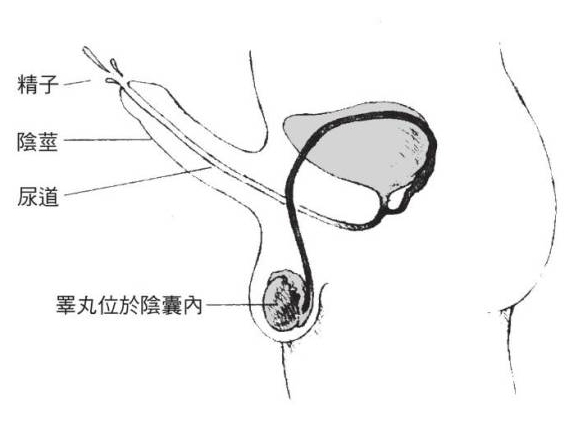
\includegraphics[width=0.7\linewidth]{5}
	\caption{}
\end{figure}

一般情况下,一位男性每次排出的精液为2 -- 6C.C,每C.C含成活的精子为6千万 -- 1.5亿个左右。精液是由精子和精浆组成,精浆又包括前列腺液、精囊液和尿道球腺液等成分,其中前列腺液约占三分之一,精囊液约占三分之二。精浆负责输送精子,并为精子提供能量和营养物质。精浆中主要成分是水,此外还有糖类、电解质、酶类、维生素等物质,这些营养物质是保证精子生存与活动的物质基础。各种液体射出的先后顺序为:首先射出的是约0.1 -- 0.2C.C的尿道球腺液,接着射出的是总量约0.5C.C的前列腺液和精子,最后射出的是约2.0 -- 2.5C.C的精囊液。

\section{男性怎样判断自己的性功能}

性功能是人类的基本本能之一,在生活中的地位是不容忽视的。健康、完善的性功能,不仅是身体健康的标志,而且还影响着人的精神状态、生活品质、生育后代的能力,以及人格魅力等方面,同时也是性文化中不可缺少的一部分。

怎样判断自己的性功能、如何对待自己的性功能,如果缺乏必要的知识积累,难免会走入误区。比如,有的人一旦发现自己的性能力出现一些变化就忧心忡忡,陷入焦虑和困惑,怀疑自己是不是性功能减退了,终日疑神疑鬼,乱吃补药,或者偷偷地去找江湖庸医,结果问题不但没有解决,还引发了别的麻烦。事实上,相当一部分怀疑自己性功能有问题而前去就医的“患者”,在经过相关的医学检查后,并没有发现有什么疾病,所谓的性功能减退,实际是过度紧张造成的。

还有一些人与上述这些人不同,他们一旦发现自己的性功能有问题,“死要面子活受罪”,迟迟不肯看医生,长期生活在巨大的精神压力下,当情况发展到非常严重的地步、不得不就医时,往往病情已经很严重,治疗起来自然相当困难。

怎样正确评价自己的性功能呢?以下几点供参考:

(1)关注性器官的勃起状态

年轻且身体健康、精力旺盛的人无论何时,一旦有性方面的刺激,都会对性产生兴趣,阴茎能迅速勃起;年纪稍长一些的中年人,可能会在勃起之前需要一段时间,这些都是正常的。但如果你发现自己的性器官有时候勃起,有时候不能勃起,或者虽能勃起,但坚持不了多长时间,未到射精时就疲软下来,这种情况常常提示你的性功能可能有所降低,但问题不大,可以通过适当的食补、正确的药补,及科学的锻炼进行纠正。比较严重的情况,是在较长的一段时间里,阴茎始终没有勃起过,这就需要看医生了,应该到医生那里接受检查后,再采取相应的措施。

(2)判断自己性欲产生的方式

怎样判断自己的性功能、如何对待自己的性功能,如果缺乏必要的知识积累,难免会走入误区。比如,有的人一旦发现自己的性能力出现一些变化就憂心忡忡,陷入焦虑和困惑,怀疑自己是不是性功能减退了,终日疑神疑鬼,乱吃补药,或者偷偷地去找江湖庸医,结果问题不但没有解决,还引发了别的麻烦。事实上,相当一部分怀疑自己性功能有问题而前去就医的“患者”,在经过相关的医学检查后,并没有发现有什么疾病,所谓的性功能减退,实际是过度紧张造成的。

还有一些人与上述这些人不同,他们一旦发现自己的性功能有问题,“死要面子活受罪”,迟迟不肯看医生,长期生活在巨大的精神压力下,当情况发展到非常严重的地步、不得不就医时,往往病情已经很严重,治疗起来自然相当困难。

性欲比较旺盛的人,一般都会在性生活中处于主动地位。在有些两性关系中,如果男女双方的性欲强度差不多,常常是男女互为主动,当然也不排除女方主动的情况。如果女方主动,男方能够积极回应,就大可不必为自己的性功能担心。如果你在性生活中表现得很消极,必须依赖对方的主动,或者即使对方主动诱导,也很难激起你对性的兴趣来,说明你的性能力出现了问题。

性能力出现问题,不要消极迥避,积极的应对措施是寻求专业医生的帮助。除了男科医生外,咨询心理医生也是十分必要的。如果没有器质性疾病,措施得当,问题并不难解决。只是一定要科学就医,而不是消极回避或“有病乱投医”。

3)对性的关心程度是性功能的一种表现

性功能包括性生理和性心理两方面的内容。一般情况下,性心理和性生理正常的男性,无论年龄多大,一旦看见性感、年轻、漂亮的女子,都会情有所动,看见妻子裸露的肌肤,“肤色如凝脂”,就会有想抚摸的冲动,这是正常的性反应,不能一概归结为“下流”。如果遇到和自己关系很亲近、很鍾情的女性,只能产生一般的交谈所带来的快乐,而不产生任何性的想像,说明你的性感受开始变得迟钝了,需要想办法去提高自己的性兴奋程度,像治疗軀体的其他疾病那样,寻找病因,进行对症治疗。

\section{适时变换性交姿势}

经过磨合之后,夫妻性生活时的姿势往往就固定下来了,久而久之,可能一如当初时那样美满,但也可能由于一成不变的固定模式,导致性生活品质下降。正确的做法是偶有变化,虽然并不一定尝试每种姿势。

性交姿势又叫性交体位,对性反应的性质和强度,都有很大的影响,如果性交体位不适宜,就会造成性兴奋程度的下降。没有哪一种体位适合于所有的配偶,因此要对其进行探討。夫妇双方的性器官未必十分吻合、贴切,有大、小方面的不适应,要根据这种不适应用不同的体位来补救,并找出最容易达到性高潮的体位。由于性交体位的改变,有助于提高性生活的品质,所以夫妻双方要密切配合,找出更理想、更适合于自己身体条件,和更有利于性感满足的新姿势来,比如可以在一次性交过程中,由一种体位变换到另一种体位,甚至变换好几种体位。常用的性交体位有如下几种:

(1)男上女下(女仰臥、男俯)

这是最传统、最常用的性交体位。随着历史和性文化的发展,人们的人文理念、文化修养、社会习俗,都早已发生了深刻的变化,“男上女下”已不是唯一“正统”的性交体位,人们勇敢地进行着新的尝试,但“男上女下”的体位,仍然被许多人所崇尚和实践着。

“男上女下”的体位,自有其被推崇的理由,但仍有些女性感到男上式限制了她们的活动,另外一些女性则认为这一体位比较舒服,女子正面的乳房、阴阜承受压力,能产生出触觉快感。

(2)女上男下

这种体位能更好地发挥女方在性生活中的主观能动性,因为它在很大程度上,可以由女方自己来控制性活动的进程,比较适合性感超常的女性。此外,喜欢追求刺激性的女性,采用“女上男下”式更易于获得性满足。“女上男下”式能使女方子宫下降,阴道口变宽,所以,即使是阴茎短小的男性,也能给女性比较强烈的刺激,使双方都得到愉悦。

但“女上男下”的体位,不利于对阴蒂的直接刺激,如果女性的会阴口太靠后,或者女性比较肥胖、身体过于龐大笨重,或者女性缺乏经验时,这种体位也会有一些不足。

(3)侧位

将面对面式稍加以修改即为侧位,即女方侧臥,男方面向女方在其两腿之间躺下。这种体位既简单又易于掌握,也十分舒适,因为双方的身体重量基本都压在床上,彼此负重很少,便于保存体力,不会感到劳累。由于这种体位使双方的骨盆向各个方向的活动,都不大容易受到限制,特别是女性可以自由活动,便于掌握节奏,同时还有利于男方对射精的控制,以及用手来刺激女方乳房、阴阜及阴蒂等部位,所以适宜在妊娠期使用,它可以避免对胎儿的压迫,是比较可靠的方法。

(4)后进入式

是男性面向女性背部的一种体位。这种体位可以十分方便地用手对阴蒂进行直接刺激,这样就造成了对阴道区域的更紧密的触动,和施加更大的压力,尤其适合男女双方都很胖的情况。这种体位也适用于妊娠期。缺点是插入不完全,常会使双方都感到生理上的紧张,不像面对面时,双方能够亲密无间地进行拥抱和彼此爱抚。另外,由于阴道入口是由下而上,与阴茎方向相反,可能会给插入带来一定的难度,但一旦插入,其对阴道的刺激也是很强烈的。

\section{和谐的性生活在于高潮的“同步”}

在性生活中夫妻“同步”达到性高潮,是所有夫妻都嚮往和渴望的。然而现实生活中有不少结婚多年的夫妻,都没能达到性和谐的程度,如果这个问题处理不好,可能会影响夫妻感情。

和谐的性生活,不仅可以满足双方的性欲望,还有利于夫妻的身体健康。所以·夫妻应该爭取享受这种性生活最高境界的“同步”。但是,影响性爱达到理想境界的因素十分繁多,可能有相当部分的夫妻,终生刻意探索也没能如愿,可能是他们太过紧张、執着,限制了对性生活的细致体验和充分发挥。

要想达到性生活的和谐,首先要嘹解男女在生理上的差别。男人性欲强·冲动出现快,消退也快,性欲主要集中在生殖器官上,发生性冲动进入兴奋期即急于性交;女人性冲动出现较慢,性欲兴
趣广泛,需要丈夫的爱抚亲吻,性憋产生、增强是达到性和谐的前提。

性爱是两个人之间的事,应该如何进行性和谐的探索,是很个性化的问题。彼此之间的感觉舒服是最重要的,至于要如何做则没有一定的规则可循,只要两人都能好好享受即可。

下面的一些建议,或许可以起到松弛紧张神经的作用,使男女双方获得意想不到的满足感。

①性生活前要做好充分的准备,男人可以采取各种方法来激起妻子的性欲,只有在妻子真正进入了性兴奋状态,性生活才容易获得满意。

②丈夫切忌性急和粗鲁,绝不可只顾满足自己而不顾妻子的意愿。男人要学会控制自己达到高潮射精的时间,可以通过放慢节奏来实现,因为性不和谐,往往来自于女性的高潮出现较晚,女方也不要勉强应付。

③尽量放松,慢慢地体会性过程所带来的感受和体验,而不要把自己的注意力,完全集中在追求性和谐上。

④在性生活过程中,把握自己的每一个举动,让你逐渐地接近理想境界。

⑤男方把自己的感受告诉妻子,得到妻子的理解、支持和有力的帮助,双方互相尊重、互相体贴、配合默契才可以达到性和谐。

⑥男性射精后不要立即结束性器官的接触,还要撑持、与妻子交谈,待妻子达到高潮并性欲完全消失,共同结束性生活。夫妻双方都得到了满足,这样才能使性生活和谐起来。

\section{实现夫妻性和谐的必备条件有哪些}

美好和谐的性生活,需要靠夫妇双方共同努力来实现。为了达到这样的目的,男女双方必须要熟悉自己的和对方的性特点,并具备下面这些条件:

①双方的心理状态良好。夫妻要恩爱,在感情上水乳交融,能创造和谐的性生活气氛;宜选择环境安静、心情欢快的时候进行性生活。双方在性生活中应主动、默契地配合,密切协作,共同充当“二重奏”的主角。恩爱的夫妻关系是性生活和谐的关鍵。

②双方的生理状态良好。性生活前应进行局部的清洁卫生,清除局部不适因素,增加局部润滑感,这是性生活和谐的必要条件。

③双方体魄强健,精力充沛。双方生殖器发育正常,是保证性器官接触、获得正常性刺激的生理基础。选择身体健康的时候进行性生活,能两情欢愉,如魚得水。

④掌握科学的性知识。正确掌握性生活的四个性反应周期,根据男方性冲动较快、女方性冲动较慢的特点,男方多刺激女方动情并要耐心等待,等到女方有性兴奋后再开始交接,可使双方的“性欲高潮曲线”趨于重叠,达到男女双方性生理上趨于同步。

夫妻间性不和谐的主要原因是性知识的缺乏,例如缺乏必要的性知识、不会性交、不会摩擦抽动阴茎、不知道对方的性反应特点、不关心对方的性反应等,因此双方无法完美配合,性生活也就难以达到和谐的境界。

性和谐以及对性和谐的要求,在不同的夫妻之间是有着明显差异的。要想获得和谐的性生活,只有夫妇双方的积极性同时调动起来,共同实践、探討、交流,才能共同达到性爱的完美境界。

\section{爱侣间永保性爱和谐美满的秘诀是什么}

美满和谐的性生活,有赖于爱侣双方情感的交融,将性爱与情爱融为一体,包括以下几个方面的内容:

①婚前注意彼此检点。许多婚后的性与情感的不和谐,都与婚前的性行为或性经验有关,是导致夫妻生活不和谐的禍根。

②婚后避免缺乏新意和激情的性交。切忌“千篇一律”的性生活,不要为了性而做爱,而应该为了爱而做爱。共同创造新生活,不断地变换做爱的环境、地点、姿势和体位,这样做才可能不断地密切夫妻间的关系,使婚姻能经受住风雨的考验。

③要体谅对方。在对方不能满足你的生理要求时,不要太过计较,过多的责备是要伤感情的,而过分的强求生理满足,可能使对方厌倦性交,甚至出现各种各样的性功能障碍或性冷淡。

④能够达到肉体与精神的和谐美满。这当然是爱的重要表达方式,但绝对不是唯一的方式,爱的表达形式体现在生活中的点点滴滴。所以,平时要经常表达自己对配偶的爱意,充分体现自己的魅力,为爱创造温馨的气氛,而不是只在做爱的时候才进行情感的沟通。

\section{真爱不需要太多的技巧和艺术}

情爱与性爱是密不可分的,情爱可以啟动性爱,而性爱又可以反过来强化情爱,无论单纯地强调哪一种爱,都有失偏頗。在现实生活中,有些人往往过分地强调了性爱,尤其是性交的技巧和艺术性,强调了性交动作、姿势和花样上的翻新,强调了性爱的创造性,强调了性爱的品味、品质、档次和环境,这样做真的有必要吗?

由于传统文化的影响,多数人都持有这样一种观念,即性生活是否美满取决于男方,尤其是男方在性生活中的技巧如何,因此把注意力全部集中在有性感受器官的身体部位上。其实,性反应涉及眾多的生理和心理反应,尽管其中的一种或几种可能起着重要的作用,例如性交过程中全身肌肉的紧张度,但其他的反应也是不可或缺的,例如强烈的情爱表达和流露。

我们承认,科学地掌握性技巧是个前提。

①要双方绝对自愿并真正需要,否则将是侵犯对方的人格尊严,而且会造成双方的心理伤害,也不会产生好的效果。

②夫妻感情良好。

③双方性知识和性态度的水准非常接近,彼此容易沟通和接受对方的安排。

④所用的性技巧必须是具有科学性的,并要准确掌握其适用范围,这样性生活才会产生有益的效果。但性技巧本身既不能制造爱情,也难以充分地沟通夫妻间的感情。如果过分强调性技巧,会对感情产生不良作用,使性爱的行为变成一种机械的动作,极易导致双方或一方产生疏远、孤独、人格受侮辱等不良情绪,削弱了性爱与情爱之间的必然联系。

真爱不需要太多的技巧,让性欲顺其自然地发泄就是最好的,如果人工“制造”性爱的味道浓了,性爱的负担也就产生或增加了,紧张焦虑情绪也就出现了;而随心所欲、顺其自然的自然发挥也就少了。

正处在精力充沛、激情亢奋阶段的青壮年男人,完全可以要风得风、要雨得雨,没有必要寻找所谓的性爱的感觉和性爱的技巧,随意发挥都是真情的流露和刻骨銘心的记憶;处在激情不再阶段的中老年男人,也应该是坦坦然然,平平淡淡才是真,跟着感觉走的感觉最好,而不需要刻意强求。实际上,最高級、最通用的“性技巧”不是动作上的而是心灵上的,是尽可能多地把爱慕、依恋、亲密和关心之类的真情倾注和浓缩于性生活之中。

所以,迷信性技巧而又忽视情感交流的人,其实是在自討苦吃。做爱不要太苛求自己,不要太講究技巧和艺术,只要自我感觉不错、跟着感觉走就行了。

\section{不宜过性生活的几种情形}


性生活是已婚男女天经地义的快乐享受,性生活的快乐程度,取决于夫妻双方是否全身心投入和彼此是否倾心配合。此外,不适当的环境、情绪、身体健康状况等因素,都可能限制人们随心所欲地进行性生活。一旦出现以下几种情形,应该避免性生活:

①生病。尽管疾病并不是性生活的对禁忌,但是在患有某些严重疾病,或者疾病的急性期内,一般是要禁止性生活的。因为性生活会对患者自身的健康和疾病的恢复,构成一定的威脅。慢性疾病或者疾病的恢复期内是否能够过性生活,需要获得医生的指导意见。患有性病的夫妻,一定要在性病治愈之后,并渡过了传染期,才可以过性生活,否则勉强过性生活,受害者不仅是自己,还会通过性器官的接触,而将疾病传染给对方。

②过度疲劳。性生活是要消耗很大体力的,且身体或精神疲惫时过性生活,往往不容易达到高潮,收不到双方满意的效果。劳累后立即过性生活,还会损害健康,并容易诱发早泄、遗精、阳痿等性功能障碍。

③心情不佳或心绪不宁。有些夫妻在一方情绪不佳或心绪不宁时勉强过性生活,不但得不到性生活的美满和谐,还会使情绪不好的一方对此产生反感,引起夫妻感情不和;如反覆发生类似情况,还会导致女子的性冷淡或男子的阳痿或其他疾病,例如夫妻因为生活琐事吵嘴后、夫妻问由于担心怀孕而顾虑重重等。

④酒后。一些人习惯酒后行房事,有人甚至认为酒后过性生活会“提高品质”,能延长性交时间,尤其是一些早泄患者。其实,酒后,尤其是大量饮用烈性酒后,性生活会造成许多危害,例如射精疼痛、血精等,还可以导致性功能多种障碍,最终会妨碍性生活和谐,而且如酒后受孕,还会给胎儿带来负面影响。

⑤不講卫生。性器官的卫生状况,直接关系到夫妻双方的身体健康。生殖器官的不清洁,可以将细菌等病原体带入对方体内,构成了对健康的威脅;反之,清新、整洁的卫生状况,不但有益于夫妻双方的健康,还可以增强性感受,有助于性生活的和谐和美满。

⑥准备不充分。性生活前的准备,是夫妻间心理和生理进入“状态”的必要阶段,不可或缺。如果倉促进行性生活,并草率收兵,不仅难以让妻子达到性高潮,甚至会给她带来痛苦,久而久之会使她对性生活丧失兴趣,是产生性冷淡的主要原因。

⑦饱食或饑饿时。饱食可以使胃肠道充盈,大脑及全身各个器官(包括性器官)相对地血液供应不足,影响阴茎的勃起程度,故不宜在刚刚吃完饭后就过性生活;饑饿时人的体力下降,精力不充沛,此时过性生活也往往达不到满意的效果。

⑧精神过度紧张、抑郁、焦虑。精神极度紧张、抑郁和焦虑,易引起男性的早泄和阳痿,或女方的性交疼痛(阴道痉挛)。所以,夫妻性生活时,要尽量保持轻松、愉快的心情,这样才能保证性生活的品质。

\section{什么是性激素}

男性的睾丸和女性的卵巢都是性腺,其分泌出的与人体性器官发育和性功能等有密切关系的类固醇样的物质,即性激素。男性性激素主要是雄性激素,即睾酮;女性性激素主要是雌激素和孕激素。它们直接进入血液发挥不同的生理作用。

性激素的主要作用有:

①促进性器官发育并维持其成熟状态。雄激素可促进男性性器官发育、成熟,并维持其成熟状态;雌激素可刺激和促进女性子宫、输卵管、阴道、外阴等器官的发育、成熟,并维持其成熟状态。另外,卵巢产生的孕激素与雌激素,能协同完成调节女性的月经周期和生育过程。

②促进第二性征的出现。睾酮具有刺激男性鬍鬚生长的作用,因此,男性会长鬍鬚。睾酮能促进蛋白质合成,使人肌肉发达。雌激素能促进女性皮下脂肪沉积,使其皮下脂肪丰富。雌激素可促进乳房的腺管增生,孕激素可促使乳房的腺泡发育,因此,女性的乳房会发育得较大。睾酮还有促使男性喉结增大、声带增厚的作用,所以男性发音会显得低沉。正因为男女性腺不同,睾丸和卵巢产生的内分泌激素不同,因而各自会出现不同的性特征。

③维持性功能。性激素能引起性中枢兴奋。男性缺少睾酮或女性缺少雌激素,均可引起性欲减退或性功能障碍等。男性严重缺乏睾酮,可使精液量减少,而雌性激素的分泌,可使女性在排卵期前后表现出较高的性反应性。所以,性激素是维持男女性功能的物质基础。

④促进人体的新陈代谢。雄性激素最重要的作用是促使蛋白质合成,如使骨骼生长、体重增加、体格健壮;促进骨髓的造血功能,使红细胞与血红蛋白增多,并减少体内贮存的脂肪。雌性激素能改变体内脂肪的分布,使皮下脂肪含量增加;同时对糖代谢和蛋白质代谢也有一定影响,并能促使骨骼鈣质沉着及骨骺闭合等。孕激素可使身体内基础代谢增强,体温稍有升高。

\section{什么样的精液才正常}

精液有正常和异常之分。什么样的精液是正常精液,根据世界卫生组织的规定,可以从以下几个方面进行判断。

①精液量。正常的精液量≥2C.C。大于6C.C时为过多,不但精子密度降低,而且易从阴道中流出,常见于精囊炎;小于2C.C为精液量过少,但通常以1C.C以下为过少,此时的精液与女性生殖道接触面积小,或因黏稠,不利于精子进入女方宫颈口而易导致性交困难、不育,常见于严重的附属性腺炎症、睾酮水准低下、射精管梗阻、逆行射精等。

②颜色。精液的正常颜色是灰白色、乳白色或略带黄色。乳白色或黄绿色,提示生殖道或附属性腺存在炎症;粉色、红色,显微镜下见红细胞者为血性精液,常见于附属性腺、后尿道的炎症,偶见于结核或肿瘤。

③酸碱度。精液正常的pH 值为≥7.2。小于7.2见于射精管梗阻或受尿液污染;pH值过高者,见于精囊炎症或标本陈旧。

④液化时间。正常精液射出后为胶凍状,5~30分钟后变为液体。如果精液射出30分钟后仍不液化,属于液化延迟,60分钟后仍不液化属于异常,即“精液不液化”。

⑤黏稠度。将玻璃棒接触已经液化的精液,轻轻提拉,可形成精液丝,正常时其长度小于2公分。

⑥精子数。一般以每C.C精液中的精子数表示,正常计数的精子密度≥20X10/C.C。精子密度小于20X10/C.C为精子密度过少,精子总数少于40X10°为少精子症,见于各种原因导致的生精功能障碍等,可因精子进入子宫腔及输卵管的机会减少,而致生育力低下或不育。如精子密度大于250X10/C.C为精子过多,因其活动力及功能状态不佳,也可导致不育。

⑦精子形态。正常形态(健康)的精子应≥4\%,畸形精子症可显着降低生育潜能,甚至可造成不育。

⑧活动力。精子中呈直线向前运动者≥50\%。

⑨存活率。射精后1小时内精液中的活精子≥50\%。导致精子活动力及存活率降低的常见原因,有附属性腺炎症、精索静脉曲张、慢性呼吸道感染引起的纤毛呆滯综合症、精液中存在抗精子抗体。白细胞数量。正常精液中白细胞<1X10°/C.C。白细胞增多表明生殖道或附属性腺存在炎症或感染。

\section{阴茎的大小会影响性生活品质吗}

一般来说,阴茎大小并不代表其性功能的强弱,也不能作为评价性能力的标准。疲软状态下男性阴茎长度大于4公分即可行使正常性功能。如果阴茎在青春期后短于4公分,而且没有勃起功能,特别是第二性征发育不良,无精子且无生育能力,才可被认为是阴茎发育不正常。男性阴茎无论大小,只要勃起功能良好,能顺利插入女方阴道,并能在阴道内反覆抽动射精,同时配合适当的性交技巧,女性所感受到的性刺激基本是相似的。当积累了一定的性交经验,并掌握了各种性交姿势与技巧之后,绝大多数的夫妻在性生活方面都会感到满意。即使阴茎比较短小,只要发育正常,勃起功能良好,也不会影响性生活的美满与和谐。因为在勃起状态下,阴茎大小的差距不是很明显。

阴茎大小存在着明显的年龄差异。儿童期男性的阴茎较小,到了青春期阴茎开始长大,且颜色加深,成年后相对穩定,但其长短不一、粗细不等属正常生理现象。阴茎大小有一定範围,但多大才算正常,这并没有一定的医学标准,一般通过測量阴茎长度(自阴茎根部到尿道外口)和阴茎周径来衡量。泌尿外科专家曾对一百例进行婚前体检的正常男性青年做了常态下阴茎測量,其測量结果发现,阴茎长度在6~9公分的人共93人。一家医院泌尿科测量结果证实,一般青年男性的阴茎平均长度为6.55公分(未勃起状态下)。一般认为,我国男性的阴茎长度多在6~9公分之间,阴茎周径多在7~9公分之间。但这并不是評定阴茎大小是否正常的标准,也不能说明不在此範围内的阴茎就一定不正常。一般情况下,阴茎的大小对性生活不会产生实质性的影响,除非过大或过小。

阴茎大小存在个体差异,能够影响阴茎大小的因素有很多种,包括身体脂肪过多、天气过冷、压力等,但与身高没有直接关关。性医学专家认为,阴茎大小主要与种族和遗传有关。一般认为同等身高,白种人与黑人的阴茎要大于黄种人。阴茎大小也受遗传因素的影响。

\section{介紹 9 种可以增强性功能的食品}

吃出健康在现实生活中的意义越来越大,食物撩法已被广泛应用于疾病的治疗和预防保健,很多食物能增强男性的性功能,在这里简单介紹一下。

①韭菜,又叫起阳草、懶人菜、长生非、扁菜等,不仅质嫩味鮮,营养也很丰富,除含有蛋白质、脂肪、碳水化合物、鈣、磷、鐵、维生素C、胡蘿蔔素外,还含有较多的膳食纤维,能增加胃肠蠕动,对习惯性便秘有益,对预防肠癌有重要意义。韭菜含有挥发油及含硫化合物,能促进食欲、杀菌和降低血脂。韭菜还是一味传统的中药,其温补肝腎、助阳固精作用突出,所以在药典上有“起阳草”之名。韭菜子为激性剂,有固精、助阳、补腎、治带、暖腰膝等作用,适用于阳痿、遣精、多尿等疾病患者。将韭菜子研粉,每天早晚各服15公克,开水送服,对治疗阳痿有效。

②淡菜含丰富的蛋白质、碘、B群维生素、鋅、鐵、鈣、磷等。其味鹹,性温,有温腎固精、益气补虚功效,适用于男性性功能障碍、遗精、阳痿、疲劳、消渴等症。男性常食可强壮身体,增强性功能。

③中医认为荔枝味甘,性温,有补益气血、添精生髓、生津和胃、丰肌澤肤等功效,既可健身益颜,又可用于治疗病后津液不足及腎虧梦遣、脾虚泄潟、健忘失眠。常食荔枝能改善人的性功能,对遗精、阳痿、早泄、阴冷诸症有辅助治疗作用。阳痿早泄者,取荔枝干10个,五味子10公克,金樱子15公克,用水煎服,可强身健体。

④中医认为枸杞子味甘,性平,入肝、腎、肺经,有滋补肝腎、益精明目、和血润燥、澤肤悦颜,培元烏发等功效,是提高男女性功能的健康良药,可用于治疗肝腎阴虛、头暈目眩、视物昏花、遗精阳痿、面色暗黄、鬚发枯黄、腰膝酸软、阴虛劳嗽、老人消渴等症。枸杞子有增强机体免疫功能、促进细胞代谢、降低血中胆固醇含量、抗动脉粥样硬化、改善皮肤弹性等作用。常服枸杞子,可延缓衰老、美肤益颜及提高性功能。枸杞子有兴奋性神经作用,性欲亢进者不宜食用。

⑤松子是重要的壮阳食品。中医认为松子仁味甘,性微温,有强阳补骨、和血美肤、润肺止咳、滑肠通便等功效。松子仁中含有较多不饱和脂肪酸、优质蛋白质、多种维生素和礦物质。经常食用有强身健体,提高机体免疫功能、延缓衰老、消除皮肤皱紋、润肤美容、增强性功能等作用,对食欲不振、易疲劳、遗精、盗汗、多梦、体虚、缺乏勃起力度者有较好撩效。

⑥蝦味道鮮美,补益和药用作用都较高。传统医学认为,蝦味甘、鹹,性温,有壮阳益腎、补精、通乳之功。凡久病体虚、气短乏力、不思饮食者,都可将其作为滋补食品。人常食蝦,有强身健体的效果。

⑦牡蠣又称蠣蛤、蠔子,含有丰富的鋅元素及鐵、磷、鈣、优质蛋白质、糖类及多种维生素。其味鹹,性微寒,有滋阴潜阳、补腎涩精功效。男性常食牡蠣可提高性功能及精子的品质,对遗精、虛劳乏损、腎虛阳痿等有较好的食疗效果。

⑧泥鳅含有蛋白质、脂肪、维生素A、维生素B1、煙酸、鐵、磷、鈣等营养物质。其味甘,性平,有补中益气、养腎生精功效,对调节性功能有较好的作用。泥鳅中含一种特殊蛋白质,有促进精子形成作用。成年男性常食泥鳅可滋补强身。

⑨羊腎又叫羊腰子,含有丰富的蛋白质、脂肪、杂生素A、维生素E、杂生素C、鈣、鐵、磷等营养物质。其味甘,性温,有生精益血、壮阳补腎功效。适用于腎虚阳痿者食用。

\section{爱抚阴蒂的技巧}

爱抚阴蒂,是多数人在性爱的过程中不可或缺的“性趣”技巧,如果掌握好时间和程度,运用得当,可以让女性获得更为充分的满足。

(1)必须适时和适度

有些女性必须要经过爱抚阴蒂才能达到性高潮。阴蒂附近是相当敏感的地带,要充分地利用十指,慎重地加以爱抚,不能太过生硬和草率。最好的方式是先用手指去按摩耻骨上方附近,待阴蒂的敏感度增高后,再去慢慢接近阴蒂。

爱抚阴蒂成功,会产生很大的快感,甚至能促使女性达到高潮。

(2)不要忘记爱抚其他性敏感区

能够激起女性性欲的另外一种方式是爱抚脖子、腋下、腕、脚等部位,可以先于对阴蒂的按摩,从上而下,以直线的方式加以刺激,这种方法可以使爱抚阴蒂更为顺利。

(3)按摩背部和大腿

按摩背部和大腿,是为了让女性处于一种十分放松的状态,像画圆画似的搓揉,女性在轻柔的按摩中,抗拒心理会慢慢消除,这也有利于进入爱抚阴蒂的状态。此外,对于臀部、乳房、乳头进行按摩,比如,一边画着小圆,一边从内侧到外侧用4根指腹进行按摩,会有明显的效果。臀部的中央稍上附近是一非常敏感的地带,用食指和中指从肛门方向向腰部压入,下半身的敏感度就会很高。

\section{身体的哪些部位是性的敏感区}

对性的体验存在着明显的个体差异,这与每个人的性敏感区有很大的关系。其实,性的敏感区不仅仅是性器官,它还包括乳房、乳头、口唇、腹部、耳垂、腿内侧、颈背部、腋下、臀部、性器官周围的皮肤以及脚趾等部位,如果能在性生活中对这些部位进行轻柔的按摩或刺激,可以降低性紧张度,增加愉悦感。

所以,新婚之夜或初次性体验之后,每个人都会知道自己的性敏感区在哪里,并要告知对方,这样性生活才容易顺利,能避免很多麻烦。

过好性生活是新婚男女的必修課,在这一学习的过程中,可以尝试多个性敏感区。就一般规律而言,按揉乳房是可以激起性欲的,乳头则更敏感,会增加性欲的强度;口唇的皮肤很薄,对异性的刺激反应很快;腹部,尤其是下腹部不容忽视,因为这里可以提高性的反应并促使产生性期待;轻揉耳垂,能快速傅递性快感;臀部对比较强有力的按摩有反应;可能很多人都容易忘记,脚趾趾腹也是性的敏感区,不能小视,它可以引发全身的性反应。

可能,一些人对开发身体的其他性敏感区会心存芥蒂,或羞于啟齿,这是不科学的,在性爱过程中获得更多的愉悦感,既是美的,也是健康的。

\section{什么是G点}

G 点是女性的性敏感区,位于阴道口约三分之二的地方,在性反应中比阴道前端要敏感,但不容易感知它的存在。在性生活中,男性如果能够找到G点并给予适当的刺激,女性是可以获得性快感的。

G 点很敏感,性交中的任何体位都能刺激阴道,但正常体位及背后体位比较容易找到G点。记住,插入不要过深,朝着G点给予刺激,像画圆的动作来进行性运动即可。

\section{怎样调整性生活的频率}

这是一个较难回答的问题,性欲的强弱因人而异,即使是同一个人,也受年龄、体质、性格、職业、气候、环境、情緒等多种因素的影响。因此,性生活的次数不能机械地规定,而要根据双方身体的具体情况做适当调节。

成年后随着年龄的增加,人类的各种生理机能将逐渐减退,性机能也不例外,也将随着年龄的增加而逐渐下降。有人分析了相关的资料后发现,30~34岁的男人,每周的平均性生活次数是2.2次,以后逐年减少,到60~64岁时的每周性生活次数平均仅0.7次。所以,根据年龄的变化,一般推荐性生活的频度为:

①新婚阶段:每周3~5次或更多。

②青壮年期:每周2~3次。

③40~50 岁:每周1~2次。

④50~60岁:每月2~3次。

⑤60~70岁:每月1~2次。

⑥70~80岁:每1~2月1次。

⑦80岁以上,每1~4个月1次。

夫妻久别重逢,往往性交较频,这是人之常情,但也要适当节制。

频度合适的性生活,会给生活带来巨大的愉悦,而过于频繁的性生活,可能会给健康带来不利的影响。你的性生活频度是否合适,可以根据性生活后的感觉来判断,以不出现明显的疲劳、精神委靡、腰膝酸软和全身乏力为度。如果出现无精打采、头暈腰酸、心跳气短或食欲不振等,则说明性生活过度,就应当有所节制,适当延长性生活的间隔时间。有少数性欲旺盛的夫妇,向来性交频繁,而双方仍心神爽快、精力充沛,也应该认为是适当的。

有些人容易放纵自己,沉湎于频繁的性生活不能自拔;有些人将性交次数,看做是显示男人力量和尊严的象征;也有的人只是为了单方面地迎合和全力满足妻子的性要求。因此,这些人极其容易过分强化自己的性意识,企图在最短的时间内再度勃起,用意志的力量,支撑疲惫不堪的身体进行性生活,这对身心健康会有很大的危害,是不值得提倡的。盲目地推崇高数量性生活的结果,是无形中加重身体和心理负担,一旦年龄较大,或偶然遇到特殊情况而不能保持高频率性交,就会怀疑自己患了性功能障碍,甚至会对自己的整个人格和人生目标产生怀疑或失望。男性的性生活实践也并非“多多益善”,多数的丈夫在亲身的性生活体验中,会渐渐地发现自己的性需求,实际上在悄悄地变化,从需要大数量转为寻求高品质,希望获得更深切的情感交流和体验。

\section{怎样延长性交时间}

性交时间没有绝对的标准,一般为2~6分钟。在性交的过程中,男方坚持的时间越长,女方达到高潮的可能性就越大,如果时间太短,女方不易达到性高潮。

如何延迟射精而延畏性交时间,可以通过以下几种方法来达到目的。

①精力不要过于集中。如果做爱时全身心地投入,意念就会集中在阴茎头上,甚至有自己全部身体融进去的感觉,如果此时分散一下注意力,会缓解射精的冲动。

②机械压迫阴茎头。这也可延迟射精冲动。

③ 戴避孕套。使用避孕套后做爱时间一般会比较长。此外建议男性增强体质,一般体质较好的男人做爱时间要长些。除锻炼身体外,还要注意营养。男性和女性之间需要默契的配合,做爱是两个人的艺术,女性善于引导,男性可适当延长性交时间,而女性可获得足够的性满足。男性在即将达到高潮前改变性交姿势,能适当控制住射精欲望,这也能延长性交时间。

\section{抽煙、酗酒影响性功能}

性功能的健康与否,受许多因素的影响,其中不良的生活方式会有相当大的影响,特别是抽煙、酗酒等。据统计,吸煙者中正常精子数会减少百分之十左右。若每天抽煙20~30支,精子畸变率显着增高。吸煙时间越长,畸形精子越多,精子活动力也越低。研究结果还表明,吸煙还可以引起动脉硬化,百分之九十以上的吸煙者阴茎血液循环不良,阴茎勃起速度减慢,阳痿患者中有三分之二是吸煙者。

酗酒会对生殖系统产生更为严重的不良影响。酗酒可加速体内睾酮的分解,造成雌激素水准相对增高,睾丸萎缩,导致阳痿;过量摄入酒精,会引起胚胎发育异常、流产、低能儿,国外称这种低能儿为“星期天嬰儿”,是父亲酗酒的结果,所以酗酒不利于优生。

尤为值得一提的是吸毒对性功能更不利,大麻、海洛因和美沙酮等,会使血液中睾酮水准降低而影响性功能。有资料报导,海洛因嗜好者中,性欲抑制者占百分之百;美沙酮嗜好者,性欲抑制百分之九十六。两者均可导致性功能障碍。此外,不要无故长期濫用药物,如治撩高血压药物氯噻嗪类利尿剂、安体舒通、利血平、心得安,镇静剂安定、利眠宁、安眠酮等,对性功能均有抑制作用。

\chapter{叫床}

在性生活时“叫床”者多数是女性,这主要与神经反射有关。

在性活动中,女性本能地接受刺激,并有强烈的表达欲望,于是就会发出“叫床”的声音。

“叫床”可以说是正常现象。“叫床”的情形有三种。

第一是在性高潮中无意识地、反射性地发出声音。

第二,通过“叫床”增强性反应,有些女性会因为听到自己的声音,而产生无比强烈的性兴奋,“叫床”的目的是为了尽快达到高潮。

第三,通过“叫床”宣泄性感受,或者提示对方,想结束性生活。

\section{心理疲劳影响性生活品质}

性问题常常令人难以啟齿,解决不好,会导致性功能障碍。进入婚姻状态以后,在琐碎的日常生活中,夫妻间的感情归于平淡,再加上患病和衰老,心理疲劳就会接踵而来。但在现实生活中,的确有一部分人是既健康又没有衰老,只是长期抑制自己的性欲望,其原因也是日积月累的心理疲劳。

心理疲劳是一种不健康的状态。导致心理疲劳的常见原因,主要是来自生活、工作、婚姻、健康及其他方面的受挫感。人的内心需要精神力量的支撑,自信心遭到打击之后,容易委靡不振、唉声歎气、怨天尤人。如果单纯地从生理医学的角度看,产生性欲是人的一种本能,它会在人体衰老之后逐渐减弱,并受心理因素的影响。如果能在工作、生活中建立起充分的自信心,调整好状态,生理上的性欲就能顺利地表现出来。遭遇挫折后的紧张、焦虑、怨恨、抑郁等不良情绪,都是扼杀性欲的杀手。

受挫之后重建自信并不困难,只要有正确的价值观,勤于学习和积累,在各种环境中勇于锻炼,自信就会成为陪伴你终生的心理能力。这样一来性的心理疲劳就会远离你,不会侵袭到正常的性生活。

\section{禁欲对性功能有影响}

人类大脑是掌握情欲的关鍵,当欲念在脑海里出现时,刺激会
经由脑丘下部转移到脑下垂体,让人体产生想要付诸于“性”的冲
动,进而对阴茎发出“勃起”的指令。男性阴茎的海绵体,富含平
滑肌及血管内皮细胞,如果长时间没有勃起充血,这些平滑肌就会
逐渐退化,从而影响到海绵体的充血功能。若是长期刻意地压抑欲
望,人体会对以上的刺激模式产生陌生与疏离感,久而久之,在阴
茎缺乏锻炼的情况下,运动神经也会变得迟钝,甚至退化。正常的
男性若是长时间禁欲,首先会对心理层面产生负面影响,进而引发
性功能障碍。自发性的性欲是一种自然的生理反应,所以不要过度
压抑它。已婚男女或是有固定性伴侣者,性欲有正常宣泄的管道;
若是单身或是配偶长期无法进行性生活者,建议在性欲高涨难耐时
进行适度的自慰。

\section{饮酒后不宜性交}

饮酒对性生活是不利的。大量饮酒后,人很快会由兴奋期转入
抑制状态,如果此时有性生活容易出现问题,最常见的问题是阳
痿。即使是少量饮酒,人体处于短暂的兴奋状态,性生活时也易
变得过分激动或粗野鲁莽,还可能发生射精障碍(早泄或射精延
莲)。酒精对人体心脏、肝脏、神经等多种器官具有一定的损害作
用。如果全身状态已不甚良好,再加上性生活时神经系统高度兴
奋,性器官广泛充血,对身体的危害就更大了。

酗酒对生殖系统有很大影响。酗酒可加速体内睾酮的分解,造
成雌激素水准相对增高,使睾丸萎缩,还可能导致阳痿。即使酗酒
后能够成功地完成性交,也不一定是好事。由于酒精可影响精子的
正常发育,造成精子畸形,不利于优生,在这种情况下受孕,会引
起胚胎发育异常、流产、低能儿,将来有可能生下癡呆儿。有调查
发现,那些在星期六或星期天酗酒的男性,当天进行性生活使女性
怀孕生下的孩子,先天畸型的发生率很高,因此,酒后不宜性交,
以免影响男女双方性生活的和谐和后代的健康。

\section{错班夫妻,别错过性爱}

为了謀生或为了追求事业,许多人整日奔波劳碌,错过了太多
的美好生活体验,特别是错班夫妻。由于作息时间的差异,错班夫
妻的亲密生活时间相对减少,有时性爱时间也被压缩或不得不取
消,让许多原本十分恩爱的夫妻,难以尽享生活美事,甚至感情渐
渐流于平淡。调查发现,白班夜班混合的夫妻性生活频率低,并且
品质差。

(1)错班夫妻遭遇生理尴尬
在夫妻性生活中,男女最终会出现高潮,并带来身心的极大愉
悦。如果因“错班”而错过性爱,并且这种不利局面长期不能得到
有效改变,长时间无性生活或倉促性交,就会耠夫妻健康带来不同
程度的伤害。主要表现在:
①体质下降。性生活的良好状态,是有利于增强身体健康的,
性生活过程中的体力消耗和运动,可以起到锻炼全身各个系统功能
的作用,有助于缓和有害的紧张状态,还能帮助消耗热量。
②性欲和性功能降低·经常抑制性生活,将会造成明显的性欲
低下和性功能障碍,这种“发用性”萎缩所造成的性能力的伤害较
为普遍。
③倉促性爱品质低。性生活如过于急切、简单和制式化,忽视
情感需求,将极大地伤害彼此的人格与情感,虽有“性”,却无
爱,带给对方的会是痛苦和厌恶,而不是身心愉悦。

(2)错班夫妻心态难平
保持一定频度的性生活,是夫妻间密切感情、傅遞爱意的重要
手段。如果长期缺乏亲密爱意的明确表达,可能会让彼此产生情感
裂隙,因此而出现抑郁或猜忌的夫妻不在少数。
(3)刻意协调可扭转被动局面
错班夫妻如果能采取适当的措施调整这种状态,就能有效地扭
转现实生活中的被动局面。具体方法主要包括时间的调整和性爱方
式的调整。

①“清晨性爱”。错班夫妻,没必要循规蹈矩,学会利用有限
的时间、注意保证性爱品质非常重要,可以选择彼此重叠时间完成
性交,例如清晨或周末,同时要学会体恤对方,不要奢求性爱次
数。

②边缘性行为。性生活不仅仅意味着性交,短暂的调情或一些
亲密接触的小游戏,例如拥抱、热吻、(包括对性器官的)抚摸、
言语调情等,运用得当,同样可以达到性爱的目的。其实,多数夫
妻最看重的并不是性交的过程,而是感情交流,而边缘性行为是实
现情感交流的有效手段。
③情感鋪垫。给对方以实实在在的关爱,能非常有效地彌补相
处时间上的局限和不足,并真正赢得对方的理解和支持。


\section{老年人太兴奋时别过性生活}

对于中老年人来说,保持和谐美满的性生活非常有必要,但安
全地过好性生活则更加重要。
兴奋是人体的正常反应之一,指人体受到足够强的刺激后产生
的生理现象,此时往往会有神经冲动的快速释放、肌肉的收缩,及

腺体分泌的增加等一系列反应,出现心跳加快、血压升高、头痛等
症状。性生活本身就是一个神经兴奋受刺激的过程,如果在本身已
经很兴奋的情况下去过性生活,中老年人的心跳和血压就会进一步
加快和增高,甚至可以超过身体的耐受限度,轻者出现心慌、头暈
等不适,重者可能会引发心脑血管意外,危及生命安全。现代医学
证明,交感神经的过度兴奋及腎上腺素的刺激,是高血压、冠心
病、心动过速等疾病的重要发病因素。所以,无论平时身体条件怎
么样,为了安全起见,中老年人情绪过于兴奋时最好避免性生活。
情绪兴奋十分常见,如专业人员晉升、论文发表、彩券中獎、
多年的心愿终于实现等,都会使人体处在极度亢奋或过于兴奋的状
态。除了过于兴奋外,情绪激动时也不适宜过性生活,例如家庭慘
变、巨額財产丧失等。情绪激动可使人体血中儿茶酚胺含量增加,
心室颤动的值降低,此时过性生活会增加心脏疾病的发病机率。
中老年人要在性问题上審时度势,遇事努力稳定情绪,性生活
前尽量保持心情平和,尤其是要让心慌、头痛等不适感觉的程度降
低下来,然后才过性生活,并且要迥避劇烈的性交方式。如果经常
出现因兴奋导致性欲亢奋的情况,就需要寻求专科医生的帮助了,
例如检查是否内分泌激素出现了问题。当然了,配偶间应相互帮
助,可通过聊天、出去散步等其他事情来转移注意力,稳定情绪。

\section{“百里不同房,同房不百里”}

经验之谈的“百里不同房,同房不百里”是一句古老俗諺,意
思是在身体状态极度疲劳不堪的情况下,不要进行性交,这是有科
学道理的。所谓的“百里不同房”,是指长途行走以后不宜马上性
交;“同房不百里”指的是性交后不宜马上长途行走。当然,广义
的“百里”还包括劇烈运动或过度劳动等情况。
在长途行走或过度劳累以后,人未经适当休息就进行性生活,
肌肉骨骼和性器官同时需要大量的血液供给,就会造成血液“供不
应求”的局面,一方面使血液难以保证生殖器官的“重点”供应,
容易让局部的充血状态不充分,使得男人的阴茎不够坚挺,女人的
感受不够强烈;另外一方面会使供应肌肉骨骼的血流量大大减少,
从而导致全身酸软无力,难以支付性交所需要的体力;同时,还加
重了心脏的负担,要通过加快心脏跳动的频度,来应付运动器官和
生殖器官对血液的需要,往往会导致出现“顾此失彼”的尴尬境
况。反之亦然,如果在性生活后马上从事劇烈的体力活动,也会让
人体的心脏和血液系统顾此失彼、疲于奔命。偶尔如此,对身体健
康和性和谐的影响不会太大,但如果让类似的情况频繁发生,最终
会影响到中枢神经的调节功能,对夫妻双方的身体健康、性健康和
心理健康都构成最重的威脅。
实际上,“百里不同房,同房不百里”还含有另外一层意思,
即如果在身体过度疲乏的状态下勉强同房,由于上述的不利因素,

必然造成性生活品质不高,而且人体的功能状态,也容易因疲劳而
不能胜任,这不仅对疲劳者的自身健康十分不利,还可以影响到双
方的性感受,夫妻难以在性生活中感受到巨大的身心愉悦,使得
性和谐难以维持“百里”之久,使得双方对性生活的愉悦感受降
低,甚至可以使得过度劳累一方,对性生活产生厌烦和恐惧情绪,
“性”将变得不再重要,甚至可能成为负担,还可以出现诸如阳
痿、早泄、不射精、射精延迟、性快感减低、性冷淡等不同程度的
性功能障碍,这不仅会影响到夫妻问的性和谐,还会影响到夫妻间
的感情,甚至导致感情破裂,使夫妻难以白头偕老地走完“百里”
人生.

工作过于紧张忙碌的上班族,特别是那些要在白天辛勤工作、
经常加班到半夜的人们,必须调整好身体状态,因为即使勉强接受
对方的性要求,也常常会表现出应付了事的敷衍态度,或者是力不
从心,那么,还不如干脆先休息好(睡觉),与对方协商将性生活
推莲到次日的清晨,这样做,一来可以缓解身体的疲乏不适,二来
还可以改善性生活的品质,也不会伤害对方的情感。
对于“性”饑渴已久的重逢夫妻,在相聚的那一刻阻止向对方
示爱很难,可以采用迂回的方式来缓解彼此对对方身体的渴求。实
际上,将阴茎插入阴道内的性交,并不是性生活的唯一形式,使用
手指(为对方手淫)和口唇(为对方口交),也能让配偶感到同样
的满足,这也是性生活的重要方式之一,可以获得与性交同样的生
理反应,况且这样做体力支出也不大。从这个角度講,即使是在十
分疲劳的情况下,性的交流也不是不可以进行。与此同时,疲劳的
一方要抓紧时间休息,尽快恢复体力和精力,以尽早满足配偶的渴
求。

\section{健身过度会败“性”}

多数人都知道,体育锻炼不但有利于身体健康、预防疾病,还

能提高性唤起的能力,增强性高潮的快感。但你是否知道,过量的
锻炼计画可能会败了你的“性”呢。
人们常认为锻炼过度,不过是身体疲乏而已,怎么能和“性”
扯上关系呢?这是因为强度过大的锻炼,不仅使得身体组织功能、
肌肉受到过度消耗,无法恢复,还会使身体各种机能低下·其中
就包括性腺功能。同时,身体过度疲劳还会导致体力不支,影响

“性”趣。
过度锻炼会使女性新陈代谢降低,体内脂肪含量减少,而脂肪
对雌激素具有“倉储”的作用。对于男性和女性都很重要的雌激
素,是蓄积在脂肪中定期释放的。一旦脂肪减少,雌激素的分泌量
也会大大降低,直接影响到女性性欲的产生。例如更年期女性,由

于雌激素过量流失,易导致老年性阴道炎、阴道萎缩而降低性欲。
而中老年男性,缺乏雌激素同样会影响“性趣”,一旦补充雌激素
后,性欲也会有明显的改善。
锻炼能助性,但要控制强度。中年人可以选择慢跑、体操、乒
乓球等运动项目。女性适宜游泳、骑自行車、練瑜伽、慢跑,这些
运动项目可以增强臀部肌肉和腹部肌肉的功能,提高灵敏性,让全
身协调能力更强,可以有效提高女性性功能:而男性则适宜滑冰、
俯地挺身、啞鈴、单双槓等扭腰伸展的运动,这些运动能提高男性
的肺活量,锻炼男性身体的敏捷性与协调性,并可以使男性的全身
肌肉都得到锻炼,尤其是腿部肌肉,这有利于帮助男人在性方面的
“战斗”更持久。
特别要强调的是,运动要根据自己的能力和爱好,做自己喜欢
的运动,这样才能持久,不要急于求成。锻炼的强度应该是,今天
做了运动,明天不觉得疲乏,还能做运动,这样是合适的。如果今
天練完了,明天觉得累,要休息,就需要调整运动量了。

\section{谈谈再婚夫妻的性协调}

再婚夫妻一般都是走出“围城”又入“围城”的,他们都希望
维持婚姻的完整性,包括夫妻感情和夫妻生活,尤其是性生活。但

是,具体实施起来可能会有一定的障碍,现给几条建议供参考:
①尽量回避“历史遗留问题”。离过婚的男人,再谈婚论嫁常
会小心翼翼,唯恐再次陷进危机,因此会更加关注“历史遗留问
题”,是否会对新的婚姻构成危机,毕竟以往的婚姻失败,不是什
么让人愉快的事情,尤其是当妻子也是再婚的时候,将会使局面更
加难以控制。实际上,许多再婚夫妻的心理和情感冲突,是来源于
无中生有的彼此猜忌,所以这些“敏感”的話题还是尽量回避的
好。
②不要总是“重温旧梦”。再婚夫妻的生活中,尤其是性生活
中,经常会自觉或不自觉地进行比较和对照,并使一方联想到以前

的性生活的不同,如前戏的方式、爱抚时间的长短、动作是温柔还
是粗暴等,对于“变了味道”的性交,往往很难达到性和谐和性满
足。对于再婚夫妻来说,要使对方从记憶中完全抹掉前夫或前妻的
影子是不大可能的,也不应强行要求对方忘掉一切,明智的做法
是,任其自然,多给予对方同情和关怀,让对方体会到你深切的
爱。同时,也应更加珍惜重新获得的爱,应多做安慰体贴工作,消
除彼此的心理障碍。
③协调性生活。再婚夫妻性生活不和谐也是难以避免的,相互
协调适应的情况比较复杂,需要一个过程,不应急于求成。再婚夫
妻要想获得和谐的性生活,就要解除顾虑,进行坦率的交流,互相
多关心体贴。在婚后的共同生活中,共同学习一些有关的性知识,
这样会更有利于性生活的协调和适应。
④体验新感受。尽管再婚夫妻可能存在性生活不和谐的因素,
但是双方都有过性生活体验,可以利用以往的经验,促使现在的性
生活更加和谐,共同创造新的性爱感受。
总之,再婚夫妻性生活是一个比较复杂的问题,应该有充分的
认识和必要的思想准备,化消极因素为积极因素,揚长避短,共同

努力,重建美满和谐的婚姻与家庭。

\section{男性应重视对性器官的保健}

男性的性器官虽然外露,但构造精确、外观简单,与女性性器
官相比,一般情况下不容易积累细菌,但是如果不注意自我保健,

也会受到病菌的侵扰,所以,男性应该学会对性器官进行自我保
健,预防及早期发现疾病,这对于维护生殖系统健康,有着极大的
意义·平日应注意观察阴茎(尤其是阴茎头部)是否有硬结、丘

疹、水泡、溃瘍,睾丸是否有肿物、结节及疼痛,以早期发现阴茎
癌、睾丸癌和性传播疾病等;经常注意排尿情况,是否有尿液混
濁、脓尿、血尿、排尿困难、尿流细弱等现象,以便早期发现泌尿
系感染、膀胱新生物、前列腺肥大等病症。
男性要注意自己的性器官卫生,应做到以下几点:
①对性器官进行日常清洁。男性阴囊、阴茎皮肤皱褶多,汗腺
多,尤其是穿化纤内裤通风不良,汗液、殘留尿液、冀渣、性交后
双方分泌物均可污染局部,引起感染。所以,每天睡前应清洗性器
官。
②早期治疗包皮过长。尤其是包茎者必须接受治疗。包皮过长
容易藏垢纳污,容易招致生殖器炎症,最好婚前就割治。

③不能长期穿过紧的裤子。男性不适于穿过紧的牛仔裤,过紧
或不透气的裤子·会形成对睾丸的压迫,产生较高的温度,能导致
精子生成障碍,引起不育。牛仔神宜与其他裤子交替穿。


\section{遗精后不要过度紧张}

在睡眠过程中发生的不自觉射精即为遗精,这是一种自然的生
理现象,不用过度紧张。
许多男性的第一次排精发生在睡梦之中,此次的梦遗成为其由
男孩到男人转变的重要标记。据调查,百分之九十以上成年男性有
遣精史。
梦遗是标准的性活动方式之一。健康男性成年之后,如果没有
结婚(无规律的性活动),也没有手淫,那么遗精将成为其排泄精
液和宣泄性能量的重要途径,平均每月遗精3~5次都属于正常现
象。如果遗精过于频繁,影响了工作和学习或身体健康,则需要加
以重视。
遣精可以是性梦的结果,与白天生活、思想活动、身体状况以
及是否接触色情刺激等有关。另外,外生殖器受到内裤或被子的刺
激,也可以导致遣精。如果原来性生活比较频繁,近来次数减少,
同样也会出现遗精。

\section{遗精会让男人损失寶贵的“精力”吗}

青春期后的男性,生殖器官时时刻刻都在制造精液,并积聚在
输精管道内,在积聚到一定程度后,以遗精(充分体现了“满则
溢”的规律)、手淫或性交射精的方式排泄。遣精就是在无性交状
态下的一种射精活动。在睡眠做梦时遗精,称为“梦遗”;在清醒
时“遗精”,称为滑精。未婚男性出现遗精一般有两种情况:一种
是生理性,是正常现象;另外一种是病理性的。
造成遣精的原因主要包括:
①沉湎于性的刺激中,并维持着较高的性兴奋性。
②不良的精神心理因素,例如紧张、焦虑、恐惧、激动等不良
情绪,均可以促发频繁遗精。
③不良的生活习惯,例如穿紧身内裤、酗酒、吃刺激性食物、
劇烈运动、玩弄性器官、被窝过暖或棉被过于厚重·睡前过久的热
水浴和足浴等。
④神经衰弱。神经中枢对射精中枢的抑制作用减弱,使得低水
准的性刺激就可以造成遣精。
⑤泌尿生殖系统的炎症性疾病。
生理性遣精只要进行必要的调整就可以了;病理性遗精应防
治,主要包括去除病因,并用下列对症治疗的措施进行控制。
①对于遗精的过度恐慌是没有必要的,要解除精神压力,不必
为了遗精而掯负沉重的负担。
②保持婚后一定频度的性生活,有长期手淫习惯者要予以戒
除。
③多参加社交活动,把精力集中在工作和学习上。参加健康的
娱乐活动和体格锻炼,注意劳逸结合,睡前不要长时间洗热水澡,
而用冷水洗浴常可以起到好的作用。早睡早起,不胡思乱想,不穿
紧身内裤,睡觉时的被子不要太厚重,被窝不要过暖。
④不看易引起性刺激的讀物,如淫穢影片、黄色小说、性挑逗
很强的圆片画面,睡前不饮酒和不吃刺激性食物。
⑤养成良好的卫生习惯,每日清洗外生殖器官,包皮过长和包
茎者要尽早处理。
⑥如遗精频繁,可使用中西药物治疗,或阴茎头塗抹表面麻醉

剂·
男性对遗精的恐惧心理,不仅在于担心会造成自己“腎虧”’
更害怕遗精会让他们患上所谓的“脱精症”。长篇巨着《红樓梦》
中,曾经描述了賈瑞暗恋鳳姐,因为不能如愿而患了所谓的“遗精
癆”,并最终命丧于“脱精症”。民间流传的“脱精症”,是指不
能够遏止的房事活动,男人因元阳尽丧,会“冷汗如雨”地死在女
人身上。

实际上,男性的精液远没有人们想像得那么重要。健康男性一
次射出的精液量为2~6C.C,主要成分是水,还有极少量的蛋白
和无机鹽,损失一些也无关紧要。此外,男性如果连续进行射精活
动,将会使射精变得一次比一次困难,间隔时间越长,射出的精液
量也就越少,而且主要是前列腺和尿道的腺体所分泌,并不太可能
来自于睾丸内的“元精”,这是人体的自然保护功能在起作用。性
交中确实存在意外死亡的病例,主要与男性本身就可能存在潜在的
威脅生命的疾病有关,因为性交需要耗费大量的体力而诱发,例如
心肌梗塞、高血压等,真正要命的并不是“性”和遗精问题。

\section{性生活不洁易患哪些妇科疾病}

不洁的性生活可引起女性生殖器官感染,如:阴道炎、子宫颈
炎、子宫颈糜爛、输卵管炎和骨盆腔炎等。这些炎症可能成为外阴
癌、阴道癌、子宫颈癌及输卵管癌的重要发病因素。此外,性生活
过早及混乱,经常经期性交、产期性交等,也均是子宫颈癌发病的
重要因素。所以,为了自身的健康,要远离不洁性活动。

\section{怎样才算是过度手淫}

用手或其他物品刺激玩弄外生殖器官,以满足性欲要求的现象
称为“手淫”,手淫是性成熟男女常见的一种性行为方式。有研究
显示,大约青春期开始后,手淫频率急劇增加,14~16岁达到高
峰,随后直线下降,在固定的频率内波动。结婚后由于有规律的夫
妻性交,手淫的次数会明显减少,或者完全终结,但总体而言,
90\%的男性和60\%以上的女性婚前有过手淫。男性手淫时一般只是
摩擦勃起器官,而女性手淫的方式多种多样,可以通过抚摸阴蒂、
阴道、子宫或乳头使自己兴奋。
一般来说,偶尔手淫或未婚男女每月手淫1~2次,不会影响
健康,但过度手淫可对身体和性生活造成一定的负面影响。具体来
说,过度手淫的标准是怎样的?目前还没有可接受的医学标准。身

体强壮、性欲强的人,每天手淫一次可能仍然是正常的,而一个身
体较为虛弱的人,可能每周手淫超过两次就已经过度了。因此,手
淫是否过度的标准,应该根据每个人的具体情况来确定,不能一概
而论。
\section{性幻想是正常生理现象}
性幻想如同遣精一样,是正常的生理现象,并非思想道德有问
题。有些人看到漂亮的异性便会产生性行为的幻想,这就是“性幻
想”,是性欲的一种表现形式。男性性幻想的频率比女性要高。
值得一提的是“性妄想”,它是与“性幻想”完全不同的两个

概念·一般来说,性妄想以性体验为主,是一种病理现象,患病人
群为精神病人,在与异性交往之中,常出现嫉妒和鍾情的情緒,表
现出性欲增强和异乎寻常的性冲动。尽管性幻想和性妄想是不同
的,但都会产生性冲动,有可能造成不良的后果,应该引起重视。
有性幻想的人,可以通过文化学习、转移注意力等手段进行调整,
性妄想的患者则应该进行专业治疗。

\section{你会正确使用“伟哥”(西地那非)吗}

临床上“伟哥”常用于治疗阳痿,但它只能在医师指导下使
用。为使“伟哥”发挥更好的疗效,应注意以下几个问题:

①不要轻易地改变药物剂量。
“伟哥”有25毫克、50毫克和
100毫克3种不同剂量,医师根据
患者情况使用初始剂量,然后找出
最佳剂量。如果患者年龄超过 65

岁,或者有严重肝、腎疾病时,就
要从最低剂量(25毫克)开始用
起。盲目增加药物剂量,可能招致较大的不良反应,对于强化性功
能却没有帮助;减少药物剂量则可能没有疗效。
②在性生活前约1小时服用。在性兴奋状态下,“伟哥”可
在服后30分钟到4小时内,均可帮助你达到勃起。药物在人体内
的最高浓度是在服用后1小时获得的,此时也应该是药物效力最强
的时候,可以帮助患者获得最佳的阴茎勃起能力。
③空腹服用。最好在空腹条件下或在饭后2小时以后服用,因
为食物可能影响药物的吸收和效果,若在吃完高脂肪食物后服用
“伟哥”,则需要较长时间才能发挥疗效。
④需要性刺激。服用“伟哥”后,不要无所事事地等待性欲产
生,而要有性交的前戏活动,包括与性伙伴的调情、拥吻、触摸
等,这样可以增强性情趣、感受和阴茎的勃起硬度;若没有性刺
激,不会引发阴茎的强烈勃起。
⑤每日最多服用一次。如果在服用“伟哥”后没有获得满意的
阴茎勃起,有些男人可能不甘心浪费大好的时机和破坏良好的情
趣,而选择追加药物。这样做是不好的,可以明显增加药物引起的
风险,并可能因此招致不必要的不良反应。
⑥联合其他治疗方法。“伟哥”可以和其他治疗阳痿的方法合
用,以增加阴茎勃起的效果,起到协同或相加作用。这样使用时,
还可以适当地降低“伟哥”的用量,因而降低治疗费用,例如其他
口服药、阴茎海绵体内血管活性药物注射(ICI)、尿道内给药、
假体植入或负压缩窄装置(VCD),但必须在专科医生的指导下
进行。
⑦“伟哥”并不适用于所有的人。小部分阳痿患者使用“伟
哥”,可能没有任何效果;有严重不良反应和不能承受性交的男
人,千万不要冒险;性功能正常的健康男人,服用“伟哥”并不能
使你的性功能錦上添花;“伟哥”只适用于治疗男性勃起功能障
碍,并不适用于儿童及女性,其他人不要服用。
此外,为了使“伟哥”治疗能够获得满意的效果,夫妻间的身
体健康状况、体质、精力和情趣等都非常重要,一定要选择双方没
有任何影响性生活的疾病、双方的体力和精力都比较充沛、双方对
性生活的情趣比较高的时候,至少不是在极其反感的情况下进行性
生活。选择一个温馨舒适的环境,不被外界打扰也很重要。

\section{不要担心阴茎会萎缩}
阴茎主要由平滑肌纤维、弹力纤维及血管组成,其大小与雄性
激素水准有关。性发育成熟后,阴茎的大小也就确定了,但处于发
育期的青年人的阴茎,会受激素的影响而逐渐增长。环境因素会影
响测量结果,阴茎没有骨骼组织,平时比较柔软,游泳前和游泳后
长度肯定会有变化。另外,男性在身体发胖之后,阴茎周围脂肪组
织堆积,阴茎会相对变短(隐匿阴茎),严重时会影响排尿,但不
是阴茎萎缩。有的男性长高稍迟,在阴茎完全发育后又长高了,身
体变高之后,阴茎自然会显得小了些,这是视觉上的误差。所以,
大可不必担心阴茎会萎缩。

\section{女性有少量阴道出血要及时就医}

成年女性若在月经之外出现短时间的阴道少量出血,有可能是
排卵期出血和月经不调引起的,可以经过必要的检查来明确,并进
行对症治疗就可以了;但是如果时间较长,就有可能是其他疾病引
起的,一定要及时到医院进行治疗。
导致阴道少量出血的疾病有下列几种,让我们一起来了解一
下。
①内生殖器炎症,如阴道炎、子宫颈炎、子宫内膜炎等。
②卵巢内分泌功能变化,如功能失调性子宫出血、月经期间卵
泡破裂、雌激素水准短暂下降所致的子宫出血。
③内生殖器肿瘤,良性的如子宫肌瘤及其他恶性肿瘤。
④异物和外源性激素,如子宫腔内放置节育器或使用激素类药
物不当。
⑤病理性妊娠,如流产、异位妊娠、滋养细胞疾病等。

及早发现异常情况,对疾病的治愈有着重要的意义,出现阴
道出血最好到医院就诊以查明原因,及时治疗。

及早发现异常情况,对疾病的治愈有着重要的意义,出现阴
道出血最好到医院就診以查明原因,及时治疗。

\section{男性患性器官疾病不宜过性生活}

尽管有些男子的性器官疾病不是性传播疾病,但也不宜进行性生活,以免加重病情或影响女方。男性性器官疾病包括:

①性器官先天畸形,如外生殖器异常、重度尿道下裂等,患者尿道口并非开在阴茎头端部,而是开在阴茎体内或会阴部等,会使阴茎勃起时出现障碍,尿道下裂还会影响射精。

②性器官急性炎症,如睾丸炎、附睾炎、精索炎、前列腺炎、精囊炎等,特别是在急性发作期,应禁止性生活,因为性交时性器官高度充血与水肿,性刺激会加重病情并增加不适。

③性器官的特殊感染,如结核、性病、滴蟲病等,患病期间过性生活在加重病情的同时,也会将病传染给配偶。

④某些性器官肿瘤,如阴茎癌、睾丸肿瘤、前列腺癌等必须停止性生活,否则性交可加速性器官的血液循环,提高癌细胞转移的风险,而且对女性的健康也不利。

⑤性器官的皮肤病,如阴茎部的疣、阴囊部的湿疹等,会因房事不洁而增加继发细菌感染的机会,所以要在病情基本控制后才能行房事。此外,泌尿系统感染,尤其在罹患尿道炎、膀胱炎时,也要停止性生活。

\section{保护好你的睾丸}

睾丸是男人的最重要的特征之一,男人的许多第二性微,例如
鬍鬚、喉结、体毛、阴毛、生殖器官等的出现与发育,都离不开睾
丸的“努力”工作。肩负着如此重任的睾丸,为了保持较低的温
度,以维持合适的环境来生产精子,被“悬掛”在体外。所以,孤
悬于体外的睾丸很容易受到伤害,男人必须对其加倍保护。

①不要“碰”到睾丸。睾丸很敏感,对于平时的轻微触摸都会
觉得不舒服,就更不要谈强烈的碰撞了。睾丸若受到撞击,会妨碍
里头的血液供应,可以引起睾丸发炎,最终还可以导致睾丸组织坏
死

②不要让睾丸“旋转”。睾丸是依靠精索而悬吊于阴囊内的,
精索内有供给睾丸营养的血管,若睾丸在阴囊内发生扭曲和旋转,
就像人的脑袋被擰了2~3 圈一样,很难有“生还”的机会。所
以,千万注意局部不要受到劇烈的撞击,一旦发现有旋转的倾向或
行为,应该及时救治,以免丧失良好的治疗机会。

③不要让睾丸温度太高。睾丸的“住所”阴囊具有“空调”作
用,可以自动地调节局部的温度,而过热的环境会让睾丸很难过。
所以那些破坏阴囊这种自然调节作用的人为因素,例如穿紧身裤、
蒸气浴、洗热水坐浴等,均应该避免。

④防止“吃”伤害睾丸的东西。许多伤害睾丸的危害因素,多
是男人自己“吃”进去的,例如粗制棉籽油、殘留農药、酗酒、重
金属、化学合成物等,均对睾丸不利,男人应该“口”下当心。

\section{保护好男人的“特区”}

大量临床实验告诉我们,前列腺炎、前列腺肥大、睾丸炎、附睾炎、鞘膜积液、精索静脉曲张、遣精、早泄、不射精、阳痿、阴茎硬结、阴茎癌等,都是危害男人健康的常见疾病,而这些常见的疾病,也都是发生在男人的生殖器官上的,我们称之为男人“特区”上的特有病症。可见,男人要想健康“性”福,首先要保护好自己的“特区”。

①忌早恋及过早性生活。一般而言,男子到22~24岁才发育
成熟,如果早早地过性生活,性器官还没有发育成熟,耗损其精,
易引起不同程度的性功能障碍,成年后易发生早泄、阳痿、腰酸、
易衰老等。

②把握适度的性生活频度。适度的性生活可以给人带来愉悦的
心境与体验,对身体与养生均有好处,但是,如果态情纵欲,不知
节制,生殖器官长期充血,会引起性器官的“严重抗议”,并容易
诱发前列腺炎、阳痿、早泄、不能射精等毛病。

③洁身自好。男人患性傅播疾病,如梅毒、淋病、尖锐湿疣、
爱滋病等,都与不洁性交有关;不洁性交不但容易使自己染病,还
会把疾病傅染耠妻子甚至孩子,危害极大,切不可抱僥倖的心理而
为之。

④选择大裤襠服飾。医学研究证明,睾丸在低温下可以保持良

好的工作状态。经常穿牛仔裤会使局部温度过高,不利于睾丸制造
精子,尤其是在夏天及气候较湿时。所以,不要为了形体美而忽视
或放棄了男子汉之真美。

⑤坚持经常洗“小澡”。講究性器官卫生不只是女人的事,男

人也应同样重视,尤其是包皮过长者,要经常清除包皮垢,因为包

皮垢不但易引起包皮龟头炎和阴茎癌,也易引起妻子的阴道炎和子
宫颈癌。此外,男人阴茎和阴囊皮肤内皱壁和汗腺较多,尚有殘余
的尿液、未擦净的粪渣、同房后的分泌物等,容易藏汙纳垢,并可
以引发局部的炎症性疾病。男人用温水洗下身的习惯,也称为洗

“小澡”,可以将局部的烦惱一併洗去,是保护“特区”的重要举
措。洗“小澡”有学问,先洗阴茎阴囊,后洗肛门周围,洗过肛门
的水就不能再洗其他部位了;擦干顺序也是如此,并且要单独预备
毛巾供“特区”专用,千万不要与洗脚和洗脸的毛巾混用。

⑥经常自我检查,可以早期发现“特区”疾病并挽救生命。睾
丸癌、阴茎癌之类肿瘤,早期发现的治愈率很高,一旦发展到晚
期,则疗效不理想。因此,男性朋友应该经常查看一下自己的外生
殖器官,没有人会比自己更会敏感地察觉到自己身体上发生的潜在
变化,甚至可能比仪器检查还要“灵敏”和早期发现。

\section{经常自检一下阴茎和睾丸有时可以挽救生命}


临床上有些人因为性功能障碍或不育等健康问题而接受检查,
却意外地发现了其他的一些疾病,有的甚至可能是威脅到生命的严
重疾病,例如阴茎癌和睾丸的恶性肿瘤。
阴茎对于男人来说具有特殊的意义。对于阴茎上突然或逐渐多
出来的“贅肉”或溃瘍等病变,一定要慎重。尽管“物”小,但
“事”大,不能“先斬后奏”,还是要首先“探清虚实”,然后再
做决断。一旦诊断阴茎癌成立,要求“除恶务尽”,以避免其“捲
土重来”.
睾丸肿瘤好发于青壮年,多为单侧,发病往往比较隐蔽而不容
易被发现,生长迅速,可以有睾丸墜胀不适感,多为恶性肿瘤,是
由制造精蟲的早期细胞发生的癌变,早期就可以出现转移。因此要
求早期诊断、尽早治疗,而且睾丸恶性肿瘤的治疗效果大多数比较
良好。
在进行睾丸自我检查时,有问题的睾丸,早期往往感觉到睾丸
的异样感、睾丸体积增大、质地坚硬而失去正常的弹性、不透光、
有沉重感等,但一般是没有疼痛症状的。与对侧睾丸进行比较,更
容易早期发现病变。在难以明确诊断的情况下,可以請求医生的帮
助,接受必要的检查,例如超音波检查可以很“敏锐”地觉察到睾
丸局部的“不妥”之处。值得注意的是,部分隐睾患者,尽管已经
进行了睾丸牵引固定术,但是由于手术时机选择较晚,仍然有较高
的恶性病变的机会,不应该大意。
没有人会比自己更了解自己身体上发生的变化了,尤其是阴
茎、阴囊,它们突出于体腔外,特别容易进行自我检查,只要稍微
留意一点,例如在洗澡的时候瞧上一眼,或者摸上一把,有时就可
能发现某些地方有点“不对勁”,许多时候的这种自我检查或感
觉,可以比精密仪器更早期地发现疾病。可以通过观察阴茎的表
面,是否有不该长出来的东西(疣)、破溃、水泡,翻开包皮再检

查一下比较隐秘的冠状沟(阴茎和龟头接坏处)是否“干净”,尿
道是否干爽(有否分泌物或流脓),阴茎体是否可以摸到硬块,阴
囊是否光滑平整等。男人最好每天进行“隐秘部位”的自我检查,
并一齊进行卫生保健,将局部卫生好好“打掃”一番,这样不仅有
利于自己的健康,也是爱护妻子的具体表现,毕竟一个人的健康,
往往涉及两个人的健康和幸福。

\section{男人也有更年期}
谈论起更年期,人们自然而然地会联想到女性,这也是历史的
原因造成的,毕竟人们已经认识并深入研究女性更年期许久了,但
却忽视了男人也有更年期。成年男人随着年龄的增加,睾丸分泌的
雄激素进行性下降,并可以出现性功能衰退等一系列相应的临床症
状,这一现象被称为男性更年期综合症、绝雄期、男性活力终止,
和老年男性雄激素部分缺乏。从生物学和临床角度講,男性更年期
的叫法是不正确也不恰当的,但是它表达了一种与显着的激素水准
改变相关的身心变化。可见,男性的老年阶段也是多事之秋。
长久以来,男性的更年期没有引起公眾的注意,其原因可能是
由于男人勉强,或者不愿意接受中年以后所经历的活力特性下降的
这个殘酷现实,而且男性更年期的临床表现比较微妙,是一种缓慢
渐进性过程,有非常大的个体差异,使得人们容易忽视它,认为是
老龄化的必然结果。况且,也并不是所有的老年男性,一定要出现
明显的更年期症状。事实上,有更年期症状的老年男性仅占约 三
分之一.
男人的 40~50岁是一个重要的人生转捩点,也是更年期的开
始阶段。此时的人生旅途已经过
半,很容易产生生命苦短、来日无
多的感慨·特别容易出现抑郁和绝
望等情绪,许多疾病的初始症状也
会逐渐显露出来。多数男人的这种
情况没有得到任何治疗,直到男性
的配偶或其性伴侣,将这方面的问
题反映给医生。男性更年期的这些
问题,可以诱发极强的焦灼和怀疑
等不良情绪,处理不当可能让男人
难以从更年期的危机中掙扎出来,
并会导致严重的后果。

\section{阴茎短小怎么办}
虽然阴茎的大小因人而异,并且有一定的医学标准,但也确有
睾丸发育正常,但阴茎比较短小的情况,即使能够勃起和射精,也
极易造成性心理异常。

造成阴茎短小的因素有:
①遗传因素。阴茎的大小受遗传基因的控制与影响。
②发育与营养状况不良。体格健壮、身材高大的男性,外生殖
器发育好,阴茎可能较为粗大,反之则可能小一些,但阴茎的大

小,不一定会与身高成正比关关。

③肥胖。如果小腹部、耻骨联合部、会阴部脂肪丰满突出,阴
茎的发育往往欠佳,阴茎会相对短小。
④其他因素。如内分泌紊乱、男性激素水准不足、阴睾或阴囊
肿胀产生的阴茎“回缩”等,都可能造成阴茎短小。

目前,临床医学对小阴茎的治疗方法主要是手术,手术可以达
到两个目的,一是延长阴茎,再就是增粗阴茎。术后一般可使短小
阴茎增长2~4公分。对一些伴有阳痿的小阴茎患者,还可将硅胶条
插入两条阴茎海绵体之间,以增大和加粗阴茎,优点是手术方法相
对简单、安全,但部分人可能在术后有阴茎异物感。
阴茎短小的非手术疗法是脂肪颗粒注射法,对阴茎造成负压吸

引牵拉,以增加阴茎的动脉供血·使阴茎海绵体组织充盈,静脉回
流受限,从而使阴茎不断增大。要求患者的内分泌功能正常,尤其

是血清睾酮水准也应在正常范围之内,是一种物理与心理治疗相结
合,而又不干扰内分泌功能的较理想的非手术整形方法。

\section{阴茎过大怎么办}
女性的阴道有很大的伸缩性,所以阴茎即使再大,也基本都能
插入其中,只是阴茎过大者应该注意性交动作不能粗暴,阴茎插入
阴道也不宜过深,否则容易引起阴道撕裂伤。
值得一提的是有些阴茎过大是某种疾病的信號,如丘脑下部或
脑垂体长肿瘤,或是大脑受伤、病毒性脑炎等原因,使促性腺激素
分泌过多;此外,尚有睾丸发生病变,使得睾酮分泌过多,这些因
素都会使阴茎发育时过于增长。因此,阴茎过大者,应警惕是否患
有上述疾病,要接受专科医生的检查,以明确原因。

3
\section{睾丸扭转怎么办}
睾丸扭转即睾丸的位置发生了旋转,多见于青少年,约有半数
的患者是在激烈运动后发病的,侧臥位睡眠时也容易发生扭转。此
外,某些先天性疾病,如睾丸发育不良、下降不全或精索过长等,
都会导致睾丸扭转。
睾丸发生扭转后,患者会感觉阴囊突然絞痛,牵涉到小腹,全
身出冷汗。检查时可发现睾丸肿大,上缩呈横位,触痛明显,抬高
阴囊可加重睾丸疼痛。睾丸扭转后可在4~6小时内发生缺血性坏
死,应爭分奪秒地明确诊断,立即进行手法复位。如果手法复位失
败,应立即手术探查,以免睾丸坏死。
4
\section{只有一个睾丸,应该怎样面对生活}

如果只有一个睾丸,将怎样面对生活?这是一个很现实的问题。担心自己是否会像太監一样的性无能与短壽?能否同别人一样正常生育?生育的孩子是否会有“毛病”……无数的问题和无限的烦惱。

人体的许多器官,都是成对配置以维持人类的重要功能,包括
睾丸·既然健康男性都有两个睾丸,如果少一个显然是不完整的,
也是不正常的,甚至对健康有潜在的危害,所以必须给予高度重
视。导致睾丸缺失的主要原因,有先天性的一侧睾丸没有发育、由
疾病导致的睾丸萎缩,或因外伤、手术等因素意外丢失,或睾丸下
降过程受阻而出现的隐睾症。
先天性的一侧睾丸不发育十分罕见;睾丸的炎症、外伤、手术
等因素造成的一侧睾丸丧失,是可以自我感觉到的,也必定给予过
高度重视;而一侧隐睾症则是比较多见且容易被忽视的。
仅有一个睾丸的男性,通常不会有明显的临床症状。但是需要
对“丟失”的睾丸进行排查,如果是真的没有发育或已被切除掉,
倒也不必担心;一旦隐藏在体内,则可带来潜在的危害。
在一侧阴囊内没有发现睾丸,不等于没有睾丸,最可能是隐睾
症。睾丸没有在它应该在的崗位上(阴囊内),而是在“肚子”里
安了家,医学上称之为“隐睾症”。造成睾丸“有家难回”的原
因,可以是多种多样的,但无论是何种原因,均可以因为腹腔里的
较高温度而影响睾丸发育,导致生精和分泌雄激素等功能出现障
碍,甚至可以引发睾丸癌,隐睾恶变成睾丸肿瘤的机率,比非隐睾

人群高18~40倍,是人体内的定时炸弹。
寻找“丟失”的睾丸,需要在腹腔内展开,以确定睾丸的去
向,一般是借助辅助检查仪器,超音波和CT是首选方法,必要时
可采用腹腔镜探查。判断隐睾是否发生了癌变,需要篩查甲胎蛋白
(AFP)和B絨毛膜促性腺激素(HCG)。超音波、CT和腹腔镜
检查,在鑑别睾丸是否发生癌变中也有重要作用。

通常来说,即使睾丸体积小,也可以产生足够量的睾酮,以满足日常生理需求。睾丸具有较强的代偿能力,许多仅有一个睾丸的
男性,只要健在睾丸的功能是正常的,雄激素分泌通常是正常的,
就足以维持男人的性欲和性反应能力,不必担心性无能。
值得注意的是,健在睾丸的生精代偿能力,与对侧睾丸丟失的
时间关关密切。先天性的一侧隐睾患者,或青春期前一侧睾丸切除
者,对侧睾丸的代偿功能啟动早,代偿能力也较强,睾丸多可正常
发育,甚至表现出代偿能力增强,以彌补缺失一个睾丸对机体的影
响,患者成年后的生育功能基本不受影响;青春期后才丧失一侧睾
丸的患者,对侧睾丸的代偿潜能明显降低,睾丸体积一般不增大。

据统计,60\%~70\%的单侧隐睾者,仍然可以具有自然生育能力;
而30\%~40\%的只有一个睾丸的成年男性,由于这个睾丸受到了不
同程度的损伤,往往表现为少弱精子症,甚至无精子症,则不太可

能自然生育了。
值得庆幸的是,现代辅助生殖技术
发展很快,可以帮助几乎所有严重的男
性不育患者,实现为人父的愿望,理论
上只要有一个活精子,就可以通过试管

嬰儿技术获得后代;而性功能的康复,
也可以通过激素替代和其他方法获得
满意结果。此外,除了外伤、手术的因
素外,丢失一个睾丸,多是发育问题,
通常是内分泌因素所致,与遗传关系不
大,所以一般不会遗传给下一代,这可以通过遗传分析来篩查和排
除。所以,大可不必为了仅有一个睾丸而忧心忡忡。
5
\section{阴茎“折断”亦非罕见}
阴茎在充分勃起后,若受到猛烈的撞击是会折断的,就像骨头
折断一样,医学上称之为“阴茎闭合性撕裂症”,也有人将阴茎折
断形象地称之为“阴茎骨折”。临床上阴茎折断的情况时有发生,
是阴茎的海绵体外面的白膜不堪重负,而发生破裂的一种特殊情
况,属于男科学的急症之一,需要紧急处理。实际上,阴茎的白
膜,是包绕与封闭阴茎海绵体的一层厚韧的膜状组织,在阴茎疲软
状态下较厚,因而不易断裂;但是在阴茎充分勃起后,白膜明显变
薄了,而且丧失了弹性、减少了韧性,使得阴茎海绵体白膜等组织
超负荷,特别容易折断。
阴茎折断多发生于性情粗暴急躁的青壮年,常见于粗暴的性交行
为,阴茎勃起时撞击硬物,也可由于男人自己的行为,例如粗暴的手
淫行为。这种手淫主要是粗暴的折压或扭转已经充分勃起的阴茎,在
顛簸的車内进行性交,也会导致阴茎折断。还可以是来自于女人对男
人阴茎的粗暴“虐待”所致,例如女方的过度扭转身体等。
阴茎折断很容易让男人产生强烈的恐惧感,并因此而顾虑重
重。当阴茎折断时,可能会有一阵疼痛,并出现一个低沉的破裂声
音,坚挺的阴茎迅速萎软,血液会流往周围的组织,令破裂一侧的
阴茎明显肿胀,血肿的压迫可以使阴茎头偏向或弯向一侧,阴茎皮
下出现淤血斑。当皮下血肿达到一定程度时,出血便自行停止,数
日后若无再度出血,血肿可自行吸收。
折断后的阴茎,局部会有明显的裂口,但仅累及阴茎海绵体,
一般不损伤尿道海绵体和尿道。所以,尽管伤处肿胀和疼痛十分明
显,但是一般不会影响排尿,也不会出现血尿和尿道口流血的现
象。
一旦发生了阴茎折断的尴尬情况,不要惊慌,要立即用凉水浸
泡的毛巾进行局部的冷敷,以减少局部的充血和出血,同时将阴茎
取高位,以利于血液的回流,然后立即就近到专科医院接受医生的
诊治。阴茎折断属于男科的急症,最好能尽快救治。
医生对于阴茎折断的处理方法,有保守疗法(不开刀)和手术
治疗两种。
不开刀的治疗方法是,医生首先进行尿道插管,在确保排尿通

暢的前提下,对患者的阴茎用强力繃带加压包紮,用小夾板矯正阴
茎的形态的异常,用冰袋“冰镇”阴茎。同时给以口服药物,包括
抑制阴茎勃起(阴茎勃起可以加重出血)的雌激素类药物、止血止
痛和清热解毒药、活血散淤药、预防感染的抗生素等。一旦病情稳
定,内出血停止,可以对阴茎进行热敷,以促进阴茎内的血肿吸
收。
对于患者来说,开刀的治疗方法可能要“恐惧”一些,但方法
不复杂,手术时间也比较短暂,效果比较明显、快速。对于阴茎折

断的早期手术治疗,可以及时地控制内出血、清除血肿,并同时修
补白膜上的裂口.
阴茎折断经过有效治疗后仍然可以过性生活,但是要在疾病康
复后半年以上才可以进行,否则局部断裂处可能会再次折断。同
时,在以后的性交时,应该尽量避免粗暴的行为和对阴茎的“殘酷
虐待”,如在不适当的环境(时间、地点、场合)下阴茎出现勃
起,可用转移注意力的方式,使阴茎的勃起程度减弱或消失,以免
再次遭遇尴尬。
6
\section{怎样应对不射精}
不射精给男人带来了难以想像的痛苦和困惑,甚至让他们难以
在妻子面前抬起头来,也导致了生育困难等问题。临床上治疗不射
精,都是围绕加强性刺激,和增强男性生殖器官的直接性感受进行
的,有时也会遭遇到难以想像的困难。但是,办法总是会比困难多
的,以下的各种方法不妨尝试一下,相当多数的不射精患者,在家
里最终完成了“第一次”射精行为。
①让性交的场所,充满诗情画意和温馨舒适的情调,不要让任
何人来打扰,让男性的心理状态达到完全放松的程度。
②将性生活的时间,安排在晨起或充分睡眠恢复了体力之后,

使男性的精力和体力都达到最佳状态。
③减少性交频度,或在一定的时间内节制性交,均有利于射精。
性生活次数减少后,可以让射精中枢得到必要的休息和调整,精液的
储备有相应的增加后,男性的射精感觉就会变得快速且强烈。
④加强性交前的诱导和“前戏”。妻子性感的身姿和妩媚动人
的神态,可以让男性想入非非,也因此而增强了性信號的刺激作
用,同时要对丈夫进行性器官的刺激,尤其是性敏感部位的刺激,
可以让男性尽快进入“实战状态”,待有射精预感时再进行性交。
⑤加强性交的动作和抽动的频率,这也是为了射精所进行的最
后冲刺,并可以通过改变性交体位来增加性感受。同时,妻子应该
刺激丈夫的性敏感区,例如口唇、舌、乳头等。
如以上的办法没有效果,可以考虑接受医疗帮助,包括必要的
检查和治疗。
①适当服用药物,例如小剂量的雄性激素,可以增强性欲望、
增加精液量,使得男人有可射之精,或者使得精液量增加,以期能
够达到容易“溢出”的目的;左旋多巴可以降低射精阈值,让射精
变得容易些;硝酸士的宁适度稀释后第二骶孔注射,可以直接刺激
射精的低位中枢;麻黄素可以让全身的肌肉紧张程度增强,使得性
生活中的性感受来得更加强烈;维生素B1、维生素B。可以调整神
经功能等。但是,药物的使用和注意事项,必须得到专科医生的具
体指导,切不可乱用,因很多治疗药物有一定的不良反应。
②按摩器等器械可以增强局部的刺激强度,可以尝试应用,绝
大多数的男性是难以抗拒按摩器的巨大攻势的。
③电刺激射精,应用于腰椎损伤后造成的不射精症。

④对于某些具有明确器质性不射精病因的患者,可以考虑进行
相应的手术治疗。

\section{如何治疗逆行射精}
健康成年男性性高潮时的射精,是从输精管道经由后尿道将精
液从尿道口排出到体外的。极个别男性,可能由于药物、疾病、不
良性生活习惯等,在射精动作发生时,精液未能按惯常途径排出,
却经膀胱出口将精液排向膀胱内,由于其与常见途径相反,称为逆
行射精,给男性生殖健康带来障碍。
对逆行射精的治疗,主要包括病因治疗和对症治疗两种。
对于逆行射精所致男性不育,可以按照性功能障碍的一般治疗
方法进行病因治疗。一旦患者恢复正常的射精功能,往往会迅速恢
复自然的生育能力。经常采用的治疗方法,包括物疗法和手术疗
法.
①药物治疗。对于局部生殖器发育完整的患者,可以采用a-
腎上腺素能受体兴奋剂类药物治疗。此类药物可以增加交感神经对
膀胱颈的控制力,提高其张力,因而可防止精液逆流。
②手术治撩。尿道狭窄可以采用定期的尿道擴张。对于膀胱颈
擴大造成的膀胱颈关闭不全的患者,症状轻者可以用硝酸銀烧灼膀
胱颈和后尿道;症状重者可以采用膀胱颈内括约肌成形术,缩窄膀
胱颈,阻止精液的逆流,但要认真掌握手术范围,尽量避免因手术
范围过广造成的排尿困难,或者因为手术范围不足,而难以达到纠
正逆行射精的目的。

对于反覆治疗逆行射精仍然不能恢复正常射精的患者,可以
采用对症治疗的方法来恢复患者的生育能力。由于这类患者尿液

的pH值是偏酸性的,尿液几乎可以立即杀死精子,因此可以通过
碱化尿液来获得性生活出现高潮后的尿液,收集精液,进行人工授
精。
\section{8出现血精不要恐慌}

有些人在性生活时,偶然发现自己射出来的精液竟然是红色
的,十分恐慌。这是由于性活动中局部的急遽充血,和微细血管的
破裂而引起的。血精给男人们带来的巨大的惊恐和不安,是普通人
所难以想像的,这在医学上称之为“血精症”。血精可以让男人精
神消沉、对性生活没有情趣,甚至恐惧性交。
对血精的恐惧,主要是由于人们受到了传统认识的影响。人们
往往认为流血是一件十分恐怖的事情,尤其是与男人息息相关的精
液里面流血,就更加了不得了,因而患者往往迫切需要医生帮助他
们,立即“制止”这种“流血事件”的再度发生,而对于造成血精
的病因往往不十分重视。
实际上,血精患者精液内的那么一点血液,根本不会对身体健
康造成任何伤害,但是造成出血的病因却是应该明确的。只要排除
了威脅生命的恶性肿瘤,其他的血精,即使是十分顽固和难以控
制,也大可不必过分忧。
造成血精的原因是多方面的,主要包括泌尿生殖系统的炎症
(精囊炎、前列腺炎、尿道炎)、外伤、肿瘤、结石、前列腺增生
等。绝大多数患者的血精原因,一时半会儿还难以彻底明确,但是
医生可以凭藉患者的年龄和自己的临床经验,来初步判断血精的病
因。例如青少年和新婚男性的血精,大多数是前列腺在尿道的开口
处(精阜)引起的毛病,是由于精阜充血所致,属于轻度的炎症反
应,可能与过度频繁的手淫或性交过频有关,这可以引起局部的细
小血管的充血,甚至擴张破裂。而中老年男性的血精,则多与前列
腺精囊的炎症、结石、囊肿和肿瘤等疾病有关,而肿瘤在其中所占
的比例是非常小的,不必太过紧张焦虑。


\chapter{SM}

SM,性虐待。全称是BDSM(Bondage Discipline Sadism Masochism),是指透过身体或是精神上的虐待与服从而达到性满足的行为,也有人将其视为一种情趣游戏。心理学家指出,每个人多少都有施虐与被虐倾向,只是程度不同,程度比较重的就很可能成为SM的爱好者。

以生物角度来看,雄性动物大多属于主动角色,雌性动物大多处于被动角色,因此男性成为S(Sadism/施虐者)的机率大于女性,而女性成为M(Masochism/受虐者)的机率大于男性,但却不是绝对,尤其近年来男M有增加趋势。

SM不一定会有性交,很多SM爱好者要的是心理上征服与被征服的满足,还有身体虐待与被虐待的快感,或是为了享受情境游戏,而不是只为了性满足。不过幻想和实际毕竟不同,SM需要诸多技巧和对人体结构的基本认识,好奇而不懂得这些知识的人,如果随意尝试,很可能造成生命危险或是生理伤害,所以要进行SM一定要事先与伴侣做好沟通,以安全为最优先考量,并且要征得对方同意才可以,否则可能因此触犯刑法强制性交罪或是妨害性自主罪。

\chapter{自慰}

从青春期开始,人们对性的好奇与渴望即开始萌发,无论男女。于是找一个伴,从牵手、接吻、爱抚、交合,这是两性交往的一般状态。但在一般状态之外,也可以有很多可能。

当你单身,或是伴侣不在身边,或是你只想要自己独享性爱,可以选择自慰。

在《金赛性学报告》里,作者金赛教授在大约9年期间内,调查了1.8万人,他的报告结果显示,大多数人在2岁开始即产生性活动,5岁以下儿童的性活动主要是拥抱和亲吻,在2--5岁这段时期,下列这些活动要比在5岁以后更多、更经常,例如玩弄自己的生殖器、向他人暴露生殖器、用手或口刺激其他儿童的生殖器等等。

这些现象说明了,人类的性需求是与生俱来的,就跟吃饭或呼吸一样,是人体最基本的需求。当你肚子饿了会去找饭吃,当你渴了会去找水喝,但为什么当你有性需求,或是说出你有这样的需求时,在保守的观念里会被当成邪淫?

这无疑是旧社会男性主义者压抑女性的一种表现,他们认为自己的性需求与自慰是理所当然,但女性却应该无欲无求,他们将女性有性需求看作是一种不耻的行为,如今看来,这是非常不智的。无论男女,每个人都有享受性爱的权利,更不用说单身的你,即使你已婚,或是有固定性伴侣,都可以坦然面对有欲望并不可耻,并且是再正常不过的事,因为这些都是人类最基本也是最自然的反应。

《金赛性学报告》为阿尔弗雷德.C.金赛(Alfred C.Kinsey)所着,他是美国着名性学专家,同时也是印第安纳大学的生物学家。他根据调查研究成果出版了《男性性行为》一书,被人称为《金赛报告》,相隔5年,他又出版了《女性性行为》,这两个报告合称为《金赛性学报告》。

金赛和同事们搜集了近1.8万个与人类性行为及性倾向有关的访谈案例,积累了大量极为珍贵的第一手资料,用大量的访谈资料和分析图表,首次向人们揭露了男女性行为的实况。金赛的报告开创了现代性学研究的先河,为后来的相关研究和人们的思想翻开了新页。他的许多研究也对后来的相关理论产生了巨大影响,从而奠定了他一代性学大师的地位。

\section{好处}

自慰能自娱、舒压、解除烦闷、帮助睡眠,最好的是它不用麻烦他人,还不花钱,兼能消耗能量,好处真是说不完。以下我来总结一下自慰的好处:

1.改善心情:自慰能使女性拥有更放松的心情,这种愉悦感来自大脑中释放的脑丙啡和血清素,这两种神经传导物质与快乐和幸福有关。

2.防止感染:自慰造成的高潮有助于预防阴道和尿道感染,这种反应能将子宫颈内聚集的细菌释放出来,这对于避免感染非常重要。此外,这种愉悦感有助于刺激免疫系统产生抗体,也能提高抗体对抗感染因子的反应。

3.睡得更好:自慰带来的幸福和愉悦感,对于睡眠品质有正面的帮助。睡前自慰的女性可以得到更深层、不间断的睡眠,因为熟睡的原因是大脑释放荷尔蒙使得身心能够放松。

4.减轻经痛:自慰能帮助减轻和控制经痛。刺激阴蒂和阴道得到的兴奋感是一种天然的止痛剂,可以减少经期的生理痛;自慰还能刺激荷尔蒙产生,有助于控制发炎和肌肉紧张。

5.提高性行为的表现:自慰时可以自我探索身体的敏感处,有助夫妻间的闺房乐趣。自慰时也能肆意幻想任何情境,这对性欲的提高和尝试新事物的意愿会有很大的帮助。

6.更容易达到高潮:如果性交时经常无法达到高潮,可以经由自慰时探索身体的敏感部位来改善。女性在自慰时练习运用骨盆底肌肉,会使做爱时更容易达到高潮。阴蒂有8千多个神经末梢,受到刺激后能得到无法形容的愉悦感。事实上,多数的高潮是经由阴蒂刺激,而非阴道插入实现的,这与多数人的认知有所不同。

7.有助于避免性高潮障碍和阴道痉挛:自慰获得的愉悦感,能为无法达到性高潮的人提供治疗。此外,自慰也能用于治疗阴道痉挛,这是一种阴道肌肉不正常收缩的症状,这些情况在妇产科很常见,而这些症状往往会影响性行为的表现。

8.帮助热量燃烧:女性一次自慰大约能燃烧170卡热量,如果你持续更久,愉悦感更强烈,燃烧的热量更多。

\section{女性自慰史}

自慰是人类的自然本能,也是一种极简的生理舒压方式,它可能自有人类以来就存在。而现代社会因为物资取得容易,工艺技术日新月异,用于自慰的器材五花八门,推陈出新,但你想过,远古的人类,如何运用他们的智慧来享受性爱的乐趣吗?以下的内容就让你开一开眼界。

古代德国:人造阳具

2005年,在德国一个洞穴内发现可能是世界上最早的假阴茎,它是由石头做成,长20公分,宽3公分,这很可能是目前所发现最古老的人类性爱玩具。

古埃及:蜜蜂震动器

传说埃及艳后会把蜜蜂装在一个将果肉掏空、削薄、晒干的小椰子壳里,然后将它放在阴部,利用躁动的蜜蜂的撞击力,做为简易的震动按摩器。

古希腊:鼓励女性自慰以提高生育率

在古希腊,人们相信无论男女,都需要通过射精来产生后代,因而女性被鼓励多多自慰来提高性趣,以繁衍更多子孙。

古代中东:群体自慰

在古代中东,有人相信自慰可以带来风调雨顺和物产丰饶,因此人们会聚在一起进行群体自慰,以求得丰收之神的眷顾。

英国维多莉亚时代:骨盆按摩

在19世纪英国维多莉亚时期,自慰被认为是罪恶的,但是允许医生为女病人进行骨盆按摩,用来释放她们的歇斯底里症(hysteria,该字字源即来自“子宫”之意)。事实上,这就是让医生藉由为女性进行骨盆按摩,让她们因为性高潮而将压力释放出来,使得病症得以痊愈。

19世纪:按摩床

前面提到,因为要帮歇斯底里症的病患按摩,医生们的手酸痛不已,于是泰勒(George Taylor)医生发明了用蒸汽驱动的震动按摩床,协助进行医疗工作。

20世纪:按摩棒

到了1902年,比奇(Hamilton Beech)发明了现今自慰震动按摩棒的原型,自此,按摩棒的种类开始不断演进、改良。

\section{方式}

自慰,当然是自己来就可以了。不管是清晨,日正当中,或是傍晚、深夜,找一个不被干扰的空间,只要你想要,那就开始吧!

1.使用情趣用品:有五花八门的震动器可以刺激需要抚慰的部位,当然也可以同时使用多种道具。开始时先从腹部开始,然后在下腹及阴部上方停留,直到阴部有感觉,再把震动棒滑进阴道里,然后慢慢把震动强度提高,直到高潮。

2.DIY道具:以布偶、毛巾卷或枕头放在座椅或床上,以女上的姿势骑坐在道具上并摩擦。操作时要将下半身放松,随心所欲的摆动,当感觉越来越敏锐时就要加快,直到高潮。

3.用全身镜见证这个私密过程:看着自己自慰时呈现的状态,这时的你妩媚极了,你可以了解为什么男人喜欢看女人享受性爱时的表情,且这样做还能有享受偷窥的乐趣及刺激。

4.用手指在阴唇上爱抚:躺在床上,把双腿打开成菱形状,用2--3根手指贴着阴蒂打圈,轻轻地,会很有感觉。

5.凭空想像:有时也可以让脑海沉浸在那些来自电影或小说里美好的性爱画面,那股电流会使身体发热,阴部湿润,括约肌不自觉收缩,最好的是,它随时随地都可以进行,不受任何时空限制!

6.善用洗澡时间:洗澡时可直接用莲蓬头以较强的水流按摩胸部、阴部和大腿内侧,也可以顺便用按摩器让自己高潮。

\subsection{处女的自慰}

如果是处女,想要自己来,不要太躁进,可参考以下方法:

1.用手指抚摸:手指是最好的自慰工具,也较易掌握力度,抚摸方式亦能有较多变化。你可以先用掌心搓揉双乳,慢慢改用手指打圈、揉捏乳头等方式来刺激身体,当有了面红耳赤的感觉时,再向下进攻。大部分处女都担心若以手指插入阴道,用力不当或太深入会弄破处女膜。其实自慰不一定要将手指伸入阴道内,阴蒂也是女生很重要的性敏感部位,只要用手指尖轻轻爱抚,慢慢加快速度,对初次自慰的人来说已经很有感觉。

2.化身A片女主角:想要更快进入状况,建议一边看A片一边自慰。当快感产生时,会感觉身体有股电流通过,此时可加快抚摸速度,有助达到高潮。

3.边洗澡边自慰:浴室向来是性爱理想的场所,即使你从未做爱过,也可以在浴室里来场自慰。有些莲蓬头会有不同的出水效果,集中的、分散的,或不同力度的,利用各种水流冲击下体和乳房,享受刺激的感官享受,再配合冷热水交替,身体反应会更强烈。

4.使用情趣用品加强刺激:如果你觉得把情趣用品塞进阴道可能会伤到处女膜,就不一定要把它们放进阴道,用这些工具游走身体的每一寸肌肤,尤其在私密处附近慢慢加强力度,就能让你达到高潮。

自慰时建议在床上垫条浴巾,可避免分泌物弄脏床单,留有异味;过后也不要倒头就睡,记得休息过后要去冲洗身体,更换底裤,以确保卫生。

\section{情趣用品清洗注意事项}

清洗的方式要视材质而定,电动的用具要先移除电池!

硅胶:用不含香精的洗洁剂和温水清洗,洗后自然晾干。切勿使用含酒精成份的清洁用品,否则会侵蚀硅胶表层。

玻璃:大部分玻璃情趣用品都不耐高温,只能用温水和清洁剂清洗。

不锈钢:用滚水煮烫10分钟。

塑胶:塑胶较硅胶更易渗透和躲藏人类乳突病毒(HPV),最好用布蘸上温水和清洁剂擦拭。

皮革:使用酒精擦拭。清洗晾干后要记得存放在干净卫生的地方,以免下次要用时还要费事处理,坏了兴致。

\part{性功能障碍}

\chapter{勃起功能障碍}

勃起功能障碍(ED),是指不能达到或维持足够的阴茎勃起,以完成满意的性交,也就是民间所说的“阳痿”,是临床上最常见的男性性功能障碍之一。

美国国立卫生研究院(NIH),将男性的性功能低下划分为轻度、中度和重度三个級别,在40--70岁的健康男性中,有52\%的人存在不同程度的勃起功能障碍,15\%以上的人属于中、重度,40岁以内的青壮年男性勃起功能障碍患者也不在少数。勃起功能障碍患者中的半数,会通过各种途径寻求医疗帮助。

以前,人们曾一度认为勃起功能障碍的主要因素是心理性的。目前研究发现,尽管勃起功能障碍患者,绝大多数或多或少地具有心理因素影响,有些完全是心理因素所造成,但由于辅助诊断技术的不断提高,现在发现器质性勃起功能障碍占多数,其中超过一半存在血管问题。

\section{怎样判断自己是否患有勃起功能障碍?}

在过夫妻生活时,有些人可能由于偶尔出现的一次或几次表现不佳,而怀疑到自己的性能力,并轻率地给自己冠以“ED”的诊断。作为男性,关心自己的身体健康,包括性健康,这是无可厚非的。但是,这种不科学的判断方法,往往因个人的认识不同而存在明显的偏差,从而对自己的性能力作出错误判断,这会给自身带来严重的心理负担。

怎样判断自己是否患有勃起功能障碍,比较科学的方法是结合对下面一些现象的观察,进行比较准确的判断。

首先要注意性生活过程中,是否“曾经”或“偶尔”有过比较满意的阴茎勃起。ED患者往往从来不会有满意的阴茎勃起;

其次还可以通过在想到、听到或看到具有性刺激性的情景时,阴茎是否有勃起反应来判断。ED 患者往往不会有阴茎的勃起反应;手淫过程在许多方面与性生活具有同样特点,因此可以通过手淫刺激阴茎,来看一看是否可以出现阴茎的勃起和射精,以此来判断自己的性能力,ED患者手淫刺激阴茎不会勃起且不能射精。

此外,在晨起时,ED患者一般从来也不会有满意的阴茎勃起,或者根本无勃起;而性功能基本正常或属于心理性的ED患者,可以有比较明显的阴茎晨起勃起,这种勃起程度,可以通过科学仪器检测到,而这种仪器是可以由医生指导患者在家里使用的。

对于许多“痿”君子们,或者那些怀疑自己是“痿”君子的男性,或者那些自觉已经与“痿”君子是“近邻”的男性,如何准确判断自己的性能力是非常重要的。分析男人性功能的强弱,应该从下面几个方面着手进行,例如性欲是否正常、勃起反应的速度、勃起持续的时间、勃起的硬度、性快感强弱、性交频度、手淫时阴茎的勃起反应、晨起阴茎勃起、起病特点、合併疾病、使用药物、生活作息和饮食习惯等情况。

下列的几种情形,可以帮助这类男性判断自己的性能力。

①观察发病情况。男性应该注意观察,勃起困难的发生是突然性的,还是在不知不觉中逐渐加重的,前者多为心理刺激所致,后者则提示存在器质性问题。

②根据性反应特点进行分析。性欲要求基本正常,勃起反应较迅速,勃起持续时间不稳定,有时出现勃起不能持续现象,勃起硬度不够,导致有时不能置入阴道,性快感基本正常,性交频度较以往较少,手淫时阴茎勃起反应基本正常。这种患者的性功能减弱程度轻微,多数是因为精神心理因素所致,或者是处于器质性疾病的初期、轻症阶段,往往通过心理调整、性技巧咨询或简单的药物治撩,就能获得改善或完全恢复。与上述情况相反的患者,可能就存在比较严重的性功能障碍,性功能减退比较明显,往往是器质性疾病所致,或者存在严重的精神心理异常,需要尽早寻求医生的帮助。

③观察晨起阴茎勃起情况。晨起阴茎勃起经常出现者,晨起勃起的硬度比较满意者,勃起功能障碍多为精神心理因素所致;而晨起阴茎勃起消失者,或勃起硬度非常不满意者,其勃起功能障碍往往是器质性疾病所致,或最重的精神心理障碍。

④性功能障碍持续的时间。出现性功能障碍的时间越久,则说明病情越严重,有器质性问题的可能性越大;而性功能障碍出现时间很短的,可能只是一时性的问题,千万不要紧张和焦虑,否则就会庸人自扰,不利于疾病的康复,因为紧张和焦虑,本身就是心理性性功能障碍的重要原因。

⑤是否患有某些影响性功能的疾病,和服用影响性功能的药物。糖尿病、高血压、精神科疾病等,均可以对男性的性功能构成严重的威脅,这些原发性疾病的持续时间越长,对男性性功能的损害越严重,治疗起来也会越困难。降血压药、某些抗生素、镇定安眠药、精神科用药等的长期大量使用,可以明显地抑制男性的性能力,并且与用药的持续时间成正比关系。

⑥是否存在不良的生活习惯,及其持续的时间和强度。酗酒、吸煙过多、过度疲劳、烦惱、忧郁、困难的人际关系,以及窘困的经濟条件等问题,以及这些因素的持续时间和严重程度,都可成为造成男性性功能障碍,以及难以恢复的重要因素。

\section{常用的治疗方法}

现代医学有着眾多的治疗勃起功能障碍的方法和手段,但患者对此常会感觉茫然和不知所措。在选择治疗方法时,有两点很重要,一是在专科医生的指导下,二是要结合自己的经濟能力。

目前临床上治疗ED的常用方法,主要包括如下几个方面:

①方便易行的口服药物。西地那非(商品名:西地那非,俗称“伟哥”)是男科学治疗領域的一次重大革命,也是美国食品药物管理局(FDA),批准的第一个治疗男性ED的口服药物,给全球数以億计的ED患者带来了希望。西地那非以其服用方便、效果肯定、安全性好等优点,受到医生的青睐和ED患者的欢迎,是目前治疗 ED 理想的首选口服药物,有效率高达70\%~80\%。由于其外观呈现蓝颜色,故有人又将其称为“蓝色小药丸”。同类药物还包括德国产的伐地那非(商品名:乐威壮)和美国产的他达拉非(商品名:犀利士)。

②经尿道给药和外用药物。这种治疗方法具有局部给药、能使局部药物浓度较高、同时又不需要注射(非常方便)的特点,有多种药物剂型可供选择,例如前列地尔、比法尔(Befar)等,即前列腺素El乳膏,具有快速、安全及简便的特点。

③阴茎海绵体血管活性药物(ICI)。对轻中度血管性ED患者,可以诱发有效的阴茎勃起,并对勃起组织和神经血管起着有益的局部作用,为ED的治疗提供了一个新的途径。它具有简便、起效快、效果明确等优点,虽然对于器质性ED患者不能根除病因,达到根本治疗的目的,需要每一次房事前注射一次,但仍然被广大患者广泛接受,是治疗ED的有效手段,尤其是对于那些治疗失败、不能耐受或不愿意接受其他疗法的ED患者。

④安全的非侵袭性的负压吸引装置(VCD)。已被广泛用于ED患者的治疗,尽管效果不甚理想,勃起不够坚挺,但较之手术、阴茎海绵体内自我注射、假体植入等治疗方法而言,具有更加方便且接近勃起的生理过程的优点,基本上适用于各种类型的ED患者,尤其是对于那些不愿意或不能进行繁杂检查和介入性治疗的患者,是有效、安全、简便、非侵袭性,而价格又较为低廉的方法,并可以通过与其他方法的联合应用,来提高治疗效果。

⑤血管重建术和静脉阻断术。包括阴茎血管重建术和阴茎静脉阻断术。只要选择好手术的适应症,血管重建术治疗动脉性 ED,还是很安全有效的。除了单纯性的严重的静脉漏可以进行手术治疗外,静脉漏患者一般都可采取其他的方法解决性功能问题,而不是手术治疗。

⑥阴茎海绵体内假体植入术。是治疗严重勃起功能障碍的最后手段,适用于其他疗法无效的海绵体器质性病变的患者。

⑦心理治疗和综合治疗。心理治疗和粽合治疗,在勃起功能障碍患者康复中具有重要作用。由于勃起功能障碍的发展往往是渐进性的,患者常不愿意主动就医或未予及时有效的治疗。长久的勃起功能障碍,会使绝大多数患者都合併有精神心理因素,害怕性交失败,有些人的精神心理因素可能十分严重。所以,心理治疗占有绝对重要的地位,解除患者的精神顾虑,可能会使治疗效果更佳。与患者多次进行交谈,进行性知识的普及和宣传,同时让患者摆脱羞怯心理,配合其他的治疗方法,并动員妻子主动参与丈夫勃起功能障碍的治疗。

\chapter{早泄}

目前临床尚无早泄的诊断标准,已被多数人所接受的有以下几种观点:

1.时间短。吴阶平院士在早期从事性功能障碍研究时认为,男子性生活的正常时间为2--6分钟,低于2分钟者为异常。据此,临床医生认定:阴茎能够勃起,但未进入阴道或刚进入阴道就射精,时间往往不到1分钟者为早泄。

2.控力差。男性在性生活中,不能自主地控制射精。

3.马斯特斯(Masters)和詹森(Johnson)的观点。性生活中,男性在50\%的机会中,不能使女性达到性高潮。

4.其他观点。对比自身以往性生活的持续时间明显缩短,例如,既往20--30分钟的性生活时间,近期减少至10分钟甚至更短;自己及性伴侣对此均不满意的情况,也被认为是早泄。

在诸多的早泄概念中,问题比较严重的只有第一种情况。而临床应诊的患者,往往大多不是真正意义上的早泄,只是射精过快,妻子不满意,达不到性高潮,他们往往是因心理因素,或性生活缺乏技巧及方法不妥而造成的。诊断早泄的一个基本前提是,夫妻必须是经过一段时间的共同生活后,持续存在上述某种现象者,才可以认定是早泄。

\section{原因}

早泄的病因非常复杂,一般认为多与精神心理因素有关,是由于大脑的性中枢兴奋性增强所致,部分患者是由于阴茎过于敏感,或某些疾病所引起。

1.精神心理因素。主要是男性对于配偶的过于强烈的感情,使得射精中枢对射精反射的随意控制能力减退或丧失。例如对自己的妻子过于崇拜和敬仰,总希望能够在性生活中显示自己的男子汉力量,让妻子获得最大的满足,但常常事与愿违,越是希望表现好却越是糟糕,紧张、焦虑、负罪感、担心性交失败,反而让男性迅速溃不成军;相反的情况更容易理解,对妻子感情淡薄、畏惧和敌视,或者另有新欢,婚内的性生活只是应付之举,因而希望快速草率地解决“战斗”,久而久之养成了“办事”快速的习惯。

2.性无知和性经验缺乏。这种情况最多见于新婚夫妻,尤其是蜜月里的夫妻,早泄十分常见,这是由于新婚夫妻缺乏性知识,性生活中不善于把握对方的心理和生理特点,性经验不足,彼此配合缺乏默契等,而容易造成“洞房”里的不愉快。有一些男性可能由于一次或几次的性生活失败,产生了沉重的思想压力,这可以引起一系列的恐惧、焦虑等,从而诱发早泄的心理因素;有些男性长期放纵自己的感情,沉湎于声色之中,也可诱发早泄。

3.性生活环境不佳。在一个不适宜的时间和地点,选择一个不合适的性伙伴进行性生活,常常会因为担心被别人发现等因素,而出现兴奋、刺激、焦虑、不安、恐惧等情绪,导致各种性问题,而早泄是其中比较突出的一个问题,此时的男性,往往因难以自我控制而导致早泄,例如婚前性交和境遇性性交,都可以引起早泄。

4.手淫心理。手淫者由于受到传统礼教观念的影响,认为手淫是一件羞耻的事情,不希望让别人知道,而同时又难以拒绝手淫带来的巨大的身心愉悦,因此在进行手淫的时候,常常不自觉地养成了快速获得高潮的“快枪手”习惯。即使在婚后,有些人也难以完全纠正以往的“毛病”。此外,部分“手淫有害论”者,还常将手淫与性功能障碍,尤其是早泄联系在一起,也让部分男性难以在性生活中取得优良“战绩”。

5.缺乏生育知识。有些暂时不计划要孩子的夫妻,因为担心性生活中妻子会怀孕,丈夫会因此变得十分紧张焦虑,而在选择避孕措施时又很茫然,没有一个科学的计划,有些男性甚至选择体外排精等措施避孕,使得男性在性生活中难以尽“性”,也容易出现早泄。

6.性生活不规律。主要是指性生活频度比较少的男性,例如有人因为担心性生活过于频繁而影响身体健康,而严格限制性交次数,这样难以维持较长的性交时间,往往一触即发,出现早泄现象;长期禁欲后的解欲者,也可以出现功能性的偶发性早泄。

7.各种疾病。器质性早泄,可因阴茎的感觉过于敏感、感觉神经的兴奋度增高、射精中枢的阈值降低所致。引起这些现象的主要疾病有泌尿生殖系统的炎症,例如慢性前列腺炎、慢性精囊炎、慢性睾丸附睾炎、精阜炎、后尿道炎等;包皮过长或包茎患者,以及包皮系带过短者;精神系统疾病,例如躁狂型精神病、抑郁症等;糖尿病;神经系统疾病,例如脊髓肿瘤、脊髓外伤、脑血管意外、酒精和吗啡中毒者等,都可能存在早泄问题。

8.过度劳累和身体过度虚弱。婚后的房事过度、工作负担和压力过于沉重、繁重的体力劳动后、疾病刚刚恢复后不久的虚弱状态等,都容易诱发早泄以及其他的性功能障碍。

以上是诱发早泄的常见病因,实际上有些早泄患者,可能同时存在多种诱发因素。只有找到早泄的诱因,并在性生活中回避这些不利因素,才能让男性远离早泄。

“早泄”不是一种疾病,而是一个症状。早泄男性在过性生活时,绝大多数是可以获得性快感并达到性满足的,这是由男性的性生理特点所决定的。但是,射精速度的过快,使本来就不容易获得性欲高潮的妻子难以达到高潮,因此会使男性感到沮丧,并可能丧失了对性交的控制能力和性兴趣。长久下去,必然要给男女双方性和谐的美满程度带来负面影响。

性不和谐中最常见的“杀手”就是早泄,早泄使性伙伴不能够在性生活中获得满足,而婚内性生活的不满意和不和谐,是个别人寻找婚外情、乱交和第三者插足的重要导火线。尽管早泄是男性性功能中的小问题,但却有可能导致巨大的夫妻情感危机。

\section{危害}

“早泄”不是一种疾病,而是一个症状。早泄男性在过性生活时,绝大多数是可以获得性快感并达到性满足的,这是由男性的性生理特点所决定的。但是,射精速度的过快,使本来就不容易获得性欲高潮的妻子难以达到高潮,因此会使男性感到沮丧,并可能丧失了对性交的控制能力和性兴趣。长久下去,必然要给男女双方性和谐的美满程度带来负面影响。

性不和谐中最常见的“杀手”就是早泄,早泄使性伙伴不能够在性生活中获得满足,而婚内性生活的不满意和不和谐,是个别人寻找婚外情、乱交和第三者插足的重要导火线。尽管早泄是男性性功能中的小问题,但却有可能导致巨大的夫妻情感危机。

一些结婚多年的夫妻,尽管男方存在着早泄,尽管女方可能从来也没有感受过性高潮的滋味,从表面上看,夫妻和睦异常,彼此相敬如宾,性生活也有计划地定期完成,但平淡无奇的生活背后,可能会有第三者插足的危机。

与缺乏色彩的婚内平淡、乏味的性生活相比,外部的片刻欢娱,尽管是畸形的和充满危险的,但是在调情、追逐、接近“得手”的激动,和纵情寻欢时的狂喜,对于男人和女人,无不充满难
以抵御的巨大诱惑,因此可能鼓起了部分人的冒险勇气。要想杜绝这些不愉快事情的发生,必须稳定家庭生活的和谐美满,从婚姻内部找原因,从而根治早泄,以此密切夫妻的性生活和夫妻感情。此外,由于早泄,还可能与部分危害身体健康的疾病相关,因此是不容忽视的。

\section{假象“早泄”别担忧}

早泄有真假之分。假象“早泄”让一些男性蒙受了不白之冤,困惑之余带来抑郁和焦虑,所以,以下几点值得注意:

(1)偶尔的“失控”,不足为怪。

在男科临床应诊中,多数“早泄”患者,往往不是真正意义上的早泄,只是偶尔的射精过快,而诊断早泄的一个基本前提是,夫妻必须是经过相当长一段时间(3--6个月或更久)的共同生活后,存在有持续的射精过快和难以自主控制现象,才最后可以认定是早泄。所以,偶尔失控者,不必太紧张,给自己一个充裕的时间来调整,别给自己过早“定性”。

(2)能“连续作战”者,别以初次论英雄。

许多男人,尤其是青壮年男性,往往可以在一天内连续多次进行性交。但是其中部分男性,由于首次性交射精过快,而让自己及性伙伴“败性”,便再也没有兴致继续下去,或者不知道还可以继续下去,从而认定自己患有早泄,这确实冤枉。

实际上,连续射精会让后续的射精变得越来越困难,自然性交维持时间将越来越长。能够“连续作战”者是性能力强盛的表现,是青壮年男性的特点,不必为第一次过快而盲目地自怨自艾。

(3)久别重逢,“不快”才怪。

虽然说“久别胜新婚”,但是久别后的激情膨胀和精液饱满,也是让男人“快速”败阵的元兄,这也在情理之中。毕竟这些男子在经过适当的调整和后续规律性生活后,射精过快和难以控制的局面将彻底被改变。所以,不能将其打入到早泄的冷宫里。同样道理,那些性生活频度比较少的男人,例如有的男人因为担心性生活过于频繁会影响身体健康,而严格限制性交次数,这样的男人在性交过程中,可能难以持续较长的性交时间,往往一触即发;长期禁欲后的解欲者,也可能出现功能性的偶发性射精过快。这些都不能认定自己有早泄。

(4)不在状态下的性活动也会“快”。

许多不利条件下的性活动,表现自然不佳,发生早泄也很自然,例如过度劳累和身体的过度虚弱、房事过度、工作负担和精神压力过于沉重、繁重的体力劳动后、疾病刚刚痊愈后等,都容易诱发早泄以及其他的性功能障碍。

(5)新婚“早泄”情有可原。

新婚“早泄”发生的频度是比较高的。由于新婚夫妻缺乏性知识、性生活中不善于把握对方的心理和生理特点、性经验不足、彼此配合缺乏默契等,均容易造成“洞房”里的不愉快,并因此而让许多小夫妻败了“性”,让男人在娇妻面前难以抬起头,自然就“底气”不那么足了。

新婚小夫妻,刚刚获得“合法”性生活的“许可”,难以控制自己的激情,沉湎于性生活所带来的甘美,这是合情合理的,但随之也会带来一些问题,例如对射精缺乏控制感。新婚后的一段时间内,难以控制自己的射精过程是在情理之中的,多数新婚丈夫会遭遇到这种情形。尽管极个别人可能存在影响射精控制的器质性疾病,但绝大多数是由于兴奋或性经验不足所致,只要善于摸索,几乎都可以恢复完美和谐的性生活。夫妻双方积极主动参与,可以明显缩短这个过程。

(6)月老错点鸳鸯谱。

值得提出的是,一些来到男科门诊以早泄问题就诊的患者,不乏一些性交持续时间较长的患者,一些能够坚持10--30分钟,甚至更长性交时间才射精的男人,也认为自己是早泄。那么,问题究竟出在哪里呢?

原来,男性和女性的性能力是不同的,男女间真正能够做到性生活完全和谐的很少,以性能力为标准的错配婚姻比比皆是,这就会出现两种情况:

①有些女性可能需要很长的性交时间才能达到高潮,或者存在严重的性功能障碍,此时尽管男性的基本性能力比较正常,但仍然难以坚持达到满足对方的性交时间,很容易被错误地归类为早泄。

②另外一些女性可能很容易达到高潮,或者对男人的性能力要求不那么高。

所以,第一种情况的“早泄”是被冤枉的,是性能力不匹配的结果;第二种情况即使男人性交时间很短,也不会认为自己存在早泄问题。第一种情况下夫妻经过一段时间的彼此适应和磨合,也多可达到性和谐。

\section{多数早泄可在家中治疗}

对于早泄患者的诊治,医生一般是先认真细致地倾听患者的敘述,以便在轻松的氛围中,了解掌握患病的状况,包括起病原因和目前状况,然后对症治疗。

克服早泄的方法很多,应视原因不同而各异,而且每个人都应该摸索出最适合自己的方法。采用心理、性生活技巧、药物、去除原发疾病等多种方法综合施治,绝大多数可以在家里自我恢复。

首先要摆正心态,夫妻间要相互体贴,消除紧张心理及一切焦虑因素,让夫妻双方认识到性生活是彼此的共同需要,同时掌握一些性生活的知识、方法与技巧,具体方法有:

①动动-停停法。当男性觉得出现了射精“意识”时,应该减慢或停止阴茎在阴道内的抽动幅度和频度,并采用一些分散注意力的语言交流或其他行为方法,往往可以淡化射精意识,然后再重新开始新一轮的阴茎抽动,并不断重复这个过程,直到夫妻双方均满意后射精。

②增加射精次数。对于年轻患者,可以通过增加射精次数来延长性生活,即“不止一次射精法”。具体方法为:先采取手淫的方法射精后,再进行性生活。这样第二次射精出现的时间会明显延缓,过性生活就不会很快射精,从而达到延长射精时间的目的。增加性生活频度的做法,也与“不止一次射精法”有异曲同工的效果。但此类方法不适宜于性功能低下的男性,和身体整体状况呈衰退趋势的中老年男性。

③使用阴茎套。用阴茎套罩住阴茎头,使其接受到的刺激不很强烈,从而达到延缓射精的目的。如果一个阴茎套不满意,还可以再增加一个。

④调整性生活时的体位。一般情况下,性生活中的体位多为男上女下,男性处于主动位置,大幅度的动作使男性较易射精,这不仅在于男性较女性性情较急,还在于该种负重的体位,容易增加男性脊髓和射精中枢神经肌肉的性兴奋性。若换为女上男下的体位,或者侧位体位,使男性处于放松的被动体位,不仅能充分调动女性的情绪,而且幅度较小的动作,有利于延缓男性射精,因为女性的动作,往往是比较温柔和缓慢的。

⑤镇静剂疗法。对于病情稍微严重的患者,在上述方法无效的情况下,可采用镇静剂治疗。于性生活前1小时服用镇静剂,或阴茎头局部应用表面麻醉剂,有效率接近40\%,但往往会影响男性的性感受和性生活品质。

⑥提高阴茎耐受刺激的能力。阴茎挤捏法,又称耐受训练或脱敏训练,是通过一种手法,使阴茎在受刺激的情况下不要射精,重新建立较高的射精“阈值”,让阴茎逐渐耐受较强的性刺激。即通过(最好由妻子来完成的)各种手法,不断地刺激阴茎,当产生射精感觉时,用双手挤捏冠状沟基部3--5秒钟,20--30秒钟后,可以让性冲动和射精紧迫感减弱或消失;或可以用双手向下牵拉睾丸,也可以减少或消除性冲动和射精紧迫感。稍后再重复。每天进行一次,或每周进行2--3次,每次持续20--30分钟,连续训练3--6个月,将有助于克服早泄。此方法在国外比较盛行,但由于传统观念的差异,该方法在我国还未被广大患者所接受。

\section{如何根除早泄}

治疗早泄的药物比较局限,主要是针对产生早泄的精神心理方面用药,例如治疗抑郁症的抗抑郁药物,解除或缓解焦虑症状的镇静剂(安定等),局部应用的表面麻醉剂(1\%地卡因、1\%达克罗宁油膏、3\%氨基苯甲酸乙酯冷霜等)以及其他的一些调整植物神经功能等的辅助治疗药物。

抗抑郁药可以提高射精“阈值”,让男性不容易射精,使阴茎在阴道内受到很强的刺激后方能射精。一方面延长了性生活的时间,另外还能促使女性体会高潮的快感,可谓一举两得,临床实践也证实疗效很好,费用也很低廉,患者服用也方便,是目前治疗早泄效果较为满意的方法,有效率几乎达到80\%以上。然而,此方法必须到医院接受医生的治疗指导,患者切不可自行其是,盲目服用药物会适得其反。

此外,对于病情严重的患者,在上述方法无效的情况下,应该接受专科医生的咨询和必要的检查,以明确是否存在的器质性病因,并采取相应的治疗措施,例如治疗泌尿生殖道的原发性感染(包皮阴茎头炎、前列腺炎、精囊炎等);对于包皮过长的,可以考虑包皮环切术;海绵体内注射血管活性药物,可以延长阴茎勃起时间;阴茎背神经离断术,可以明显减少阴茎头的敏感度;对于合并难治的 ED 患者,还可以考虑阴茎假体植入。

早泄治疗的效果好坏以及疗效程度,与治疗方法直接有关。值得欣慰的是,经过适当的治疗,早泄患者基本上都可以得到不同程度的改善(射精延迟),只不过程度可能有差异而已,这也与患者对早泄改善程度的个人期望值密切相关。到目前为止,早泄是所有性功能障碍治疗中,效果最令人满意的疾病,几乎可以使所有的患者都能够“挺”得更长久一些。

当尽欢时需纵情,乃是人之常理。相反,刻意控制自己的激情,往往难以获得自己所希望的结果,有时还会对身心健康造成一定的伤害。只要我们了解性生理和性常识,掌握科学的性生活技巧,自然会慢慢地体会和掌握性生活的真谛,从中获得最大的身心愉悦。

一些早泄患者在医生的指导下治疗一段时间后,感觉效果很好,但是一停止用药就又反覆发作,光治疗不知道以后是否总要依靠药物来维持自己的性生活,怀疑对治疗所使用的药物有依赖性,这种情况在临床上还是很普遍的。

其实,早泄这个笼罩在男性心头上的沉重险影,是长期以来形成的习惯,单纯靠心理咨询、性技巧指导和几个小药片(尽管可能很有效),是很难彻底解决所有问题的,光治疗也不可能完全扭转多年来形成的早泄习惯,必须要重新建立新的性生活“习惯”。丈夫一定要将自己的困难告诉妻子,以得到妻子的谅解。治疗丈夫的早泄,妻子是最好的医生,妻子有义务也有权利,在性交时督促丈夫改变以往的习惯性体位、动作,让丈夫尽量减少性交中的动作幅度和频度,甚至可以在性生活过程中做短暂的停顿,来缓解射精的紧迫感,这样才能从根本上解决问题。

实际上。夫妇双方密切地配合,并采用一些行为疗法来训练男方控制射精的能力,就可以达到延缓射精的目的,做到“收发”自如、随心所欲,圆满地解决早泄问题。因而针对此病,药物并不是必要的,或者仅在男性最“困难”的时候,让药物起扶持作用,不可将一切责任完全“交付”给药物。

\chapter{阴道痉挛}

是一种影响女性性行为能力的病症,可发生于各种形式的阴道插入中,包括性行为及妇科检查中的阴道插入。阴道痉挛是一种耻骨尾骨肌的条件反射行为,反射导致阴道内壁肌肉突然猛烈收缩,使得包括性交在内的任何阴道插入行为产生疼痛而无法完成。

治疗阴道痉挛常使用系统脱敏疗法,又称为渐进式暴露疗法,在临床心理学中用于帮助患者克服恐惧或其他焦虑症,此法用于阴道痉挛的治愈率超过九成,甚至达到百分之百。

\chapter{药物}

自从盘古开天地,勃起能力的强弱、勃起的硬度及勃起的时间长短,这三个性爱要素始终是男人挥之不去的困扰!历代皇帝后宫佳丽三千,每位皇帝都希望自己有超强且用之不竭的性能力,才可以无休无止的随心所欲的享受性爱,可是往往力不心,所以遍寻秘方;而不仅帝王,寻常百姓也是如此,所以春药盛行于世,古今中外皆然。

有欲望的男性不例外都要追求这个最高境界,女人对男人也抱着同样的期待!

以女人的角度来看,常然也希望男人在做爱时阴茎能适时勃起,且足够坚挺,因为阴茎的硬度如果不够,抽送时便无法有效触及G点,阴道的感受如果不深刻,就不容易在一次次的抽送中,把快感阵阵传送到大脑皮质层,使快乐逐渐堆叠,使欲望节节升高,终于推向高潮!

大多数曾经和不同男人做过爱的女人都知道,在做爱过程中,男人阴茎的硬度和坚挺比大小长短更重要!至于持久一事,更是男人最大的困扰与经常遭遇的挫折,因为女人做爱过程的生理反应是温火慢煮,从开始点火到煮熟,必须有足够的时间,时间没有一定的长度,但男女双方都不希望在高潮到来之前突然中断的心理则是一致的,所以春药才会应需要而生。

男人享受完美性爱的必备三要素:

1.能够适时勃起。

2.硬度足够。

3.持久不射精。

\section{西地那非(Viagra)}

它是上世纪末(1998年3月正式在美国核准上市)全球医药界对增进男人性能力最伟大的发明!对正常男性而言,当然都希望自己的性能力超凡入圣,在每次性交过程皆能坚挺持久,西地那非的出现让许多男人达成了他们失落已久的心愿,重建了男人的自信心;并且由于性能力的自信,再次点燃他们对事业的企图心,生命重拾青春活力!男人勃起能力的高原期在18--30岁,40岁以后逐渐衰退,50岁以后很快走下坡。

西地那非的药理学作用是在性刺激下增加阴茎的血流量,恢复患者失去的自然勃起反应。

勃起的生理机制包括男人在性刺激时,阴茎海绵体会释放一氧化氮(NO),造成阴茎海绵体内的平滑肌舒张而使血液流入,使阴茎快速充满血液而膨胀!

西地那非可增强一氧化氮对海绵体组织的舒张效果,造成勃起,但值得注意的是,为了使西地那非产生有效的药理结果,性刺激是必要的。所以服用西地那非之后并不会自然勃起,而是必须在性刺激之下才会勃起!

西地那非的使用方法:在性交前30--60分钟前服用即可,有效作用时间为24小时,可增进男性在射精后阴茎再度勃起的能力。

男人的用心:男人之所以服用西地那非,处心积虑要增强自己的性能力,完全是为了让女人在做爱当下获得最高度的满足,这层用心女人该明白才是。

女人的贴心:在此也要建议你,如果发觉男人的性能力逐渐力不从心,在他生日时买颗西地那非给他,并在日后鼓励他在必要时继续使用。

有问必答

Q:服用西地那非多久能发挥药效?

A:服用西地那非后最快14分钟内阴茎可达到坚硬的勃起,而服用西地那非达坚硬勃起的平均时间为36分钟。此外,临床研究发现,在服用西地那非后的第12小时进行性行为,有74\%的病人能成功勃起。

Q:心脏病患者可以使用西地那非吗?

A:一项大规模实验的结果指出,西地那非使用者其心肌梗塞与缺血性心脏病的发生率及死亡率与一般人相同。此外,美国心学会发表,西地那非可增加心脏病患者之运动时间,并延后其引发心肌梗塞的症状,证实心脏病患者可在专业医生的指示下安全使用西地那非。

Q:高血压患者可以使用西地那非吗?

A:同时服用1~3种降血压药的高血压患者,服用西地那非并不会增加发生副作用的风险,且西地那非改善勃起功能障碍的效能高达70%。

Q:西地那非能改善早泄吗?

A:西地那非并没有治疗早泄的作用,但也许是使用者服用西地那非后觉得阴茎勃起症状获得改善,自信心增强,使得有些早泄患者觉得可以更持久;有些医学研究则指出,使用西地那非第一次射精后不久即可再度勃起,所以建议使用者利用第二次勃起进行较长时间的性行为。

Q:服用西地那非前可以喝酒吗?

A:喝一点酒可以营造浪漫气氛,不会影响西地那非的作用;但若是喝得过量,反而会抑制性刺激,延后西地那非发生作用的时间,甚至使药物失效。

\section{达泊西汀(Priligy)}

达泊西汀是继西地那非之后又一男性性功能早衰的救星,它可以帮助延后男性射精的时间,作用原理是通过改善大脑中血清素浓度,来延迟导致男性射精的某些化学反应,其积极作用时间可持续12小时。

大多数服用达泊西汀的男性能增加在勃起和射精之间的时间,同时为他们提供2--3倍的效果,但这种药物只有在服用时才有效,并没有根治的效果。它可能的副作用包括:头痛、头晕、腹泻、恶心、晕厥和其他症状,适用对象为18--64岁有早泄情况的男性。

人体射精主要是藉由交感神经的作用,射精机转的路径源自脑干脊髓反射中心,而这些作用主要起始于脑中的一些细胞核。达泊西汀的作用在抑制并延迟反射,达到延后射精的效果。

达泊西汀可以和西地那非同时服用,获得勃起坚挺及持久的双重效果!如果有心脏问题,例如心力衰竭或心律不整,或有中度至重度肝脏问题,及未18岁或超过65岁,建议不要服用达泊西汀。

有问必答

Q:西地那非/达泊西汀和春药有什么区别?

A:前两者经过科学验证,有定性及定量的分析研究,使我们清楚它在人体产生作用的药理机转,在使用时可预期它的效果,在用量上也相安全,而春药(如广为人知的印度神油或金苍蝇等)的效果及作用过程不够明确,效果及安全堪虑,所以医界不特别推荐使用春药。

至于这两种药物的差异,西地那非是直接作用在男性生殖器官(阴茎),达泊西汀则作用在中枢神经(脑),因为射精的发动起点在脑,但是服用了西地那非也必须先有欲念,所以性能力强不强的关鍵还是在脑!

“长、久”不能保证高潮

性交时,男性适度的持久是有必要的,一般标准是20--30分钟就够了;至于阴茎插入的深度,因为阴道的长度不过只有8--9公分,且最敏感处在阴道口前段到阴蒂处,持续太久的摩擦及抽送,女人也会吃不消,容易使阴道分泌物不足、两人性器官红肿、发炎、破皮。所以“持久”的定义应该是使双方均能维持到高潮来临即可,千万别迷恋A片男主角的超人绝技。

男性可以透过自慰或伴侣协助,了解自己对哪些部位、哪种方式的刺激比较敏感,当要延长性交及延后射精时,就要减少对这些部位的刺激。在阴茎插入阴道后,探取不同的抽插方式,深浅重交替,偶尔暂停在对方体内几分钟,或抽出阴茎,改用手交或口交,可延缓射精的时间。

\part{性传染病}

性病是指经由性交传染的疾病。

1.尖端湿疣(condylloma):俗称菜花,这是最常见的,患者大部分是因为和罹患菜花的性伴侣发生性关系而被传染。菜花的感染力很强,不易根治,通常长在女性的阴道口及肛门周围,有多重性伴侣的人染病机率比一般人高出50\%,病原大部分是人类乳突病毒(HPV病毒)6及11型,HPV病毒在人体的潜伏期为1--3周左右,在这段空窗期间如果与他人性交,便有可能转传给他人,使人染病。

2.淋病(Gonorrhea):它是因感染奈瑟氏淋球菌(Neisseria Gonorrhea)而引致的生殖泌尿道或身体其他器官,甚至全身性的感染症,传染途径主要是性接触,是最古老也是现今最常见的性病之一。女性若遭淋球菌感染,可能造成阴道、子宫颈、骨盆腔炎,输卵管若发炎可能造成子宫外孕,子宫外孕严重者可能致命!

性伴侣如果经常出入风月场所,很容易被感染淋球菌,所以,如果你的男伴尿道口红肿,有黄色或黄白色分泌物(脓液)流出,或是他抱怨排尿时会疼痛,就有必要跟他两人都去看医师,因为男性罹患淋病而无症状者有55\%,女性则有近九成不会出现任何症状。

3.梅毒(Syphilis):这是最古老也是至今仍旧存在的性病,主要经由性交接触,也可能经由输血感染,但绝大多数是男性进出风月场所被感染,如果女性的身体有伤口而接触到染病者的精液,即有可能被传染。

4.艾滋病(AIDS):全名为“后天免疫不全症候群”,“是acquired immune deficiency syndrome”的缩写,它是由感染艾滋病毒HIV引起。艾滋病毒进入人体后,专门攻击人类CD4淋巴细胞的白细胞,使人体逐渐丧失免疫能力。根据我国疾病管制局2016年10月份的统计,经由男同性恋性行为导致感染艾滋病的人数为197799人,占所有感染人数的59\%,而异性间经由性行为染病的人数为5717人,占所有感染人数的17\%;另外,使用毒品者因为共用针头而造成感染的人数有6959人。由此可见,不是只有同性恋会感染艾滋病毒,男女之间的性交也有很高的比例会相互感染!

如果你是单身女性,要慎选性爱对象,以下列出几个原则务必遵循:

1.切忌一夜情式的性爱,与陌生人上床,你不了解他的性格、背景,会让自己陷入不可预知的危险,如果对方有性病,你因为贪享一次短暂的欢愉,造成重大遗憾,实在得不偿失!

2.如果你的男性性伴侣另有其他女性性伴侣,要确认对方交往的对象性生活是单纯的,确保自己不受疾病传染的风险。

3.劝阻你的男性性伴侣出入风月场所,若是他无法远离,则你应该坚持在性爱时替他戴上避孕套。

4.远离毒品,并坚拒毒品杂交轰趴的邀约!从最严重的艾滋病,到最普遍的菜花,在这类聚会中被感染的机率都非常高,共用针头注射毒品更是艾滋病毒最常见的感染途径。

5.如果你自己同时有多个性伴侣,你应该更严格检验每个男伴的健康状况,否则经由你的媒介,若有一人得病,可能害得大家都得病!

\part{other}

\chapter{日本A片名词解释}

风俗店:风月场所,即妓院。

颜射:对着脸部射精。

白板:指女优将下体毛发完全清除,不留一丝。

出张:应召服务。

处女宫:女优的第一部影片。

霸根:巨大的男性阳具。

逆援交:由援交少女主动招揽客人,约出来交欢。

鬼畜:SM系,多会使用道具,虐待对方使之哭泣,并让人害怕。

初花/初姬:指初长成的少女,借此表明女优的床上经验缺乏。

生姦:不戴避孕套进行性行为,但不一定会内射。

淫口:女优为男优口交。

泡姬:陪浴小姐。

惱杀:指女优身材超讚,凹凸有致。

若妻:对年轻妻子或新娘的称谓。

多汁:指女优的爱液量很大。

绝叫:指AV女优激战途中高分贝的叫床声。

獄畜:以性虐待为主题的成人影片。

舌上发射:女优为男优口交到最后口爆。

桃尻娘:指最极品的美臀。

生尺:男优不戴避孕套的情况下,女优为其口交。

浮气:出轨,偷情之意。

小柄:形容身材娇小玲珑的女子。

\chapter{性幻想}

性幻想是人类常见的现象,俗称“意淫”,它是指青春期及成年男女,不管已婚或未婚,在性欲未得到满足的情况下,自编自导的带有性色彩的想像。这些人对性爱强烈爱慕,但又不能与他人发生肉体的性行为,故将其所见所闻有关性爱的画面,经过自己的想像重新组合,而编成一段或有自己、或没有自己的性爱过程。

性幻想的对象通常有以下几种类型:

1.极度仰慕却无法触及的明星、偶像,男性如金城武、刘德华,女性如林志玲、周子瑜。

2.确实认识却难以发生实际性关系的对象,例如学校老师、别人的男友或老公、别人的女友或老婆、亲人、邻居、老板、同事、客户等。

3.有好感的异性或同性朋友,例如喜欢的网友、暗恋的对象。

4.超现实的对象,例如陌生人、A片男女优、非人类对象(动物、外星人)等。

\section{性幻想无罪}

幻想能带给我们替代性的满足。每个人对性幻想情境有各自不同的快感,这必须自己去尝试与想像,才能知道自己在哪种情境里会更有快感。例如:有些女性特别喜欢被暴力对待的情境(但不表示她们期待在现实生活被强暴),有些女性觉得幻想在真实生活中认识的对象会更有感觉,有些女性则觉得多P或突破道德禁忌的幻想更刺激。

很鼓励大家在实际性爱时也尝试进行大胆的幻想,给你眼前的性伴侣一个新的身份,或是赋予性爱一个刺激的故事情境,无边无际的想像能让性爱增添新的动能。隐藏在我们脑袋里的想像力,其实就是最好的催情剂!

而性幻想除了能点燃欲望、激起性趣外,专家指出,它还能反映一个人的性格与偏好,从哪些地方可以看出来呢?

1.男女有别:女性比男性更容易幻想同性恋和SM情节,而男性则更容易有性别扭转(如变装)与更多含有禁忌的幻想。另外,女性较重视做爱的地点,男性则较关心做爱的对象。

2.性幻想对象常是目前的伴侣:不管你信不信,事实上,人们对于名人的幻想比真实的恋人要少得多。这可能因为幻想常只是为了满足实际的情感需求,如果你幻想的伴侣是不存在或无法碰触到的,情感需求就很难被满足。

3.性幻想内容受个性支配:性格不同的人往往对性幻想有着截然不同的想像,例如个性外向的人较常幻想群交,因为他们喜爱结识新朋友;而性格较温暖的人较少幻想关于SM、出轨及一夜情的情境,因为他们不想伤害他人;至于重视细节的人,会比较关心性幻想发生的地方;而不善于应对压力者的性幻象,往往包含更多平静的情感内容,较少尝试新鮮的事物。

4.幻想中的自我与真实有所不同:在进行性幻想时,人们会经常改变自己的年龄、身体、个性、外貌,或这些条件的组合,内向的人在幻想中可能比较外向,而焦虑的人可能显得更放松与自信。

性幻想无罪,它还能增加你无限的想像力,不要因为你的春梦而感到可耻,其实大家都想过,只要它不影响你的日常生活,就让你的想像尽情驰骋;如果你还放不开,那就想想“欲望城市”里的莎曼珊,她的人生就很快乐,不是吗?

\chapter{同性恋}

\section{彩虹旗}

艺术家吉尔伯特·贝克(Gilbert Baker)在1978年为旧金山同性恋自由庆典设计了彩虹旗,该旗帜的颜色与真实的彩虹不同,相反,旗帜中红色被放在顶部,而紫色在底部,这代表了世界各地同性恋者的多样性。

在最初的8色版本中,粉色代表性能力,红色代表生命,橙色代表复原,黄色代表太阳,绿色代表自然,青绿色代表艺术,靛蓝色代表和谐,紫色代表精神。为防止旗帜中间颜色模糊不清,6色版自1979年以来被大量使用,靛青色也以蓝色取代,该旗帜今日已成为支持同性恋权利的象征。

\section{蕾丝边}

女同性恋,又称女同、拉拉、蕾丝边、Lesbian、Les、Girls love,指对同性产生爱情和性欲的女性。尽管自古以来女同性恋曾被记载于各处文化中,但直至近代才出现蕾、蕾丝边、拉拉等字词,用以形容女同性恋者。

19世纪晚期,性学家发表了他们对同性欲望与行为表现的研究,标明了女同性恋者在西方文化中是属于独立的群体。因此,意识到自身新医学身份的女性逐渐在欧洲与北美洲形成次文化,经过了一个世纪的进化,同性恋至今已成为显学。

黑色三角形代表着女同性恋的身份标识,它来源于纳粹德国。当时在集中营中被认为是反社会的女性即以此标识区别,如果女性反对生育或反对传统家庭价值,也会被标识黑色倒三角形,沿用至今,黑色三角形成为女同性恋自豪的标识。

\begin{figure}[H]
	\centering
	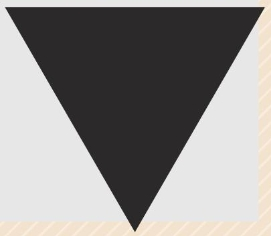
\includegraphics[width=0.7\linewidth]{9}
	\caption{}
	\label{fig:1}
\end{figure}

\subsection{女女这样爱}

女人高喊要性自主,象征要从男性手中拿回性爱主导权,因此,即便没有男人,两个女人也可以一起享受高潮,而已经有男性性伴侣的人,也无妨同时享受女女爱,过程可以更细致、时间更长,相互之间完全没有压力,可以尽情享受,何况“女女爱”还是女性族群中性爱满意度最高的组合呢!

做爱过程中可以播放轻音乐,如法国香颂,再来一点红酒,将是一场如诗如画的绝美飨宴,也可以装上摄影机,全程录影留念。

不管你是“婆\footnote{指气质较阴柔的女同性恋者}”,还是“T\footnote{“Tomboy”的简称,指装扮、行为、气质较阳刚的女同性恋者}”,你们的生理构造一样,观念想法较接近,只要拋开传统成见,就能免除异性伴侣在性爱时经常不同调的尴尬,而享受两人同步达到高潮的极致性爱。

以下是常见“女女爱”的方式:

1.指交:这是最常见女女做爱的方式,透过手指去抚摸对方的阴蒂,或插入阴道,摩擦对方阴道内的G点,让对方达到高潮。

进行指交时,需与伴侣正面相对,手掌朝上,并拢右手中指与无名指(指甲需剪短且清洁过),进入对方阴道后双指微微弓起,大约在入口处往内约3~4公分的位置探索,利用指腹缓缓摩擦,沿着阴道壁左右探索,就可以找到一小块隆起,可能会摸到些许皱褶,这就是G点。

透过持续的摩擦(每个女生喜欢的摩擦频率不同)与观察对方的反应,对方的脸会渐渐潮红、发出呻吟,且会配合摩擦的频率扭动腰臀,当出现这些反应,代表摩擦的位置对了,并且对方快要达到高潮。

在到达阴道高潮时,女生会有全身突然痉挛僵直的情况,并且会有紧抓棉被、枕头或是对方身体的反应,痉挛一会儿后就会突然放松,代表已经达到高潮。高潮的余韻可以维持几分钟,这时两人静静的拥抱就是最棒的ending了!

\begin{figure}[H]
	\centering
	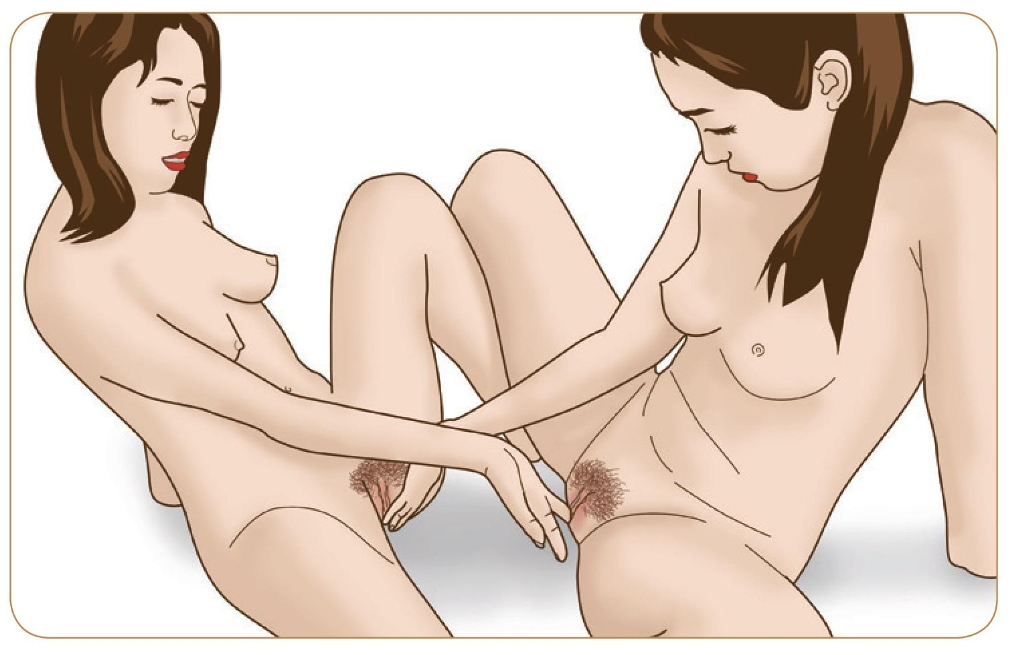
\includegraphics[width=0.7\linewidth]{10}
	\caption{}
	\label{fig:1}
\end{figure}

2.口交:这也是一个可达到阴蒂高潮的方式,其实是透过类似指交,但以舌头来按摩阴蒂,这比手指的触感更为柔软、湿润,感受更舒服。

进行口交时,要让对方正面朝上躺在你面前,让她的双膝弯起,你把头埋入她的胯下,用单手把阴唇拨开,先用一些唾液弄湿她的阴蒂周边,并且透过触、抚、舔、揉等方式,或使用舌尖绕圈,或上下舔,这时要观察对方的反应,因为每个女生觉得舒服的方式不太一样。

什么时候会达到高潮呢?当对方身体的震颤或呻吟越来越强烈,并开始闪躲舌头的接触,就代表她接近高潮了。

3.乳交:让伴侣坐着,你跪在她面前并往前倾,使两人的乳头相触,用你的手搓揉她的阴蒂,再来吻她的乳房和乳头;接下来,你自己往后躺,让伴侣靠在你的身上躺下,你的一支手移到她的阴部,刺激她的阴蒂,同时以另一支手爱抚她的乳头,嘴巴也别闲着,要不时地亲吻她;也可以站在她身后,以一支手为她指交,另一支手揉捏她的乳房,若伴侣很享受,要求她自己抚弄另一边乳房,这样的性爱气氛肯定会很火热。

\begin{figure}[H]
	\centering
	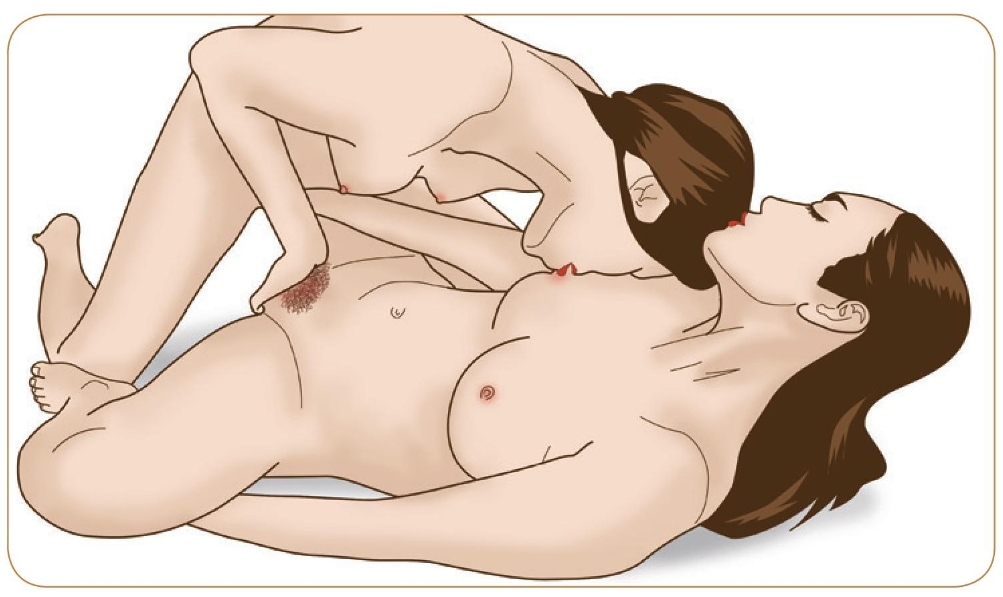
\includegraphics[width=0.7\linewidth]{11}
	\caption{}
	\label{fig:1}
\end{figure}

4.成人玩具:这类选择就很多了,例如用跳蛋刺激阴蒂,或是穿戴上假阳具,空出来的双手可以扶着她的腰,与对方进行超紧密的身体接合。选择成人玩具时只要双方喜欢,样式不必受限,只要能帮助你们达到高潮!

5.剪刀式:这是难度较高的女女爱方法,透过交叉两人的双脚,以私处对私处来摩擦彼此的阴蒂,双方一起扭动腰部,一起达到阴蒂高潮。

\begin{figure}[H]
	\centering
	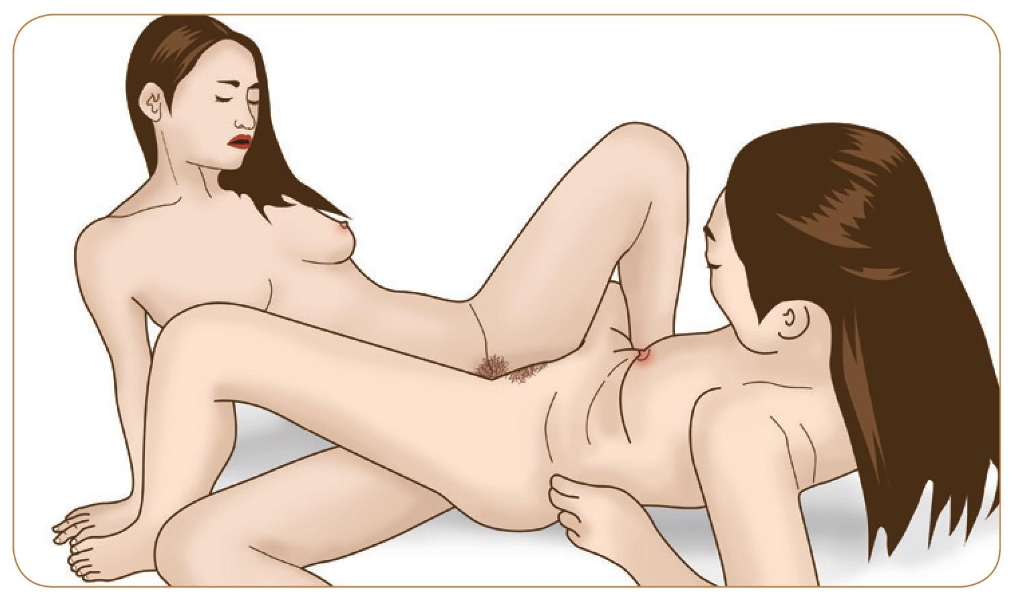
\includegraphics[width=0.7\linewidth]{12}
	\caption{}
	\label{fig:1}
\end{figure}

6.69式:这是标准既可“施”、又可“受”的性爱方式,一方躺下后,抬起双腿,张开,另一方跪趴在上,让彼此的私处与对方的脸相对,这样能更容易刺激阴蒂;要让69式更激情,可以加上手指,使伴侣享受内外都舒适的服务。侧躺也行,两人都躺下后,各自的脸部与对方的阴部相对,各抬起一条腿,其他技巧如上,这样可减少上位者体力付出较多的缺点,保留更多体力,让伴侣享受更多激情。


\part{内衣}

“市场上的内衣琳琅满目,我要从哪里入手才能建立起一个完美的内衣橱?”这是很多朋友问我的问题。当然,还有更多更细的问题,比如:

文胸的棉垫太厚,胸部一看就很假怎么办?

买集中型的文胸,胸是更挺了,可肥肉也被挤出来了,怎么办?

总是被钢圈勒出一道深深的红印,看着就痛,该怎么办?

每次穿运动文胸,脖子都要抽筋了怎么办?

找到喜欢、穿起来既轻松又舒服的文胸真的很困难吗?

……

上面的很多问题都集中在文胸上。


其实,除了文胸,内衣包括的种类还有很多。

经常遇到一些女性朋友这样向我提问:“我的内衣怎么那么不合适,你能不能……”根据她们的语境,我可以立刻明白她们说的内衣其实只是“文胸”。事实上,笼统地把文胸叫做“内衣”的人不在少数,这里面既包括普通消费者,也包括内衣销售员、时尚杂志编辑,甚至我们内衣工作者。

也许是做了多年内衣设计师的缘故,我特别不能容忍有人把文胸叫做内衣,几乎得了强迫症,遇上谁这么说都想纠正。2016 年我在某问吧开了一个专栏,有位提问者对于我的执着很是不满。这让我想起 19 世纪末美国华纳医生的经历。他当年为纠正女性穿过于勒束的束胸衣,一边行医,一边做巡回演讲。可无论他怎么讲,女性也不愿放弃这些伤害身体的束胸衣,于是他干脆自己设计了一款“健康胸衣”,并改行成立内衣公司,即后来美国最大的内衣公司沃纳科集团(Warnaco Group)的前身。

我没有华纳医生的魄力和勇气,只能一遍一遍地提倡“欲立其身,先正其名”,只有先把概念搞清楚才能更好地谈论“内衣”这个话题。

“内衣”一词,工业领域常用的英文是“Intimate Apparel”,实际包括七种类型或至少五种,文胸和内裤只是其中的两种,其他还有睡衣、家居服等。

这五或七种类型也可以简化为两种:一种叫“日内衣”,另一种叫“夜内衣”。这两种足以概括内衣的全部种类,说法简单、易懂,女性朋友们也比较容易接受和理解。

所谓日内衣(Daywear),是指白天穿在外衣下的内衣。包括文胸、内裤、调整型内衣、日内衣背心等,袜类也可以归入日内衣。

所谓夜内衣(Nightwear),则是在以卧室为中心环境的非公共场所的穿着。比如家里既有公共区域也有私密环境,像客厅就是公共的,而卧室则是私密的。又比如在学生宿舍等起居处穿着的衣服等。包括睡衣和居家服。

羞于谈论内衣的并非只有东方人,西方社会也曾有过尴尬于公开场合谈论内衣的历史。羞于谈论,不外乎因为内衣与性有关。20 世纪 50 年代,一位名叫弗雷德里克的美国人第一次在全国发行的男性和女性杂志上做内衣广告,他借用香奈儿的那句名言——“时尚可以消逝,但风格永存”,打出了这样一句内衣广告——“时尚在变,但性永不过时(Sex never goes out of fashion)”。

“性”这个词在当时还是说不得的话题,这句广告语被很多人视为有伤风化。不过它也从此破了大忌,在那之后,谈论女性内衣话题变成一件越来越酷的事情,谁敢谈论谁就被认为很有个性。

说起来,内衣讲究合体以体现女性曲线美,这也是在20世纪50年代才开始有的概念。虽然生产商已经开始生产合体内衣,但是女性并非一下子就接受了要选择“合体内衣”的概念。说来也许你不信,直到20世纪90年代中期,女性才普遍具有了买“合体内衣”这一意识。换句话说,我们的祖母可能一辈子都没穿戴过完全合体的文胸或者内裤。

内衣发展出今天这几个明确的种类,经历了漫长且复杂的过程。从灯笼开裆麻内裤到紧身弹力比基尼,从连体加吊袜带的束腹衣到只遮盖胸脯两个小点的三角软杯文胸,这近百年来走过的每一步都充满艰辛。

我们一直说,一部内衣的发展史其实就是女性解放自己、尊重自己的历史。所以,今天我们在谈论文胸时,如果能坦率地使用“文胸”这个词,其意义肯定大于是否使用了一个准确的词。

现在,就让我们开始了解内衣吧!

\chapter{了解与选购}

关于文胸

Q1. 文胸有哪些种类?

穿戴文胸不仅能美化女性曲线,而且对健康也有好处。可如果使用不当,却会对女性的胸部造成伤害,因此,科学地选戴文胸至关重要。然而,自从文胸进入黄金时代以后,女人们选购文胸就成了一件既快乐又烦恼的事。快乐是市场丰富,可选择的范围大了;烦恼则是市场过于丰富,不免眼花缭乱。而且,虽然有胸型分类,但女性的胸脯仍然太多样化,再复杂的分类也不足以概括所有胸型。那么,如何才能找到适合自己的那一件呢?

年龄、胸部轮廓、季节、社会身份等都可能是影响我们选择文胸的因素。让我们先从这里开始了解吧!

市场上的文胸款式实在是太多了,这些不同款式很难按照某一种规律分入某种类型,即使勉强做出分类,仍是你中有我,我中有你,要想做出十分清晰的分类极为困难。

针对极其丰富、复杂的女性胸脯特征,欧美内衣市场做了一个简便的区域划分:普通尺码(Regular Size)和大尺码(Plus Size)。

普通尺码是指 32AA 罩杯至 36C 罩杯,即国际尺码 80A--90D 。

大尺码是指D罩杯及以上,或38C罩杯起,目前到42J为止,即国际尺码90DD及以上。

现在有一些品牌或内衣公司专做大尺码文胸,但是做普通尺码文胸的品牌和公司仍然占多数。

按照面料分类:

质地平滑的面料,比如真丝面料,包括弹性缎和无弹性真丝等;

普通的微纤维面料,其中有提花或无提花图案;

更为普遍的针织棉面料,其中有带纹路的,也有无任何纹路的。

相对来讲,平滑面料制作的文胸更为实用,它不仅适于任何季节,而且在任何面料的外衣下,即使穿着相当轻薄的真丝或相当紧身的弹性针织面料外衣,这一类面料的文胸也很容易给人安全感。特别是天气炎热时,一件衬垫不太厚的针织棉质文胸是最佳选择,会让人感觉凉爽而舒服。

在我看来,这一类文胸应该是每个女人内衣橱里的必备品,可以每日穿戴。但显然,安全感可能并不是每个女人都需要的,更不是她们追求的终极目标。偶尔改变一下风格,还可以转换心情,这个时候,就需要第二类面料的文胸了。

质地不平滑的时尚面料,如全蕾丝面料、镂空绣花面料、花丝绒面料等。

胸脯是女性最美丽的身体部位,也是最容易被男性注意到的女性特征,对它的爱当然应该表现得更开放、更丰富。况且文胸发展到今天,早已不仅仅是出于卫生和保护的目的了,让女人内心感觉更美好反而更为重要。时尚面料的文胸能充分满足女人的这种心情,因为它们更美观、更性感,即使穿在被人看不见的“里面”,也能让女性时刻感受到“为悦己而容”的满足感。当然,取悦男性并不是最终目的,但客观上,它们的确更容易引起男性的注意和欣赏。

非面料类,如硅胶文胸,现在受到越来越多的人的需要和喜欢。

按照罩杯形状分类:

文胸罩杯款式多种多样,到底什么是“半罩杯”,什么是“全罩杯”,我该如何分清?又怎么知道究竟哪一款适合我呢?这恐怕是很多女性的烦恼。

其实,罩杯有形状区分的多为带钢圈文胸。而因为有钢圈的限制,罩杯不外乎下面五种形状。我们只要对这五种罩杯结构有了基本的了解,再选择适合自己的那一款就会容易很多。

全罩杯(即4/4罩杯)

真正的全罩杯整体呈球状,可将乳房全部包裹在内,能罩全乳房的上半部分。这一种杯型最适合罩杯大或乳房大却扁平、偏软、外扩以及有副乳的女性,也更适合追求穿戴稳固性的女性。

全罩杯从结构上看,有如下几个特点:

1. 罩杯结构上通常有横向杯骨,上碗与下碗的高度几乎相等;

2. 鸡心和侧比位的钢圈较长(如上页红线所示);

3. 罩杯外形通常为高鸡心位(在所有罩杯里是最高的)、高侧比位(侧比钢圈长的结果)、加高夹弯位以及大U型后背;

4. 肩带靠近罩杯的中间,高度从胸部的顶端开始,是肩带开始位最高的一款。

在这款全罩杯的基础上,使用相同钢圈但改变领口形状,就可以变为部分全罩杯款。比如,降低杯口,肩带位置随之改变,往外、往低挪动。



又或者抹去罩杯上端的三角尖角,将罩杯降低成圆线形,随之可以把肩带去掉,变成一款无肩带调整型文胸。其鸡心位置与全罩杯一样不变,但领口调整后更像“方形”,肩带往外挪或完全去掉。



3/4罩杯

通常被称为“Balconette”,最常见的特点是领口呈心形,更多地暴露乳房上半部,有1/4乳房外露。3/4罩杯是现有罩杯形状里聚拢效果最好的。如果你想要明显的乳沟,这款罩杯肯定是首选。适合穿在低领或方领的外衣下。


3/4罩杯的结构有如下特点:

1. 鸡心位较低,低于侧比位;有不同的鸡心高度,但通常在全罩杯与V罩杯之间,比全罩杯低,比V罩杯高;

2. 通常罩杯有上碗和下碗两部分,上碗部分比下碗部分小;下碗部分通常再分两到三块,与上碗部分的杯骨线方向相反,同时有横向和竖向杯骨(如下图)。通常杯骨越多,越能贴合人体曲线,领口也就会越服帖;

3. 如果肩带连接到罩杯的下碗部分,内插棉倒立或斜放,受力点就落在肩带上,能给予胸脯最大的承托。



半罩杯(即1/2罩杯)

通常被称为“Demi”,Demi的意思是“部分”或“一半”,即罩杯包容乳房乳头以下的一半(包括乳头),露出乳头以上的部分。

半罩杯通常罩杯口开位较低,领口呈方形,因此会造成乳沟效果,特别适合乳房娇小及两胸之间距离较大的女性。半罩杯文胸虽然有一定的宽侧比侧收设计,但没有夹弯位,因此不适合胸型外扩、腋下有副乳或赘肉的女性穿戴。


半罩杯的典型特点如下:

1. 通常鸡心部位的钢圈与侧比位的钢圈高度相同,且鸡心位比3/4罩杯低;

2. 通常有竖向杯骨,如果是大罩杯,会有两条竖向杯骨;有时也可能是一条横向,或一条横向加一条竖向杯骨(如下图)。只有一条横向杯骨时,上碗比下碗小,鸡心位更低。

从制版角度讲,使用竖向杯骨是有因为能够更容易制造出一个更低、更开的领口形状,同时让下碗更浅,这样就可以把乳房推高。



1/4罩杯

罩杯低于乳头。有时被误称为半罩杯,实际比半罩杯还要低。



V罩杯

V罩杯文胸与全罩杯很像,但它在两个罩杯间做出一个明显的V型领口,是制造乳沟最好的款式。


V罩杯的结构特点如下:

1. 杯口通常呈斜线,是所有罩杯里钢圈最短的一个款式;

2. 鸡心位很低,尤其如果是聚拢型文胸,可能只有一根底围橡筋的宽度;

3. 如果是背心式文胸或三角软杯文胸,通常没有鸡心位;

4. 罩杯有两条或一条杯骨。有两条杯骨时,通常是一条斜向杯骨与一条竖向杯骨。只有一条杯骨的话,通常是竖向的。



总之,罩杯形状的不同,其实是造成了领口形状的不同。因此,要分清带钢圈文胸的罩杯形状,我们只要看看下面这张领口对比图就一目了然了。

左侧从后往前依次为全罩杯、变异全罩杯、3/4罩杯、1/2罩杯。右侧从后往前依次为全罩杯、V罩杯。



按照功能分类:

实用型:着重吸汗、保护、卫生等基本功能。

品味型:偏向流行、个性、设计等。

功能型:辅助修饰身材某处特定的小缺点。

调整型:强调曲线雕塑,需长时间穿着来达到改变身材的目的。

©EMILY YU工作室





Q2. 钢圈真的能托举乳房,防止它们下垂吗?


类似这样的疑问从钢圈出现就没有断过,而且观点还经常正反相对。有人会问:钢圈真的能托举乳房,防止它们下垂吗?也有人问:长期穿戴无钢圈文胸会让乳房的边际模糊吗?实际上,针对这两个问题,至今尚无科学而明确的答案。

曾有位运动医生对一组自愿不戴文胸的女性进行了多年的跟踪调查,他得出的结论是,这些女性的胸并没有下垂,反而比戴文胸的对照组还更坚挺一点。


除了钢圈是否能防止乳房下垂的争论之外,另一个呼声最高的问题就是钢圈是否有害健康,是否是引发乳腺癌的罪魁祸首。1990年,美国《医学日报》曾发表一篇题为《消灭钢圈》的文章,文章中指出钢圈长期压迫乳腺,阻碍淋巴液循环,从而导致了各种各样的乳房疾病。后来这一观点影响甚广,从医学界到女性社交圈,大家似乎都认同“钢圈有害健康”这一观点,给女性造成了很大的心理负担。

可事实真的如此吗?2013年于《心理肿瘤学杂志》上发表《胸脯高耸》一文的作者格罗斯先生认为这完全是无稽之谈,因为至今没有一项有力证据可以证明乳房疾病与文胸直接相关,无论是因为穿戴文胸还是不穿戴文胸。可是要说钢圈能改善下垂状况,格罗斯先生也并不认同。在他看来,乳房的体积、重量和人体的其他特征一样,是形态演化的结果。也就是说,下垂与否是女性天然身体条件决定的。否则,我们怎么解释为什么有乳房扁平的20岁女性,也有乳房仍丰满坚挺的60岁老太太呢?简言之,格罗斯先生不认为钢圈能起任何作用,无论是好作用,还是坏作用。

其实很多文胸专家都曾提到过一点:感觉乳腺受压迫并不是因为穿有钢圈的文胸,而是因为穿了钢圈不合适的文胸。可事实上,真正对这个问题加以关注的女性并不多,大多数女性在穿戴文胸上都存有误区。


女性要根据自己的年龄和胸部发育阶段选择是否穿戴有钢圈的文胸。如果是正在发育的年轻女孩,乳腺不能受到过多压迫,就应该选择无钢圈或软钢圈的文胸;但是要根据胸部的发育情况及时更换文胸,发育到一定程度之后就应换上有钢圈的文胸,以防止胸部下垂的情形出现。如果是已经发育成熟而身材仍十分娇小的女性,因为对于承托的要求没有丰满的女性那么高,可以多选无钢圈或软钢圈文胸。

这里要纠正一个选择误区:不是穿有钢圈的文胸就会压迫乳腺,大部分是因为穿错才压迫。





Q3. 常见的无钢圈文胸有哪些?


硅胶文胸

硅胶文胸通常无后背、无肩带,只有两个由硅胶制成的罩杯,罩杯内涂有医用级别的黏胶,可以直接贴在乳房上。

我们大概都有过这样的经历:今天想穿某一款露背装或抹胸裙,可试遍了所有的文胸都不合适,不是露出了不该露的肩带,就是露出了背钩……这个时候,硅胶文胸就是最佳的解决方案。每位女性都需要为自己备上一副硅胶文胸,因为它能在你想要充分展现性感时,给乳房最好的支撑和保护。

造型式文胸

也称为“魔杯式文胸”。用一体式热压模杯制作的文胸,具有突出和定义胸部轮廓的功能。由于模杯通常用海绵或填充纤维制作而成,有一定厚度,故绝对不会出现露点情况。

此款文胸会使胸型看上去绝对圆滑和对称,因此特别适合两胸不对称的胸型。但它并不会让胸部看上去更大。

无缝式文胸

又称“一片围”。半无缝式,又称“半片围”。

所谓“一片围”,就是除去肩带以外,罩杯、围度、背钩等完全是一体成形,无拼接缝。罩杯通过所谓的“子弹头”冲模技术高温定型,呈现3D立体效果,让胸部自然丰满盈润。罩杯厚度可控,通常在1.5厘米左右,上薄下厚。肩带较宽。

所谓“半片围”,就是在侧比有接缝,围度一体成型。这款文胸特别适合搭配T恤,或布料较为柔软光滑(如丝绸)的外衣,或紧身的弹性针织外衣。

抹胸

又称“一字文胸”或“裹胸”。抹胸是最简单的文胸款式,用一块布围在胸部而成。这种文胸几乎没有支撑力,因此只适合小胸女性。

胸衣

通常是用蕾丝制作的无钢圈、无胸垫的整体舒适胸衣,集运动、休闲与时髦元素于一体,既可以内穿,也可外穿出街。

胸衣没有塑形、支撑的功能,所以更受拥有小巧、坚挺胸型的年轻女性欢迎。不过也正因为它不能制造集中、深V、高耸等效果,呈现的是自然状态,深受崇尚天然的时髦女性的追捧,因此经常被套在外衣下外穿出街,或内搭在比较宽松、随意的外衣或睡衣下暴露出来。

胸衣常见三角软杯设计。内穿的三角软杯现在大多配有小插片,可以根据自己的需要装卸以避免凸点。如无插片口袋设计,就需要佩戴乳贴。





Q4. 选择钢圈文胸时,底围和罩杯总有一个不合适,该如何解决?


这种底围和罩杯总有一个不合适的情况分为很多种。

钢圈部位的底围合适,罩杯却总是过小;如果选择合适的罩杯,底围又会过大。

这种情况通常出现在乳房D罩杯或以上的女性身上。这种胸型通常被称为“球形胸型”,胸围从底部到乳头处不是像其他胸型那样越来越小,而是越来越大,甚至溢伸到身体躯干以外。

形成这种胸型的原因很多,常年穿着不合适的文胸可能是主因。比如,文胸质量差,没有足够的支撑;经常不穿文胸;体重长期频繁增减;常年穿戴错误尺码的文胸等。当然,也有天生如此的胸型,比如发育过快或过于成熟的年轻女性。


文胸款式推荐:

1. 最好的选择是裁剪缝制一体化的文胸。这类文胸通常是立体裁剪,完全按照胸部曲线拼缝制作而成,能形成非常贴合胸部线条的圆弧形。罩杯可以由两块或多块布料组成。通常接缝越多,支撑力度越好。

2. 选择罩杯使用非弹性布料的文胸,能更有效地支撑乳房,使其不会轻易晃动。

3. 选择带有侧翼胶骨的文胸,这个胶骨可以对乳房起到一定的固定作用,使乳房保持在身体前方和中间,而不是向身体外侧溢出。

4. 全罩杯当然是极其必要的选择。

5. 深V型文胸也是一个不错的选择。

6. 不要选择轮廓式模杯文胸,除非模杯是由大尺码文胸专制公司出品的。一般的模杯是不可能给这种胸型以足够正当的支撑的,也不可能合体。


钢圈总是显得过宽,老往下滑。

那是因为你的胸型是我们常说的“薄胸型”。C罩杯以下的小尺码胸常见此类胸型。

通常这种胸型乳房下围较小,两个乳房之间距离较大。这种胸型还会经常遇到乳房不能把整个罩杯撑满的情况。


文胸款式推荐:

1. 不建议选择一般的钢圈文胸,它们不可能合身,而且钢圈的位置不合适还有可能伤害到你的胸骨。

2. 软杯文胸(没有钢圈)会比较舒服,但无法体现出比较优美的胸线。罩杯可能撑不满,可用活动胸垫弥补。

3. 推高式文胸比较好,能让胸型显得丰满。

4. 在底部和罩杯外侧带胸垫的推高式文胸最为合适。

5. 在罩杯底部使用活动式衬垫,会让你的胸型更为丰满。

6. 由较硬的模杯制作而成的轮廓式文胸也是一个不错的选择,能让你的胸型看上去更圆满一些,也可以掩盖乳房不能充满整个罩杯的缺陷。

7. 深V型文胸也可选择,但要选择中间钢圈位置较低的款式。


文胸底托很合适,罩杯却不能被撑满。

这种情况经常出现在胸型较小的人身上。胸部底围足够圆润,可是胸很小,这样的胸型被称为“锥体胸型”,近似冰激凌蛋筒的形状。市面上的文胸一般是按比例进行设计的,对于这样的胸型来说,通常选择合适的底围后,罩杯就会太大,出现空杯现象。


文胸款式建议:

1. 轮廓式模杯文胸是这种胸型最好的选择。左右罩杯之间的连接部分较高,罩杯底部如果有加厚则更好。

2. 可以在罩杯的底部放入活动式小棉垫以衬出胸线,填满罩杯。

3. 底部加厚的推高式文胸可以从底部和两侧往上推挤乳房,使胸部看上去更丰满,还有可能造成乳沟。A罩杯或B罩杯的小胸可以选择底部加厚的推高式文胸。

4. C罩杯或更大罩杯,应选择“轮廓减小式文胸”,它会让你的胸部看上去更圆满,但又不会过于丰满。

5. 最好不要选择软杯或没有任何结构支撑的文胸。它们没有塑形功能,会让你的胸线毫无魅力。





Q5. 有哪些特殊的功能性文胸?


运动式文胸

运动文胸不仅仅是比普通文胸增加了支撑力,而是在女性运动时,尤其是做前跃或跳跃动作时,对胸部韧带和软组织加以保护。

运动文胸的设计原理是尽可能固定住两个乳房减小其晃动幅度,减小女性运动时的痛苦和烦恼。

随着人们运动意识的提高,运动已经成为女性日常生活中十分重要的事情,运动文胸也成为女式内衣中十分重要的一个品类。

T恤式文胸

T恤式文胸剪裁与半罩杯或全罩杯一样,通常使用平滑面料或无缝模杯。线条简洁流畅,穿在T恤下不会露出文胸痕迹。

T恤式文胸是搭配在针织衫(包括T恤衫、轻软的毛衣)和紧身衣裙最理想的文胸款式。

孕妇文胸

孕妇文胸的设计具有较强伸展性,以适应女性在怀孕期间胸部尺码的不断变大。

哺乳文胸

哺乳文胸的设计是为方便产妇授乳,让婴儿更容易接触到母亲的乳头。传统上,哺乳文胸上有一块可以从上端揭开的布,翻下来就可以露出乳头,方便哺乳。

轮廓减小式文胸

特别为34C罩杯以上的胸部丰满女性设计,通过压平、均摊乳房纤维等方法,可达到视觉上减少1~2个罩杯尺码的效果,让胸部不会显得过于丰满。而且这种文胸普遍更为舒适。





Q6. 你喜欢多厚的胸垫?带垫还是不带垫?


走进国内的内衣店,常常看到的大约只有两种风格:一种是上面附着大量刺绣的厚模杯或厚棉垫款;一种是老气横秋的调整型。无论哪一种,其实都是为了让胸部看上去更大、更挺,以挤出“事业线”为目的。

可这是你希望的吗?

海绵模杯是从西方来的,最初面世时的确引得无数女性为之着迷,又被称为“魔杯”。不过,这样的厚杯或厚垫文胸在今天的欧美内衣市场早已不是主角。随着女性自我意识的提高,不要说厚模杯,就是厚海绵垫也开始因为效果虚假而遭到她们的厌弃。它们开始变薄,从全罩杯加厚模杯变成只有罩杯下半部分加厚;形状和大小也发生变化。如果原先的罩杯是棉垫设计,一定会占满整个罩杯,现在即使是全罩杯设计,胸垫也可以只占罩杯的一半,甚至更少。今年我甚至看到过只占三分之一罩杯的杯垫设计。欧美市场意识到,或者希望消费者意识到,胸垫其实只要能够遮点就足够了。

其实如果问现在的国内女性:“你喜欢多厚的胸垫?”恐怕有不少人的回答会是:“薄薄的一层就好。



太厚的胸垫除了能塑造“波涛汹涌”的效果以外,跟薄杯比,对胸部的保护并没有什么特别,只会让我们感觉虚假而不安。可是如果罩杯完全没有棉垫,只是薄薄的两层布,我们又会有凸点的担心。所以,不超过1厘米厚的棉垫我觉得恰到好处。希望我们的市场可以有更多这样的设计以满足女性的需求。说到底,内衣市场终究是为女性服务的。

文胸的海绵是通过压模成型的。一般有三层材质,最外面上下两层贴布,中间通常是聚氨酯海绵,也是常说的普通海绵。处理时会加一些抗黄棉,防止海绵发黄。海绵的厚度可以按照设计师的要求制作。质量好的海绵具有良好的透气性,吸汗能力强。前两年直立棉也曾风靡过,但直立棉与聚氨酯海绵究竟哪个更好,一直存在争议。

最外面的上下两层贴布,通常是用全涤75D佳积布;要想手感再细腻柔软一些,则用50D佳积布。质量再高的,则用全棉或T/C涤棉布。

不过,到底是要穿带垫还是不带垫的文胸,纯属个人喜好。

在过去一二十年里,大部分中国女性比较追求聚拢、高挺的效果,所以市场上绝大多数文胸都是带有棉垫的,而且是比较厚的棉垫。而现在,特别是最近一两年,棉垫的薄厚出现了更多的选择。有热压一体模杯、子弹头冲绵垫和车缝棉垫等,每一种的薄厚都有不同。有整个罩杯同一厚度的,也有底部半杯加厚的,而棉垫的厚度的选择则更自由了。

棉垫薄厚的变化,也反映了女性对待自己身体的态度变化。

如果你的乳房有一大一小的现象,那选择一体模杯是最合适的。如果希望自己的胸看上去更大,那选择有聚拢效果的带厚垫文胸也无可厚非。可如果你希望自己的胸既受到足够的保护又能保持自然的状态,那么1厘米厚的车缝绵垫就是非常好的选择。





Q7. 什么是软杯文胸?适合什么胸型的人?


所谓软杯文胸,就是没有钢圈、没有海绵垫,通常只有薄薄两层布料的三角杯文胸。外形和比基尼泳衣的上衣很像。

这种文胸因为罩杯柔软、对胸部没有束缚,会让穿着者感到放松自在。不过也正因为只有薄薄两层布料以及对胸部的束缚和支撑不够,所以它更适合罩杯34C/36B以下、乳房小而坚挺的女性。比这个尺码大的胸型,乳房就很难被三角杯承托住,因此不建议购买、穿戴。





Q8. 胸型是怎么分类的?


市场上标准化的文胸结构设计会针对不同胸型设计制作不同的款式。就是说,某些款式肯定更适合某种胸型,某些胸型不适合穿某种类型的文胸。我经常听到身边女性朋友抱怨自己遇到的问题,这些问题也是其他女性经常遇到的,究其原因就是她们穿上了不合适的文胸。所以,了解自己的胸型是找到对应文胸款式的第一步。

娇小胸型

娇小的胸部,最容易用文胸来进行弥补。对于胸部娇小的女性而言,下厚上薄的3/4罩杯文胸能集中托高胸部,塑造丰满、自然的胸部曲线。但如果胸部尤为平坦,那全罩杯则是最佳选择,全罩杯的密合度较佳,弯腰时不易发生空罩杯的情况。



另外,小胸女性也不要因为胸部小而选择过紧的文胸,略大一点的文胸才能让胸部血液顺畅流通,并且给予它朝合适的位置发展的空间。如果你希望胸部显得更丰满,应首选轮廓式模杯文胸;如果你不在意大小,可以选择三角软杯文胸,当然最好配一副活动式棉垫。

丰满胸型

C罩杯以上便属丰满胸型,丰满胸型要保持挺实、不下垂、不外扩,选对文胸是关键。身材丰满的女性宜选择轻薄的丝质面料文胸,最好不要选有棉垫的文胸,V罩杯和3/4、4/4型都比较适合此类胸型。另外,宽肩带加钢圈,也能更好地支撑胸部的重量。

下垂胸型

胸部下垂的女性,应该选择无弹性全罩杯以加强胸部支撑,肩带与后背带也都需选择较宽的款式,并尽量使用钢圈和侧部有加强功能的文胸,使之加强衬托,由下往上地支撑,才能将下垂的胸部承托起来。



乳房有副乳型

有副乳的女性应该正确选择聚拢、软性布料加强文胸,从而达到胸部向内聚拢的效果。后背扣与前肩要相配合,并尽量穿戴带有固定型钢圈功能的文胸。整个文胸应全部托起胸部并包裹住乳房,这样才能支撑、聚拢、调整副乳。





Q9. 应该在什么时候购买人生中第一件文胸?


生活中,不少人认为到了16岁或者乳房隆起就应及时穿戴文胸,但这并不科学。


事实上,不管你多少岁,只要看到自己的乳房开始隆起,就应该拿起软尺从乳房的上底部经过乳头到乳房的下底部进行测量。如果测量出的数字大于16厘米,那你就应该穿戴文胸。如果年龄大于16岁而测量结果还是小于16厘米,则仍然不宜穿戴文胸。因为过早穿戴文胸不仅对正处于发育隆起的乳房不利,而且还有可能影响以后的乳汁分泌。

也就是说,何时购买人生中第一件文胸,不是根据年龄,而是根据乳房发育的速度和大小来决定的。而乳房的发育受遗传、营养、运动等各种因素的影响,每个人的状况都会有所不同,因此需要对自己的身体保持敏感并加以科学的认识。


一般而言,大多数女孩在长到16~18岁时,胸廊和乳房的发育会接近成熟,所以,这也是我们通常提倡的开始穿戴文胸的年龄。

但有一部分人会觉得“虽然我的乳房已经发育成熟,可我不想穿文胸”。可是这样好吗?

当然不好。乳房在充分发育后就需要加以保护,否则日常行走、运动和劳动等都有可能使乳房因过度晃动而造成伤害。乳房是人体少有的没有肌肉的器官,胸部韧带一旦受伤不仅无法修复,而且也无法通过任何方法再得到加强。

所以,及时穿戴文胸是保护乳房最简便的方法。

除了减少伤害,文胸还可以托起并支撑乳房,使其血液循环通畅,有助于乳房的进一步发育。





Q10. 第一次购买文胸时,应该做些什么准备?


首先要学会测量自己的胸围尺码


测量上胸围

上身前倾45°;

软尺绕过乳点一周,得出上胸围尺码。


测量下胸围

身体直立,软尺贴近乳根;

水平环绕一周,得出下胸围尺码。

了解计算罩杯尺码的公式

罩杯尺码=上胸围-下胸围。

上下差若在10厘米左右为A罩杯,在12.5厘米左右为B罩杯,在15厘米左右为C罩杯,在17.5厘米左右为D罩杯,在20厘米左右为E罩杯,在22.5厘米左右为F罩杯,以此类推。

有了这个公式以后,就能轻松得出自己比较确切的罩杯尺码了。

如果你的下胸围是75,罩杯为B,对应的文胸尺码就是75B。





Q11. 如何看懂文胸的尺码?


如上所述,罩杯尺码通常由一个阿拉伯数字和一个字母组成。这两个数据看似简单,但对女性朋友而言是选择文胸十分重要的依据,需要牢牢记住。

用阿拉伯数字表示的底围尺码永远不变

也就是说,一旦找到最合适你、让你感觉最舒服的底围数字,比如75或80,那么你看中任何品牌的任何款式,你都可以自信地选择那个数字。因为对于任何款式来说,无论罩杯如何变化,底围的长度都是不变的。举例来说,75B的底围长度与75C或75D的底围长度没有任何不同(如下图)。



罩杯随底围尺码变化而变化

文胸罩杯的容积因为底围增加而增加,比如同样都是B罩杯,70B<75B<80B。看上去似乎变化的只是底围尺码,实际上罩杯容积也发生了变化。因此,如果文胸底围尺码发生了变化,你就需要调整你的罩杯尺码(如下图)。



不过,请永远记住一个终极原则:合适才是一切!





Q12. 有关文胸结构的名词有哪些?



Column

了解这些名词,对了解复杂的文胸结构很有帮助,我们在实体店选购时能更容易与店员沟通,特别是在电商平台上选购时会更容易理解款式描述,有助于我们选购到合适的文胸。

不过有关文胸结构的名词实在很多,如果不是专业设计师或生产人员没必要全部知道,只需掌握下面这几个名词的概念即可:



1. 鸡心:又称心位、前中位。

2. 侧比:又称侧翼,是后比与罩杯之间的连接结构部分。

3. 夹弯:又称比弯,是罩杯靠近手臂的位置,起到固定、支撑和包容副乳的作用。

4. 后比:又称后翼或后拉片。

5. 上托:又称上碗,是罩杯的上半部分,通常是一整片。

6. 下托:又称下碗,是罩杯的下半部分,有一片、两片或多片之分。

7. 杯骨:连接上托和下托的那条线。

8. 胶骨:连接后比与侧比的结构。通常是细窄条的塑料制品,有一定韧性,可以支撑侧比,使其不起皱、不变形。

9. 背扣:又称钩扣,可以调节下底围的长短。





Q13. 买文胸一定要试穿吗?


当文胸只有实体店单一销售方式时,试穿曾是自然而然的事,没有人对此有所怀疑。

市场上的文胸款式很多,又有很多不同的品牌生产商,即使是同一个尺码,不同款式、不同品牌也会有所差别,做不到只要尺码一样就全都合适。而且你自己的身体也在不断变化中,以前尺码合适的文胸很有可能过一段时间就变得不合适了。因此当你在实体店里购买文胸时,一定要试穿!试穿除了要试你平时穿的尺码,最好再多试几个与其相近的两个尺码,这样才能知道到底哪一个最适合自己。

如果不知道自己的尺码,可以在买内衣的时候让导购帮你测量一下。

不过现在很多的内衣品牌在电商平台做生意,有些内衣品牌并没有实体店,基本没有试穿文胸的机会。那该怎么办?

首先,最好选择能提供多种尺码标准的内衣品牌。如果是文胸,尺码应不只是简单的S、M、L,而是有更详细的罩杯尺码分类,比如从70到85、从AA到EE等。

其次,最好选择能提供详细购买指南的内衣品牌。为了让消费者不经过试穿就能买到合身的文胸,这些内衣品牌通常会下很多功夫,用数据和绘图给出非常详细的选购指南,你只需要依照“量体指南”认真测量自己的胸围即可,一般都能买到比较合身的文胸。





Q14. 两个胸大小不太一样正常吗?该如何选择文胸?


正常。这世上没有一对乳房是一模一样的。

也就是说,没有两个女人的胸是一模一样的,同一个女人的左右两胸也不一样。可能一侧稍大,一侧稍小,左右差在一个罩杯尺码之内;可能一侧稍高,一侧稍低;乳头的大小也可能不同,凸出的方向亦会有细微差别。

因此,在确定了胸型以后我们还有一个工作要做,就是确定自己两个乳房的差别有多大。

在选择文胸时,我们应该根据较大的那个乳房的尺码进行选择,用其他辅助手段弥补偏小那个乳房的不合适。比如,如果乳房小的一侧产生空杯现象,可以在那侧罩杯里使用活动式棉垫。

两个胸的大小差别如果是在一个罩杯尺码内,穿模杯文胸便可以弥补缺陷;如果差别太大,就需要私人订制合适的文胸了。





Q15. 不同年龄阶段的人应该如何选择文胸?


少女时期:应注重保护性和支托性。讲究舒适性、吸汗、辅助塑造初期胸型。通常款式有AA系列、背心围等。

青年时期:应注重保护性和美化性。可以修饰胸部、增加美感。通常有蕾丝花边系列、轻型收束系列。

中老年时期:注重保护性和修身性。通常有全杯型、中型、重型收束系列。或注重保护性和保健性。通常有无钢圈系列和轻型收束系列。

少女时期

对于青春期的少女来说,选对文胸可以为未来的乳房发育打下重要基础,所以万万不能马虎。

这个时候选择的文胸不能过紧,也不能过松。有些女孩发育比较成熟,但乳房体积较小,这类女孩常犯的错误就是选用很宽松的文胸或者干脆不穿文胸。这样会使乳房失去依托,虽然还不至于下垂或者变形,但为未来的发育埋下了不小的隐患。

少女还处于未完全发育的阶段,日常运动量又比较大,文胸应选择柔软、透气好、散湿性强的材质。

虽然棉布是公认的健康材质,但对少女并不适合。因为棉布吸湿性太强,又无法速干,日常运动量大、出汗多的少女穿着可能会很不舒服。因此应选择优质的弹力化纤面料,比如锦氨、尼龙等,或这些成分含量较高的面料。

还在发育阶段的少女不宜穿戴有钢圈的文胸。


对少女来说,最近市场上大热的用贴合工艺制作而成的无痕背心围,是非常合适的款式。背心围在胸部用一种叫“子弹头”的磨具冲出一个凸起的空间,形成可扩展的弧度空间,很适合青春期乳房快速发育变化的需要。这个凸起的空间通常有两层,在背面有可以装棉垫的口袋,需要时可以插入活动式棉垫,对乳头加以保护,也防止凸点的尴尬。

青年时期

对这一年龄段的女性来说,选对文胸就像选对结婚对象一样重要。事实上,市场上大部分的文胸产品都是为这个阶段的女性提供的,几乎所有的款式都可以在她们的选择范围内,比如钢圈、模杯、插片文胸等,她们有充分试穿、找到最适合自己那一件文胸的机会。

对她们来说,理想的文胸应该是在人体活动时刚好能托起乳房,能尽量限制乳房的活动而不影响呼吸,取下后皮肤上不会留有压迫的痕迹。同时,美感在这一阶段也格外重要,因为这是她们人生中最美好的年龄段,选择文胸尽可以大胆、前卫,给自己的身体以充分展示的机会,不留遗憾。

因为此时女性的乳房已基本完成发育,文胸的大小以完全贴合为最佳。过小,会压迫乳房和乳头,影响呼吸,使乳房感到不适;过大,则达不到支撑、保护乳房的作用,也会严重影响美观。

这一阶段的女性大多会经历哺乳过程,有穿戴哺乳文胸的需求。如何选择哺乳文胸,后面会特别讲解。

中老年时期

这一年龄段的女性身体普遍“发福”,大多需要穿超大尺码的文胸。

在欧美国家,有一个专门供给大身材的文胸区域叫做“Plus Size”,目前,在市场上所占的份额也越来越大。

与普通尺码的文胸相比,大尺码文胸显然更注重功能性,焦点集中在“罩全(Full Coverage)”和“推高(Push Up)”上。中老年文胸市场上可以矫正下垂的全罩杯款式居多。全罩杯式大多有钢圈,或者底围用较宽的橡筋,这些都是防止下垂的重要设计。大尺码文胸最好是宽肩带的,一般应不窄于2~3厘米。因为乳房有一定重量,只有足够宽的肩带才能给予足够的支撑,否则很容易造成肩背疼痛。如果肩带不够宽,可以购买加宽的肩带。



拥有大尺码乳房的女性常常对文胸有更多、更高的要求,可是我们也注意到,市场上适合这部分人群的文胸跟普通尺码比,款式少很多,美观度也低很多。我常常听到大罩杯女性对此事的抱怨,也常常收到私信问我为什么不能为她们设计更为美观的文胸。因为文胸设计特别受技术的影响,大尺码的文胸在功能性方面有格外要求,尤其有赖于技术方面的支持。比如,如果能出现新的弹力布料,或是更符合人体力学的模杯、钢圈,甚至研发出功能创新的肩带、围带、背钩等,这部分设计就能出新。否则,就很难在美观和功能并重上有所突破。





Q16. 底围只有70,可罩杯却是E,应该如何选择文胸?


底围小,罩杯大,多出现在发育特别成熟的年轻女性身上。

这种胸型需要选择罩杯尺码分类更为细致、丰富的文胸款式,如果尺码分类仅有S、M、L肯定不合适,一定要选按照罩杯尺码分类的文胸,比如A杯从70~90都有,或者从70A~70E都有的类型。

不过,因为尺码分类越多就越容易造成库存积压,所以一般品牌都不愿意这么做,市场上只有为数不多的一两个品牌肯这样冒险,这类胸型要选择文胸有很大困难。有的人只好买来罩杯合适的文胸,然后自己改短底围,或者私人订制。





Q17. 文胸穿上后,总是塌陷着、皱皱的,应该怎么办?


这种胸型的形状很像投影效果,即有着合适的底围,但乳房却没能充满整个文胸的罩杯,这种胸型叫做投影渐小形胸型。


文胸款式推荐:

1. 首先应选择钢圈胸围尺码合适的文胸,然后借用强化胸部的配件,比如活动式棉垫之类,填充罩杯里面的空隙。

2. 选择使用弹性布料制作的罩杯,可以根据胸型自行调整松紧度。

3. 选择罩杯上端有弹性橡筋带的文胸。

4. 轮廓减小式文胸可能是非常好的解决办法。这种文胸的罩杯通常在设计时就会把这个问题考虑在内。





Q18. 罩杯大但不想显得太丰满,应该如何选择文胸?


你可以选择模杯文胸,不会再增加胸部尺码。也可以选择减小胸型式的文胸,这种款式的文胸通常是将胸部推高,再分散胸部纤维组织,以便让胸部看上去不再那么突出。

或者选择有运动风格的文胸,这样也可以给肩膀和下围更好的支撑。





Q19. 明明是A罩杯,需要把自己穿成C罩杯吗?


当然是完全不需要。

且不说市面上那些为了让A罩杯或AA罩杯显得更丰满而设计的文胸有多可笑,垫那么厚的垫有多不自然。如果我是个纤细苗条、四肢修长的人,A罩杯对我来说,不但不减分反而是加分。它们让我更轻盈,更飘然似仙,周围的女性朋友们不知有多少都在羡慕我呢。

其实A罩杯真的有很多令人羡慕的地方。现在很多网络论坛上都有类似“平胸女人更美丽”的话题,网友们总结出了A罩杯的种种好处,不是“酸葡萄”,更不是自欺欺人。比如,跑步或跳舞时乳房不会因为晃动而疼痛;睡觉姿势可以更加随心所欲,趴着睡也很舒服;而最让小胸女性开心的是,最困扰那些大胸女性的下垂烦恼,A罩杯完全没有。

早几年欧美已经出现了“我是平胸我骄傲”“平胸女联合起来”诸如此类的互联网群组,还有像“胸小心大”这样的命名网站。参加这些群组的人,对市场上销售的内衣提出的口号是“你驾驭得了我(的乳房)吗?”而不是“我(的乳房)够大(穿你)吗?”

她们不再在乎女性内衣是不是能把自己的胸衬托得更大,而是呼吁设计师们设计出更多适合自己自然身体状态的内衣,比如三角软杯、不带海绵垫的单层文胸等。

其实不止欧美,娇小身材居多的国内也能听到越来越多的“A罩杯也不错”的说法。胸小怎么了,没有乳沟怎么了?很多小胸女人要不是需要上班,会议室总是冷气过量会造成“凸点”,她们不穿文胸也觉得没什么,是否是A罩杯更无所谓。

这当然是勇敢前卫的观点,尤其现在仍然有那么多形容A罩杯的词,比如“一马平川”“飞机场”等。即使不说充满恶意和鄙俗,也肯定不是什么好意。敢于接受自己的真实,认可自己的不完美,其实是更完美的美。

选择穿什么样的文胸,是由你对待自己乳房大小的态度决定的。





Q20. 你应该有哪些颜色的文胸?


文胸抽屉里,平滑面料和非平滑面料的文胸应该占比差不多。平滑面料因为其基础性,以素色为主,黑、白、肤三个基本色是必备,最好也有一两件炭灰和花灰色。同时,每个季度可增加一款流行色。

非平滑面料的文胸,比如蕾丝、刺绣文胸等,颜色就可以比较大胆和开放,多以流行色为主,或者完全不考虑流行颜色,选择自己钟爱的就好。

©EMILY YU工作室





关于内裤


内裤是女性最重要的贴身衣物,因为直接跟身体最敏感的部位接触,所以选择一款好的内裤对女性来说可能比选男朋友还要有挑剔精神。那么,要怎么挑选适合自己的内裤呢?





Q21. 常见的内裤材材质有哪些?


棉

棉的种类很多,包括棉花的棉,各种天然纤维织就的棉,比如莫代尔棉、匹马棉、竹纤维棉等,还有备受推崇和青睐,价格也比较高的各种有机棉。

棉质具有很好的亲肤性,很少有人会对棉质过敏,因此,我个人认为内裤最好的材质是棉,建议每个女性的内裤抽屉里,以棉质为主的内裤起码应该占一半比例。

弹力色丁

通常表面光滑,有亮度,背面暗沉。其原料可以是棉、混纺、涤纶、纯化纤等。色丁被注入氨纶丝的面料就是弹力色丁,光泽度、悬垂感都很好。轻薄柔顺,抗撕裂度高,丝绸手感,品质高雅。

也有真丝弹力色丁,但价格十分昂贵,只有高端品牌才会使用。

弹力色丁虽然有一定弹力,但如果用在整条内裤上还是会有弹力不足的问题,因此弹力色丁通常会混搭其他材质制作内裤,比如弹性蕾丝、弹力网纱等。

蕾丝

又称花边,是一种网眼组织,最早用钩针手工编织。

蕾丝使用尼龙、涤纶、棉、人造丝作为主要原料,如果加入氨纶或弹力丝即可获得弹性,成为弹性蕾丝。

内裤上常见的弹性蕾丝类型如下:

尼龙(或涤纶)+氨纶:常见的单色弹性蕾丝;

尼龙+涤纶+氨纶:由于在锦和涤纶上染的颜色不同,制成双色蕾丝;

尼龙(涤纶)+棉:可以做成花底异色效果蕾丝;

全棉+氨纶:棉质弹性蕾丝。

弹力网布

通常是针织网布,原料一般为尼龙、涤纶、氨纶等。柔软轻薄,透气性好,弹力大。

微纤维

又称超细纤维。用合成纤维制作的布料,其纤维单位在0.3旦(直径5微米)以下,仅为真丝的1/10。最常见的超细纤维材料是化纤或尼龙,或尼龙和化纤的混合,也就是绦纶和锦纶两种。

超细纤维由于纤度极细,大大降低了丝的刚度,制作成布料手感极为柔软,还有真丝般的高雅光泽,并有良好的吸汗、散湿性。目前,微纤维是制作内衣最流行的材料,成品舒适、美观、保暖、透气,有较好的悬垂性和丰满度,在疏水和防污性方面也比一般纤维要高。

超细莫代尔

由澳大利亚蓝晶(Lenzing)公司注册商标的一种微纤维,用山毛榉纤维素纺制的布料。这种纤维比丝线还精细,织成的布料非常精致且质量轻。用超细莫代尔制作的女性内衣,被美誉为“第一肌肤”,顾名思义,比“第二肌肤”更胜一筹,几乎可以做到没有穿戴痕迹。超细莫代尔表面光滑,可以防止酸橙和洗衣液的沉淀,即使经过多次洗涤后仍然如丝般光滑柔顺,颜色明亮鲜艳。超细莫代尔比棉的吸水力强50%,因此可以让皮肤更好地呼吸。

匹马棉

特指在美国、澳大利亚、秘鲁生长的一种超长短纤维棉,世界只有少数地方可以出产,数量十分有限。匹马棉以前被称为“美国-埃及棉”,后来被重新命名,以奖励在亚利桑那州的撒卡顿为美国农业部种植了这种棉的匹马印第安人。匹马棉与高地棉的主要区别在于纤维的长度和力度。在美国,如果棉纤维长于1.375英寸,就被认为是匹马棉。它的韧度和细度都比高地棉要好。质地自然柔软、手感顺滑,悬垂感特强,织出来的布料韧性十足,价格相应地也比较高。





Q22. 内裤有哪些常见款式?


内裤的款式是经过几十年发展积累而来的,市面上看似种类繁多,令人眼花缭乱,其实大体都可以归入五种基本款式:



经典短裤



内裤中最常见的款式。腰部位于或稍低于肚脐,故分为高腰短裤和低腰短裤。年龄大的女性更适合高腰短裤,因为它对腹部有更好的保护。低腰则更适于年轻女性。跟比基尼相比,它包裹臀部和腿根部更为严实。腿部开口有高开或普通开样式。

比基尼短裤



比基尼短裤是从泳装概念演化来的内裤款式,腰部通常低于肚脐。后来因为出现了超低腰的牛仔裤等裤型,也就有了更低腰的款式。

比基尼短裤的腰围在臀部靠上,腿部有时为高开口,特别高开时两侧可为细带,称为细带比基尼,夏季尤为常见。

臀裤



与臀部熨贴的一款内裤,所以叫臀裤。

这一款式是我最喜欢推荐的,我个人也穿得最多。它的两侧长度其实很像经典短裤,又比比基尼短裤的侧翼长,因此两侧感觉十分妥帖。腿部开口也与经典短裤相像,相比比基尼的腿部开口要低,因此对下腹和臀部都能有足够的包裹和覆盖。

我最喜欢臀裤的一个特点是它的前后腰都有一个往下的弧度,前腰弧度通常更大,后腰也正好在臀围的测量点上或者以下,因此比经典短裤穿上后的感觉要轻盈许多。如果是喜爱运动的女性,特别是腹部较平坦的女性,穿上它应该都会感觉特别舒服。即使腹部不够平坦,穿上这款内裤也会立刻感觉轻便许多。

有的臀裤有前后中缝,尽管它有时看上去的确更漂亮,但如果布料的弹力不够强,会很容易出现夹沟现象,造成不适。所以,尽量不要买有后中缝的臀裤。

平角裤

这是仿男孩短裤款式的女式内裤,但比男孩短裤款式有魅力得多。



有些款式则会特意采用男式内裤元素作为装饰,如前开气效果。



此款内裤侧翼通常很长,能包裹住整个臀部,腿部开口很低,常与大腿根齐平。针对不同年龄,分为标准腰和低腰。年纪大的女性推荐选择标准腰款式,年轻女性则更适合低腰甚至超低腰。

这一款最受二三十岁左右年轻女性喜爱,因为它特别能突出年轻身体的圆润和丰满。

T字裤



又称丁字裤,将臀部完全暴露,是避免“内裤痕”的最佳款式。

后部有较多布料的为普通T字裤;只有小块三角布料或完全无布料的,称为“T带裤”或“G带裤”。

另有一种“男孩式T字裤”:看起来像平角裤,实际上是T字裤的形式。


这些款式还会有更细的分类,比如分低腰或高腰等。每个季度设计师都会在这几类基本款式上做文章,用不同面料和辅料做出更复杂的设计。不过,样式虽然纷繁,但万变却不离其宗,仔细看不难发现,其实仍是这几个基本款式。





Q23. 是否有100%纯棉弹力内裤?


有,但现在越来越少。

纯棉虽好,不过100%棉的回弹能力比较差,穿不了几回就可能松垮。因此,市面上的棉质内裤通常会混和3%~12%不等的弹性纤维,比如氨纶。在这个比例范围内,弹性纤维的占比越高,内裤的弹性幅度也就越大,无论是舒适度还是亲肤度都会更好。

那么如何判断是否有足够弹性呢?方法很简单,看成分标签上是否有氨纶含量。也可以在选购时往横向和纵向都拉一拉,如果松手以后能迅速恢复原状,就意味着弹性足够,而只有弹性到达一定程度才足以满足我们身体的活动幅度。有些内裤刚穿上时很舒服,但很快就会挤入股沟,不能安全地包裹住臀部,越穿越难受,这就是弹性不够的原因所致。

现在,使用混纺高弹纤维的棉做内裤面料已经是大多数内衣公司的普遍做法了。只不过这些弹性纤维有些是化纤的,有些则是天然的,价格上自然会有所表现。因此,如果条件允许,建议大家尽量不要购买过于便宜的棉质内裤。





Q24. 如何识别内裤成分标识里的弹性纤维?


内裤的水洗标上,通常会标明材质的成分。除了棉,还经常会有几个我们可能完全不了解的名词。其实它们大多是弹性纤维,是增加内裤弹力的混纺材质。经常见到的弹性纤维名称有以下几种:

尼龙

尼龙是美国杰出的科学家卡罗瑟斯及其领导下的一个科研小组研制出来的,是世界上出现的第一种合成纤维。

尼龙以高柔韧性和回弹性著称;便于洗涤,干得快,不起皱,无须熨烫;不缩水也不伸缩,因此总能保持形态。尼龙纤维有丝的光泽,拉张力比羊毛、丝绸、人造丝或棉都高,能经受上万次折挠而不断裂。

用尼龙织成的面料一经问世,就受到内衣设计者的关注。在尼龙出现前,内裤几乎都是用白麻做的,宽松不贴身;尼龙造就了第一款紧身内裤,开始所谓“第二肌肤”的概念,能够充分表现女性的身体曲线。

但尼龙的耐热性和耐光性较差,吸湿性和染色性也不佳,因此现在内裤中单独使用尼龙纤维的并不多,更常见的是尼龙与粘胶纤维结合的面料,能让布料本身分量变轻,透气性更好,并仍能有优良的耐久性和更好的染色性。

粘胶纤维

纤维素从木头中提炼,特点是柔软,悬垂感好,光泽度高。

氨纶

氨纶的英文在美国是Spandex,美国以外称Elastane。

一种用聚氨基甲酸脂制作的合成纤维,以弹力强、分量轻著称。不仅结实耐磨,而且不吸水、不吸油。对于对乳胶成分过敏的人来说是最好的替代品。1959年由杜邦公司研发,它为合身内衣带来了革命性的变化,让内衣在可以支撑和塑造身体的同时,以高弹性适应各种运动,因此不再需要另外的紧系。

而氨纶最著名的商标是美国英威达公司出品的莱卡。

莱卡

莱卡是美国杜邦公司推出的新型纤维,这种材料被誉为“内衣的天使”,其弹性比尼龙更好,与其他天然或人造纤维混纺后,弹性长度高达七倍,回弹状态完美,具有极好的伸缩性和舒适度,更能满足女性运动时的需求。

Supplex®

由美国杜邦公司制造。是像棉一样柔软的尼龙,虽然是人工布料,却有着棉的外观。轻,易干,结实。通常用Supplex®制作的内裤价格较贵。

Tactel®

美国杜邦公司出产的一种尼龙纤维。比尼龙更柔软、更有丝光度,通常表面有皱纹。轻,易干。价格比尼龙贵。





Q25. 底裆的衬布为什么一定要是纯棉的?


选择内裤时,无论其主材质是否含棉,即使是莫代尔棉或竹纤维棉,底裆内衬的材质都一定要选择100%纯棉的。女性最隐秘的部位相当敏感,各种病菌极易侵入,任何纯棉以外的布料都有可能引起过敏反应,低级廉价的化纤材质更是容易滋生病菌的温床。

别小看这么一块不起眼的布料,如果材质不当,它会引起各种炎症,直接影响健康。因此在选购内裤时,女性朋友一定要注意查看。





Q26. 内裤有哪些不常见的时尚款?


巴西式内裤

正面看类似普通比基尼或低腰内裤,背面暴露部分臀部,比丁字裤暴露得少,比普通内裤暴露得多。

法式内裤

通常使用宽度为5~7英寸的蕾丝整体制作而成,侧翼的宽度即为蕾丝宽度,没有侧缝,暴露少许臀位底部,故又称“Cheeky”。“Cheeky”一词,原意脸蛋,意会成“半个屁股”。

热裤

缘自早年踢踏舞女热裤,故名为“Tap Pants”。通常使用蕾丝、弹性真丝或缎面料,是非常甜美、非常女性化的一款内裤。





Q27. 从制作工艺看,内裤有哪些分类?


现在主要有车缝和贴合两种工艺。

车缝,是一种传统的缝制工艺,顾名思义,要用缝纫机缝制。这种工艺制成的内裤表面可以看见缝线。通常需要多种缝纫机,比如平车、拷边车、人字车等,才能完成一条内裤的缝合。几乎所有面料都可以车缝,大部分面料需要拷边或卷边处理,因此会有一定厚度。

贴合,也就是我们常说的“无痕”工艺,内裤边缘用镭射刀剪裁,主要接缝处用胶通过高温粘合起来,表面没有缝线、针脚、包边,因此光滑、平整。但不是所有面料都适合这种工艺,必须未经过柔光处理才可以拿来贴合,也就是说布料的表面要有一定的粗糙才能更好地粘合上。现在市面上也出现了“随心裁”面料,即不卷边、不豁边的面料,是理想的贴合材质。

贴合内裤毫无勒束感,穿着无压迫感,因此受到越来越多的人喜欢。





Q28. 购买“无痕”内裤时需要注意什么?


所谓“内裤痕”,指的是在外衣下能看到内裤的轮廓痕迹。一般来说,在欧美文化里,暴露内裤痕就像暴露隐私一样被视为不雅行为,尽可能地不显示它是基本礼貌。另一方面,从穿长裙或长裤的效果来看,内裤无痕也肯定会让外观看起来更为流畅美妙。

现代内裤从“第二肌肤”到“第一肌肤”的不断发展变化,从技术上讲,可以说都是尽可能消除“内裤痕”的过程。每一次使用材料、款式风格、制作工艺变化的目的,其实都是如何让内裤更加“无痕”。因此我们在选购内裤的时候,也一定要特别留意这个问题。

能制作贴合款内裤的面料大多有很强的伸缩性,穿一定时间后很容易松懈变大,所以在购买时,可以买偏小一号。

另外,如果是“随心裁”面料做的内裤,因为脚口不用贴边,也不上橡筋,弹力其实是不够的。如果做成三角裤或比基尼款,很容易造成夹沟现象。因此,购买“随心裁”面料的内裤最好买平角裤款。





Q29. 怎样才算是合适的内裤?


如果发现内裤发生扭动、团皱,或简单讲,不能裹住臀部不动,说明你选择的内裤尺码过大了。

现在市场上的内裤大多使用混有弹性纤维的布料,弹力足够应付我们身体的运动幅度,所以,尺码合适的内裤,前后应平滑地贴在皮肤上,不应有多余的空隙;而且应该感觉松紧适中,不应有勒束感;在外裤或裙下不应看到内裤的起皱和堆积。

如果感觉腰部松紧带过紧或是勒进了皮肤,甚至让你的腰部两侧曲线出现层叠状,或脱下内裤后皮肤上留下勒痕,这些都说明你的内裤尺码过小了。如果裤脚的橡筋造成同样的问题,也是因为内裤过小。





Q30. 你应该有哪些颜色的内裤?


一个女人的内裤抽屉里可以有各种自己喜欢的颜色,特别是流行颜色,但有三个基本颜色不可或缺:裸色、黑色、白色。

裸色

因为是最接近肌肤的颜色,几乎可以搭配所有颜色的裤装或裙装,被称为内裤百搭色,它应该是你抽屉里最多的颜色。如果你不想动脑筋考虑内裤与文胸、内裤与外裤或裙子的颜色搭配,那么多买几条裸色内裤肯定没错。

我们在选购内裤时一定要选择最接近自己肤色的那个颜色,或者稍微深一点,切记不要浅于自己的肤色。

黑色

内衣里最神秘的颜色,也是最长销和畅销的颜色。黄种人的大部分肤色都可以穿黑色,如果黑得足够纯正,也就是说足够黑,则更容易产生高级感。

白色

纯正的白色被认为是最纯洁、最天真的颜色,如果白得纯正,我认为也是最性感的颜色。

流行色

时尚色即当季流行色。

我们内衣设计师在做一个季度的设计时,一般一个款式会做几个基本色,再搭配一两款流行色。你可以根据喜好选择自己想要的流行色。





Q31. 内裤要与文胸成套购买吗?


市面上有很多文胸与内裤的套装,至少在做展示时,喜欢放在一起配套展示,设计师做设计时也会做套装设计。而且据说女孩子穿成套内衣“撩汉”的成功率会更高。不过,我个人并不赞成一定要购买这种搭配好的套装,至少不会拘泥于此。

况且我们的内衣抽屉里,内裤的数量比文胸多很多,比例至少是2:1或者3:1。所以,一款文胸至少搭配两款内裤。那么,如何搭配或搭配出特别的效果,选择权完全在你自己。


搭配时通常将相同材质搭配在一起,颜色倒是需要多费些心思。黑色和裸色都是百搭色,互相搭配总会有特别效果,比如黑色蕾丝文胸搭配裸色蕾丝内裤。





Q32. 一个人应该有多少条内裤?


有专家建议说应该有14条,够两周穿。

这是一个最基础的数字,我个人觉得应该更多。

首先,因为内裤价格通常比文胸低很多,购买没有太大压力。其次,出于卫生考虑,更换频率也比文胸高。前面说过,一件文胸至少应该有两条内裤与之搭配,那就先数数你有多少件文胸吧。再者,内裤也有季节之分,尤其应该为夏季准备更多轻薄、凉爽的款式。





Q33. 生理期需要穿特殊的内裤吗?


很多女性在生理期都会有一个共同的烦恼:白天担心渗漏弄脏裤裙,连走路都小心翼翼;半夜担心侧漏弄脏床单,连侧翻都不敢。这个时候,女性就应该为自己选择一条舒适的生理内裤,给特殊时期的自己以特殊的关爱,让生理期更轻松、更健康。

生理内裤通常在底档和后部直接使用或增加一层防水面料做内衬,可防止经血的后漏和侧漏。即使沾上血污,污渍一般也不会渗入织物纤维内部,清洁起来十分容易。

防水面料主要有两种,一种是在普通面料表面涂上防渗涂层;另一种是防水膜贴合型,就是将一层物理防水高分子塑料膜与普通的纺织基料严密地黏合在一起。从外观上看,这两种生理内裤没有太大差别,可手感明显不同。第一种涂层型较厚,但比较柔软,其防渗部位的手感与其他部位基本一致;第二种较薄,仔细触摸有细微的“沙沙”声。总体来说,现在市面上的生理内裤透气性都比前些年有明显进步,但防水膜贴合型还是更好,即使在天气闷热的盛夏穿着也无不适感。

生理内裤虽然出现时间不长,但设计人员在选料及裁剪上都下了很多功夫,且考虑越来越周全,市场上已经有不少设计相当合理的生理内裤,既有普通的三角裤、平角裤,也有束腹提臀型的生理裤,女性朋友可以大胆选择。

但防水面料终归透气性欠佳,非生理期不建议穿。





Q34. 市面上的一次性内裤可以购买吗?


一次性内裤通常是为旅行、外出过夜或临时需要时携带方便而制作的,价格比较低廉,用完即可扔掉。一次性内裤有布质也有纸质的。如果是购买一次性布质内裤,最好要确认这个内裤是否经过消毒,是否为真空包装,这样拆包即可穿上,否则会有安全隐患。而且无论多么廉价,裆部仍然要是棉质的。





Q35. 为什么国内市场上很少有纯白色内裤?



Column

的确,我们在国内市场上很难找到纯白色内裤,因为我们在做设计生产时就被品牌方要求不能有纯白色。这是为什么呢?

因为纯白色在染色时都添加了“荧光剂”(俗称“增白剂”),而现在很多人闻此剂即色变。

荧光剂是一种含有复杂有机化合成分的荧光染料,它的作用是提高产品在日光下的白度,布料在肉眼看时会感觉很白、很干净。荧光剂曾经被广泛应用在纺织、造纸等很多方面,但现在国内对于是否应该使用它存在比较大的争议。比较普遍的说法是荧光剂可透过肌肤被吸收进人体内,进入人体后不容易被分解,可在人体内蓄积,大大削弱人体免疫力;或者,荧光剂与伤口外的蛋白质结合,会阻碍伤口的愈合;再或者,荧光剂会让人体细胞出现变异性倾向,其毒性累积在肝脏或其他重要器官,会成为潜在的致癌因素。

这样的说法是否有科学依据?

其实,科学家们早已经用各种实验和研究证明它们基本是无稽之谈,荧光本身就普遍存在于自然界中,也存在于各种动物体内。自然界有很多东西,在剂量正常使用下都是安全的。欧美市场上就一直有使用荧光剂增白染色的纯白色内衣。那为什么国内没有呢?大概因为适量使用与超量使用很难被控制,有些厂商为了达到增白目的,不顾剂量,大量使用,从而造成危害;或者把漂白剂跟其他结构相似的毒性化学物质搞混了;又或者跟产品内同时含有的香料或防腐剂所造成的反应搞混了。总之,为了防止意外发生,国内基本已全面禁止增白剂在纺织业的使用。因此,我们可以选择的内衣就只有本白色了。





关于睡衣与家居服


Q36. 你会穿着睡衣睡觉吗?


有的人不穿睡衣会睡不着,有的人则相反,穿了反而会睡不着。穿不穿睡衣更多是一种习惯,而我觉得每个人都应该养成这个习惯。这是为什么呢?

保暖

睡衣最早的功能是为保暖。怕冷的确是很多人选择穿睡衣的原因。不过,并非寒冷的时候或地方才需要保暖,女性的腹部相当敏感和脆弱,即使夏季也有可能受凉,况且大多时候是在有空调的环境里。女性受寒,可能年轻时或短时间里看不出什么问题,但随着年龄的增长,因为受寒而埋下的病根就会一点点显现出来,最后成为不可治疗的慢性疾病。因此,年轻时的一件小睡裙将腹部稍稍遮盖,就能起到保护自己的作用,还能让睡眠更安稳,也更有利于个人健康。

卫生

人体在睡觉时会有各种分泌物,尤其可能出汗。如果不穿睡衣,可能每天都要更换床单和被罩。相比于洗涤后者,一件睡衣换起来要方便得多。

特殊环境的必需品

即使我们在自己家里愿意选择裸睡,可是仍有一些场合不穿睡衣是绝对不行的。比如,当你到别人家留宿或住在学校宿舍时。





Q37. 睡衣有哪些常见款式?


分体式套装

分体式套装,英文名称“Pajamas”,简称PJ,即上下分身的睡衣。常见有西装式,包括一件开身系扣上衣和一条裤子,样子很像男式西装,通常设计简单,没有过多装饰。采用中式立领的中式套装睡衣也很常见。

女性西装式睡衣套装的出现颇具戏剧性。1934年,好莱坞电影《一夜情》里,女主角艾丽·安德鲁斯从家里逃跑,遇到克拉克·盖博,两人被迫在一家汽车旅店共度一夜,艾丽借穿了后者的男式睡衣套装。没想到,从此开启了这一睡衣款式在女性睡衣市场的流行。

一般来说,套装睡衣的上衣和裤子在整体花色及款式设计上是相配的,通常在领口、袖口和裤管口做些特别的设计处理,让看上去朴实无华的睡衣多一份活泼气息。现在也有和情侣对换上衣或下衣的穿法,看上去更为俏皮。



睡裙



吊带或带袖的短裙或长裙,通常为直筒式。短睡裙长度常在膝盖上下,长睡裙有小腿及脚踝两种长度。睡裙的领口很多样,也有各种袖长等。

吊带式短睡裙多穿于夏季,带袖长裙多穿于冬季。

如果家中有客人,可以在睡裙外披件长袍或晨衣。

睡袍





起夜时或在起居室活动时通常穿在睡裙外面的衣服,有长袍和短袍之分。

和式睡袍也是长睡袍里的一种,现在已是西方内衣十分流行的一个品类。它效仿日本和服式样,有宽大的袖子,开襟用腰带系住,通常会有漂亮的印花图案,被认为是睡衣里的性感款式。

浴袍是浴后穿的衣物,与睡袍的样式没有太大差别,可能会使用更为吸水的材质,比如毛巾布。





Q38. 什么是衬裙式睡衣?


英文是“Slip”,直译为“衬裙”,字面上是指穿在外衣裙装下的裙子。不过,到了现代内衣概念里,“Slip”可绝不仅仅是一件衬裙那么简单了。

这种衬裙睡衣有几个主要特点:丝绸制作、V领斜裁和细肩带。有长短之分,长度可在长过脚踝与膝盖上下之间。





在女性内衣越穿越少的今天,虽然衬裙睡衣保留着遮掩女性全身的传统,可丝绸布料因为斜裁,会有特别自然随身的效果,也最充分显现了女性的身体曲线。这大概是它最独特的魅力所在。它不像文胸那么张扬,诱惑得很含蓄。衬裙睡衣暴露得并不多,不过一个侧缝的开衩又足以露出一点点大腿;总是在胸口点缀的蕾丝花边,若隐若现地露出一片雪白的肌肤;如果蕾丝花边点缀全身,则又是另一番风情。而最迷人的可能还在于一件斜裁式睡裙只靠两根细带挂在肩头,只需被人轻轻一拨,就可以从香肩滑落,露出女性美丽的身体。还有什么比这种直截了当的挑逗更撩动人心的呢?

因此,和成衣界的“小黑裙”一样,衬裙睡衣可谓是“出得了厅堂,入得了洞房”,可俗可雅,需要实用时最实用,需要性感时又极尽诱惑之能事。既可以穿给自己,也更适合穿给伴侣,因此这款睡裙也最常出现在电影中火热性感的场面里。

这也是我自己最喜欢的睡衣款式。





Q39. 什么是娃娃式睡裙?


娃娃式睡裙是我在卧室里穿得最多的一个款式,它陪我度过了很多个熟睡或辗转无眠的深夜。它也是我独自在家时穿得最多的款式,无论是生病时蜷缩在暖洋洋的卧室里看书,还是心事寂寥时躺在阳光透不进来的客厅沙发上看电影,只要穿上它,就像是回到了年轻甚至年少的时候,无忧无虑,身心轻快,好奇心大发,所有的感觉神经都张开来,任由自己懒洋洋地做一个不谙世事、简单甚至愚蠢的人。

睡衣从根本上说就不是一种简单的衣物,而娃娃式睡裙尤其不是。它之所以能让我拥有上述这些感觉,是因为它的前世正是成熟身体里一直存在的一份少女的天真。



娃娃式睡裙,英文即“Babydoll”,是一种宽松、无袖、长度在肚脐到大腿根之间的短睡裙。领口低、腰际线高,常装饰有蕾丝、荷叶边、花菜边、蝴蝶结、缎带等。通常会搭配一条有相同设计元素的内裤。

这款睡裙因1956年由田纳西·威廉姆斯编剧的电影《宝贝儿(Baby Doll)》而风靡。

影片的主人公“宝贝儿”是个芳龄十九的年轻女子,虽已结婚两年,却固执地不愿与丈夫圆房,后来被丈夫的商业对手、一位有魅力的男人勾引,才终于唤醒身体里对异性的“性”趣以及毁灭男性的智慧和力量。

宝贝儿出场的第一个镜头是睡在一张婴儿床里,吮着手指,身上穿着一条蓬蓬小内裤和一条像女童裙的超短睡裙。这款睡裙就是今天我们所说的“娃娃式小睡裙”,也就是用女主人公名字命名的“Babydoll”。

用“Babydoll”命名这款睡裙不一定始自这部电影,不过这部电影却让它声名大噪。

电影是把这个宝贝儿当正面人物写的,但在当时的时代背景下,其道德倾向和性倾向都与社会主流观念产生冲突,一度被取消放映。然而,这款可爱的娃娃小睡裙却很快风靡起来,而且出乎意料地,不单单受到少女的喜爱,还受到众多成年女性的追捧。大概每一个女人,无论年龄,都希望自己既能拥有成年女性的性感,灵魂里又能住着天真的幼稚少女吧。





Q40. 睡衣该选棉质的,还是丝质的?


睡衣的常见面料主要是棉与丝绸(或仿丝绸)。

两者比较起来,市场上丝质睡衣的数量似乎更多。但其实真丝面料因为成本高,只有高端品牌才有可能使用,普通品牌大多使用的是仿真丝面料。常见的真丝面料有缎、雪纺、提花缎和单面丝针织等;仿丝绸常见面料有仿缎和人造丝等。

棉也是常见的睡衣材质,有针织棉和梭织棉之分,两者的区别是前者有弹性,后者没有。

针织棉是弹性纤维出现以后才有的面料,却后来居上,现在是睡衣市场的主力军。它能随季节变化而有薄厚过渡,而且品类十分丰富,比如有单面针织物、双面针织物、螺纹织物、双螺纹针织物、莫代尔、竹纤维棉等。

棉当然也有好坏。坏的棉,干涩、粗糙、硬刮;好的棉,爽滑、凉、软、沉,手感上丝毫不输丝绸。

如果有人问我会选择什么质地的睡衣入睡,我一定会说:“棉,当然是棉。”因为棉有更好的体温适应性,冬暖夏凉,而且在躺下时更随体,穿着睡觉会更舒服、更自在。





Q41. 想购买高级的棉质睡衣,应该选哪种成分的棉?


精梳棉、埃及棉、匹马棉、丝光棉。这四种棉均被认为是顶级棉质,只有高端内衣品牌才有可能使用。如果想选择高级的棉质睡衣,可以从这四种棉中挑选。





Q42. 睡衣的颜色对睡眠有影响吗?


根据科学研究,颜色对于睡眠有明显影响。比如,浅色有助于睡眠,过于鲜艳的颜色则会刺激大脑皮层兴奋。因此设计师们在设计睡衣时,通常不会让颜色过于艳丽、图案过于复杂,而是尽量选取浅淡的暖色系,比如淡粉、淡蓝、象牙白等。印花图案也要温柔、和美,常见的图案有淡雅的花、可爱的动物以及简单的几何图案,如条纹、波尔卡圆点、方格等。这些图案都会让人精神放松,有助于睡眠。





Q43. 回到家一定要换上家居服吗?


穿家居服首先是出于卫生的考虑,这一点已无须多说。室外环境污染越来越严重,我们要保护自己和家人,就需要确立明确的室外与室内的分界,回家换上家居服就是行动之一。

另外,走进家门换上家居服的一瞬间,还会给我们一种明确的心理暗示:我已从纷纷扰扰的外部世界回到了家,回到了属于自己的私人空间。每次到家换上家居服,我都会油然而生一种胜利感,而款式漂亮、质地优良的家居服就像是对这种胜利最实在的奖励。

服装不仅能反映人们的生活方式,也会对人的情感产生作用,就像一件美丽的睡衣可以帮助我们更快地进入睡眠状态一样,一件宽松舒适的家居服也可以让我们马上感受到回到家的放松感,并且表达出“我不再想出门了”“我愿意待在家里”的态度。





Q44. 常见的家居服都有哪些款式?和睡衣有什么不同?


帽衫外罩、套头衫、T恤衫、亨利领裙装、短裤与长裤、睡袍等都是比较常见的家居服。

那家居服和睡衣有什么不同呢?

面料

睡衣的面料可以很轻、很薄,甚至可以透;虽然有不少是有弹性的,但不是必须。

家居服不会透,会相对厚一些,但又不像外衣那么厚,为方便起居,一般都会带点弹性。

颜色

睡衣多为浅色,但家居服的颜色既可以浅淡、温柔,也可以深一些,如咖啡色、藏蓝色,甚至还有黑色。

裁剪

睡衣和家居服的款式有不少重叠,比如背心、短裤、长裤等。从裁剪上说,睡衣通常是直腰身,甚至是放腰,越宽松越好。家居服则多少会有些腰部设计,带弹性的面料往往也会很自然地显露身体曲线。

家居服要便于活动,出入方便,因此多为背心,衣裤套装,裙装较少。

家居服一直颇受休闲衣、运动衣和街衣潮流的影响。运动衣风格的家居服,尤其是瑜伽服也一直是家居服里的主要角色。





Q45. 你的家居服不会只有男朋友的大T恤吧?


常听女性朋友说:“为什么还要买专门的家居服呢?套一件男朋友或老公穿剩的大T恤不就可以了吗?”

这当然没有错,起码比起回到家还穿着外衣要好。大T恤可能的确是很多人的家居选择,因为它通常是棉质的,宽松又舒服。

不过,男朋友的大T恤不能是你唯一的家居服,不能从一进家门就套上它,穿着它吃饭看电视,穿着它睡觉,直到第二天早上要出门上班才换下来;更不能整个周末48个小时都不离身。

因为大T恤再好,它也无法表现女性特有的曲线美,穿久了,或许会让你忘掉自己是一个女人。

因此,如果你的衣橱里只有男朋友的大T恤,我建议你还是赶紧去买新的家居服吧。





关于调整型内衣


Q46. 什么是调整型内衣?


调整型内衣又名重机能内衣,也就是我们常说的“塑身衣”或“体雕衣”,是现代内衣工业根据医学、美学、人体工学和专业内衣设计所研发出来的一种新型内衣种类。它的出现与尼龙等弹性纤维的出现密不可分,并跟随内衣材料的一次次革新而一步一步发展成熟起来。调整型内衣的原理是运用弹性材质、利用身体的自然运动而将多余的脂肪燃烧消耗一部分,再分别加压、推移脂肪至乳房和臀部,就是说让该瘦的地方瘦,该胖的地方胖,从而修饰出完美的身体曲线。

现代调整型内衣发展迅猛,在款式上除了关注到女性的胸部,也关注到她们身体的其他部位,比如腰、腹、大腿、小腿、手臂等。可以这么说,身体的每个部位都有了相对应的塑身衣,整个女性躯干上已经没有哪个部位是它不能调整到的了。比如,它们可以让乳沟更深,胸部更挺括,腰更细,腹部更平坦,臀部更丰满,大腿更紧实,小腿更纤细等。





Q47. 调整型内衣有哪些款式?


简单概括地说,有以下五种:

调整型文胸

用来修饰胸部曲线,防止乳房外扩、下垂,使胸部丰挺,呈现迷人乳沟。



它根据脂肪移动原理来设计,通常在普通文胸的基础上,增加侧比位的宽度和鸡心位的高度,增加收腋下、副乳等功能,背部采用U型剪裁以防肩带下滑。

通常讲究包容度,常见全罩杯,1/2罩杯和3/4罩杯则比较少见。

束腰

束腰可拉高腰部位置,控制胃、腹部脂肪的囤积,制造出优美的腰部曲线。减腰衣



束裤

用来抬高并制造出浑圆的臀形,同时可抑制腹部突出。长型束裤还能包裹大腿赘肉,修饰臀部及大腿的曲线。束腹型短裤





束胸衣

这种内衣可同时调整胸部、腰部和腹部的曲线,穿起来稳定性好,不易松动。



塑身衣

从胸部到臀部连身包起,除雕塑各部位曲线外还可防止驼背,矫正姿势。



欧美市场上的调整型内衣要丰富很多,除了以上五种外还分出更细的品类,上半身有背心、胸衣,下半身有抬臀内裤、短腿裤、半身衬裙等款式。





Q48. 调整型内衣有哪些常见面料?


在购买调整型内衣前,先让我们来了解下它所使用的布料。太空纤维、莱卡纤维、锦氨等代表了不同的舒适性,也就是不同的弹力度,我们要在购买前对材料多一些了解,以便买到更适合自己塑形要求的内衣。

现在调整型内衣的款式越来越好看,也越来越时尚,很多带有精美的镂空、浮花、提花图案,大多平滑得像丝绸一样。从设计角度讲,为了让身体感觉舒服,这类内衣现已基本采用筒机针织面料,这种面料让内衣实现了无接缝技术,使其在外衣下面更为平滑。调整型内衣现也基本不使用各种辅料零件,比如系带、拉锁、滑环、纽扣等。大部分调整型内衣完全靠布料和辅料本身的弹力调节松紧。


调整型内衣经常使用的面料有如下五大类:

氨纶

一种用聚氨基甲酸脂制作的合成纤维。分量轻,弹性强,结实,经磨,不吸水和油,是对乳胶成分过敏的人最好的替代品。

尼龙

完全是合成纤维,以高柔韧性和回弹性著称。尼龙布料干得快,自然没有缩水和皱褶的问题。尼龙是真正第一种商业化的合成纤维。尼龙纤维有丝的光泽,拉张力比羊毛、丝绸、人造丝和棉都高。尼龙便于洗涤,干得快,无须熨烫,因为不缩水也不伸缩,因此总能保持形态。

莱卡

氨纶弹性纤维的一个著名品牌。

Supplex®

Supplex®是由美国杜邦公司研制开发的一种尼龙面料。它的手感像棉一样细腻、柔软,虽然是人工布料,却有着棉的外观。轻,透气性强,易干,结实,特别适合做夏季贴身衣物面料。

Tactel®

是美国杜邦公司生产的一种高品质的尼龙,化学名称为“聚酰胺纤维”。Tactel®比一般尼龙触感更柔软,透气性更佳,穿着贴身更舒适。用Tactel®制成的织物抗皱,面料有丝般的光泽,衣物日日如新。





Q49. 调整型内衣面料里的氨纶起什么作用?


调整型内衣通常都含有一定百分比的“氨纶”,其与主弹力面料的含量比例多少是决定塑身效果强弱的决定性因素。这个比例通常在5%~39%之间,氨纶的含量越高,其支撑度、压缩力和控制力就越强。目前,调整型内衣市场的塑身强度等级有三档,它们的名称及功能特点如下:

高强度

功能:可以使腹部略平,腰部略瘦,臀部略小,能帮助你穿进比平时小一到两号尺码的衣服。

布料特点:手感厚重,十分紧实,拉伸困难,穿脱不易。氨纶含量在40%左右。

适合体型:身材偏胖的女性。

中强度

功能:可以帮助紧致肌肉,但不能让你穿进比平时尺码小的衣服。

布料特点:爽滑,分量适中,拉伸自如。氨纶含量在20%左右。

适合体型:身材适中的女性。

弱强度

功能:可以使你的肌肤均匀平滑,但不会重塑体型。

布料特点:通常薄软、轻滑,可以轻易拉伸。氨纶含量在10%左右。

适合体型:身材纤细的女性。





Q50. 购买调整型内衣,为什么要注意面料的弹性方向?


购买调整型内衣时要特别留意面料的弹性方向,因为有的面料是双面弹,也就是只有180度左右的弹性,没有上下的弹性;有的是四面弹,即上下、左右360度都有弹性。

由于肌肉的运动力以上下较大,如果调整型内衣只有左右的弹力,穿起来便会感觉伸展空间不够,身体会不自在。

因此,购买调整型内衣时,一定要注意面料的弹性方向。





Q51. 选购调整型内衣还有哪些其他注意事项?


颜色

这类内衣最常见裸色和黑色。这是两个可以满足大部分需求的颜色。

市场上也会有浅色,如白色、象牙色,但因为调整型内衣通常都使用带有亮光的布料,浅色尤其白色若穿在浅色外衣下,会发生反光,因此浅色外衣下还是应选择与肌肤颜色接近的裸色。

尺码

选择调整型内衣时应选择与自己实际尺码相符的尺码。

有些人以为选择比自己实际尺码小一到两码的塑身衣,会让自己看起来更瘦。但实际上,我们在设计塑身衣时,已经替你做了这样的考虑。所以,你只需按照自己的实际尺码购买就可以了。如果觉得塑身效果不够,可以选择弹力强度更高一级的款式。

试穿

虽然试穿在内衣店不是很受欢迎的事情,但多数内衣店还是提供了这种服务,不过大多要求穿着自己的内裤试穿。因此,如果去买调整型内衣,最好穿比较简单的比基尼或丁字内裤,这样更容易推测塑身衣的尺码是否合适。

试穿上身以后最需要注意的是调整型内衣的边缘。虽然这类内衣实际上只是藏肉或巧妙地转移脂肪,但不能让其表现出来。也就是说,如果穿上调整型内衣后能立刻看出你腹部的脂肪被推到腰上了,这件内衣就不合适。调整型内衣的最好效果是让全身线条平滑流畅。

连体衣的开档

选购连体衣时,一定要选择有开裆设计的,方便起居。以前开档多使用双排钩眼扣,但这种扣过于硬挺,容易造成敏感部位不适,所以现在设计师都已尽量避免使用这种开裆方式。不过有些款式无法找到其他更合适的开裆替代方法,仍只能使用钩眼扣,这就需要我们在购买试穿时特别留意查看它的做工。

强度很大的塑身裤,因为穿脱比较困难,设计师也会做开裆处理。我们在选购时不妨多加留意。

裆部棉衬

无论是调整型长裤还是连体衣,裆部通常会有一层衬里。要选择棉质地的衬里。





Q52. 只有丰满的女性需要穿调整型内衣吗?


当然不是,调整型内衣是每个女人的必备品。

调整型内衣的主要客户看似是丰满女性,其实不然,即使削瘦扁平的人也应该在衣橱里备上几件。

原因是即使坚持运动、科学膳食,人类受遗传基因影响还是会有不理想的体型,比如某些地域的女性臂膀特别容易粗壮,某些地方或家族的女性有更多的肩窄胯宽的梨型身材等。而随着年龄的增长,女性身体各部位终究会出现松弛、下垂以及脂肪分布不均的现象,即使身材娇小也不例外。年纪越大,这样的现象就越明显,且越难以控制。这些都需要调整型内衣加以修正和改善。

通常情况下,正视这些衰老现象并接受它们的确是积极的生活态度;不过,在一些特别需要身体表现完美的紧急情况下,调整型内衣是可以快速应急的唯一方法。

即使是很瘦的人,这种内衣也可以帮助她们将腋下、后背、小腹的脂肪集中包裹到胸部,将大腿根部、外侧的脂肪上提固定在臀部,把扁平身材打造得玲珑有致。

而且,如今的调整型内衣材质比以前丰富了很多,早已不局限于勒束身体、减小尺码等单一功能上,而是可以像化妆品一样“美容”肌肉。无论什么样的身材,对美的追求都永无止境。





Q53. 只有女明星需要穿调整型内衣吗?


当然不是!

女明星的确是调整型内衣的示范榜样,也是高端客户。当她们走上红毯时,身体一律紧致饱满、凹凸有致,不是她们天生比我们不受年龄的摧残,或是做了多少特殊的运动训练,而是她们都穿了调整型内衣,穿的可能是比我们更昂贵,也更合适她们的身体和外衣的调整型内衣,以达成了那种光彩四射的完美效果。普通人自然也有这样的愿望。在稍微特殊一些的场合,穿上调整型内衣也肯定会让我们的心更为踏实无虞。

除了特殊场合,女性对塑身也有了更多需求,这跟如今的着衣风格有很大关系,因为需要穿合体衣服的场合越来越多。上班需穿修身正装,下班偶尔需要跟同事或合作伙伴喝杯酒、吃顿饭,通常也都要穿能够显示身材的裙装。一般的日内衣,比如基础文胸和内裤,无法帮你实现“完美”或“体型更好”的效果。比如身穿一条昂贵的丝绸长裙却不幸露出令人难堪的肚腩时,或者穿着性感的薄纱鸡尾酒裙,对面的人却能隐约看见你腋下起伏的脂肪群时—你唯一可以快速求助的,只能是一条长款束腹衣。而它也的确不负众望,可以立刻让你感觉到不同:腹部平坦了一些,腰细了一些,臀部窄了也提高了一些,大腿和小腿都紧实了一些。上述这些“一些”,可以是一个尺码,甚至是三四个尺码。





Q54. 调整型内衣真的能让你变瘦吗?


现代女性对调整型内衣的普遍希望其实是让身体变得苗条。但这种内衣真能帮助我们达成这一愿望吗?我的回答是否定的。

一个例证:调整型内衣虽然在近二三十年迅猛发展,可欧美市场上调整型内衣的尺码并没有变小,反而一再加大,现在竟已突破了DD。要是调整型内衣真的有用,它的尺码应该变得越来越小,不是吗?

2013年底和2014年上半年,美国曾有两家以设计制作调整型内衣闻名的内衣公司遭到用户起诉,原因都是不当宣传其调整型内衣有永久瘦身和塑形的功效。这两家公司都在其广告里宣称,他们在某些塑形款式上使用了新面料“Novarel瘦身微纤维”,这种纤维因为含有咖啡因而有消解脂肪的功效。起诉者认为,他们在穿了这几款调整型内衣后并没有看到这样的效果。这两场官司均以公司承认广告宣传与事实不符而结案。

那么,市场上常规的调整型内衣究竟能起到什么作用呢?

在我看来,它的确通过将身体某个部位的脂肪转移或压迫到了不想被你自己或其他人看见的地方,从而让你的体型发生了一些有利的变化,不过只是在相对短暂的时间内,比如一场酒会、一场颁奖典礼等。脱下调整型内衣后,如果没有发生其他的诱因,身体大多会回到原来的状态。

不过,市场上的确存在一些非常规的调整型内衣。这类内衣使用特殊的具有高科技含量的材质制作而成,通过长期穿戴确实能实现塑身功效。它们通常价格昂贵,多半高达1000美元左右,甚至更多。

因此,若想让身材达到理想的状态,还是要寻求更积极和实事求是的方法,比如调节饮食、有规律的锻炼,这是比吃减肥药或穿调整型内衣都更健康的方式。





关于运动内衣


Q55. 运动时一定要穿运动文胸吗?


答案是肯定的。

有些人可能认为:“哦,不用,我是A罩杯,我不需要穿运动文胸。”

这绝对是错误的认识。即使是A罩杯的女性,在运动时,胸脯也会有4厘米左右的晃动幅度。乳房越大,晃动幅度就越大,G罩杯女性在运动时乳房的晃动幅度可高达14厘米。14厘米是什么概念?一部iPhone 6 Plus手机的长度!

女性乳房其实是人体少有的没有半点肌肉的器官,很不喜欢来回晃动。如果反复晃动又得不到特别的保护,它的韧带极其容易损伤。而胸部韧带一旦真的受伤,不但再也不能修复,也不能通过运动再得到加强。因此,即使在做不那么激烈的运动,比如爬山、慢跑时,也应该穿上合适的运动文胸,帮助降低胸脯的晃动幅度。

如果不穿,会出现什么结果?这其实是我最想在这里告诫各位女性朋友们的:如果胸腔连接胸脯的韧带长期得不到有力支撑,最终会造成乳房位置变化和最糟糕的情况—下垂。很多女性为下垂的问题而苦恼,其实一个简单易行的解决办法就几款样式传统的运动文是赶紧穿上有一定承托力的运动文胸。





Q56. 应该选择什么样的运动文胸?




款式:不同的胸型应该挑选不同的设计款式

原则上讲,胸部较小的女性应选择压缩款式,通常是一片式,中间没有接缝。这种款式会让乳房扁平,只需让它们相互靠近一些就可以防止运动时的晃动。

胸部较大的女性应选择有分离式罩杯的款式,分离式罩杯通常有强化支撑功能元素,比如特别增加的针脚等,让两个乳房各自待在罩杯里以减少晃动幅度。

布料:不再有纯棉的运动文胸

用纯棉布制作的运动文胸现在已经很少了,因为纯棉吸汗能力太强,被汗水浸湿后会变得沉重;湿透以后紧贴在身上,既难看,又给运动造成不便。

如果在市场上见到样子很像运动文胸,可使用的是纯棉布料,那么即使再像运动文胸,它也一定只是借用运动文胸概念制作的普通基础文胸,不可能是真正的运动文胸。

真正的运动文胸,一定是使用有强吸水功能的化纤布料制成,而且还会根据不同运动的出汗量,使用不同吸汗强度的布料。

做工:不能对肌肤造成任何不适感

通常运动文胸都是使用双层以上布料制作,做工好的会特别注意内侧的接缝不会过硬或过厚,贴紧皮肤时不会让你有异物感。越是优质的运动文胸越应该让你意识不到它的存在,它就好像是你身体的一部分。

如果运动文胸上有拉锁或扣钩,应选择不直接接触皮肤的那种,以避免引发皮肤敏感或不适。





Q57. 为什么我们需要根据运动种类选择运动文胸?


根据你的运动项目及爱好选择不同强度的运动文胸,是近年来出现的新理念。因为不同的运动项目,比如马拉松、普拉提或瑜伽,给胸部造成的晃动幅度和方向是不同的。

越来越多的运动文胸生产商注意到这一点,开始通过研究运动对身体的影响而研发针对不同运动种类的运动文胸,为爱好运动的女性提供更优质、更细致的选择。比如马拉松,乳房晃动方向是上下;而瑜伽则主要是胸部受到拉伸。

目前为止,市面上常见的运动文胸有三种不同支撑强度:轻度、中度和高度;每种强度再细分为低、中、高三种对胸脯的遮盖度。支撑度和遮盖度经过各种排列组合后就能适应多种运动种类。总体说来,支撑度和遮盖度越高,适应的运动强度和出汗量也就越高。


例如:

低支撑度+低遮盖度:适合瑜伽;

低支撑度+中遮盖度:适合一般健身;

中支撑度+中遮盖度:适合一般性跑跳;

高支撑度+中遮盖度:适合长跑。



这样经过细分的运动文胸在价格上肯定比一般运动文胸要高,甚至高很多,不过对身体起到的保护作用不言而喻。我一直认为,在消费和我们身体有直接关系的物品时,不要过多地纠结于价格,因为身体本身就是你最大的金库。





关于特殊时期的内衣


Q58. 生理期需要穿特殊的文胸吗?


女性的月经初潮平均在12岁,绝经年龄大概在55岁左右。这样一算,女性一生平均会经历约516次月经,每次按6天算,一生有3000多天在经期,约等于八年半。不算不知道,一算吓一跳,生理期对于女性来说有多重要自不用多言。什么样的内衣能帮我们一起度过这段特殊时期,也变得至关重要。

生理期内,女性的身体会有不同程度的变化,最明显的反应就是肿胀。因为乳房的腺体与子宫内膜一样,也会随着月经周期的变化而出现经前增生期和经后复原期的变化。很多人发现这一时期除了乳房好像突然变大了,小肚子也会圆鼓鼓;等到生理期一过,才会恢复到之前紧绷绷的样子。目前还没有专为生理期设计的文胸,不过这段时间里,只要选择面料柔软、不带钢圈、束缚性小的文胸就可以。尺码应选大半杯,给乳房以足够的放松空间。

这段时间不要穿任何调整型内衣,否则其塑身功能会让身体感受到压迫,十分不适。





Q59. 什么是孕妇文胸?为什么要穿孕妇文胸?


有人以为孕妇的胸围变大,只要选择大尺码的文胸就可以了,这其实是非常错误的。普通的大尺码文胸并不是根据怀孕这一女性特殊时期的胸脯变化而做的设计,因此无法满足孕妇对文胸的特殊要求。

孕妇文胸,是根据孕妇的生理变化而专为其设计的文胸。它不应有硬钢圈,而且透气性要好,需要有防溢乳垫等。通常这些是普通的大尺码文胸不会考虑的。

女人从怀孕后到第16周左右,乳房明显开始变大,这时候就该考虑穿戴孕妇专用文胸了。


女人从怀孕到分娩,随着怀孕月数的增加,乳房也跟着不断变大,大到增加两个罩杯,给孕妇的脊椎造成较大的负担。如果孕期不戴文胸或是不及时更换成孕妇文胸,并在孕期的不同阶段未能适时更换成尺码合适的文胸,那么增加的乳房重量将得不到实物支撑,时间久了就会导致乳房下垂、变形。而乳房内的纤维组织一旦被破坏就很难复原。

不穿孕妇文胸还会造成病痛。

乳头在孕期会变得比较脆弱,对文胸的要求变高。如果文胸的罩杯小了,会直接压迫到乳头。如果文胸内衬不够柔软、透气,乳头无法保持干爽,也可能会加重孕妇的疼痛感。

所以,女人在孕期的不同阶段,除了要穿孕期文胸,还要根据乳房的不断变化调整文胸的尺码和材质。





Q60. 在孕期的不同阶段该如何选择文胸?


我们可以把孕期分为三个阶段。

第一个阶段是怀孕初期,即1~3个月期间。此时,大部分孕妇的乳房已开始变大,除了些许疼痛,偶而还会摸到肿块。另外,乳房表皮正下方会持续出现静脉曲张,乳头颜色也会变深。这个时候孕妇的乳房会变得敏感,需要特别的保护,最好选择专为孕妇设计的无钢圈全棉文胸。不过由于乳房还没发生大的变化,所以尺码上只要穿着稍微宽松、自己觉得舒服就可以了。

怀孕中期阶段指的是4~7个月期间。此时胸部明显变大,要开始穿戴较大的、能完全包住乳房、不挤压乳头,并能有效支撑乳房底部及侧面的孕妇专用文胸。这个时期乳房内开始生成乳汁,部分孕妇会溢乳,此时应使用防溢乳垫来吸收溢出的乳汁。为了方便放置和固定乳垫,许多专用孕妇文胸在罩杯内会装有袋口及辅助带。

怀孕晚期是指8~10个月期间。原则上,乳房没有新的变化,只是上围和下围都会更大,肿胀感当然也更为严重。这个时候乳房的重量会比平常足足重1公斤,给孕妇的脊骨带来越来越大的负担。此时要选择特别剪裁的胸围,如全杯设计、宽肩带和内藏软钢圈等,有助加强对胸部的承托力,以减轻脊骨、腹部及胸部的负担。


特别要说一下,为什么这个时候要穿带有软钢圈的文胸呢?因为此时如果文胸下缘没有支撑,就不能阻止乳房的下垂。但绝对不能使用硬钢圈,因为硬钢圈会压迫到下胸围,影响乳腺组织的健康。软钢圈文胸则既能支撑重量,又舒适健康。

此时文胸的肩带也要选择加宽的,以便有足够的拉力给乳房提供足够的支撑,也可防止肩部出现紧绷感,很好地分担胸部重量的压力。肩带不可过紧,过紧则可能束缚孕妇的正常活动,所以最好选择调节度比较大的肩带。

总之,孕妇在整个怀孕过程中要随时查看自身乳房的变化,更换最合适的文胸。在整个孕期内,孕妇可能需要更换4~5次内衣的罩杯尺码。

除此以外,腹部和臀部在怀孕过程中也在不断增大,所以内裤亦要选择用高弹力布料制作的生产期用束裤,以加强支持承托胎儿及保护腰背部的力量。材质应该选用含有较高比例的氨纶,既吸汗又透气,以保持身体的干爽。

如果觉得内裤穿起来有紧绷、不舒服的感觉,表明这条内裤已经不合身,需要更换新的尺码。





Q61. 孕期选择文胸应该注意什么?


面料要柔软、透气

以全棉材质为最佳,特别是内衬的面料要细致、柔软,贴身穿着可以减少对乳房的直接刺激,减少对乳头的摩擦。

孕期女性体内激素发生了改变,体温会升高,比以前爱出汗。棉质与其他材料相比,吸汗、透气性好,有利于保持乳头的舒爽。

尺码要合适

文胸的作用在于它能支撑乳房并为其提供保护。只有尺码合适了,文胸才不会压迫到乳头和乳腺,从而避免发炎现象。什么是合适的尺码?两个标准:一是罩杯的大小能完全贴合胸部,没有多余的脂肪漏出;二是下胸围完全贴近皮肤,不会过紧或过松。

肩带要宽、易调节

合适的肩带能够减轻对脊椎和胸部的压迫,宽肩带显然支撑性更强。在试穿时,可以抬起双手来试试肩带是否合适,如果它可以紧贴在肩部又不会掉下就可以。





Q62. 哺乳期应穿什么样的文胸?


女性从哺乳开始,就应穿戴专为哺乳期设计的哺乳文胸。



所谓哺乳文胸,就是罩杯上有扇窗(即授乳开口),可以随时打开,方便母亲哺乳的文胸。同时,哺乳文胸也会考虑到孕期乳房增重两倍造成的下垂问题,通常会有良好的承托力。假如不戴哺乳文胸,开始工作后的妈妈们在走路等乳房晃动厉害的情况下,下垂就会更明显。





Q63. 哺乳文胸有哪些主要特点?


1. 一般有授乳开口设计,解扣方便。母亲在哺乳时,可以一手抱着宝宝,另一手解开扣子。


依据设计的不同,授乳开口有三种:

全开口式

罩杯仅以活动纽扣与肩带衔接,要哺乳时无须将胸罩脱下,只要解开扣子,罩杯即可完全向下掀开,露出整个乳房。

开孔式

在罩杯上开门,掀开这扇门时,只露出乳头、乳晕及其周围,有一定隐蔽性。

前扣式

两罩杯的纽扣位于中心位置,利于单手解、系,并可直接看得见。

前扣式哺乳方便,但胸罩底边无拉力支撑,对于特别丰满的乳房更适用。也比较适合居家或睡觉时穿着,可以让乳房得到放松与休息。


2. 罩杯内有方便放置和固定乳垫的袋口及辅助带。

在产褥期和哺乳期,经常会有多余的乳汁溢出,被称为溢乳问题。随时放入可更换的乳垫能帮助吸收这些多余的分泌物,保持乳房舒爽。

因为哺乳文胸需要添加乳垫,所以购买时要考虑留出适当的空间。





Q64. 选择哺乳文胸时应该注意什么?


1. 多选用柔软棉布制成的文胸。

好的哺乳文胸会采用针织棉布制作,而不用化纤布料。这是因为化纤织品的纤维尘粒有可能进入乳腺导管,导致乳汁分泌、排泄障碍。所以产妇在选择时请一定认准棉成分。

细软的棉布不会硌着或压迫乳房,也不会对乳头产生不良刺激。


2. 罩杯的角度应明显上扬且有深度,应是全罩杯。这样才能包裹住丰满的乳房,并给乳房足够的支撑。


3. 罩杯的底部应有柔软定型钢圈,底边是较宽的W型托衬。这样的设计能够完全托起丰满的乳房,并给乳房一个向上的托力,保护增大的乳房不会下垂变形。钢圈应用纯棉织物包裹制成,以防止磨伤皮肤。

对于哺乳文胸是否应有钢圈一直存在不少争议。有钢圈的哺乳文胸能更好地支撑变大的胸部;但是,钢圈也有可能压着乳腺管,直接影响哺乳。要是乳腺管阻塞,还会引起乳腺炎。


4. 如果罩杯不是带钢圈的,罩杯下方的底边则要够宽,要用有弹性的面料制成(比如棉+莱卡)。底边可以稍长,这样腋下及后背部就不会形成凹沟。


5. 文胸的肩带方向要上下垂直,而且应尽量宽一些,至少应有两个手指的宽度,这样即使是比较丰满的乳房也不会造成肩部酸痛。


6. 胸罩的颜色最好选择本白色,因为纯白色在染色时有可能加入了漂白剂,太过鲜艳亮丽的颜色有可能加入了染色材料,从而使皮肤产生不适,损害婴儿的健康。


7. 女性若在公众场合喂奶,在穿着哺乳文胸的同时如果能搭配其他护理衣服,会让哺乳过程更轻松。很多人希望保留哺乳的私隐性,市场上有专为哺乳设计的哺乳巾。





Q65. 哺乳期结束后应该穿什么样的内衣?


女性在生产后身体有自我调节机制,帮助其恢复至产前的状态,因此出现新陈代谢加快、出汗和阴道分泌物增多、胸部肿胀和敏感等情况,这时候,如果选择合适的产后内衣则有助于加快体型的恢复速度。

这种内衣就是调整型内衣。

什么时候开始穿调整型内衣比较好呢?哺乳期结束,且胸部涨痛感消失时,就是穿起调整型内衣的最佳时候。

适合产后女性的调整型内衣种类很多,有塑形胸部、腰部的,也有塑形腹部和腿部的,其中调整型文胸是最受女性欢迎的,因为怀孕期间由于支撑乳房的韧带被拉伸,乳房普遍会有下垂现象,穿上产后塑身专用文胸可以予以适当的矫正。它可以集中托起胸部,修饰胸部线条,使胸部更挺立、丰满,甚至可以使脂肪移位,重塑美胸曲线。

但对于这种调整型内衣不要过度迷信。说到底,调整型内衣并不能消灭多余的脂肪,而只是转移脂肪,所以,真正的塑身还是要通过持之以恒的锻炼方能达到。

穿调整型内衣要特别慎重,不要急于求成,不要长时间穿着过度紧绷的调整型内衣,否则会给呼吸造成困难。假如穿着期间有任何不适就应马上脱下,向医生咨询后再决定是否继续使用。





关于他的内衣


Q66. 你会买情侣内衣给另一半吗?


所谓情侣内衣,就是花色、款式相似或相对的内衣。常见的情侣内衣有情侣内裤和情侣睡衣、情侣家居服等。

情侣内衣是表达爱意的一种浪漫方式,通常由一方买给另外一方。情侣内裤可以增加卧室乐趣,而且当相爱的人看到彼此时,会感受到两人紧密不分的感情,或是希望在一起的愿望。

情侣睡衣和情侣家居服的接受度可能比情侣内裤更高,而且男性也可以大方地买给女性,我们常遇到男性选购情侣家居服的案例。两个人穿着相配的睡衣或家居服一起窝在沙发里看书、看电影,一起做家务,一起出门散个步,都会让彼此感受到二人世界的温暖和闲适。别小看一件衣服,它所传达的不仅仅是浪漫的氛围,还有一种对持久、稳定生活的向往。

如果你还没给自己的另一半买过情侣内衣,请赶紧行动吧!





Q67. 你会给他买什么样的内衣?


“我会给他买内裤,他的内裤都是我买的!”这可能是大多数女性的回答。

根据调查显示,男人在33岁以后自己购买内裤的频率几乎为零,因为他们大多数开始进入稳定的关系(婚姻关系或恋爱关系),买内裤的事多半会交给女友或太太。而且女性多半也有这样的想法,她们会觉得他的内裤由我买,他就是我的。不过作为伴侣的你,在慢慢接手这件事后,是否意识到你的责任其实很大?因为与其说他们后半生内裤的好坏将由你决定,不如说他们生活的如意与否也在你的把握之中。





Q68. 如何为他挑选合适的内裤?


根据伴侣的实际情况挑选材质。不要迷信纯棉面料。

很多人都认为纯棉面料的衣物最好,尤其内衣、内裤,甚至非纯棉不买。其实这种做法未必合适。纯棉面料柔软,吸湿性强,但排湿性差,不易干,对于多汗体质,尤其是长时间驾车的男性来说,容易造成湿疹。不过,现在大部分纯棉内裤里会加10%左右的氨纶,也就是弹性纤维,让内裤穿起来更为贴身、舒适。所以,要根据男性的实际情况挑选内裤的面料。

除了棉与氨纶,还有其他一些材质也比较常见。

尼龙

轻巧柔软、耐磨高弹、不易变形,既吸湿又速干,是理想的男士内裤面料。不过,尼龙毕竟是化纤材质,请在选购前务必先了解他是否对尼龙有过敏反应。另外,尼龙不宜用40℃以上的热水洗涤,否则容易丧失弹力。

莫代尔

手感柔软爽滑,有更强的吸湿排汗能力。缺点是承托力不够,且容易起球。有些男士内裤选择用棉与莫代尔混纺的材质,再加一定比例的氨纶,就会更为舒适。

竹纤维

原料取自天然生长的竹子,除了纤维细度、干强指标、吸湿排汗能力高于普通棉面料外,还有抗菌、除臭等功能。但其光泽度不如莫代尔,且跟莫代尔一样,承托力一般。

CoolMax®

一种速干面料,轻薄、透气,本来多用于运动内衣,可迅速将汗水和湿气导离皮肤表面,时刻保持干爽、舒适。由于其纤维中空的特性,冬暖夏凉,是高级男士内裤的首选面料。如果你的伴侣喜爱运动并会在运动时大量出汗,就为他备好几条CoolMax®材质的内裤吧。

除了面料外,款式也是需要根据实际需求来考量、选择的。男式内裤紧身款通常有平角裤和三角裤两种可选。

选择哪种更合适呢?首先我们要注意到,男式内裤的作用不仅仅是为了遮羞,还有一个重要的作用就是保护睾丸,并且减少大腿与外裤的摩擦,还要防止异味外漏。出于这么多考虑,平角裤显然比三角裤更容易受到男性的欢迎。如果你的伴侣是商务人士,经常穿西装裤,紧身平角裤紧贴大腿以及提臀的设计就更适合他。因为西装裤面料轻薄而且裁剪平整有形,平角裤的裤筒边缘可以延伸到大腿,不会在外观上留下尴尬的内裤痕。如果你的伴侣特别在意内裤痕的话,你也可以为他选择无痕贴合款。

如果你的伴侣热爱运动或者爱穿牛仔裤,可能会更钟情于三角内裤,因为它能给大腿更多伸展空间。牛仔裤厚,不易露出里面的内裤痕,三角裤穿在里面更加包臀贴身,可以对睾丸形成很好的保护,也会让他感觉舒适透气。另外,夏天外裤比较轻薄,为了美观和凉爽,最好为你的伴侣备上几条三角裤。


总之,无论选择哪种紧身内裤,都要注意囊袋部位的立体感是否足够。囊袋是能托住睾丸的设计,防止下垂和与大腿内侧的相互摩擦,需要通风透气,也方便如厕。立体感不够的囊袋会压迫睾丸,影响血液循环。但也不要过松,过松的内裤穿在长裤下会显得十分臃肿。

当然还可以为伴侣买睡衣和家居服,我个人认为,这是你更应该为伴侣买的内衣。能想到为伴侣买睡衣和家居服的女性,内心对另一半的爱更体贴,也更无私。





Q69. 什么是拳击内裤?


男士内裤里还有一种不紧身的平角内裤叫拳击内裤,即英文里的“Boxer”,也为众多男士喜爱。通常用梭织棉制成,因此不紧身。拳击内裤有两种,一种有后中接缝,后裤片是两片;一种没有,后裤片是一整片,穿在身上完全不会有臀沟的夹裆现象。没有后中接缝的,也叫“阿罗裤”,是由美国阿罗内衣公司研发,因此而得名。如果你的伴侣体型偏胖,一定会喜欢阿罗裤。这两种拳击内裤都是宽松款,购买时,要尽量买修身合体的尺码,否则如果太过宽松的话,布料会在他的长裤下堆起,显得臃肿。

现在市场上有很多所谓的“人性化”男式内裤设计,比如在关键部位进行立体剪裁,能够与身体贴合得更紧密,又能保证充裕的呼吸空间;裆部使用透气性能更好的布料做衬,甚至使用通常用于运动内裤、有冰酷感的面料,让男性的敏感部位凉爽、舒适;或专门针对牛仔裤面料较厚的特点而设计的抗摩擦内裤。这些都在努力对男性生殖器官加以特别保护,而女性为伴侣挑选时,也要更为用心。





PART 2 穿戴





Q70. 今天早上我该穿哪件文胸?


虽然现在出现了很多文胸外穿的设计单品和流行现象,但并没有成为文胸穿戴的主流,文胸基本还是穿在外衣下的。因此,从设计的角度讲,文胸的设计参照物传统上是外衣的领口形状,以不在领口处暴露文胸为主要规范。这个规范现在仍然适用。

依照形状分类的文胸款式与外衣领口的对应穿着关系大致可总结如下:

1. 全罩杯型:适合带领或不开领口的外衣;

2. 半罩杯型:适合较大领口



3. 平杯型:适合一字领口;

4. 无肩带型:适合无肩外衣;

5. 前系扣型:适合V字领口或开胸较低的外衣;

6. V罩杯型:适合较低的V字领口。





Q71. 软杯文胸外穿怎么避免凸点尴尬?


尽量选择有插片开口设计的软杯文胸,需要时插入一副棉垫即可。

小插片大部分用蓬松棉制作,选择上面有均匀打孔的插片,透气性会更好。洗涤文胸时,记得将棉垫抽出单独手洗,不要用洗衣机洗。





Q72. 日常通勤可以穿运动文胸吗?


在回答这个问题前,要先分清有功能性的运动文胸与有运动风格的文胸的不同。前者是真正的运动文胸,后者说白了是长得像运动文胸的基础文胸。

功能性运动文胸的布料成分里通常有较高含量的氨纶,氨纶的含量越高,弹力强度越大,压迫感也会越强。长时间穿戴高强度运动文胸,乳房会因压迫产生不适感,所以不建议日常穿着强度较高的运动文胸。

而有运动风格的文胸使用的材质其实与基础文胸差不多,比如棉+氨纶、莫代尔+氨纶等,只是在设计风格上使用了运动元素,但本质还是基础文胸。这样的文胸不会造成任何压迫,是日常通勤的好选择。

现在的运动文胸不仅仅是为运动而设计的,而是演变成了有运动风格和元素的文胸。





Q73. 高强度的运动文胸穿戴十分困难,该怎么办?


高强度的运动文胸是为了特定的高强度运动项目设计的,比如剧烈跑步、强力健身等。为了给胸部足够的支撑,文胸通常会使用超高氨纶含量的材质,效果就是非常紧绷。因为某些高强度运动会让文胸接触到地面,比如在地上翻滚、背部着地等动作,这类文胸都不在底围设计背钩开口,为穿戴造成了极大的困难。

甚至有人抱怨说,穿一次这种高强度的运动文胸,手臂几乎抽筋,心脏几乎骤停。虽然不免夸张,但的确说出了很多人的心声。

现在已经有越来越多的设计师和生产厂商注意到了这个问题,在区别运动强度的同时,也为强度没有那么大的运动文胸设计了各种开口,让穿戴尽可能方便。而且,近两年生产厂商也为市场提供了一种非常适合运动文胸的调节带,即使背部着地,也不会太“硌”,让开口更为美观,也更为实用。

不过,如果你做的是高强度运动,就必须选择高强度运动文胸,穿戴时的困难就只好忍受一下了。





Q74. 文胸可以外穿吗?


“文胸外穿”现已成为一种时尚潮流,我们看到很多明星都有过示范。

内衣外穿的风潮始于胸衣外穿,但凡对胸衣历史有点了解的人,可能都知道20世纪90年代麦当娜那场“金发野心”的世界巡演。那场演出给世界留下了深刻的印象,除了她的舞台表现,还有几款特别的胸衣演出服,它们甚至比她唱了什么更为人津津乐道。

为她设计这些演出服装的是法国设计师让-保罗·高缇耶,在麦当娜演唱会后,他接连推出了更为夸张的几款外穿胸衣,比如将胸部做成尖锐无比的锥形,成了名符其实的“胸器”;胯骨被更戏剧化地强调,骨盆被超现实放大。

自胸衣开始被外穿以后,文胸也渐渐有了外穿趋势,只不过游戏的成分比较大。

以纽约生活为背景的情景喜剧《老友记》,在1996年初播出一集“球童”,副线故事讲的是糖果公司女继承人苏,仗着自己胸部曲线优美,无论穿多轻、多薄的外衣都从不穿文胸打底。女主角伊莱恩是她的中学同学,在街头偶遇后对她嫉妒不已,她在苏生日时恶作剧地送上一件式样传统的全罩杯白色棉布文胸。不料,苏又开始在光天化日之下只穿文胸不穿外衣招摇过市,并吸引了更多的男性目光。男主角亏默正好开车经过,因为一直盯着她看而酿成车祸。这让人由衷地佩服《老友记》的两位男性编剧对“内衣外穿”这一时尚热点的敏感,他们第一次在文艺作品里将“内衣外穿”表现得如此生动。


不过,敢在大街上只穿传统文胸的人并不多。毕竟胸是最重要的女性特征之一,暴露得像苏那样难免有危害社会秩序之嫌。同时,自信乳房长得完美的人总是少数,毕竟大多数人买文胸的目的是为遮掩,而非暴露。

因此,现在最多被外穿的文胸是运动文胸。很多人喜欢运动文胸的大胆配色、遮盖度高,又有特别的支撑力。因此,穿上运动文胸,再穿一件薄外套就走上街头的人越来越多。

而一般传统样式的文胸被穿出来时,常常会穿在打底衫或紧身毛衣外面,它们更像是一种配饰,总是带有点时尚的游戏性,合不合身也全无所谓。不过搭配得当的话,确实能穿出特别的美感。





Q75. 夏季需要穿打底文胸吗?


夏季因为穿T恤较多,需要一件特别好的T恤式文胸。

所谓T恤式文胸,是一种无缝模杯式文胸,被认为是穿在T恤、针织衫和紧身衣下最理想的文胸款式。

T恤式文胸通常使用平滑的面料,线条简洁、流畅,没有任何多余的装饰,因此在类似T恤这样轻薄的外衣下也不会显露文胸的痕迹。





Q76. 冬季将文胸穿在秋衣外面好吗?


南方冬季太冷又没有暖气,很多姑娘喜欢把文胸套在秋衣外面,睡前脱掉文胸就可以直接钻进被窝;起床在外面套上文胸,可以避免身体直接接触冷空气。总之就是秋衣不离身。这些都是妈妈亲身试验、口口相传的保暖秘籍。但文胸穿戴的基本准则是“贴合”,如果隔着一层秋衣,文胸就无法完全贴合胸脯,从而起到承托作用。

当然也有些姑娘选择大冬天不穿文胸,不过B罩杯以上还是穿比较好,可以避免真空状态下胸部没型和下垂的情况。





Q77. 穿露背装应该穿什么文胸?


有专门给露背装设计的文胸,叫“无后背式”。



这种款式在市场上不常见,因为它一般只适合在非常特殊的外衣下穿。比如上图的这款露背文胸就是为大露背长裙设计的。

没有侧比、后背和肩带的硅胶式隐形文胸,也十分适合露背装。

©EMILY YU工作室





Q78. 文胸有哪些肩带的变化?如何与外衣搭配?



Column

无肩带式

没有肩带或附带有可装卸的活动式肩带的文胸,通常罩杯背面上下两端涂有硅树脂或橡胶条,以防止文胸在不使用肩带时往下滑落。

3/4罩杯文胸经常被处理成无肩带式。

无肩带式文胸适合无领礼服。

虽然无肩带式文胸有小尺码,但是胸部过小穿戴这款文胸的话容易下滑。所以,小胸女性在穿戴这款文胸时,最好还是使用肩带,以免造成尴尬。

活动肩带式

肩带与围度的前后片都用九字扣相连,可以随意拆卸,也可以随意变化肩带的形式以适应不同外衣领口的需要。这一款最适合旅行出差,带这一件便足以应付不同场合、不同外衣形式的需要。比如后背交叉式、挂脖式、单肩式等。

肩带可变化的方式如下图:

①正常后背;

②肩带后背交叉式,适合露出肩胛骨式背心和外衣;

③无肩带式,适合穿在露肩外衣下;

④单肩式,适合穿单肩式外衣;

⑤吊带式,肩带从脖颈后绕过,可以让肩膀和后背上部看不见文胸吊带。适合吊带外衣;

⑥低背式,系扣在后背较低、接近腰部的位置。适合在露背外衣下穿,也可以拿掉肩带。



T字后背式

现在市场上有些文胸的肩带滑环或八字扣设计成带钩扣式,如此一来,虽然肩带是普通的肩带,但将滑环上的钩扣钩在一起,就可以使肩带在后背向中间集中,造成T字后背式效果。这样的钩扣式可以防止肩带下滑,对肩部较窄或溜肩女性特别适用。这也是夏天的必备款式,最适合搭配无袖上衣和背心。





Q79. 你的内衣橱里有硅胶文胸吗?你知道怎么穿吗?


硅胶文胸,也称“隐形文胸”。没有肩带,也没有侧比和后背固定,只有两个用硅胶制作的罩杯,靠罩杯内层涂有的黏胶贴在胸部,因此成为很多场合和衣服搭配的必备内衣。特别是需要穿露肩礼服、露背礼服、吊带装或一字领衣裙时,硅胶文胸被认为是必不可少的搭档,常常需要穿礼服的女明星们对它更是爱不释手。那么,硅胶文胸要怎么穿呢?

第一步,做好穿戴前的准备工作

硅胶文胸有其自身的黏性,在使用前,最好先将胸部清洁干净,然后用毛巾擦拭,保持干燥。切勿在胸部残留水渍,以防脱落!

擦干后不要涂抹任何护肤产品,例如身体乳、爽身粉等,这些物品都会影响硅胶文胸的黏性。

第二步,分清左右杯

要穿上硅胶文胸,分清左右杯是首要任务。

通常弧度大的为下,弧度小的为上;有黏性的是内侧,没有的是外侧。

第三步,一次戴一边

先留意罩杯的下缘位置。穿戴时把罩杯向外翻,将罩杯置于要放的角度,从胸下1厘米开始黏贴。

C罩杯以上的女性,可适当上调1~2厘米的距离,防止脱落。

建议新手朋友们可以照着镜子找准位置。如果贴不准位置反复撕拉硅胶文胸,会导致其黏性下降,缩短使用寿命。

找对位置后,轻轻地用指尖抚平罩杯的边缘,然后紧按10秒固定,一边戴好后,再重复同样的动作戴另一边。

为了让胸部看起来更圆满,应将罩杯置于胸部高一点的位置,连接扣向下45度,这样可以更好地衬托出胸部曲线。

第四步,扣上连接扣

调整两边的位置保持胸型对称,然后将隐形文胸连接扣扣上就可以了。





Q80. 任何人都适合穿硅胶文胸吗?


当然不是。

至少对于以下几种人,硅胶文胸并不适合。

1. 乳房下垂。硅胶文胸能够让胸部聚拢,但不能够让下垂的胸部回复到原本位置,所以建议有此烦恼的朋友最好不要穿戴硅胶文胸。

2. 乳房有皮肤破损、皮肤容易过敏的人。硅胶文胸透气性能差,长期穿戴会刺激胸部,令胸部产生瘙痒等不适。

3. 哺乳期女性。原因同上。

4. 经常出汗的女性。汗液会影响硅胶文胸的黏性,甚至令其突然脱落。因此,爱出汗,特别是更年期频繁出汗的女性,在正式场合不宜穿戴硅胶文胸。





Q81. 可以长时间穿戴硅胶文胸吗?


不可以。

专家建议一天内穿戴硅胶文胸的时间不要超过6小时。

因为硅胶文胸不透气,穿戴时间过长,汗液无法干透,很容易使皮肤出现瘙痒红肿等情况。而汗液落在硅胶文胸上,会影响硅胶文胸的黏性,甚至会造成硅胶文胸滑落的尴尬。

天气太热时也不宜长时间穿着硅胶文胸。

事实上,最需要穿硅胶文胸的季节是夏季,可在高温条件下,人们更容易出汗并感到闷热,更不用说穿戴不透气的硅胶文胸了。





Q82. 一整天都待在家,要穿文胸吗?


穿文胸的目的不是给别人看的,而是为保护自己的胸部。因此,即使白天一整天待在家里,也建议穿上。

不过,因为没有露点之虞,可以选择相当舒适的款式,能给胸部以足够的承托力,同时又让自己感觉自在即可。

如果在家里做运动,还是需要换上运动文胸。





Q83. 回到家,什么时候脱掉文胸?


可以在换上家居服的时候,把文胸脱掉。

如果不马上进入卧室,而是会在家里的公共区域,比如客厅、厨房逗留,而你又不想穿文胸的话,建议你可以换上相对宽松的家居式文胸。这种文胸不带钢圈,也不用超厚海绵垫,只是能给乳房一定的支撑。

也可以穿上带有文胸的背心。这种背心在表面看不到文胸,却有文胸的支撑功能。





Q84. 睡觉的时候应该脱掉文胸吗?


如果是普通的基础文胸,睡觉时最好不要穿。

女性乳房健康专家认为,文胸不能整天穿戴,每天要保证八个小时不戴文胸。那对于一个天天要上班或上学的人来说,这八个小时就只能在睡眠中完成,所以医生通常会建议睡觉时不要穿戴文胸。

即使不考虑这个八小时理论,晚上睡觉时也以不穿戴普通的基础文胸为好,因为这种文胸多半都会对胸部有束缚感,会影响睡眠时的呼吸顺畅和血液流通。

不过,如果一定要穿戴文胸入睡,可以选择适合夜晚睡觉的“睡眠文胸”或“夜间文胸”。这种文胸与哺乳文胸近似,比较宽松,可以让乳房自由呼吸。





Q85. 一个女人应该同时有几件文胸、内裤轮换着穿?


通常我们建议购买文胸和内裤的比例是1:3或者1:2,就是说买一件文胸应该买2~3条内裤。如果我们每天更换内裤的话,那么文胸的更换频率应该是每两天或三天更换一次。而且从价格上讲,内裤比文胸便宜很多,可以多买些,可以与文胸搭配出不同的风格效果。

不过,内衣的根本任务是为外衣服务,所以,如果每天更换外衣的话,可能文胸也需要每天更换。

更换频率不等于洗涤频率,如果更换下来的文胸暂时无须洗涤的话,最好放置在通风干燥处晾晒。





Q86. 尺码不合适的文胸该怎么处理?


如果罩杯不合适,则应赶紧放弃。

如果只是底围不合适,可以找裁缝或承担订制的工作室加以修改。比如底围过长,可以将背钩处剪短,重新上背钩;如果过短,则可以再加一排背钩,只是美观度会打折扣。





Q87. 如何选择与裤子或裙子搭配的内裤颜色?


穿白色的裤子或裙子时,一定要穿裸色内裤。很多女性以为白裤下应该穿白色内裤,这是绝对错误的,因为白色在白色下会产生强烈的反光,反而会透到外面来。

黑色内裤可以搭配黑色及所有深色裤子或裙子下。

除不能穿在白色棉质或麻质裤下,白色内裤可以穿在其他任何浅色裤子、裙子下。

时尚色是根据当季成衣流行的颜色决定的,通常比外衣的流行色稍浅,目的是为搭配外衣方便。所以,时尚色内裤可以放心穿在时尚色的裤子或裙子下。





Q88. 如何选择与裤子或裙子搭配的内裤款式?


市场上的内裤让人眼花缭乱,怎么穿才能不在裤子或裙子下显露出内裤痕,大方又得体呢?


掌握下面四个重要的搭配原则,就不会出错。

1. 低腰裤或裙子,一定要搭配低腰内裤。

2. 迷你裙或短裙,一定要搭配低开腿、可以包裹住大腿根部的平角裤。

3. 夏季裙装应选择全棉质地的平角裤。因为棉布吸汗,本身凉爽,不会因为出汗而有粘腻之感。

4. 轻薄、丝质、容易贴身的裙子或裤子,无痕内裤是最好的选择。





Q89. 你会穿丁字裤吗?


大部分女性反映说丁字裤穿起来不舒服,但过去却是很多女性内衣抽屉里的必备款式。因为穿紧身裤,尤其是穿弹力强、面料轻薄的紧身裤裙时,特别在某些穿礼服的重要场合,必须搭配丁字裤,否则就无法完全做到没有内裤痕。虽然自从有了无痕贴合内裤以后,丁字裤的销量急剧下降,很多人以为再也不用穿丁字裤了,可实际上,无痕内裤再无痕,也无法完全取代丁字裤的作用。

然而,由于丁字裤特殊的造型设计,尤其是下部设计成窄带,很容易勒入女性会阴,与娇嫩的皮肤发生摩擦,引发局部皮肤充血、红肿、感染等症状,从而诱发阴道炎等妇科疾病,因此很多人对丁字裤望而生畏。


既需要穿又害怕穿,怎样才是丁字裤的正确穿法呢?

首先尽量不要长时间穿着丁字裤,如果特殊场合必须穿时,可以在丁字裤裆部垫上一个小巧的卫生棉垫,不要让裆部的窄带勒入太深。如果局部正好有炎症或经期,就要避免穿丁字裤了。





Q90. 旅行的时候,你带睡衣吗?


出门住酒店时,带一件自己的睡衣是对个人卫生的保护。酒店即使会高温洗涤床品,更换也很勤快,但仍会有各种细菌存在。再高级的酒店都会有各种各样的卫生隐患,这样的问题最近曝光了很多。女性出门,最稳妥的做法是带上自己的睡衣,甚至可以带上自己的拖鞋。

另外,熟悉的睡衣会给我们一种回到自己家、躺在自己床上的感觉,更容易放松,也能更顺利地进入睡眠状态。

©EMILY YU工作室





Q91. 三天两夜的旅行或出差,应该带几件内衣?



Column

文胸的话,一般情况下带两件足矣。一件是基础文胸,不花哨、光滑面料,选择基础颜色黑色或肤色即可。这件文胸最好可以搭配任何外衣。

第二件可以选择比较时尚的蕾丝款或不光滑面料款,在一些特殊的社交场合需要。

带一件肩带可以调节的文胸也是十分必要的。


女性应该每日更换内裤,所以至少要带三条内裤。为防止意外发生,最好多带一条。

旅行时,可以带便于携带的胶囊内裤。胶囊内裤采用轻薄透气的面料制作而成,分量轻,卷起来精致小巧,故而得名。





©EMILY YU工作室





PART 3 清洗与收纳





关于清洗


Q92. 新买的内衣,要不要先清洗?


当然是一定要洗。

据一项调查显示,新衣服买来后会洗的人只有22.8%,这个数字如果也适用于内衣的话,那就太危险了。


虽然内衣是新买的,但在出厂前已经经过多道工人的手,比如布料工、裁剪工、几道流水线上的缝制工、整形工、包装工等。而且在生产过程中,如果不小心蹭上了机器油污,工厂会用一种镪水枪喷射,把污渍去掉。这个镪水喷枪去污力极强,刚喷上时镪水的味道很重,但等衣服到消费者手里时,味道已经淡到你闻不到了。所以,无论如何贴身内衣一定要先洗才能上身。

衣服在加工的过程中离不开甲醛,它可以用来除皱、防腐及保色,所以新衣服里都会残留甲醛。其实,有甲醛不是什么大问题,问题在于量的多少。现在很多工厂都宣称生产符合环保标准,但有些工厂为了减低成本还是有可能过量使用。

买新内衣时可以闻一闻有没有刺激性的味道,如果有异味,很可能是甲醛超标。虽然国家要求各类服装衣物的甲醛不得超标,但市场上仍有很多无法达到国家规定标准的衣服。因此,买内衣时,一定要查看合格证,尽量选择正规厂家生产的产品。


那么,要如何清理新衣服上这些有害物质呢?其实水洗就可以洗掉衣服上的甲醛等大部分有害物质,因为甲醛易溶解于水。新买的衣服如果不是必须干洗的,都要先下水。在清水中加一勺食盐也是个不错的办法,食盐有消毒、杀菌、防褪色的作用。也可以加入少量洗衣液清洗。





Q93. 内衣应该手洗还是机洗?可以干洗吗?


主要看布料的质地。如果是棉,大部分可以机洗。如果是丝绸,请务必手洗。

小件内衣,比如文胸、内裤比较“脆弱”,放在洗衣机里洗很容易变形,最好手洗,并选用温和的洗衣液,一定要用清水漂洗干净。

大部分的内衣都不需要干洗,但有些用珍贵材质制成的家居服,比如羊毛、绸缎睡袍、加绒睡衣等可能会标有干洗标志,请务必干洗。不过国内干洗行业目前还无法实现干洗剂无毒化,虽然衣物上的干洗剂残留对消费者的健康并不构成大的威胁,但干洗后的衣物取回后,应该在通风处放置两三天。


内衣上的主要污垢是皮肤的分泌物,如皮脂、汗渍等,内裤上或许会有血渍。内衣专用肥皂或洗衣液,采用含酶配方体系,PH值中性,不含磷、铝成分,对人体皮肤刺激性更小;更能有效去除包括血渍在内的各种污渍;还有柔顺功效,使内衣洗后干净、柔软。


除非在衣服的水洗标上有特殊要求,大部分睡衣、家居服是不需要干洗的,都可以水洗。如果是丝绸质地,则应手洗。





Q94. 如何清洗文胸?


1. 一般情况下应手洗。

应以“轻按”的方式手洗。文胸不能过分挤压,以免弄皱变形,破坏面料纤维。特别是带有钢圈的文胸,不要用力拧。

2. 清洗时最好用30℃左右温水,配合一般的中性洗衣液或内衣专用洗衣液。

3. 使用洗衣液要适量,过多的洗衣液会残留在面料上,很难冲洗干净。

应先将洗衣液溶于30~40℃的温水中,待完全溶解后,放入文胸。洗衣液不能直接沾于文胸上,否则可能导致文胸颜色不均。

4. 千万不要使用漂白剂,含氯的漂白剂会损坏质料并使其变黄。

5. 特别脏的地方不要用小刷子刷,而要利用内衣自身互相磨擦,即可去除污渍。


如果文胸的水洗标上没有特别注明必须手洗,一般情况下可以机洗,但应放入内衣洗衣袋里。机洗文胸要选择轻柔档,时间不要过长,三到五分钟即可,并且务必使用冷水。因为文胸是用精致的面料和橡筋制作而成的,也常常会有蕾丝等装饰材料,不同材质染色手段和处理方式都会不同,使用高温热水有可能导致变色或染色,或者改变色泽亮度。


钢圈文胸不建议机洗,尤其是硬钢圈,还是以手洗为宜。因为机洗极易使钢圈变形,让文胸寿命大打折扣。一般带钢圈的文胸可以穿一年不变形,但如果长期机洗,半年后多半就不能再穿了。

如果实在太懒,软钢圈文胸可以机洗,但需要将有钢圈和无钢圈的文胸分开。

机洗后的文胸务必晾干,切忌用烘干机烘干,否则会大大减少文胸的使用寿命。


文胸上落了污渍应尽快清洗,时间愈长,污渍渗入纤维组织后会愈难清洗。可随身携带一只洗净笔,如果不方便马上将整件文胸丢进水里清洗,可以尽快用洗净笔在污渍上处理一下,等回到家时再洗就容易很多。

去除常见污渍有些流传甚广的小窍门,但没有足够的调查数据证明这些方法百分之百有效。去除污渍最好的办法还是在落上污渍的几秒钟内进行紧急处理,大部分污渍即可被清除掉。


针对不同的污渍类型,有以下方法可供参考:

汗渍:用米汤水浸泡,稍微搓洗后冲净;

酒渍:以冷水浸泡后,用温肥皂水洗净;

果汁:将面粉撒于污渍上,用清水搓洗;

口红或粉底:用酒精或挥发性溶剂去除,再用温度适中的洗衣液清洗;

血渍:将牙刷蘸上稀释后的洗衣液刷洗。





Q95. 内衣清洗前要确认的清洗标识都有哪些?



Column

内衣常用清洗标识有如下几类:

1. 手洗标识

2. 水温注意标识

3. 熨烫标识

4. 洗衣液的品种规定标识

5. 洗衣液洗涤温度标识

6. 晾干注意事项标识



常用清洗标识如下:





Q96. 文胸如何晾干?


文胸洗好后不要用手拧干,最好用干毛巾包裹,用手将水分挤压出去。待毛巾吸干水分后,将内衣拉平至原状,如果是带罩杯的文胸则要将罩杯形状整理好平铺晾干。

湿的文胸要以杯与杯中间点挂起来,切忌直接将肩带挂在衣架上,因为水分的重量会把肩带拉长。

日晒易使衣物褪色,所以应将内衣放在阴凉通风的地方晾干。





Q97. 如何保养全蕾丝文胸?


蕾丝是由100%涤纶或一半涤纶一半棉制成的,因此尽量不要放入洗衣机清洗。上等的蕾丝需要手洗或拿到专业的干洗店处理。

清洗蕾丝的时候要使用质地温和的肥皂或专门清洗丝织品的洗衣液。

清洗之前,先将毛巾铺在水池里,洗后再用毛巾将蕾丝捞起,这样做可以防止蕾丝意外拉断。

将湿蕾丝包裹在毛巾里吸走水分,再把它们平铺,待自然晾干。





Q98. 如何保养硅胶文胸?


硅胶文胸是常见的女性衣物,它的一面涂有粘性胶,因此很容易粘上脏物,需要经常清洗。

清洗方法

1. 首先准备好30~35℃的温水,这个温度的水用来清洗硅胶文胸,既能去除文胸上的污垢,又能保证文胸的形状和黏性不受影响。

2. 先从一边罩杯开始清洗,用手托住一只罩杯放入温水中,使其变湿,用另一手的指腹以划圆圈的方式轻揉罩杯的正反面。清洗罩杯上的灰尘和污垢,可以单纯用清水清洗,也可以使用中性肥皂或沐浴露来清洗,只要保证硅胶文胸上没有污垢和清洁品残留物即可。注意清洗时不要用指甲摩擦胶合面,小心划伤胶质层,影响其黏性。也不要用毛巾清洗,否则会损坏黏胶表面,降低粘附性。

3. 应将硅胶文胸与其他文胸分开洗涤。

4. 不宜机洗。因为机器磨损会使产品变形,缩短使用寿命。

晾晒方法

硅胶文胸在清洗过后,应放在干燥通风的地方晾晒。

也可用纸巾擦去没有涂粘性胶那一面的水渍,然后挂于衣架上。注意不要用夹子夹硅胶文胸,以防硅胶文胸变形,最好是将硅胶文胸对折晒。

另外,硅胶文胸不宜放在阳光下暴晒,因为这很容易导致硅胶文胸变形。通常放于干燥通风处晾晒即可。

保存方法

等到硅胶文胸晒开后,即可取下。

在购买时,通常硅胶文胸上是贴了一层保护膜的,如果这层保护膜还在,可将保护膜重新贴于涂有粘性胶那一面,以防止细菌和灰尘落入,影响其自身粘性;如果不在了,用普通保鲜膜代替即可。贴上保鲜膜后,要挤出里面的气泡,放于干净的保护盒中,方便下次使用。

应避免用毛巾、纸巾或较薄的塑料袋接触粘胶面。避免两个罩杯的粘胶面粘在一起;如果不慎粘在一起,可轻轻地、慢慢地将它们分开。

平时没有使用时,最好将硅胶文胸放于单独的盒子中保存,以防放在衣柜中,被衣物压住,影响其形状,或沾上不洁之物。

使用寿命

硅胶文胸的寿命跟其质量和保养程度有关。质量好的硅胶文胸,可反复穿50~100次;而质量差的穿3~5次就没有粘性了。良好的保养方法能够延长硅胶文胸的寿命,反之,若经常用力揉搓或长期不清洗,则会大大减少硅胶文胸的寿命。





Q99. 内裤应该如何清洗?


请务必手洗。因为内裤直接接触女性最为敏感的部位,只有手洗才能有针对性地洗涤裆部,这是机洗做不到的,因此有可能无法完全去除细菌。

其次,要使用内裤专用洗衣液,而且要用弱碱性的。包装上一般会标注PH值,9~10.5最好,因为中性洗衣液不能有效除菌,酸性的有可能损坏内裤面料。而添加香料成分的洗衣液更不能使用,否则有可能破坏女性自身的酸碱平衡,引起过敏或炎症。如果没有专用洗衣液,最好的办法是用清水加柔和的洗衣液清洗。


内裤清洗干净后,一定要及时烘干或者晾干。

不同面料的内裤,应采用不同的洗涤方法。比如纯棉内裤要深浅颜色分开洗涤,不宜使用热水,否则可能染色。莫代尔面料容易起球,洗涤水温不宜超过40℃,且不宜使劲揉搓。





Q100. 内裤洗净后需要暴晒才能穿吗?


之前有人说过:内裤不暴晒,就等于白洗!

理由是一条脏的内裤至少带有0.1克粪便,其中含有许多致病菌,比如真菌、沙门氏菌、大肠杆菌等。只有暴晒至少30分钟,利用阳光中的紫外线杀死这些致病菌,才能达到清洁内裤的效果,否则洗了也是白洗。

这样的说法有道理吗?咱们不妨细细研究一下。

首先,上面提到的致病菌,只有已经患病的人才会携带。例如,股癣疾病患者的内裤上会有真菌,肠炎疾病患者内裤上会有沙门氏菌等。健康的人,用普通的洗衣液就能洗掉大多数病菌;而一些真菌,假如普通的洗衣液很难洗干净,那么紫外线其实也无法杀死它们,而是需要先用消毒剂浸泡后再清洗。

有条件在太阳下晒干内裤是对的,但“不暴晒就白洗”这个说法未免有点夸张。

正常情况下(没有炎症的时候),内裤晾干或烘干后就可以了。因为致病菌大多在潮湿的环境下繁殖,只要内裤保持干燥,这些病菌就不会有繁殖条件。





Q101. 内裤一定要保持干爽,这是为什么?


首先,穿潮湿的内裤很不舒服;其次,长时间穿着潮湿的内裤,极有可能让女性感染妇科炎症。


如果你已经不幸患上了炎症,阴道的分泌物必然会增多,这时就更要勤换内裤。无论是患上炎症前还是患上炎症后,让内裤持久处于干爽状态都十分重要,因为只有干爽,才能给予女性敏感部位以健康环境,避免染病或尽快治愈。


为什么干爽环境如此重要?

因为女性尿道口、肛门和阴道的距离很近,内裤穿上不用多久,就会有细菌出没,而潮湿环境最有利于霉菌、念珠菌等致病菌的繁殖,它们很有可能在你免疫力下降或阴道环境变化时入侵,让你患上恼人的妇科炎症。

现在有些内裤生产商开始使用一种有抑菌消毒、快速干爽功能的铜离子棉布做内裤裆布,引起很多人的关注。这种裆布对于长时间处于潮湿环境的南方女性来说简直就是福音;对于易患妇科炎症的女性来说,更是福音。





Q102. 袜子和内裤可以一起洗吗?


很多人会把袜子和内裤一起丢进洗衣机,不过也有不少人认为袜子很脏,与内裤一起洗容易引起泌尿系统和生殖系统感染。

其实问题没有那么严重。穿过的袜子上主要有汗液、真菌、老旧角质等,脚上有气味的人可能还有白癣菌等真菌及一些臭味代谢物。而女性内裤上会有阴道分泌物,男女内裤上都有可能残留有尿液,一条脏内裤还会带有0.1克粪便痕,排泄物中有轮状病毒、沙门氏菌及大肠杆菌等。

把不干净的袜子和内裤一起洗会发生感染吗?

答案是不会,不过正确的洗涤方法非常重要。如果内裤和袜子一起洗,应使用热水,加入洗衣液。这样大多数细菌和致病菌,会在高温的环境和洗衣液的揉搓或搅洗下被消灭,最后的漂洗过程也能带走大部分微生物。即使有小部分侥幸残存下来,经过晒干或烘干,没有相对的湿度环境,也无法再继续生长繁殖。假如这样还不能彻底消灭细菌,人体还有免疫力,在细菌侵入时也能自我保护。

当然,如果被真菌感染患了脚气,或皮肤敏感且免疫力低下的,就不要把袜子和内裤放在一起洗了,更要与家人的衣物隔离清洗。





Q103. 睡衣应该多久清洗一次?


至少一周一次。

英国一项新的调查发现,有51%的人认为,没有必要经常清洗睡衣,因为他们每晚只穿几个小时。很多人认为自己经常洗澡,睡衣穿几个星期也没关系。这样的认识是非常错误的。实际上,在我们洗浴之后、进入睡眠状态时,人体的新陈代谢还在继续,皮肤不断分泌的油脂和汗液会沾到睡衣上。几个星期不清洗睡衣的话,这些油脂和汗液就会对皮肤产生刺激,有可能导致毛囊炎或出现汗斑。

同时,在我们睡觉时,肉眼看不到的微生物、皮屑也会大量脱落到睡衣上。这些微生物通常没有什么危害,但如果不巧进入某些部位则有可能产生危害。比如,葡萄球菌进入伤口就会引发感染,而大肠杆菌进入泌尿道会导致膀胱炎。此外,微生物可以在人与人之间互相传播,如果你不经常清洗睡衣,就可能把微生物转移到其他人身上。如果你的睡衣已经被微生物严重感染,即使在清洗的时候,细菌也会转移到其他衣物上,从而传播给其他人。

这当然都是相对极端的情况,但清洗通常就能清除大多数微生物,因此专家们建议,即使天天洗澡,我们也应该至少一周洗一次睡衣。油性皮肤的人,需要更换、清洗的频率可能要更高。





Q104. 睡衣应该怎么清洗?


应用冷水或者40℃以下的温水和一般的中性洗衣液或者内衣专用洗衣液,用手轻揉清洗睡衣。洗衣液的量不能太多,否则会残留在睡衣上。

清洗睡衣时,应该在温水中放入洗衣液,待其完全溶解后才能将睡衣放进温水中;洗衣液不要直接与睡衣接触,避免睡衣褪色或颜色不均。

清洗睡衣时切勿使用漂白剂,因为含氯漂白剂会损害衣物的面料甚至使睡衣变黄或变色。由于日晒容易使睡衣变质、变黄,影响它的使用寿命,所以清洗完的睡衣应该放在阴凉处晾干。





Q105. 潮湿的地方,睡衣上经常出现霉斑怎么办?


棉质睡衣

可用几根绿豆芽,在有霉斑的地方反复揉搓,然后用清水漂洗干净,霉点就除掉了。

呢绒睡衣

先把睡衣放在阳光下晒几个小时,干燥后将霉点用刷子轻轻刷掉即可。如果是油渍、汗渍引起的发霉,可以用软毛刷蘸些汽油,在有霉点的地方反复刷洗,然后用干净的毛巾反复擦几遍,放在通风处晾干即可。

丝绸睡衣

先将丝绸泡在水中用刷子刷洗。如果霉点较多、很重,可以在有霉点的地方涂些5%的酒精溶液,反复擦洗几遍,便能很快除去霉斑。或者用柠檬酸洗涤,后用冷水漂洗。

化纤睡衣

可用刷子蘸一些浓肥皂水刷洗,再用温水冲洗一遍,霉斑即可除掉。





Q106. 真丝睡衣应该如何清洗?


先要仔细查看水洗标

真丝品种繁多,清洗前应仔细查看衣物的水洗标。有些真丝品种不宜洗涤,如花软缎、织锦缎、古香缎、天香绢、金香绉、金丝绒等;有些品种适合干洗,如立绒、漳绒、乔其纱等;有些可以水洗,洗前先在冷水中浸泡10分钟左右,浸泡时间不宜过长。洗涤时最好手洗,切忌大力揉搓。如果没有注明必须手洗,则是可以机洗的丝绸。机洗时要选择轻柔档。深颜色一般易掉色。

选用专用洗衣液

丝绸衣料不耐碱,清洗时应选用中性配方、不含酶的丝绸手洗专用洗衣液或丝毛净,这些专用洗衣液通常含有柔顺成分,保护丝毛纤维不受损伤,洗后衣物不变形,且柔软、抗静电。更为专业的洗衣液里还含有特效增艳因子,令衣物色泽保持鲜艳亮丽。

采用手挤压洗,忌拧绞

用挤压的方式去除水分,悬挂阴干或折半悬挂阴干;切勿在阳光下暴晒,不宜烘干。





关于收纳存放


Q107. 你有放置内衣的专用抽屉吗?


内衣,因为体积小、数量多,抽屉是我用过的最合理、最方便的内衣收纳容器,所以,请务必为我们的内衣准备好少则两三只抽屉,多则五六只抽屉。

如果有条件,应该将内衣各个种类分开收纳,这就需要一个五屉或七屉柜,以方便分别放置。

文胸

文胸最好将背扣打开、罩杯朝上放置。一个女人拥有的文胸种类通常肯定不止一种,因此,可以在抽屉里放上几个收纳盒,按不同种类将文胸分开放置。比如,带钢圈的一组,软罩杯一组,或者在此基础上再做细分。也应该在这个抽屉留出一块空间,放置与文胸有关的配件,比如可拆卸的棉垫、胸贴、肩带加宽附带、防肩带滑落带等。

内裤

内裤应该是女性数量最多的内衣种类。可以按款式分类,比如三角裤、平角裤、T字裤等;可以按材质分类,比如有痕、无痕等;也可以按颜色分类,分为黑色、肤色和其他流行色。

内搭背心

背心是女性必不可少的内衣种类。收纳背心最方便的办法是按款式分类,比如吊带、宽肩、半袖等;也可以按长度分类,比如肚脐上、肚脐下、及臀、过臀等。

通常我也会将衬裙放在这个抽屉里。

睡衣

睡衣体积相对较大,我的办法是卷起来按照季节分成三个区域放在抽屉里,一为春夏,二为秋冬,三为特殊单品。卷起来的好处,一是可以很容易找出自己想穿的那一件,二是可以最大程度地利用空间。



家居服

与睡衣相同,我也习惯卷起来收纳,但不是按照季节,而是分开上装与下装即可。

塑身衣

塑身衣的品类较为复杂,最好的办法也是用隔板隔开放置。





Q108. 文胸穿多久后可以被扔掉?


文胸在穿戴一定时间后,明里或暗里使用的橡筋、丈根绳的弹力都会变得松懈,质量好的可能松得慢点。

通常文胸在连续穿戴三个月以后,就应该考虑更换了。如果在这个期限之前出现橡筋变软、筋线断裂等问题,就应及时果断放弃。





Q109. 内裤穿多久后可以被扔掉?


判断是否该扔掉内裤的依据不应该是时间,而是内裤的实际状况。

无论多么喜欢一件内裤,如果它出现破损,橡筋断开或弹性布料松懈,裤腰松垮,吸湿效果和透气性都变差,裆布发黄再也洗不干净,或者整体褪色等以上任何一种情况,都应该及时放弃。尤其是纯棉内裤,因为棉的回弹能力低,很容易发生松懈现象,更换的频率应该更高。

内裤穿得久了,即使每天清洗、晾晒,也不能完全杀死细菌,而且还会发黄、发硬。尤其是女性,阴道分泌物中的蛋白质成分,很容易成为细菌滋生的温床,更容易引起妇科疾病。因此一般来说,经常替换的内裤,最好是在穿过半年后就扔掉。





Q110. 真丝内衣应该如何存放?


小件的内衣,如文胸、内裤等,宜放入抽屉存放;大件的内衣,如睡衣,应悬挂存放。

存放衣物的箱、柜要保持清洁、干燥,尽量密封好,防止灰尘污染;不要喷洒除臭剂或香水,不要放置樟脑丸。保存真丝服装,无论是文胸、内裤,还是睡衣、家居服,都先要清洗干净,晾晒或熨干后再收纳。

在潮湿的南方,如果丝绸衣服未经洗净或熨平就存放起来,容易发生霉变、出蛀。经过熨烫,可以起到杀菌灭虫的作用。

熨烫时将衣物晾至七八成干再均匀地喷上清水,待3~5分钟后再烫,熨烫温度应控制在130~140℃之间,熨斗不宜直接按触绸面,应该在上面加盖一层湿布再烫,以防高温使丝绸发脆,甚至烧焦。





PART 4 身体护理





Q111. 你在意胸部的护理吗?


女性的乳房通常被认为是女性身体最美的部分,也被认为是最容易注意到的女性特征,而且承载着哺育下一代的使命。女人们关注自己的乳房,可是对它们的了解却并不如想象得多,很多女性甚至不知道胸部是需要护理的,更不用说应该如何护理它们。

关于乳房,我们听说最多的可能都跟疾病有关。由于生活和工作压力的不断增加,许多女性情绪易怒、精神压抑,导致乳腺增生、乳腺炎等疾病,尤其是乳腺癌,目前其发病率已是女性恶性肿瘤的第一位。即便如此,很多女性对它的关心还是不够,以为穿对文胸就已经足够了。由于生活和工作的节奏紧张,可能也根本无暇顾及如何保养它们。





Q112. 理想的乳房应该是什么样的?


一般专家们认为理想的女性乳房应该丰满、匀称、柔韧而富有弹性。乳房位于胸大肌上,通常是从第二肋骨延伸到第六肋骨的范围。两乳头间的间隔大于20厘米,乳房基底面直径为10~20厘米,乳轴(从基底面到乳头高度)为5~6厘米,左右乳房大小基本一样。形状挺拔,呈半球形。

但这样理想的乳房不是每个女性天生就能拥有的,许多人要靠后天努力才能接近理想的状态。保养护理得越恰当、越及时,与理想的距离就越近。这也是我们需要护理乳房的原因。





Q113. 什么是胸部护理?


如果我们去美容院,可能经常会碰到美容师向我们推荐美胸项目。所谓美胸,其实就是通过胸部按摩,以达到丰胸或保持乳房坚挺的效果。

按摩的确是最直接的保养胸部的方法。

在按摩过程中,美容师会沿乳房轮廓由下往上、由外往内推挤乳房,刺激其末梢神经系统;也会轻轻拍打腋下淋巴部位,以促进血液循环,加快新陈代谢,帮助乳腺更通畅。在此过程中,按摩师通常会使用专门用于乳房按摩的乳液或精油,帮助放松。有些美容院还会使用专业仪器对乳房进行按摩,以起到活血化淤的作用。

其实这样的按摩我们自己在家里也可以经常操作,比如每天早上起床前和晚上临睡前仰卧在床上时,就可以花上几分钟,在乳房周围有节奏地自我旋转按摩,先顺时针方向,再逆时针方向,直到乳房皮肤微红、微热为止,最后提拉乳头数次。这样的按摩能刺激整个乳房,包括乳腺管、脂肪组织、结缔组织等。

长期坚持正确的按摩是促进乳房健美的有效方法,不过按摩一定要适当,不要用力过猛,否则就不是保养而是伤害了。





Q114. 乳腺增生应该注意什么?


乳腺增生既不属于炎症也不属于肿瘤,它是女性乳腺正常结构紊乱而形成的乳房疾病,主要指女性纤维组织和乳腺上皮增生。

并没有研究表明,钢圈是导致乳腺增生的原因。带钢圈的文胸不是造成任何女性疾病的原因。但钢圈的确会压迫乳房,如果尺码选择不当就会让人感觉强烈不适,而我们知道世界上有相当高比例的女性穿的是不合适的文胸。所以,对于有乳腺增生的人来说,还是选择没有钢圈的文胸为好,要选择相对宽松的文胸,以保证良好的局部微循环。

不过,值得注意的是,女性完全不穿文胸也并不可取,一旦乳房失去合适的支撑和保护,特别是胸部丰满或超重的女性如果任由乳房长期下垂,会影响血液和淋巴液的循环,反而可能成为乳腺增生的诱发因素。





Q115. 哪些体育锻炼可以加强对胸部的保养?


美不是胸部保养的唯一目的,按摩也不是让乳房坚挺的唯一方法,让乳房既美又健康才是我们最终要达到的目标。

有两个特别好的动作可以经常做:长时间持续的扩胸运动是第一个既简单易行又很有效的保养方法。两臂或两肘平展,尽力向后扩张;然后两臂上举,掌心向前,用力向后运动。胸部在不断扩张中能促进血液循环。久坐的人,经常做这个动作能迅速舒展胸腔,让身体充满新活力。第二个动作是将双手并拢靠在一起,将手肘尽量往上抬高,双手间不留空隙,重复10~15次,这个动作能强化胸部肌肉。

虽然乳房组织并无肌肉,不能通过锻炼使之增大,但锻炼可增强乳房下面的胸肌,只有有了发达结实的胸部肌肉,乳房才有隆起的空间。为加强胸部肌肉的锻炼,就要坚持做一些有强度的运动项目,比如俯卧撑、单杠引体向上、双杠的双臂曲伸等。游泳对年轻女性来说更是理想的丰胸运动,因为水对胸廓的压力不仅能使呼吸肌得到锻炼,胸肌也会格外发达,而且游泳还有利于腹肌、腰肌的锻炼。不过,人到中年以后,如果你还想保持一副单薄的身板、不希望自己太厚实的话,就尽量不要长时间游泳。





Q116. 不同年龄段应该如何对乳房进行不同的护理?


女人的一生大多要经历发育、生育、更年期等从成长到衰退的生理变化,而乳房是这个过程最直接的反映者。因此在女性不同的人生阶段,乳房会有不同的状态,对它们的保健护理就要分别对待。

青春期的乳房护理

这一时期正是乳房的发育阶段,保健以能够给予其发育空间为主。

不要刻意束胸。大多数女孩子在16岁时进入乳房定型期,这时候就应该选戴合适的文胸。文胸不能过紧、过窄,否则容易引起发育过程中不良习惯导致的乳头回缩等不良反应;要随时注意乳房的发育情况,及时更换合适的型号。

更要避免外力(特别是较重的外力)碰撞和挤压乳房,以防乳房及其周围组织受伤。

成人后的乳房护理

塑造良好胸型是这个阶段养护的重点。

大多数未婚女性每次月经前后都会出现乳房胀痛或乳头胀痒疼痛的症状,乳房在这个时候不仅敏感,而且也在迅速成长。这一阶段要花些时间做针对胸部的运动项目,比如俯卧撑,可以练就结实的胸肌;也应该坚持做正确的胸部按摩,缓解胸部不适的同时塑造美丽的胸型,让其高耸而坚挺。这个阶段是女性乳房发育的最后阶段,这个阶段结束后,你的罩杯尺码就基本定型了,因此一定不要错过这个最佳的丰胸时机。

这时候可以开始穿有固型功能的文胸,比如钢圈文胸和聚拢文胸,以防止乳房在迅速成长中下垂、外扩等。

哺乳期的乳房护理

做母亲的过程,不同的女性会有不同的反应,但孕期及产后的哺乳期、恢复期,对所有女性的乳房来说是一场相同的挑战。这期间乳房很容易受损和感染,常见问题有泌乳期腺瘤、纤维腺瘤、脂肪瘤、纤维囊肿变化、乳汁囊肿等。哺乳期结束后,已经增大一倍的乳房也会明显缩小。

坚持母乳喂养本身就有保健作用。有的女性在怀孕之前患有乳腺小结、乳头发育不良(如乳头短、乳头伸缩性差等),很多人在坚持较长时间的母乳喂养后得到了改善。

这个时期胸部护理的重点转变为防止由于乳房突然变小造成的下垂加重等现象,除了要继续坚持对乳房进行按摩护理外,选戴一个能托住整个乳房的文胸也变得特别重要。还要注意饮食,不要营养过剩,不要乳汁过多剩余,要特别注意乳房卫生,防止发生感染。

哺乳期过后,女性就要开始养成每年定期检查乳房的习惯,拍摄乳腺X线以筛查乳腺疾病,早发现早治疗。

更年期的乳房保健

女性的更年期大部分发生在45~55岁之间。这时候卵巢功能退化,乳房开始萎缩,腺体进入平静期。不过,45岁以后是乳腺癌等乳房疾病的高发期,因此,此阶段对乳房的护理要以疏通保健为重点,并增强防癌意识。

更年期的女性,由于体内雌性激素在下降,乳房会发生诸如体积变小、松软下垂等现象。这时,仍然应该坚持每月一次的乳房自我检查以及每年一次的X线摄影筛查。如果这个阶段突然出现乳房变大、皮肤低凹、乳头变平或凹陷、乳房皮肤溃烂或变红、乳头流出异样分泌物等现象,就一定要尽快求医,因为这些都可能是乳腺癌的早期症状。

老年期的乳房保健

女性在绝经之后就正式进入老年期了,乳房萎缩丧失美感,腺体也进入老年期,此阶段对乳房的保养要以舒适保健为重点。

此时不需要选择带钢圈或带超厚海绵垫的文胸,轻薄的模杯式文胸既能托住下垂的乳房又能避免暴露乳房萎缩的情况,更重要的是它不会阻碍乳房经脉,影响腺体正常运行。另外,保持年轻、乐观的心态在此时尤为重要。





Q117. 如何处理多余的体毛?


冬天还好,一到夏天,肯定有不少姑娘就要为身上较多的体毛感到烦恼了。

令人烦恼的体毛常表现在四肢和腋下,穿露胳膊或露腿的衣服时会显得不美观。也有私处体毛多的现象,不过大多数女性对此并不在意,因为它是极其普遍和正常的现象。

造成体毛多的原因多半是女性体内的雄性激素过高。正常的大概只有40ng/DL,如果高于此,甚至达到男性的水平(600~900ng/DL),就会出现体毛旺盛的情况。

如果是由于家族遗传因素造成的天生体毛较多,倒也不用为此担心或在意,这是一种正常的“返祖”现象,由决定体毛基因的常染色体引起,对身体没有伤害。不过,如果是由后天性因素造成的体毛多,比如女性体内雄性激素增高,或雌性激素和雄性激素的比例失调等,就要加以小心,尽快检查一下是什么原因造成的。

平时对皮肤和毛发的护理要得当,不要过于频繁地拔毛、脱毛或者用不当手段拔毛、脱毛,否则,反而会引起多毛。

如果对此真的特别在意,不把毛脱干净绝不罢休,那要选择秋冬季节,可以避免夏季日晒、出汗多引起的色素沉着等问题。另外可以选择激光脱毛,这种治疗通常需要3~5次才能达到持久效果,4~6个月毛发才可能被完全清除干净不再生长。那么秋冬脱毛,正好在春夏季时能露出光滑的皮肤。





Q118. 什么是“比基尼脱毛术”?


如果你正计划要去海边,而且要穿比基尼游泳或晒日光浴,那我建议你在去之前先去正规的整形医院,做一个“比基尼脱毛”的项目。

通常我们穿的三角内裤,其前片V字形边缘被称为“比基尼线”。有些天生毛发茂盛的女性会有毛发从这条线的边缘露出,让人感觉不雅或尴尬。而“比基尼脱毛术”能够将腹股沟处的毛发剃成小于比基尼线的形状。修剪之后,女性就可以避免毛发外露的尴尬。

有人会自己用剃须刀剃或用镊子拔,这些都是不可取的方法。剃不干净不说,再次生长后的毛发还会发硬,严重的还会奇痒难受。

想要有相对长久的脱毛效果,要用蜜蜡脱毛术;而如果想要永久脱毛,则一定要做规范的激光脱毛术。激光脱毛的过程不复杂也不痛苦,医生先在脱毛区域涂上冷凝胶,再用激光一点点除毛。激光做两遍,第一遍会感到一点针刺式的疼痛;第二遍因为冷凝胶没有第一遍凉了,灼热感会稍微加深,但都在可以承受的范围之内。二十天后需要到整形医院复查,直至脱毛区域彻底干净。做过激光脱毛术的比基尼区域将永不再长新毛。

比基尼脱毛术现在俨然已经成为一门艺术,可以将毛发修出各种不同的形状。比如心形是相对比较传统的形状,还有法式和巴西式等流行款式。

法式是将比基尼线周围的毛发剃除干净,只保留中间及后面的毛发。如果你不希望有过于光秃的感觉,那法式是最好的选择。至于前面毛发的形状,窄窄一个长方形是最为经典的,不过你也可以要求剃成任何你喜欢的形状。

巴西式是更热门的选择,又分为“百慕大三角形”巴西式和“沙漠岛”巴西式。

巴西式与法式相同的是,都会剔除比基尼线周围的毛发;不同的是,巴西式同时也会剔除底下和后面所有的毛发,只保留前面和中间的一块。如果你想要彻底光滑的感觉,那就选择巴西式吧。跟法式一样,你也可以对留下那部分毛发的形状提出自己的要求。

“沙漠岛”巴西式是比百慕大三角形更小的三角形,大概在耻骨部位,就像沙漠上的一个小岛,故而得名。三角形是巴西式常见形状,不过也可以是法式的选择。

还有一种“好莱坞式”,是将所有毛发完全剃除。

不过,不是所有人都适合比基尼激光脱毛,月光过敏患者、局部或全身有炎症、有免疫系统缺陷以及孕妇都属于不宜人群。

而具体剃成什么样,要看个人审美。不剃,保留自然状态也没有任何问题。





Q119. 护理臀部有哪些益处?


臀部护理是美容护理的项目之一,除了能让人放松身心,还有很强的保养功效。比如:

1. 可以改善痛经、月经不调等女性问题。同时还能改善肠壁的血液循环。

2. 能平衡阴阳,改善睡眠质量,从而消除疲乏、头晕、烦躁、潮热等症状,让人精神面貌改观。

3. 帮助排出盆底、腹部、腹股沟多余的脂肪和毒素。

4. 臀部护理时,如果医生的手法到位,能修复盆底肌,改善子宫及阴道、韧带的弹性,收紧阴道,启动卵巢功能,刺激腺体分泌等,从而提高女性的性能力,让夫妻更加恩爱。





Q120. 如何收副乳?



Column

副乳是指人体除了正常的一对乳房之外出现的多余乳房,一般在腋前或者腋下。有的仅有乳腺,有的仅有乳头,但也有在腋部可见完整的乳体(乳头、乳晕、腺体),且较大。副乳增生时会有胀痛感。

不完整性副乳,特别是只有乳头、乳晕而没有腺体组织者,对身体影响不大。完整性副乳就不一样了,因其具有同正常乳房一样的组织构造、生理特性和病理性变化,同样受雌性激素的影响,在月经周期、孕期或哺乳期会肿胀疼痛,甚至在哺乳期间有少量乳汁分泌。此外,正常乳房可能面临的疾病,如炎症、增生、肿瘤等,副乳也有同样风险,而且可能性比正常乳腺更高一些。


一般医生建议用手术的方法消除副乳。但有一些没有达到手术程度但会影响胸部美观的副乳,很多女性朋友们则希望女性内衣能够给予调整和缓解。

聚拢型文胸或胸衣,对于收两边的副乳有一定效果。通常,这种文胸是全罩杯的,包容性好;四排背钩;侧比也比一般文胸高,用鱼骨片支撑,可以把副乳完全塞入罩杯里,让胸部看起来更加美观。



\backmatter

好女孩也该享受狂野的性爱--妇产科名医教你关键密技  潘俊亨

爱爱安全须知:男女性生活常识全书				 李宏军

你不懂内衣									 于晓丹	ISBN 978-7-5594-3006-9

\end{document}